\documentclass[11pt,a4paper]{article}
\usepackage[T1]{fontenc}
\usepackage[utf8]{inputenc}
\usepackage{lmodern}
\usepackage{microtype}

\usepackage{mathtools}
\usepackage{mathrsfs}
\usepackage{float}
\usepackage{caption}
\usepackage{tikz}
\usepackage{tikz-cd}
\usetikzlibrary{arrows,positioning,calc,decorations.pathmorphing}

%% Macros-v2_201: downstream full-carrier geometry update, five current root bindings, no mathematical macro change.
%% Macros-v2_200: Paper III-F v1.280 current-source binding for framework v3.074; mathematical macro definitions unchanged.
%% Macros-v2_198: current project v3.072 III-D and bibliography binding; mathematical macros unchanged.
%% Current project v3.070 source-reference bindings; previous macro bodies unchanged.
% Current II-D reference root for PapersMinimal v3.063; mathematical macros otherwise unchanged.
% Macros-v2_188: re-based current paper identities and A--G family; no change to geometry.
% Macros-v2_184: active Paper III-E v1.200/III-F v1.267 binding for framework v3.031; mathematical macros unchanged.
% Macros-v2_183: updated shared cross-reference bindings for Paper1B/III-E/III-F v3.030; mathematical macros unchanged.
% Macros-v2_182: active Paper II-F/V-A cross-references for framework v3.029; definitions unchanged.
% Paper-series v2.381: new I-B torsion/modular results, bibliography and current source roots.
% Paper-series v2.380: new exceptional bibliography and synchronized paper references.
% Paper-series v2.379 current 31-paper macro/aux registry.
% Paper-series v2.378: current 31-paper AUX/bibliography registry updated for Paper I-B v1.2 literature additions.
% Framework v2.371: current-source reference registry refreshed; old theorem labels retained.
% Framework v2.370: current 30-paper source/AUX root rebinding; native mathematical macros unchanged.
% Framework v2.368: synchronized merged 30-root registry; mathematical notation unchanged.
% Framework v2.358: active 30-paper source registry synchronized; existing mathematical macros unchanged.
% Framework v2.357: selective new source-owned certificates; active reference roots updated for five revised papers.
% Framework v2.356: active 30-root registry synchronized to the 30 papers in this release.
% Framework v2.275: exact positive dense-twin word cubature, finite repeatability and eighth-moment classification, nested sampling frames, joint action and POVM-jet exports; preserves v2.274.
% Framework v2.274: filename and root-source synchronization.
% Framework v2.273: restored missing Problem 3 theorems from v2.268; exact exceptional frames, twin geometry, convolution repeatability and projector/occurrence firewalls; merged on v2.272 without overwriting independent branches.
% Framework v2.272: merged v2.270 covariant native-readout mathematics with v2.271 Problem 4 finite-action Hopf hypercharge/holonomy corrections; no universal bulk-gauge uniqueness claim.
% Independent branches: v2.270 readout/guard exports and v2.270 K16 action-consumed charge closure; all prior scoped assumptions retained.
% Framework v2.269: synchronized 30 active AUX roots; mathematics and bibliography preserved from Macros-v2_161.
% Framework v2.266: Paper II-C converse-derived outcome resources; II-E, III-C, IV-A/B, V-A and VI-B downstream mathematical closures; 30-root registry synchronized.
% Framework v2.265: II-C coordinate-stage constitution and exact first-symbol host inheritance; prior mathematical domains retained.
% Framework v2.264: paper II-B reverse/audit and IV-A observable-minimal exchange; synchronized external references to 30 active roots.
% Framework v2.263: Paper I-C adds bridge-controlled root-carry parity and source-relative old-cap cancellation; other root mathematical bodies retained; active 30-root references synchronized.
% Framework v2.262: integrates Paper II-F radius, Casimir and readout results; active 30-root references synchronized.
% Framework v2.261: merged Paper II-B GP2-level/geometric repairs; preserves v2.260 II-D repairs; active references synchronized.
% Framework v2.260: Paper II-D signed RS, finite-symbol typing, and conditional curvature/Jordan repairs; references synchronized.
% Framework v2.259: conditional native SU(2) atlas and explicit later discharge; v2.258 mathematical bodies retained elsewhere.
% Framework v2.258: preserves parallel II-A/dynamics update and adds complete readout/frequency closures.
% Framework v2.257: exact minimal complete position readout and arbitrary-preparation frequency law.
% Framework v2.256: exact native inertia and sharp bounded ordered-source closure; preserves concurrent v2.255 work.
% Framework v2.255: preserves parallel detector integration and adds exact finite readout closures.
% Framework v2.254: Pasterski bibliography and synchronized 30-paper external-reference registry.
% Framework v2.253: typed raw coordinate defect in I-A and synchronized VI-A import; active references synchronized.
% Framework v2.252: synchronized source registry; optional III-G shell-frame calculation.
% Framework v2.251: forward common-action execution, joint source jets and scoped coupled control.
% Framework v2.251: exact full-heat variations, fermion source jets and explicit physical completion frontier.
% Framework v2.251: certified interacting source jets, pole stability and scoped completion proofs.
% Framework v2.251: synchronized active source registry; mathematical notation unchanged.
% Framework v2.251: synchronized active source registry; mathematical notation unchanged.
% Framework v2.251: synchronized active source registry; mathematical notation unchanged.
% Framework v2.251: synchronized source registry; no mathematical notation changes.
% Framework v2.244: synchronized 30-paper AUX registry and rooted phase-source action-order tests.
% Framework v2.242: signed rooted phase lift, complete transverse return and exact family cubic.
% Framework v2.241: proved rooted conormal geometry, conditional cap realization and scoped action tests.
% Framework v2.239: all 30 active source roots synchronized; no mathematical macro changes.
% Framework v2.238: Paper IV A/B/C split and 30-root reference registry.
% Framework v2.237: Paper VII-D technical split and 28-root reference registry.
% Framework v2.236: Paper VI-C technical-volume reference added; all current root bindings advanced.
% Framework v2.235: 26-root AUX and bibliography bindings synchronized; mathematical macros unchanged.
% BEGIN INLINE SOURCE: Paper00-TeXBuildCompatibility-v1_0.tex
% Rendering-only repairs for inherited long appendices and bitmap text fonts.
% Integer counters through 26 retain the original labels; later values use AA,
% AB, ... . This file changes no action coefficient, state or theorem premise.
\RequirePackage{alphalph}
\makeatletter
\let\BHPrimitiveAlph\@Alph
\newalphalph{\BHExtendedAlph}{\BHPrimitiveAlph}{26}
\let\@Alph\BHExtendedAlph
\AtBeginDocument{%
  \@ifpackageloaded{microtype}{\microtypesetup{expansion=false}}{}%
}
\makeatother

% END INLINE SOURCE: Paper00-TeXBuildCompatibility-v1_0.tex

% Framework v2.164: current reference/bibliography profile; mathematical definitions retained.
% Framework v2.162: finite metric, functional Hilbert and scoped Ward integration.
% Framework v2.161: inherits Macros-v2_57.tex exactly except the current external-reference binding.
% Macros v2.57 / framework v2.156: current reference registry only; mathematical definitions unchanged.
% Framework v2.143 / Macros v2.55: current external-reference bindings; mathematical notation unchanged.
% Framework v2.110 / Macros v2.54: current external-reference registry and bibliography; mathematical notation inherited.
% Framework v2.67 / Macros-v2_53: adds Born-action-cell and joint-EH readout symbols; absolute unit realization is metrological; MATCH_{J/scal}^{EH} remains the sole G24 normalization bridge.
% Framework v2.35 / Macros-v2_52: grouped paper numbering, active AUX registry, and Born-v6_20 bibliography binding synchronized; notation unchanged.
% Framework v2.26: active-source AUX and bibliography bindings synchronized; notation unchanged.
% Framework v2.09: reviewed early-reciprocity integration; scoped physical imports.
% Framework v2.08: Born--Euler mathematics and conditional complete-action potential criterion.
% Framework v2.07: active AUX registry includes Paper I-B v1.2; shared bibliography Born-v6_18.
% Macros-v2_46 / framework v2.04: mathematical atlas and downstream realization correction.
% Macros-v2_46 / framework v2.03: scoped structure integration and current dependency bindings.
% Macros-v2_46 / framework v2.01: shared source bindings; prior revision comments are historical.
% v2.42 / framework v1.99: Synchronized RG/AS owner and bibliography bindings.
% v2.41 / framework v1.99: active manuscript AUX bindings and geometric-closure bibliography synchronized.
% Release-v1.80 centralized source synchronization for scalar-circle/comparison-band integration.
% Release v1.79: Hurwitz hierarchy and kinetic-normalized action response integration; physical mass matching remains conditional.
% Release v1.78: approved M8 closure-batch integration; physical and analytic domains retained.
% Current v1.78 registry: all active TeX roots are synchronized below.
% Earlier release comments are historical scope records, not current status.
% Release-v1.77 synchronization: native same-owner Noether closure, generator--flow/history typing, analytic-certification firewalls, scalaron/K16, LF/QCD, quantum-Ward, and RAR boundary-owner transport are registered; shared mathematical notation is unchanged.
% Release-v1.76 synchronization: registry points to the v1.76 active paper roots.
% Release-v1.76 synchronization: registers the local A+Phi+g Noether/constraint closure and dynamics-frontier propagation; shared mathematical notation is unchanged.
% Release-v1.75 synchronization: registry points to the v1.75 active paper roots.
% Release-v1.75 synchronization: integrates the joint-Dirac Einstein bulk real form and the local odd-scalar heat-coefficient action on explicit analytic first-jet/interior domains; v1.74 Yang--Mills closure is retained. Fermionic reality, pure-metric curvature-squared/exact-nonlocal terms, noncanonical boundaries, physical vacuum selection, and actual solution-history tokens remain open.
% Release-v1.74 synchronization: registry points to the v1.74 active paper roots and retains the v1.73 theorem labels.
% Release-v1.74 synchronization: canonical Macros-v2_34.tex; generated local nonlinear Yang--Mills action, constrained connection-field phase space, source-free Gauss momentum map, and Legendre closure are integrated on their proved domains. The remaining non-gauge ACT_cl sectors and actual solution-history selection remain open.
% Release-v1.71 synchronization: closes the former JOINT_x/JOINT_5
% connection-occurrence gap by canonical structure-group extension of the
% nonflat Born connection, faithful associated representation, and the local
% cotangent--Clifford operator constructor.  Actual fluctuation members,
% actions, vacua, solutions, calibrations, and analytic QFT domains remain
% separately typed.  The active-AUX registry is advanced once.
% Release-v1.71 canonical macro and active-AUX registry.
% ======================================================================
% Macros-v2_39.tex -- canonical publication macro file
% Release v1.71 retains the v1.70 null-ray/QCD boundaries and additionally
% removes the duplicate structural connection actuality premise.  It does not
% claim global bundle topology, select a gauge/Higgs member, or promote the
% finite construction to an interacting continuum theory.
% Release v1.68 constructs the finite light-front total-fraction operators and
% parton number/momentum operator measures, proves their simplex and Hausdorff-limit
% theorems, and separates positive cut measures from scheme-renormalized
% light-ray distributions.  It also separates finite real Schur poles, stable
% norm-resolvent/Riesz pole-residue limits, and continued resonance
% pole/residue limits.  The Paper-VII-C scattering package is claim-indexed:
% local QFT and spectral claims import no S-matrix or infrared premise, while
% asymptotic amplitudes, LSZ, S-matrix poles, completeness, and cross sections
% import only their named massive or massless/long-range clauses.
% Release v1.67 factorizes BND48_H into a same-action Hessian/Schur
% descendant and still-open typed boundary-trace, critical-lift, and
% refinement-limit conditions.  It proves the finite-collar Dirichlet-to-
% Neumann law sqrt(y)tanh(L sqrt(y)), its nonuniform critical limit, and the
% finite-return ultra-infrared turnover.  The Paper-I-A Hardy constant mode is
% an exact geometric near-hit, not yet the physical metric boundary mode.
% The current local f(R) Hessian remains massive and therefore still refutes
% a RAR prediction on the minimal action branch.
% Release v1.66 derives the transverse depth-six normalizer bridge from the
% already generated C6 Reynolds image and Paper-I-A binary-dihedral normalizer.
% The bridge is the unique least 2D3-stable scalar-containing realization of
% the faithful quotient 2D3/C6=C2, has trace defect six and hence K=48, but is
% transverse to the nested active carrier.  Exact K=44 and K=52 contraction,
% semigroup, and energy-midpoint identities are registered as structural
% readouts rather than projector events.  The active E48 carrier gap remains
% unchanged.  A same-action boundary-symbol/Calderon intertwiner is isolated
% as the necessary and still unproved owner bridge to the static DtN sort;
% representation equivalence alone neither derives RAR nor creates a K=48
% action junction, pole, occupation, or cosmological transition.
% Release v1.65 derives the native E_48-centered carrier mass gap from the
% GP1--GP3-generated active spectrum, distinguishes its carrier-free interval
% from a particle located at E_48, and withdraws the unsupported promotion to
% a positive continuum Yang--Mills mass gap.  The latter remains a valid
% conditional transfer theorem on an enlarged continuum branch, but it is not
% an active framework prediction or an unfinished native-gap proof.
% Release v1.64 synchronizes Derivation Batches 14--22.  It registers the
% GP1--GP3 heat-profile orbit, same-Hessian electroweak response and pole
% ownership, K16/K48 action-response corrections, perturbation state and
% non-Gaussianity typing, finite-vacuum/gap/QCD limit repairs, factorized
% position-area ownership, the actual static metric response, and the ordered
% Wilson/string-tension limits.  Strict continuum convergence, positive
% physical gap, surviving higher cumulants, and positive tension remain open.
% Release v1.61 closes TIMEWIDTH16 as an independent direct-production datum.
% JUNC_{2|7} continues to own the finite intrinsic microscopic profile/width,
% while the actual same-action background/production history determines its
% physical-time pullback, support, and duration.  The current Paper-I-A--VII-C AUX
% registry is advanced once; shared mathematical notation is unchanged.
% Release v1.60 derives the final-octet primitive-remnant depletion, canonical
% Hopf-current representative, exact Hopf descent to dOmega/(4pi), and
% closed-FLRW a^{-3} neutral-current shape.  It retypes K=48 as the onset
% of the final one-unit geometric transfer and records cDM/RAR as distinct
% physical projections of that common neutral parent while preserving
% occurrence, Hilbert-owner, stress-matching, and static-kernel premises.
% Release v1.59 transports the v1.58 exceptional-shell/K16 closure through
% Papers III-F and VI-B--VII-C.  It replaces Paper VI-B's obsolete mixed-Hessian
% output typing by the third-variation pair vertex and Bogoliubov occupation
% support, derives the post-seed Higgs-pair feedback vertex and its exact
% alpha--delta kernel factors, propagates the unique K16/K48 action-junction
% split, identifies the QCD delta count with the upstream 2O shell atom only
% as a common-scalar numerical compatibility, and narrows THERM16 to dynamical
% approach/beta selection because the finite Gibbs/KMS target is already
% unique on a supplied simple observable algebra once its Hamiltonian and
% inverse temperature are supplied; direct-sum central weights remain typed.
% Release v1.58 registers the exceptional nearest-shell closure, the derived
% transverse K=16 action event, the unique interior action junction, the
% type-correct ordered pair vertex, the thin-layer squeeze law, and the
% radiation-like/matter-like kinematic split.  REG_0, transfer magnitude,
% physical layer width, and thermalization remain explicitly conditional.
% Release v1.57 registers the active-depth-six obstruction, the native
% K=48 carrier desert, the typed 7|9 owner reduction, and the dynamical
% reheating handoff across Papers III-B--VI-B.
% Release v1.56 registers the least-support n_2 inflation dressing of the
% persistent n_7 Laurent response, the analytic global-convexity and positive
% endpoint-measure proofs, the derived inflation core and K=16 coefficient
% freeze, and the no-particle dark-sector split into static RAR plus the
% conditional homogeneous effective-curvature response at reflected K=48.
% There is no n_6 action, scalaron-DM mass, or second Einstein--Hilbert term.
% Release v1.55 registers the protected-octet resolved/residual reflection
% q_sp+Z_W=8, its j<->8-j and K<->64-K scale covariance, and the derived
% rank-one-exit quadratic grade C_1^2/U=C_2 in Papers III-C, III-E, and VIII.
% The reflection is a typed trace/scale theorem, not a time reversal or a
% physical event-occurrence theorem; reheating transfer remains conditional.
% Release v1.54 registers the exact positive-part Laurent indices, the
% active-domain/terminal-endpoint action split, the no-second-EH firewall, and
% the q_DM=6/K_DM=48 scalaron readout typing across Papers III-D/E/F, VI,
% VIII, and IX.
% Release v1.53 registers the common nonnegative Laurent obstacle projection
% for n_1^+ and n_7^+, discharges the three former exit/freeze assumptions,
% and advances the Paper-III-D/E/F, VIII, and IX consumers.  Shared notation
% and bibliography ownership are unchanged.
% Release v1.51 registers the PQTI derivation batch and its updated
% Paper-III-A/C/D/E/F, VIII, and IX consumers.  Shared notation and
% bibliography ownership are unchanged.
% Release v1.50 advances the Paper-III-B AUX target to v1.40 after the
% rigorous audit repair; shared notation and bibliography ownership are unchanged.
% Release v1.49 advances the Paper-II-E/F AUX target to v3.14 after the
% minimal audit repair; shared notation and bibliography ownership are unchanged.
% Release v1.46 synchronizes Paper II-A's minimal frozen constructor-origin
% theorem and its five dependent AUX targets.  Shared notation is unchanged.
% Release v1.45 updates the Paper-II-B AUX target to v2.23 after the
% GP3-rigidity and appendix-placement repair; shared notation is unchanged.
% Release v1.44 advances the centralized Paper-I-A--VII-C AUX registry after the
% Paper-I-A v5.16 protected-completion scope repair.  Every current
% paper imports this one file; no paper-level opt-in or \externaldocument list
% is permitted.  The bibliography remains centralized here through Born-v6_13.
% Shared bibliography, theorem infrastructure, colors, notation alignment,
% and current Paper-I-A--VII-C external-reference registration.
% This file centralizes common imports, bibliography sorting, colors, theorem
% infrastructure, and the notation shared by the complete series.
% v2.9 (release v1.43) made the Paper-I-A--VII-C AUX registry automatic and
% centralized the bibliography and all external-reference ownership.
% v2.8 release-registry refresh (v1.33) registers the rooted generated-parent
% cascade and the POL/REG/free-law/11+4/Born-group closure revisions.  No
% shared mathematical notation or Paper-II-A fundamental principle is changed.
% v2.8 release-registry refresh (v1.32) registers the universal generated-
% continuation revisions in Papers II-A, III-A, III-C, IV, and VIII.  No
% shared mathematical notation or Paper-II-A fundamental principle is changed.
% v2.8 release-registry refresh (v1.30) registers the CRP4/projective-state
% source revisions and their direct registry-only consumers.  No shared
% mathematical notation or Paper-II-A axiom is changed.
% v2.7 release-registry refresh (v1.27) updates only the current external
% Paper-I-A--VII-C basenames after the placement/assumption synchronization; no
% shared mathematical notation or Paper-II-A axiom is changed.
% v2.7 synchronizes the geometric defect-repair revision: Paper-II-A v3.42,
% Paper-III-C v1.26, Paper-III-D v1.27, Paper-III-E v1.32, and Paper-III-F
% v1.34.  It registers the common trace-defect/spectral-filtration theorem,
% its owner-typed response pullback, and the reduced GRED and TERM interfaces.
% No shared mathematical notation is changed.
% v2.6 synchronizes Paper-III-E v1.31's cone-type repair, minimal-response
% classification, and explicit classical action-role boundary, together with
% Paper-III-F v1.32's downstream response-atlas synchronization.  No shared
% mathematical notation is changed.
% v2.5 synchronizes the Paper-III-D v1.26 faithful-trace-duality proof,
% exact ordered-owner joint locus, and typed alternative-presentation
% bookkeeping repair, together with its Paper-III-E and closure-frontier
% references.  No shared mathematical notation is changed.
% v2.4 synchronizes the Paper-III-C v1.25 orbit/process/owner repair, its
% downstream Papers III-B--F, V, VI, VIII, and IX revisions, and Born-v6_13.
% v2.3 synchronizes the Paper-II-A v3.41 witness/support/principal inheritance
% layer, the Paper-III-A v1.24 joint-realizability/readout firewall, all dependent
% host-rate revisions, and the current Paper-I-A--VII-B source registry.
% v2.2 synchronizes the generated active-realization, determinant-depth,
% dimension-weighted hierarchy, and typed cosmological-event interfaces.
% v2.1 synchronizes the exceptional-support interface revisions: Paper I-A
% v5.9, Paper II-A v3.30, Paper II-E/F v3.7, and Paper IV v4.16.
% v2.0 introduces the stage-safe G0 occurrence notation, synchronizes the
% active Paper-I-A--IV source registry (current rigorous Paper-III closure:
% III-A v1.17, III-B v1.22, III-C--E v1.17, III-F v1.14, IV v4.14), and makes
% external-reference self-skip depend on logical paper role rather than a
% versioned job name.
% ======================================================================

% ======================================================================
% macros.tex — Shared macros for the Born Geometry series
% ======================================================================

% ======================================================================
% 1. PACKAGES, BIBLIOGRAPHY, COLORS, AND UNIT DEFINITIONS
% ======================================================================
% Core packages shared across the complete Paper-I-A--VII-C series.  Loading them here makes
% the macro file a genuine series preamble while remaining compatible with existing
% paper preambles that load the same packages before \input.
\usepackage{amsmath}
\usepackage{amssymb}
\usepackage{amsthm}
\usepackage{mathrsfs}
\usepackage{array}
\usepackage{booktabs}
\usepackage{xcolor}
\makeatletter
\@ifpackageloaded{geometry}{}{\usepackage{geometry}\geometry{margin=1in}}
\makeatother
\usepackage{mdframed}

% Shared support packages required by the macros below and by most papers.
\usepackage{ragged2e}
\usepackage{longtable}
\usepackage{tabularx}
\usepackage{enumitem}
\usepackage[most]{tcolorbox}

% Series-wide numeric bibliography convention using the portable BibTeX path.
% All Papers I-A--VII-C use the ordinary \cite interface.
\usepackage[numbers,sort&compress]{natbib}
\providecommand{\printbibliography}{%
  \bibliographystyle{plainnat}%
  \bibliography{Born-v6_60}%
}

% Shared colors.  \providecolor avoids clobbering a paper-specific override.
\providecolor{postulatecolor}{RGB}{230,242,255}
\providecolor{compare}{RGB}{230,245,230}
\providecolor{definitioncolor}{RGB}{230,242,255}

\providecolor{openriskcolor}{RGB}{255,235,235}
\providecolor{bridgecolor}{RGB}{240,240,255}
\providecolor{gold}{RGB}{255,215,0}

% ======================================================================
% 2. CUSTOM ENVIRONMENTS
% ======================================================================
% Common table column types used in all papers.  Guarded so that a paper may
% define its own versions before loading this file.
\makeatletter
\@ifundefined{NC@find@L}{%
  \newcolumntype{L}[1]{>{\RaggedRight\arraybackslash}p{#1}}%
}{}
\@ifundefined{NC@find@C}{%
  \newcolumntype{C}[1]{>{\Centering\arraybackslash}p{#1}}%
}{}
\@ifundefined{NC@find@Y}{%
  \newcolumntype{Y}{>{\RaggedRight\arraybackslash}X}%
}{}
\makeatother

% ======================================================================
% 3. THEOREM STYLES AND ENVIRONMENTS
% ======================================================================
% Custom underlined theorem style (useful for remarks or notes)
\newtheoremstyle{underlined}
  {3pt}   % Space above
  {3pt}   % Space below
  {}      % Body font (empty means normal/roman text, typical for remarks)
  {}      % Indent amount
  {}      % Theorem head font (can be \itshape, \bfseries, etc.)
  {.}     % Punctuation after theorem head
  { }     % Space after theorem head
  {\underline{\thmname{#1}\thmnumber{ #2}}\thmnote{ (#3)}} % Theorem head formatting

% Standard plain theorem style environments.  Each environment is guarded so
% the shared macro file can be loaded after a paper-specific theorem setup.
\theoremstyle{plain}
\makeatletter
\@ifundefined{theorem}{\newtheorem{theorem}{Theorem}[section]}{}
\@ifundefined{lemma}{\newtheorem{lemma}{Lemma}[section]}{}
\@ifundefined{proposition}{\newtheorem{proposition}{Proposition}[section]}{}
\@ifundefined{corollary}{\newtheorem{corollary}{Corollary}[section]}{}
\makeatother

% Definition style environments (typically non-italicized body)
\theoremstyle{definition}
\makeatletter
\@ifundefined{definition}{\newtheorem{definition}{Definition}[section]}{}
\@ifundefined{postulate}{\newtheorem{postulate}{Postulate}[section]}{}
\@ifundefined{closure}{\newtheorem{closure}{Closure}[section]}{}
\makeatother

% Applying the custom underlined style
\theoremstyle{underlined}
\makeatletter
\@ifundefined{remark}{\newtheorem{remark}{Remark}[section]}{}
\@ifundefined{convention}{\newtheorem{convention}{Convention}[section]}{}
\@ifundefined{principle}{\newtheorem{principle}{Principle}[section]}{}
\makeatother

% Framed proof environment.
% Every \begin{proof} ... \end{proof} is automatically framed/shaded.
% This avoids mdframed/trivlist nesting, which can drop the top border after
% theorem-like environments.
\makeatletter
\renewenvironment{proof}[1][\proofname]{%
  \par\addvspace{6pt}%
  \noindent
  \begin{tcolorbox}[%
    enhanced,
    breakable,
    colback=black!4,
    colframe=black!35,
    boxrule=0.35pt,
    arc=1pt,
    left=6pt,
    right=6pt,
    top=4pt,
    bottom=4pt,
    boxsep=0pt,
    before skip=0pt,
    after skip=6pt,
    parbox=false
  ]%
  \pushQED{\qed}%
  \normalfont\itshape #1\@addpunct{.}\enspace
  \normalfont\ignorespaces
}{%
  \unskip\nobreak\hfill\popQED
  \end{tcolorbox}%
  \par\addvspace{2pt}%
}
\makeatother

\mdfdefinestyle{postulatebox}{
  backgroundcolor=yellow!10,
  linecolor=black,
  linewidth=0.4pt,
  skipabove=\baselineskip,
  skipbelow=\baselineskip,
  nobreak=true
}

% ======================================================================
% PROOF-READABILITY HELPERS
% ======================================================================

\newcommand{\ProofPlan}[1]{%
  \par\smallskip
  \noindent\textbf{Proof plan. }#1%
  \par\smallskip
}

\newlist{proofsteps}{enumerate}{2}
\setlist[proofsteps,1]{
  label=\textbf{(\alph*)},
  ref=\alph*,
  leftmargin=2.2em,
  itemsep=0.45\baselineskip,
  topsep=0.35\baselineskip
}
\setlist[proofsteps,2]{
  label=\textbf{(\roman*)},
  ref=\roman*,
  leftmargin=2.0em,
  itemsep=0.25\baselineskip,
  topsep=0.2\baselineskip
}


% ======================================================================
% 4. NUMBER SYSTEMS AND ALPHABETS
% ======================================================================
\providecommand{\RR}{\mathbb{R}} % Real numbers
\providecommand{\PP}{\mathbb{P}} % Projective space / Probability
\providecommand{\CC}{\mathbb{C}} % Complex numbers
\providecommand{\ZZ}{\mathbb{Z}} % Integers
\providecommand{\NN}{\mathbb{N}} % Natural numbers
\providecommand{\HH}{\mathbb{H}} % Quaternions / Hyperbolic space
\providecommand{\LFRayGeom}{\mathsf{LF\!\mbox{-}RAY\!\mbox{-}GEOM}}
\providecommand{\LFRep}{\mathsf{LF\!\mbox{-}REP}}
\providecommand{\LFState}{\mathsf{LF\!\mbox{-}STATE}}
\providecommand{\LFLim}{\mathsf{LF\!\mbox{-}LIM}}
\providecommand{\LFScat}{\mathsf{LF\!\mbox{-}SCAT}}
% Number systems / projective spaces
\providecommand{\CP}{\mathbb{CP}}
\providecommand{\RP}{\mathbb{RP}}

% ======================================================================
% 5. GROUPS AND LIE THEORY
% ======================================================================
\providecommand{\SO}{\ensuremath{\mathrm{SO}}}     % Special Orthogonal group
\providecommand{\SU}{\ensuremath{\mathrm{SU}}}     % Special Unitary group
\providecommand{\Spin}{\ensuremath{\mathrm{Spin}}} % Spin group
\providecommand{\CS}{\ensuremath{\mathrm{CS}}}     % Chern-Simons (capitalized)
\providecommand{\cs}{\ensuremath{\mathrm{cs}}}     % Chern-Simons (lowercase)

% ======================================================================
% 6. COMMON MANIFOLDS AND TOPOLOGY
% ======================================================================
\providecommand{\Sone}{S^1}                 % Standard circle

% ======================================================================
% 7. MATH OPERATORS (Declared via \DeclareMathOperator)
% ======================================================================
\DeclareMathOperator{\End}{End}   % Endomorphisms
\DeclareMathOperator{\Aut}{Aut}   % Automorphisms
\DeclareMathOperator{\spec}{spec} % Lowercase spectrum
\DeclareMathOperator{\tr}{tr}     % Lowercase trace (if you already have \Tr)
\DeclareMathOperator{\supp}{supp} % Support
\DeclareMathOperator{\TrA}{Tr_{A}} % Partial trace over subsystem A
\DeclareMathOperator{\TrB}{Tr_{B}} % Partial trace over subsystem B
% Lie/algebra operators
\DeclareMathOperator{\Ad}{Ad}
\DeclareMathOperator{\Sym}{Sym}
\DeclareMathOperator{\su}{su}
% ======================================================================
% 8. STANDARD OPERATOR-LIKE SYMBOLS (Safe definitions via \providecommand)
% ======================================================================
\providecommand{\vol}{\operatorname{vol}}   % Volume form
\providecommand{\Vol}{\operatorname{Vol}}   % Total volume
\providecommand{\Ric}{\operatorname{Ric}}   % Ricci tensor
\providecommand{\Rm}{\operatorname{Rm}}     % Riemann tensor
\providecommand{\Tr}{\operatorname{Tr}}     % Uppercase trace
\providecommand{\Spec}{\operatorname{Spec}} % Uppercase spectrum
\providecommand{\diag}{\operatorname{diag}} % Diagonal matrix
\providecommand{\rank}{\operatorname{rank}} % Rank
\providecommand{\scal}{\mathcal R} % Scalar curvature
\providecommand{\Cl}{\operatorname{Cl}}     % Clifford algebra
\providecommand{\diam}{\operatorname{diam}} % Diameter

% ======================================================================
% 9. FUNCTIONS, TRIGONOMETRY, AND CALCULUS
% ======================================================================

% Codifferential naming conventions
% (Avoid \ddag: commonly defined by physics.sty and symbol packages)
\providecommand{\codiff}{\mathrm{d}^{\dagger}} % Codifferential operator

% Quantum mechanics bra-ket notation (needed for basis tables)
\providecommand{\ket}[1]{\lvert #1 \rangle}
\providecommand{\bra}[1]{\langle #1 \rvert}
\providecommand{\braket}[2]{\langle #1 \mid #2 \rangle}

% ======================================================================
% 10. PHYSICAL SCALES AND CONSTANTS (Paper 1c / Born Geometry)
% ======================================================================
\providecommand{\Rp}{\ensuremath{R_{\mathrm P}}}     % matched common EH curvature scale (not defined from observed G)
\providecommand{\hBorn}{\ensuremath{h_{\mathrm B}}} % physical representative 2\pi\hbar of one primitive Born scalar action cell
\providecommand{\UEHjoint}{\ensuremath{U_{J}}} % joint-Dirac EH curvature-coordinate scale 8 kappa_J
\providecommand{\Gread}{\ensuremath{G_{\rm scal}}} % scalar-action coordinate c_op^3/(h_B U); physical matching explicit
\providecommand{\GreadJoint}{\ensuremath{G_{J,\mathrm{raw}}}} % raw ordinary-trace coordinate = G_scal/96
\providecommand{\Rds}{R_{\mathrm{dS}}}    % de Sitter Curvature
\providecommand{\Mpl}{M_{\mathrm{Pl}}}    % Planck mass
\providecommand{\lp}{\ell_{\mathrm{Pl}}}  % Planck length
\providecommand{\Pmax}{P_{\mathrm{max}}}  % Maximum momentum
\providecommand{\Mplbar}{\bar{M}_{\mathrm{Pl}}} % Reduced Planck mass
\providecommand{\eff}{\mathrm{eff}}       % Subscript for effective quantities
\providecommand{\Cosmo}{\ensuremath{\Lambda}}                % Cosmological constant (use \Cosmo in source)
\providecommand{\LCDM}{\ensuremath{\Cosmo\mathrm{CDM}}}  % \LambdaCDM (typesets with \Cosmo)
\providecommand{\Lcut}{\ensuremath{\Lambda_{\mathrm{cut}}}}  % Cutoff scale (brace when used as script)
\providecommand{\Rcs}{\ensuremath{R_{\mathrm{cs}}}}      % Configuration-space radius
\providecommand{\CosmoEff}{\ensuremath{\Cosmo_{\eff}}}   % Effective cosmological constant

% Disambiguation: \Rmom is the momentum-space (S^3) radius. 
% Reserve plain R for the 4D curvature scalar in f(R).
\providecommand{\Rmom}{\ensuremath{R_{\mathrm{mom}}}} 
\providecommand{\Punit}{P_{0}} % Momentum unit set by \Rmom (= \hbar/\Rmom)
\providecommand{\Rvec}{\ensuremath{R_{\mathrm{vec}}}} % invariant vector-space radius in the reduced round sector
% Specific numeric values and expressions
\providecommand{\Vlogcap}{L_{\mathrm{Hopf}}^{(1)}}
\providecommand{\Hopf}{\operatorname{Hopf}}
% Scalar phase (S^1) sector + universal cover notation (Paper I-A)
\providecommand{\tper}{T_\star}      % Time period/scale
\providecommand{\Eper}{E_\star}      % Energy period/scale
\providecommand{\ttilde}{\tilde t}   % Universal cover time
\providecommand{\Etilde}{\tilde E}   % Universal cover energy

% ======================================================================
% 10A. SERIES-WIDE LOGICAL / NOTATIONAL DISAMBIGUATIONS
% ======================================================================
% Use these symbols to avoid collisions among: (i) the Paper--III
% no-insertion/geometric-closure class, (ii) Paper--I-A trimer diagonals,
% (iii) Paper--V-A/V-C family-space diagonals, (iv) scalar-index running,
% and (v) protected shell-clock labels.
\providecommand{\Rprim}{\ensuremath{\mathsf R_{\mathrm{prim}}^{\Sigma}}} % primitive finite structural readouts
\providecommand{\Rloop}{\ensuremath{\mathsf R_{\circ}^{\Sigma}}} % closed-loop readout role
\providecommand{\Rbdry}{\ensuremath{\mathsf R_{\partial}^{\Sigma}}} % boundary-conditioned readout role
\providecommand{\Rgen}{\ensuremath{\mathsf R_{\mathrm{fin}}^{\Sigma}}} % finite generated closure of primitive roles
\providecommand{\PhysOcc}{\operatorname{PhysOcc}}
\providecommand{\Actual}{\operatorname{Actual}}
\providecommand{\GeomLic}{\operatorname{GeomLic}}
\providecommand{\InvDist}{\operatorname{InvDist}}
\providecommand{\Dcl}{\ensuremath{\mathsf{D}_1}}      % unmarked positive Dirac-even closed spectral-readout form class
\providecommand{\Dheat}{\ensuremath{\mathsf D_{\mathrm{heat}}}} % one-parameter heat-semigroup subclass
\providecommand{\DtriI}{\ensuremath{D^{\mathrm{tri}}_1}} % Paper--I-A cyclic-trimer diagonal
\providecommand{\DtriII}{\ensuremath{D^{\mathrm{tri}}_2}}
\providecommand{\DfamI}{\ensuremath{D^{\mathrm{fam}}_1}} % Family-space diagonal selector
\providecommand{\DfamII}{\ensuremath{D^{\mathrm{fam}}_2}}
\providecommand{\alpharun}{\ensuremath{\alpha_{\mathrm{run}}}} % scalar spectral-index running
\providecommand{\Ksh}{\ensuremath{K_{\mathrm{sh}}}} % protected shell-clock coordinate
\providecommand{\ddef}{\ensuremath{\delta_{\mathrm{def}}}} % universal defect scalar after Paper--III realization

% ======================================================================
% 10B. SERIES-WIDE LOGICAL STATUS TAGS
% ======================================================================
% Upright small-caps wrapper for audit/status labels.  It prevents LaTeX from
% trying to use unavailable small-caps italic font shapes inside theorem bodies
% such as TU/lmr/m/scit.
\providecommand{\AuditLabel}[1]{}
\renewcommand{\AuditLabel}[1]{{\normalfont\scshape #1}}

% These tags are bookkeeping labels for consistency audits. They do not
% create new mathematical hypotheses; they record how a datum is being used
% in the proof chain.
\providecommand{\StatusPrimitive}{}
\renewcommand{\StatusPrimitive}{\AuditLabel{Primitive}}
\providecommand{\StatusDerived}{}
\renewcommand{\StatusDerived}{\AuditLabel{Derived}}
\providecommand{\StatusImported}{}
\renewcommand{\StatusImported}{\AuditLabel{Imported}}
\providecommand{\StatusConditional}{}
\renewcommand{\StatusConditional}{\AuditLabel{Conditional}}
\providecommand{\StatusBridge}{}
\renewcommand{\StatusBridge}{\AuditLabel{Bridge-derived}}
\providecommand{\StatusComparison}{}
\renewcommand{\StatusComparison}{\AuditLabel{Comparison-only}}

% ======================================================================
% 10C. SERIES-WIDE CLAIM-WORDING AUDIT LABELS
% ======================================================================
% These are textual audit labels used to keep modal language consistent
% across the series.  They introduce no new mathematical assumptions.
\providecommand{\ClaimForced}{}
\renewcommand{\ClaimForced}{\AuditLabel{forced}}
\providecommand{\ClaimUnique}{}
\renewcommand{\ClaimUnique}{\AuditLabel{unique}}
\providecommand{\ClaimCanonical}{}
\renewcommand{\ClaimCanonical}{\AuditLabel{canonical}}
\providecommand{\ClaimMinimal}{}
\renewcommand{\ClaimMinimal}{\AuditLabel{minimal}}
\providecommand{\ClaimClosed}{}
\renewcommand{\ClaimClosed}{\AuditLabel{closed}}
\providecommand{\ClaimPrediction}{}
\renewcommand{\ClaimPrediction}{\AuditLabel{prediction}}

% ======================================================================
% 10D. SERIES-WIDE THEOREM-CHAIN AUDIT LABELS
% ======================================================================
% These labels mark the direction of load-bearing theorem chains. They are
% audit annotations only; they introduce no new mathematical assumptions.
\providecommand{\ChainInput}{}
\renewcommand{\ChainInput}{\AuditLabel{Chain input}}
\providecommand{\ChainOutput}{}
\renewcommand{\ChainOutput}{\AuditLabel{Chain output}}
\providecommand{\ChainGuard}{}
\renewcommand{\ChainGuard}{\AuditLabel{Chain guard}}
\providecommand{\ChainNoBackflow}{}
\renewcommand{\ChainNoBackflow}{\AuditLabel{No backflow}}

% ======================================================================
% 10E. SERIES-WIDE LOCAL THEOREM-AUDIT LABELS
% ======================================================================
% These labels mark a statement-level dependency audit around individual
% theorem/definition nodes. They are bookkeeping labels only.
\providecommand{\LocalAudit}{}
\renewcommand{\LocalAudit}{\AuditLabel{Local audit}}
\providecommand{\UsesOnly}{}
\renewcommand{\UsesOnly}{\AuditLabel{Uses only}}
\providecommand{\Exports}{}
\renewcommand{\Exports}{\AuditLabel{Exports}}
\providecommand{\DoesNotUse}{}
\renewcommand{\DoesNotUse}{\AuditLabel{Does not use}}

% ======================================================================
% 10F. SERIES-WIDE NUMERICAL-ROW AUDIT LABELS
% ======================================================================
% These labels classify individual rows in numerical, benchmark, status,
% and comparison tables.  They are audit annotations only and do not change
% any theorem, value, formula, or comparison number.
\providecommand{\RowAudit}{}
\renewcommand{\RowAudit}{\AuditLabel{Numerical-row audit}}
\providecommand{\RowTheorem}{}
\renewcommand{\RowTheorem}{\AuditLabel{Theorem-fixed row}}
\providecommand{\RowBridge}{}
\renewcommand{\RowBridge}{\AuditLabel{Bridge-fixed row}}
\providecommand{\RowRepresentative}{}
\renewcommand{\RowRepresentative}{\AuditLabel{Representative row}}
\providecommand{\RowComparison}{}
\renewcommand{\RowComparison}{\AuditLabel{Comparison row}}
\providecommand{\RowCalibrated}{}
\renewcommand{\RowCalibrated}{\AuditLabel{Calibrated row}}
\providecommand{\RowEstimate}{}
\renewcommand{\RowEstimate}{\AuditLabel{Estimate row}}
\providecommand{\RowOpen}{}
\renewcommand{\RowOpen}{\AuditLabel{Open row}}
\providecommand{\RowNoSelector}{}
\renewcommand{\RowNoSelector}{\AuditLabel{No selector}}

% ======================================================================
% 10G. TABLE HELPERS
% ======================================================================
% Table helpers used by Paper V-C.  The unused readout-label preset has been
% removed; only active table helpers remain.
\providecommand{\gpsection}[1]{%
  \addlinespace[0.55em]
  \multicolumn{3}{@{}l}{\textsc{#1}}\\[-0.25em]
  \midrule
}
\providecommand{\mathcell}[1]{%
  \(\begin{gathered}#1\end{gathered}\)%
}

\newcommand{\DerBy}[1]{%
  \begin{tabular}[t]{@{}l@{}}#1\end{tabular}%
}

\newcommand{\TableNotes}[1]{%
  \par\medskip
  \begin{minipage}{0.94\linewidth}
  \footnotesize\emph{Notes.} #1
  \end{minipage}\par
}
% ======================================================================
% 10H. PAPER VI-A / QCD NOTATION
% ======================================================================
% Shared symbols used by Paper VI-A and downstream QCD/Yang--Mills handoffs.
\providecommand{\Pqcd}{\mathfrak P_{\rm VIII}^{\rm QCD}}
\providecommand{\Iqcd}{\mathfrak I_{\rm QCD}^{(7)}}
\providecommand{\muQCD}{\mu_{\rm QCD}^{\rm int}}
\providecommand{\LambdaQCD}{\Lambda_{\rm QCD}}
\providecommand{\LambdaBH}{\Lambda_{\rm BH}^{\rm QCD}}
\providecommand{\HQCD}{\mathcal H_{\rm QCD}^{\rm BH}}
\providecommand{\HQCDfin}{H_{\rm QCD}^{\rm fin}}
\providecommand{\Hraw}{\mathcal H_{\rm raw}}
\providecommand{\HphysQCD}{\mathcal H_{\rm phys}^{\rm QCD}}
\providecommand{\Vcol}{V_C}
\providecommand{\Ps}{P_{\rm sing}}
\providecommand{\PiOct}{\Pi_8}
\providecommand{\MSbar}{\overline{\rm MS}}
\providecommand{\YM}{\mathrm{YM}}
\providecommand{\Ktri}{K_{\triangle}}
\providecommand{\KYM}{K_{\YM}^{\rm BH}}
\providecommand{\aBH}{a_{\rm BH}}
\providecommand{\epsBH}{\varepsilon_{\rm BH}}
\newcommand{\RowConstructive}{\textnormal{\textsc{Constructive}}}
\newcommand{\RowObligation}{\textnormal{\textsc{Bridge obligation}}}
\newcommand{\RowTarget}{\textnormal{\textsc{Target row}}}
\newcommand{\RowValidation}{\textnormal{\textsc{Validation row}}}
\providecommand{\slashed}[1]{\not{#1}}

% ======================================================================
% 10I. PAPER VI-B / CONTINUOUS-QFT NOTATION
% ======================================================================
% Shared symbols used by Paper VI-B and any downstream continuous-QFT or
% Yang--Mills handoff paper.  All definitions are guarded so individual
% papers may override them locally before loading this file if needed.
\providecommand{\A}{\mathfrak A}
\providecommand{\Hphys}{\mathcal H_{\rm phys}}
\providecommand{\QCD}{\mathrm{QCD}}
\providecommand{\BH}{\mathrm{BH}}
\providecommand{\loc}{\mathrm{loc}}

\providecommand{\RBH}{\mathcal R_{\rm BH}}
\providecommand{\DG}{\mathfrak D_G}
\providecommand{\PW}{\mathcal{P\!W}} % Peter--Weyl spectral-symbol subspace
\providecommand{\Toe}{\operatorname{Toe}} % Toeplitz compression/representative
\providecommand{\Hol}{\operatorname{Hol}} % Holonomy

% ======================================================================
% 11. LATE-LOADED PACKAGES (Must be at the end of the preamble)
% ======================================================================
% Load late packages only if a paper has not already loaded them, avoiding
% option clashes in paper-specific preambles.
\makeatletter
\@ifpackageloaded{hyperref}{}{\usepackage{hyperref}}
\makeatother
% --- Series-wide disambiguations (Pass 3) ---
\providecommand{\diracdelta}{\delta_{\rm D}} % Dirac delta distribution (delta reserved for hierarchy)
\providecommand{\Hg}{H_{\mathrm g}} % Hodge harmonic projector (keep H for Hubble)
\providecommand{\Gr}{G_{\mathrm r}} % Green operator (keep G for Newton)
\providecommand{\FD}{\mathrm{D}} % functional/variational derivative symbol (delta reserved)
\providecommand{\Id}{\mathbf{1}} % identity/Kronecker tensor (avoid \delta_{ij})


% BEGIN INLINE SOURCE: Paper00-ActiveExternalReferences-v2_130.tex
% Framework v2.191: current reference binding; existing definitions retained.
% Framework v2.190: current22-root registry with native clock-evolution proofs.
% Framework v2.189: exact current22-root external registry, including retained v2.188 hardening owners.
% Framework v2.187: current registry synchronization only; source release v2.186 preserved.
% Framework v2.186: authoritative current 22-paper registry.
% Framework v2.182: all current 22 logical paper AUX bindings.
% Framework v2.170: current I-B v1.43 external AUX binding.
% Framework v2.167: exact current 22-root registry after CP--BL2 integration.
% Framework v2.166: exact current 22-root compact-release AUX registry.
% Framework v2.165: authoritative current root bindings.
% Framework v2.164: exact current 22 manuscript AUX bindings.
% Framework v2.162: finite metric, functional Hilbert and scoped Ward integration.
% Framework v2.161: current 22 manuscript AUX bindings; source only.
% Framework v2.156 / registry v2.113: synchronized current 22 manuscript roots; source-only registry.
% Framework v2.143 / registry v2.111: active manuscript AUX basenames; no generated AUX or PDF included.
% ======================================================================
% Central external-reference imports, numbers only, no PDF jumping
% ======================================================================

% xr-hyper is loaded centrally so that papers may retain their existing
% \usepackage{xr-hyper} lines without redefining \externaldocument after this
% registry is installed.  If plain xr was loaded earlier, retain it.
\makeatletter
\@ifpackageloaded{xr-hyper}{}{%
  \@ifpackageloaded{xr}{}{\usepackage{xr-hyper}}%
}
\makeatother

% Make external-document registration idempotent.  The registry identifies a
% logical paper by its Paper<number><optional letter> prefix.  Prefix-qualified
% imports remain independent.  Current paper roots contain no local
% \externaldocument calls; this guard also makes accidental duplicates harmless.
\ExplSyntaxOn
\prop_new:N \g_bh_external_refs_prop
\cs_new_eq:NN \BHOriginalExternalDocument \externaldocument

\cs_new_protected:Npn \bh_external_document:nnnn #1#2#3#4
 {
  \tl_set:Nn \l_tmpa_tl {#3}
  \regex_replace_once:nnN
   { \A (?: xref/ )? (Paper[0-9]+[A-G]?) .* \Z }
   { \1 }
   \l_tmpa_tl
  \tl_set:Nx \l_tmpb_tl { #1 | \tl_use:N \l_tmpa_tl }
  \prop_if_in:NVTF \g_bh_external_refs_prop \l_tmpb_tl
   {
    \PackageInfo{BornHopf}
     {Skipping~duplicate~external~refs~for~#3}
   }
   {
    \prop_gput:NVn \g_bh_external_refs_prop \l_tmpb_tl {#3}
    \IfNoValueTF{#4}
     { \BHOriginalExternalDocument[#1][#2]{#3} }
     { \BHOriginalExternalDocument[#1][#2]{#3}[#4] }
   }
 }

\RenewDocumentCommand{\externaldocument}{O{} O{} m o}
 { \bh_external_document:nnnn {#1}{#2}{#3}{#4} }

\NewDocumentCommand{\BHExternalRefs}{m}
 {
  % Do not import the aux file of the logical paper currently being compiled,
  % even when the job and registry use different version suffixes.
  \tl_set:Nx \l_tmpa_tl { \c_sys_jobname_str }
  \regex_replace_once:nnN
   { \A (Paper[0-9]+[A-G]?) .* \Z }
   { \1 }
   \l_tmpa_tl
  \tl_set:Nn \l_tmpb_tl { #1 }
  \regex_replace_once:nnN
   { \A (Paper[0-9]+[A-G]?) .* \Z }
   { \1 }
   \l_tmpb_tl
  \str_if_eq:eeTF { \tl_use:N \l_tmpa_tl } { \tl_use:N \l_tmpb_tl }
   {
    \PackageInfo{BornHopf}
     {Skipping~external~refs~for~#1~because~this~is~the~current~document}
   }
   {
    \IfFileExists{xref/#1.aux}
     { \externaldocument[][nocite]{xref/#1}[#1.pdf] }
     {
      \IfFileExists{#1.aux}
       { \externaldocument[][nocite]{#1} }
       {
        \PackageInfo{BornHopf}
         {External~aux~file~#1.aux~not~found;~no~labels~imported}
       }
     }
   }
 }
\ExplSyntaxOff

% External references are automatic.  This file is the sole owner of both the
% bibliography and the current Paper-I-A--VII-D AUX registry (30 roots including I-C).  Missing auxiliaries
% are informational on the first pass and are populated by the source-only
% two-pass series build.  Basenames deliberately omit temporary download/copy
% suffixes such as ``(1)'' or ``-1''.
  % Paper I-A: round S3 compendium.
  \BHExternalRefs{Paper1A-Geometry-v5_181}

  % Paper I-B: complete exceptional geometry and finite spectral structures.
  \BHExternalRefs{Paper1B-ExceptionalGeometry-v1_26}
  % Paper I-D: technical companion of I-A through I-C.
  \BHExternalRefs{Paper1D-TechnicalMaterial-v1_69}
  % Paper I-C: reciprocal M8 compendium.
  \BHExternalRefs{Paper1C-M8Geometry-v1_146}

\ifdefined\BHMathOnly
  % Papers I-A and I-B import only the mathematical atlas labels.
\else
  % Paper II: five physical-mathematical main papers plus one technical proof volume.
  \BHExternalRefs{Paper2A-GeometricConstitution-v3_227}
  \BHExternalRefs{Paper2B-MomentumCarrier-v2_147}
  \BHExternalRefs{Paper2C-ReciprocalLocalization-v2_176}
  \BHExternalRefs{Paper2D-SymmetrySpectra-v2_145}
  % The former II-F export labels remain in II-E; current II-F is the technical volume.
  \BHExternalRefs{Paper2E-KinematicExports-v3_140}
  % Paper II-F: complete technical proof and calculation owner for II-A--II-E.
  \BHExternalRefs{Paper2F-TechnicalMaterial-v1_71}

  % Paper III: Dynamics and Intrinsic Geometric Constitution (six components).
  \BHExternalRefs{Paper3A-GeneratedDynamics-v1_181}
  \BHExternalRefs{Paper3B-SpectralAction-v1_192}
  \BHExternalRefs{Paper3C-ProtectedHierarchy-v1_196}
  \BHExternalRefs{Paper3D-RunningResponse-v1_168}
  \BHExternalRefs{Paper3E-GravityAction-v1_204}
  \BHExternalRefs{Paper3F-CompleteDynamics-v1_280}
  % Paper III-G: complete preserved technical proof owner.
  \BHExternalRefs{Paper3G-TechnicalMaterial-v1_58}

  % Paper IV-A: generated finite quantum mechanics.
  \BHExternalRefs{Paper4A-FiniteQuantumMechanics-v4_217}
  % Paper IV-B: complete finite quantum processes and physical response.
  \BHExternalRefs{Paper4B-QuantumResponse-v1_55}
  % Paper IV-C: extended proofs and finite technical calculations.
  \BHExternalRefs{Paper4C-TechnicalMaterial-v1_50}

  % Paper V-A: The Standard Model.
  \BHExternalRefs{Paper5A-FiniteMatterGeometry-v3_219}

  % Paper V-B: Finite Spectrum and Flavor Closure.
  \BHExternalRefs{Paper5B-TerminalSpectrum-v5_202}

  % Paper V-C: Finite Interaction Boundaries of the Standard Model.
  \BHExternalRefs{Paper5C-InteractionResponse-v2_185}
  % Paper V-D: preserved technical proof and calculation owner.
  \BHExternalRefs{Paper5D-TechnicalMaterial-v1_58}

  % Paper VI-A: Gravity and Closed Cosmology.
  \BHExternalRefs{Paper6A-GravityCosmology-v2_268}

  % Paper VI-B: Geometric Dark Sector and Cosmological Readouts.
  \BHExternalRefs{Paper6B-CosmologyReadouts-v1_215}

  % Paper VI-C: complete technical proof and comparison owner.
  \BHExternalRefs{Paper6C-TechnicalMaterial-v1_53}

  % Paper VII-A: Finite QCD Kernel and Nonperturbative Closure.
\BHExternalRefs{Paper7A-QCDKernel-v1_184}

  % Paper VII-B: Hadronic, Thermal, and Nuclear QCD Readouts.
  \BHExternalRefs{Paper7B-QCDReadouts-v1_168}

  % Paper VII-C: Continuous Quantum Field Theory.
  \BHExternalRefs{Paper7C-ContinuousQFT-v2_208}

  % Paper VII-D: complete technical material for VII-A through VII-C.
  \BHExternalRefs{Paper7D-TechnicalMaterial-v1_60}

\fi

% END INLINE SOURCE: Paper00-ActiveExternalReferences-v2_130.tex


\hypersetup{hidelinks}


\usepackage{xr-hyper}

\title{\textbf{Born--Hopf Geometry III-G: Technical Proofs and Calculations}\\[0.5em]
\large Spectral, Hopf--Clifford, Laurent, Gravity, and Source-Response Machinery}
\author{Peter Kugelmann}
\date{Version 1.058 --- 20 November 2026 \\ Framework v3.076}
\setlength{\emergencystretch}{3em}
\begin{document}
\maketitle
\begin{abstract}
This technical companion establishes reciprocal-continuation and phase-cell tests, finite spectral and Hopf--Clifford certificates, valuation and Laurent comparisons, conditional gravity-action junctions, and local Schur, heat, and source-response bounds. Exact computations and countermodels distinguish generated geometry from optional selectors, benchmark actions, and calibrated inputs. Finite identities by themselves do not constitute physical source occurrences, observed couplings, or cosmological histories.
\end{abstract}
\tableofcontents
\clearpage

\section{Generated continuation, descent, and constitution tests}
\label{p3g:sec:constitution}
\subsection{Scalar phase-cell and energy-period scope}
\label{p3a:app:scalar-cell-energy-scope}
This subsection records why global scalar faithfulness does not by itself
evaluate a physical energy-density ceiling. It adds no physical metric,
state, carrier or action term.

\subsubsection{A primitive cell is not a minimum open-patch area}
For the retained calibrated rectangular presentation of the primitive torus,
a proper open patch of side lengths \(\varepsilon T_*\) and
\(\varepsilon E_*\) has phase area
\(\varepsilon^2 T_*E_*\), for \(0<\varepsilon<1\).
This tends to zero without quotienting the line or changing its global
integral Chern number. A proper patch and a complete descended primitive
cell have different claims. The degree-one result concerns the latter.

\subsubsection{The energy period fixes a unit}
The native clock-locked gauge calculation,
Theorem~\ref{p3a:thm:v245-massless-gauge-clock-lock}, has integer energies
\(E_n=nE_{\rm per}\) on its stated mathematical mode domain. A full-period
phase tests the integer character, not a bound \(E_n\leq E_{\rm per}\).
An actual finite retained source and its occupation envelope are separately
constituted. On that actual family GP1 bounds the required generator and
Hilbert readouts, as in Paper~II-A,
Theorem~\ref{p2a:thm:bounded-required-readout-family}.

\subsubsection{Position-metric variation retains the scalar owner}
The reciprocal-position metric is a variational field of the completed
carrier, while primitive spatial structure stays on the compact momentum
owner at \(m_p=1\). Varying an admitted physical slice radius does not
perform a quotient of \(S^1_t\) or \(S^1_E\). Conversely a faithful real
cover of the scalar circles keeps their deck identifications and does not
change the actual action's radius dependence. The downstream free-generator
and spherical-curvature relations provide that dependence explicitly.

The clocks and primitive line survive those metric evaluations; no scalar
circle radius, proper-volume floor, or successor history is inferred from
closedness alone.



\subsection{Optional full-profile reciprocal presentation}
\label{p3a:app:v166-full-profile}
The native chain uses the intrinsic \(E_1\) reciprocal role and the
scalar loop-character constructor. This subsection proves the additional
full-profile statements summarized in
Theorem~\ref{p3a:thm:v166-reciprocal-interface-summary}. Its physical
profile-test assertions require exactly the optional \(\mathsf P_{\rm mc}\)
domain. Its operation-role conclusions also use the stated retained isometric
action and licensed inverse/pullback operations, already available on the
native round vector branch. Its function algebras and spectra remain
mathematical envelopes.

\begin{definition}[Generated state and test-localization role signatures]
\label{p3:def:reciprocal-interface-hypotheses}
For a constituted compact metric A-role space \(A\), Paper~II-A canonically
generates the full \emph{mathematical} distance-profile family
\[
       b_z(x)=d(z,x),\qquad x,z\in A,
\]
with
\[
       \lVert b_z-b_w\rVert_\infty=d(z,w).
\]
On the optional full-profile G0 realization domain, assume in addition the
declared metric-curry closure \(\mathsf P_{\rm mc}\), so every \(b_z\) is
admitted as a physical B-test by an actually constituted comparison channel.
Define the physical profile family, in its already declared B-test sort, by
\[
       B_A^{\rm prof}:=\{b_z:z\in A\}.
\]
Equip this family with the transported profile metric
\begin{equation}
\label{p3a:eq:profile-spectrum-metric}
 d_{B_A^{\rm prof}}(b_z,b_w)
 :=\lVert b_z-b_w\rVert_\infty
 =d(z,w).
\end{equation}
This is the metric generated by the distance profiles; it is not the dual-norm
distance on characters, which equals \(2\) for distinct evaluations on
\(C(A)\).

Separately, let \(\mathscr T_A^{\rm math}\subset C(A)\) be the mathematical
unital self-adjoint algebra generated by the profiles and the finite separating
modes, and put
\[
 B_A^{\rm math}:=
 \operatorname{Spec}
 \overline{\mathscr T_A^{\rm math}}^{\lVert\cdot\rVert_\infty}.
\]
The profile-separation theorem and Stone--Weierstrass identify every character
of this mathematical envelope uniquely as \(\operatorname{ev}_z\), \(z\in A\).
For \(f\in\mathscr T_A^{\rm math}\), define its mathematical
Gelfand transport by
\[
       \widetilde f(\omega):=\omega(f),
       \qquad \omega\in B_A^{\rm math},
\]
and let \(\mathscr T_{B_A}^{\rm math}\subset C(B_A^{\rm math})\) be the
mathematical unital self-adjoint algebra
generated by all such \(\widetilde f\).  Thus
\(\kappa_A^{\rm prof}:z\mapsto b_z\) and
\(\kappa_A^{\rm math}:z\mapsto\operatorname{ev}_z\) are isometries after
transporting \(d\).  Neither algebra formation nor Gelfand spectrum formation
is asserted to be a physical constructor; they are host-mathematical
reconstruction devices.

The total generated evaluation constructor is
\[
       E:A\times B_A^{\rm prof}\longrightarrow\mathbb R_{\ge0},
       \qquad
       E(x,b_z):=b_z(x)=d(x,z).
\]
It is defined on the full Cartesian argument set.  The comparison isomorphism
\(\kappa_A^{\rm prof}:A\to B_A^{\rm prof}\) and the evaluation constructor
are not equations in the
relation slot and do not impose the graph condition
\(b=\kappa_A^{\rm prof}(a)\) on jointly admissible values.

The following operation-role assertions require that \(A\) carry its
retained group operation and that its right translations be generated
isometries. Group inverse and pullback on the admitted profile tests must be
licensed. The profile isometry itself needs no group action.
On this operation domain, the operation law acts covariantly on A-role points/states and
contravariantly on the admitted physical profile tests:
\[
 (a_1a_2)^*=a_2^*a_1^*.
\]
Indeed, for every generated isometry \(R\),
\[
       R^*b_z=b_{R^{-1}z}.
\]
For \(R_g(a)=ag\), the action used below is the inverse-translation
pullback \(\rho_A(g)=(R_{g^{-1}})^*\), so
\(\rho_A(g)b_a=b_{ag}\) and
\(\rho_A(g)\rho_A(h)=\rho_A(hg)\).
These operators give the faithful \(A^{\mathrm{op}}\)-operation parent
on the profile doctrine.  The auxiliary symbols \((\mathrm{BR}_{\rm ind})\) and
\((\mathrm{IND}_{xp})\) are used below only as theorem-status names for the
two antecedents exported by Paper~II-A v3.41; they are not additional
interfaces to be declared.  This definition gives a stronger full-profile
realization than the premise-minimal intrinsic \(E_1\)-evaluation spectrum
already derived in Paper~II-C.
\end{definition}

\begin{theorem}[Discharge of the reciprocal-role certification statuses]
\label{p3:thm:reciprocal-status-discharge}
Let \(A\) and \(B_A^{\rm prof}\) be as in
Definition~\ref{p3:def:reciprocal-interface-hypotheses}, with
\(\mathsf P_{\rm mc}\).  Then:
\begin{enumerate}[label=(\roman*),leftmargin=2.2em]
\item the generated separating test family \(B_A^{\rm prof}\) carries its own faithful
opposite-variance operation role, so the theorem-status
\((\mathrm{BR}_{\rm ind})\) holds;
\item the frozen construction generates no joint-support relation restricting
pairs in \(A\times B_A^{\rm prof}\): the evaluation map is total and the generated
comparison isomorphism is not a graph constraint, so the theorem-status
\((\mathrm{IND}_{xp})\) holds.
\end{enumerate}
Consequently, on this strengthened full-profile G0 domain and after the
joint-zero-defect replay in Theorem~\ref{p3a:thm:complete-joint-zero-defect-locus}, Paper~II-A,
Theorem~\ref{p2:thm:gp2-generated-reciprocal-role-closure}, objectifies
\(B_A^{\rm prof}\) as an autonomous presentation of the already imported
physical reciprocal role and retains the universal
relation-free joint role
\[
             A\times B_A^{\rm prof}.
\]
Whenever the generated comparison isomorphism
\(\beta_A:=\kappa_A^{\rm prof}:A\to B_A^{\rm prof}\) is
retained, the Born exchange
\[
 \mathcal B_A(a,b)
 :=\bigl(\beta_A^{-1}(b),\beta_A(a)\bigr)
\]
is therefore a derived involution,
\(\mathcal B_A^2=\operatorname{id}\).
This is a full-profile realization of the reciprocal closure already obtained
from Paper~II-C's intrinsic evaluation spectrum; it is not an additional
existence premise for the reciprocal role.  No physical algebra completion or
Gelfand-spectrum constructor is used.
\end{theorem}

\begin{proof}
Metric-curry closure makes the full distance-profile family a physical test
doctrine.  The pullback identity
\(R^*b_z=b_{R^{-1}z}\) gives a well-defined opposite-variance action.  If two
operations have equal pullback action on every profile, profile separation
forces the operations to agree; hence that action is faithful.  The profile
family with its transported tests and opposite law is therefore a generated
tagged object sort with autonomous variance, which is precisely the
\((\mathrm{BR}_{\rm ind})\) antecedent of the Paper-II-A theorem.

For the second status, the generated binary evaluation is defined on every
pair \((a,b)\in A\times B_A^{\rm prof}\).  No construction step replaces this
total map by an equation selecting only
\((a,\kappa_A^{\rm prof}(a))\), and no imported relation in
the frozen role signature identifies the two arguments or quotients their
joint values.  A total constructor or role isomorphism is not a support
restriction by Paper~II-A's relation-free-composition clause.  Hence the
relation slot contains no generated joint-support constraint and
\((\mathrm{IND}_{xp})\) holds.  The stated GP2 theorem now gives
objectification, relation-free composition, and, from \(\beta_A\), the
involutive exchange.
\end{proof}

\begin{theorem}[Full-profile G0 enhancement of the GP2-derived reciprocal closure]
\label{p3:def:intrinsic-born-reciprocal-constitution}
Let \(A\) be any compact connected finite-dimensional Lie operation parent
already constituted in
\(\Sigma_{\rm II}^{\rm role}+\mathrm{GP1--GP3}\), and assume
\(\mathsf P_{\rm mc}\) in the sense of
Definition~\ref{p3:def:reciprocal-interface-hypotheses}, including its
retained isometric right-translation and inverse/pullback domain. Let
\[
 B_A:=B_A^{\rm prof}=\{b_a:a\in A\}
\]
be the resulting physical profile-test family on the already constituted
reciprocal role.  Separately let
\(\mathscr T_A^{\rm math}\subset C(A)\) be the mathematical unital
self-adjoint envelope and let
\[
 B_A^{\rm math}:=
 \operatorname{Spec}
 \overline{\mathscr T_A^{\rm math}}^{\|\cdot\|_\infty}
\]
be its mathematical spectrum.  Then:
\begin{enumerate}[label=(\roman*),leftmargin=2.2em]
\item the canonical map
\[
 \kappa_A^{\rm prof}:(A,d)\longrightarrow
 (B_A,d_{B_A^{\rm prof}}),
 \qquad a\longmapsto b_a,
\]
is an isometry.  Define the transported right-regular action by
\[
 \rho_A:A^{\rm op}\longrightarrow\operatorname{Homeo}(B_A),
 \qquad
 \rho_A(g)\,\kappa_A^{\rm prof}(a):=\kappa_A^{\rm prof}(ag),
\]
and define the generated operation image by
\(\operatorname{Op}_A(B_A):=\rho_A(A^{\rm op})\).  Then inverse-translation pullback gives the
effective opposite-variance operation parent
\[
 \operatorname{Op}_A(B_A)
 \cong A^{\rm op}/\ker\rho_A
 \cong (A/\ker\rho_A)^{\rm op}.
\]
On the stated isometric operation domain, the displayed action is explicitly
\[
 \rho_A(g)=(R_{g^{-1}})^*\big|_{B_A^{\rm prof}},
 \qquad (R_{g^{-1}})^*b_a=b_{ag}.
\]
Thus it agrees with the inverse-translation form of the Paper-II-C
contragredient convention, rather than literal pullback by \(R_g\).
For the right-regular action displayed here, \(\ker\rho_A=\{e\}\), and hence
\(\operatorname{Op}_A(B_A)\cong A^{\rm op}\).  The quotient form records the
correct statement for any later nonfaithful transported action;
\item the construction satisfies the reciprocal certification statuses of
Theorem~\ref{p3:thm:reciprocal-status-discharge}; hence Paper~II-A,
Theorem~\ref{p2:thm:gp2-generated-reciprocal-role-closure}, objectifies
\(B_A\) as an autonomous full-profile presentation of the upstream reciprocal
role and retains the universal relation-free joint role \(A\times B_A\);
\item purely mathematically, the factor envelopes satisfy
\[
 \overline{\mathscr T_A^{\rm math}}^{\|\cdot\|_\infty}=C(A),
\qquad
 \overline{\mathscr T_{B_A}^{\rm math}}^{\|\cdot\|_\infty}
 =C(B_A^{\rm math}),
\]
and ordinary commutative \(C^*\)-theory gives
\[
 C(A)\widehat\otimes C(B_A^{\rm math})
 \cong C(A\times B_A^{\rm math}).
\]
These identities do not assert physical algebra or spectrum outputs;
\item the generated comparison isomorphism
\[
 \beta_A:=\kappa_A^{\rm prof}:A\stackrel{\sim}{\longrightarrow}B_A
\]
defines the Born exchange
\[
 \mathcal B_A(a,b)
 =\bigl(\beta_A^{-1}(b),\beta_A(a)\bigr),
 \qquad
 \mathcal B_A^2=\operatorname{id};
\]
\item a graph condition \(b=\beta_A(a)\), a nontrivial diagonal quotient, or
any other cross-role support restriction is excluded unless independently
generated: the graph inserts a relation not present in the frozen relation
slot, while a nontrivial quotient deletes generated factor tests;
\item for the vector role \(A\cong SU(2)\),
\[
 C_{\rm v}\cong SU(2)_A\times SU(2)_B
 \cong S^3_A\times S^3_B,
 \qquad H^2(C_{\rm v};\mathbb R)=0;
\]
for the scalar role \(A_{\rm s}=V/\Lambda\cong S^1\),
Theorem~\ref{p3a:thm:g0-derived-scalar-character-role} gives the typed
loop-character reciprocal role
\[
 B_{\rm s}=V^*/\Lambda^*\cong S^1
\]
and the relation-free joint role is
\[
 C_{\rm s}=A_{\rm s}\times B_{\rm s}\cong S^1_A\times S^1_B.
\]
The evaluation pairing of \(\Lambda\) with \(\Lambda^*\) supplies the
primitive Poincar\'e class of this scalar torus.
\end{enumerate}
The full-profile physical test conclusions hold in the
\[
 \Sigma_{\rm II}^{\rm role}+\mathsf P_{\rm mc}+\mathrm{GP1--GP3}
\]
domain.  The associated unital algebras, completions, tensor products, and
spectra remain mathematical envelopes in every branch unless a distinct typed
physical-algebra constructor is later supplied.  Without
\(\mathsf P_{\rm mc}\), the full distance-profile family has only mathematical
status; nevertheless the autonomous vector reciprocal role, relation-free
product, and Born exchange remain the upstream Paper-II-C/GP2 theorems derived
from the intrinsic \(E_1\)-evaluation spectrum, while the scalar reciprocal
role follows from the loop-character constructor above.  The theorem fixes no dimensionful reciprocal normalization, stronger
observable-to-operator position--momentum pairing, action, state, or later unfolding
law.  The generator-germ localization is derived in
Theorem~\ref{p3a:thm:canonical-generator-germ-localization} from the
II-C vector first-symbol pairing plus the scalar dual primitive.
The scalar-succession orientation is imported separately through
\(\mathsf{HS}_t\); it is not a consequence of reciprocal-role closure.  On
the vector branch the retained negative-Killing metric is bi-invariant, so
the displayed right-regular action strengthens to a faithful smooth action
\[
 \rho_{A_{\rm v}}:A_{\rm v}^{\rm op}
 \longrightarrow\operatorname{Isom}(B_{A_{\rm v}},d_{B_{A_{\rm v}}}).
\]
\end{theorem}

\begin{proof}
\ProofPlan{Metric currying makes the canonical profile family physical.  The
profile theorem and pullback law then prove the two GP2 certification statuses;
Paper~II-A supplies objectification and relation-free composition.  The
commutative-algebra constructions verify only the corresponding mathematical
envelopes.  The Born involution and the vector/scalar specializations are then
obtained inside their declared physical sorts.}
\begin{proofsteps}
\item \textbf{Profile reconstruction and faithful opposite variance.}
Paper~II-A gives
\[
 \|b_x-b_y\|_\infty=d(x,y),
\]
so \(\kappa_A^{\rm prof}:a\mapsto b_a\) is isometric for the transported
profile metric.  Under \(\mathsf P_{\rm mc}\), these profiles are physical
tests.  For every generated isometry \(R\),
\[
 R^*b_z=b_{R^{-1}z},
 \qquad (R_1R_2)^*=R_2^*R_1^*.
\]
If two operations induce the same pullback on every profile, profile
separation forces them to agree.  Hence the tagged physical profile family
carries a faithful \(A^{\rm op}\)-operation law.  No character spectrum is
used in this step.

\item \textbf{GP2 objectification and relation-free composition.}
The preceding faithful opposite law, together with the tagged generated
profile family, proves the objectification status
\((\mathrm{BR}_{\rm ind})\).  The generated evaluation
\[
 E:A\times B_A\to\mathbb R_{\ge0}
\]
is total, and the isomorphism \(\kappa_A:A\to B_A\) is a comparison
constructor, not a support equation.  No item in the frozen relation slot
restricts the simultaneously admissible pairs.  Hence
\((\mathrm{IND}_{xp})\) also holds by
Theorem~\ref{p3:thm:reciprocal-status-discharge}.  Paper~II-A,
Theorem~\ref{p2:thm:gp2-generated-reciprocal-role-closure}, therefore
objectifies \(B_A\) and supplies \(A\times B_A\) with no additional physical
postulate.

\item \textbf{Mathematical function-algebra closure.}
The constituted finite matrix coefficients separate the A-role points and
are closed under conjugation; adjoining the full metric profiles preserves
separation.  Complex Stone--Weierstrass therefore gives
\[
 \overline{\mathscr T_A^{\rm math}}^{\|\cdot\|_\infty}=C(A).
\]
The same argument on the mathematical character model gives
\(\overline{\mathscr T_{B_A}^{\rm math}}=C(B_A^{\rm math})\).  Because the
factors are commutative, maximal and minimal \(C^*\)-tensor norms agree, and
Gelfand duality gives the purely mathematical identity
\[
 C(A)\widehat\otimes C(B_A^{\rm math})
 \cong C(A\times B_A^{\rm math}).
\]
This verifies consistency of the mathematical product envelope.  It neither
creates the physical B-role nor proves its occurrence; those conclusions have
already been obtained from the typed profile constructor and GP2.

\item \textbf{Born exchange and forbidden support restrictions.}
The physical comparison isomorphism
\(\beta_A=\kappa_A^{\rm prof}\) gives
\[
 \mathcal B_A^2(a,b)
 =\bigl(\beta_A^{-1}\beta_A(a),
        \beta_A\beta_A^{-1}(b)\bigr)
 =(a,b).
\]
A graph \(J=\{(a,\beta_A(a))\}\) would delete every physically admissible
off-graph pair even though the generated evaluation constructor is total on
\(A\times B_A\).  Profile separation supplies a test and an off-graph pair on
which the two factor evaluations differ, while the graph forces that
distinction to vanish.  Thus the graph inserts an ungenerated equality and
omits generated joint evaluations.  A nontrivial diagonal quotient likewise
identifies factor-distinguishing profiles.  Both have nonzero joint GP2 defect.

\item \textbf{Vector and scalar specializations.}
For \(A=SU(2)\), inversion canonically identifies \(A^{\rm op}\cong A\), so
the vector role is \(S^3_A\times S^3_B\); the K\"unneth formula gives
\(H^2=0\).  For the scalar branch,
Theorem~\ref{p3a:thm:g0-derived-scalar-character-role} supplies the typed
physical character-test role and its relation-free product.
Lemma~\ref{p3:lem:rank-one-lattice-dual-spectrum} identifies its compact
mathematical model with \(V^*/\Lambda^*\cong S^1\).  The perfect evaluation
pairing of the primitive lattices gives the primitive Poincar\'e class.
\end{proofsteps}
\end{proof}

\subsection{Framework bookkeeping and constitutive-residue diagnostics}
\label{p3a:app:framework-bookkeeping}
The following results are retained for dependency bookkeeping and open-residue
classification.  They restate the imported GP semantics and are not needed to
follow the positive reciprocal-geometry chain in the main text.

\begin{theorem}[Imported no-insertion closure from geometric primacy]
\label{p3:thm:no-insertion-closure-from-GP2}
This is the Paper--II no-insertion closure theorem, Postulate~\ref{p2:post:GP2}\,(i), applied at the Paper--III layer.  The unified list of prohibited kinds is stated there and is not re-enumerated here; the items named below are instances of it, not a separate enumeration.  Let \(X,\mathcal G\) be the already constituted geometric layer of a physical sector.  Any datum required to constitute an additional sector layer---point, direction, scale, quotient, projector, channel profile, scalar pair, dual sector, operational law, or spectral-action weight---must be intrinsic to \(X,\mathcal G\) or generated by the already constituted data.  A datum not so generated is an inserted external structure.  If no unique least exact/faithful intrinsic closure exists, the principles retain the unresolved family of distinct irreducible completions, including preorder-equivalent but non-isomorphic ones.
\end{theorem}

\begin{proof}
The statement follows directly from the chronological naturality clause of imported GP2 and is recorded here in self-contained form for the Paper-III layer.  GP2 permits only data belonging to, generated by, or fixed by that layer.  Adding a point, direction, scale, quotient, projector, channel profile, scalar pair, dual sector, operational law, or spectral-action weight changes the next-layer sector unless the datum is generated by the preceding constituted layer.  Such an externally supplied datum is therefore an inserted structure.  The final clause is the same no-hidden-tie-breaker convention as in Paper~II: GP2 restricts the domain to generated data and GP3 selects only an irreducible/least realization when such a least realization is unique.
\end{proof}


\begin{corollary}[Initial-closure form of no-insertion]
\label{p3:cor:initial-closure-no-insertion}
Fix an already constituted layer \(X\) and a next-layer constitution problem \(\mathfrak C_X\) whose objects are completions of \(X\) by the data needed for that layer and whose morphisms forget only non-intrinsic added labels.  If \(\mathfrak C_X\) contains a unique completion generated functorially from \(X\) and its already constituted structure, then that completion is the GP2 admissible one.  Any completion requiring an extra projector, profile, branch label, intertwiner, endpoint, channel weight, or background endomorphism is obtained only after adjoining extra constitutive data and is therefore a different, nonleast enlarged theory.  If distinct irreducible exact/faithful intrinsic completions remain, whether incomparable or preorder-equivalent but non-isomorphic, GP1--GP3 retain the unresolved family until a further intrinsic closure theorem separates it.
\end{corollary}

\begin{proof}
This is only Theorem~\ref{p3:thm:no-insertion-closure-from-GP2} written as a universal-property test.  A proposed next-layer datum is admissible exactly when it is generated by the preceding constituted-layer data.  Forgetting an externally supplied label returns to the intrinsic closure, while retaining that label changes the object being constituted.  Hence uniqueness is asserted only when the intrinsic closure problem has a unique generated solution; otherwise no hidden tie-breaker is introduced.
\end{proof}
\begin{definition}[Constitutive residue]
\label{p3:def:constitutive-residue}
Let \(X_n\) be an already constituted layer in an explicitly displayed
domain \(\mathcal D_n\).  A
\emph{constitutive residue} of \(X_n\) is a datum, operation, or interface
\(r\) required for \(X_n\) to function as a physical layer of comparison,
evolution, evaluation, decomposition, transport, scattering, source support,
or readout, but which is not yet intrinsic to \(X_n\), not generated by
earlier constituted structure, and not fixed by a previous closure theorem.
The residue names a missing constitutive operation, not its numerical value or
an externally chosen representative.
\end{definition}

\begin{theorem}[Constitutive-residue closure and persistence]
\label{p3:thm:constitutive-residue-closure}
Let \(X_n\) be an already constituted layer in an explicitly displayed
domain \(\mathcal D_n\), and let
\(r\in\operatorname{Res}(X_n)\).  Then \(r\) cannot be supplied
\emph{silently inside the same domain} as an external sector axiom, preferred
profile, branch label, comparison convention, phenomenological datum, or
freely chosen continuum completion.  One may instead enlarge the domain
explicitly to \(\mathcal D_n+\mathsf P\); every resulting theorem must then
retain the package \(\mathsf P\) as a hypothesis.

The admissible continuation is determined as follows.
\begin{enumerate}[label=(\roman*), leftmargin=2em]
\item If a unique intrinsic no-insertion completion exists in the stated theorem
      domain, the next layer is
\[
X_{n+1}=\operatorname{Cl}_{\rm GP2}(X_n;r).
\]
\item If GP1--GP3 force only a finite interface for \(r\), but not a unique
      complete continuum, nonperturbative, or all-order realization, then the
      finite interface is part of the closed framework and the remaining
      completion is a \emph{derived open residue}.  It is not an optional extra
      assumption; it is a required later-layer problem whose admissible boundary
      data are fixed by the finite carrier.
\item If no unique intrinsic closure or forced finite interface is known, then
      the framework has not closed that residue, and the residue must remain
      explicit in the open ledger.
\end{enumerate}
\end{theorem}

\begin{proof}
Theorem~\ref{p3:thm:no-insertion-closure-from-GP2} says that, within a fixed
displayed domain, a datum required
to constitute a physical layer must be intrinsic to, generated by, or fixed by
the already constituted carrier.  A residue is precisely a required datum not
yet so generated.  Supplying it externally would therefore insert the missing
structure as an unannounced axiom and violate GP2 bookkeeping.  An explicitly
declared enlargement is logically admissible but does not become a theorem of
the smaller domain.  The optional \(\mathsf P_{\rm sli}\) package is used
only as a conditional comparison.  By contrast,
\(\mathsf C_{\rm PI}\) is a representative of an unresolved coordinate
completion family.  Generic point-resolution readout generates only the
unmarked finite-support role \(\mathsf{Supp}_{\varepsilon}(X)\).  The
exceptional \(\mathsf{Supp}_{2T}\) output is generated only after the
current Paper-II-A exceptional-core constructor/domain bridge is present, or
a direct core-constructor occurrence is supplied; point resolution alone does
not generate \(2T\).  Neither completion data nor exceptional support may be
inserted as an unannounced selector.  If the residue has a unique intrinsic
completion, the universal-property form of Corollary~\ref{p3:cor:initial-closure-no-insertion}
selects that completion.  If the finite carrier fixes only the interface but
not the full continuum, nonperturbative, or all-order realization, then GP2
still fixes what may be used as boundary data and leaves the remaining
realization as an open later-layer problem rather than as a primitive input.
If neither a unique closure nor a forced interface is available, no hidden
selector is allowed; the residue remains explicitly open.  Such an unresolved
family may nevertheless be discharged at a later dependency frontier by
independently constituted data \(D\) whose prerequisites do not presuppose the
member being selected.  If the enlarged generated signature makes exactly one
old realization compatible, that later result has status \emph{derived later}.
The smaller-domain conclusion is not retrospectively strengthened as
though \(D\) had already existed.  If the later consumer instead depends only
on an invariant common to the whole surviving family, no member selector is
needed at all.
\end{proof}

\begin{corollary}[Closed core and the criterion for derived open completions]
\label{p3:cor:closed-core-open-completions}
The no-insertion chain distinguishes continuous geometric closure and
declared-domain finite realization from later-layer constitutions and
completions.  The Paper-II A-transfer branches belong to the continuous prefix
in \(\Sigma_{\rm II}^{\rm role}+\mathrm{G0}+\mathrm{GP1--GP3}\); the physical
Paper-III reciprocal Born packet is already supplied by the Paper-II-C
intrinsic-evaluation/GP2 closure.  The optional \(\mathsf P_{\rm mc}\) clause
is needed only when the complete transported distance-profile family itself
is to be realized as a G0 test doctrine.  The physical momentum seed is
already derived in Paper~II-B from the frozen momentum-host constitution; the
the optional \(\mathsf P_{\rm sli}\) route is not a premise of this result.
The scalar orientation is derived on the separately displayed
\(\mathsf{HS}_t\)-provenanced role domain; only the actual provenance
occurrence is constitutive.  The form of the closed spectral-action class
\(\Dcl\) follows from the loop branch of
Theorem~\ref{p3a:thm:two-branch-dynamical-handoff}; its occurring spectral
process and the later macroscopic scalar occurrence remain separately
displayed dynamical data.  GP2 does not choose either occurrence.  By contrast, continuum
field-theoretic scattering, all-order renormalized QFT, nonperturbative QCD,
hadronization, kinetic transport, and survey-level likelihood propagation are
not additional axioms or consequences of the finite core.  Any one of these
problems is a \emph{derived open residue} only after a theorem exhibits the
finite interface and boundary data forced for it by the closed carrier.  When
such an interface is proved, the remaining constructive or numerical
completion is later-layer work under
Theorem~\ref{p3:thm:constitutive-residue-closure}\,(ii).  Until then the
problem remains an explicit open roadmap residue under clause~(iii), rather
than a derived interface already established by Paper~III-A.
\end{corollary}

\begin{proof}
Apply Theorem~\ref{p3:thm:constitutive-residue-closure} to each datum
required by a next constituted layer.  If the datum has a unique intrinsic
no-insertion completion, clause (i) puts the resulting object in the closed
geometric core; this is the status of the smooth compact momentum parent together with its separately derived finite momentum carrier
(Thm.~\ref{p3:thm:momentum}), and of the continuous reciprocal position
realization (Thm.~\ref{p3:thm:position}) and reciprocal product theorem, all in the
typed Paper-II role domain.  The scalar orientation theorems apply only in
their displayed scalar-domain hypotheses.  The remaining forward interfaces
belong to Paper~III-B: they derive the unmarked positive Dirac-even
closed-spectral form class \(\Dcl\) from an actual loop occurrence and then
classify its finite spectral members.  The process law is not selected by a
GP.  The scalar gravitational representative is likewise conditional on the
action and response domains displayed in the later parts.  If the finite
carrier fixes only the admissible interface or boundary data, clause (ii)
classifies the remaining construction as a derived open residue rather than as
new ungenerated input.  If no carrier-forced finite interface has yet been
proved for a listed continuum, nonperturbative, transport, hadronization, or
likelihood problem, clause~(iii) applies instead.  The need for additional
constructive or numerical choices alone proves neither an interface nor its
boundary data.  Hence the listed problems cannot be promoted either to axioms
of the core or to derived interfaces without the respective additional
theorem.
\end{proof}

\begin{corollary}[Ordered sector succession and the exhaustive readout boundary]
\label{p3:cor:forced-sector-succession}
The geometric sector targets used in the series are successive constitutive
residues of the already closed continuous parent-role space, with the finite-level
branch explicitly separated:
\[
\begin{aligned}
\Sigma_{\rm II}^{\rm role}+\mathrm{G0}+\mathrm{GP1--GP3}
&\longrightarrow\text{directed comparison}\longrightarrow S^3_p\\
&\xrightarrow{\ \text{Paper-II-C }E_1\text{-evaluation; GP2 closure}\ }
S^3_x\longrightarrow S^1_t\times S^1_E\\
&\longrightarrow\operatorname{FSR}_{\Sigma}\\
&\longrightarrow
\begin{cases}
\begin{gathered}(\mathrm{LOOP}_{\rm occ})\longrightarrow\Rloop\supset\Dcl\\
\longrightarrow(\mathrm{GRAV}_{\circ})\end{gathered},\\[3pt]
\begin{gathered}(\mathrm{BOUND}_{\rm occ})\longrightarrow\Rbdry\\
\longrightarrow\text{state/effect/source/field readouts}\end{gathered},
\end{cases}\\
&\longrightarrow\Rgen.
\end{aligned}
\]
The momentum seed is an upstream Paper-II theorem and selects neither
\(\mathsf C_{\rm PI}\) nor a \(\mathsf{Supp}_{2T}\) occurrence.
A later geometric sector is admissible only when it closes, or supplies the
forced finite interface for, a residue left by the preceding constituted
layer.  The displayed fork is exhaustive at the primitive structural layer.
It derives the outer readout form while leaving the occurring process,
boundary data, and downstream response explicit.  Comparison data may enter only
after the corresponding symbolic closure, finite interface, or declared
domain is explicit.
\end{corollary}

\begin{proof}
Use the residue ledger inductively.  At stage \(X_n\),
Theorem~\ref{p3:thm:constitutive-residue-closure} permits only a datum that is
intrinsic to, generated by, or forced as a finite interface of the already
constituted layer.  The imported Paper-II data supply the realized vector
A-branch, the scalar A-branch, and their faithful action on mathematical
profiles.  Paper~II-C intrinsic \(E_1\)-evaluation fixes the reciprocal
variance type, and Paper~II-A's GP2 theorem objectifies the autonomous
reciprocal roles and supplies their relation-free joint doctrine.
Theorem~\ref{p3:thm:reciprocal-status-discharge} reconstructs that result on
the stronger optional \(\mathsf P_{\rm mc}\) domain, where every transported
profile is additionally a physical G0 B-test.
Theorem~\ref{p3:def:intrinsic-born-reciprocal-constitution} reconstructs the
unquotiented direct products.  Born reciprocity is therefore a derived closure
theorem of the premise-minimal intrinsic-evaluation/GP2 signature, not an
additional constitutive postulate.  The resulting doubled vector
role space is still not, by itself, a scalar Hamiltonian phase space
(Thm.~\ref{p3:thm:vector-sector-not-symplectic}), so the Paper-II-classified scalar branch must be realized, equipped with its Hopf-provenanced succession occurrence, reciprocally completed, and normalized as the scalar Hamiltonian/Born pair (Thm.~\ref{p3:thm:transported-scalar-orientation}, Thm.~\ref{p3:thm:scalar-born-residue}, and Thm.~\ref{p3:thm:minimal-symplectic-completion}).  The oriented scalar pair leaves the
occurring spectral process, projector, and channel-weight problem open.
Theorem~\ref{p3a:thm:two-branch-dynamical-handoff} supplies the exhaustive
outer fork.  Paper~III-B then derives \(\Dcl\) as the positive Dirac-even
single-process subclass of the closed branch and classifies its finite
spectral members.  Paper~III-E then derives the least gravitational heat role
\(F_g(u)=e^{-u}\) from the protected scalar-Laplace signature; the auxiliary
\((\mathrm{GRAV}_{\circ})\) and \((\mathrm{GRAV\!-
\!HEAT})\) labels certify that generated role rather than supply a later
process occurrence.  Numerical scale calibration, actual solutions and
histories, and all source/evaluation/field/internal/readout constructions
remain separately typed interfaces of that already closed role constitution.  Any skipped arrow would leave an
unclosed constitutive residue; any inserted arrow would add data not generated
by \(X_n\).  Therefore the displayed succession is a residue succession, and
comparison data are admissible only after the corresponding symbolic closure or
forced finite interface is available.
\end{proof}

\begin{remark}[How GP1--GP3 are used]
\label{p3:rem:gp-use}
GP1--GP3 are used only through their exact Paper-II consequences.  Homogeneity
belongs to the compact operation parent; the least noncommutative parent-role skeleton and the exact/faithful $SU(2)$ globalization are
Paper-II GP-closure theorems inside
\(\Sigma_{\rm II}^{\rm role}\).  Paper~II also proves the general GP1
bounded-rate theorem.  The present paper now supplies its antecedent
internally: the elapsed scalar cover clocks the provenance-fixed Hopf representative acting
faithfully on the reciprocal round parent, and the least constructor closure
gives the physical propagation doctrine; closed convexification is used only
for its mathematical causal envelope.  Its sharp ceiling is
\(c_{\rm op}=2\pi R_x/T_t\).  This theorem does not itself prove that a later
field channel has the same undeformed principal owner.  Once a neutral field
or photon channel is proved to have that ancestry, Paper~II-A's
principal-inheritance theorem forces its front speed to equal
\(c_{\rm op}\).  Paper~II-C intrinsic evaluation and Paper~II-A GP2
supply the Born/GP2-generated reciprocal role and physical direct product.  Under the
optional \(\mathsf P_{\rm mc}\) certificate, the complete physical profile
doctrine and its contravariant action are additionally available, and
Paper~III-A proves the corresponding stronger certification statuses.  The
scalar phase class then follows from the primitive dual-lattice pairing;
its physical $2\pi\hbar$ representative additionally uses
$(\mathrm{CAL}_{\hbar})$, while the clocked Hopf rate uses the independent
primitive-turn duration calibration $(\mathrm{CAL}_{t})$.  The later spectral class \(\Dcl\) is the
theorem-derived unmarked positive Dirac-even closed-readout form class.  Its
outer trace and additivity follow from the loop occurrence; neither GP2 nor
GP3 selects the occurring process law or its calibration.
\end{remark}








\subsection{Dynamical theorem scopes and representation status}
\label{p3a:app:v149-theorem-status-taxonomy}
This subsection records the status of standard theorem families discussed in the
dynamics architecture.  The main text uses only the law--flow--history split,
the native same-owner Noether closure, and the finite exponential generator.
The classifications below add no premise to those results.

\subparagraph{Noether I/II.}
On a native same-owner branch the physical action-invariance antecedent is
already generated by Paper~II-A's unmarked-automorphism theorem; local
variational differentiation is therefore internal theorem closure. A rigid
one-parameter symmetry supplies its Noether-I current. Noether II additionally
requires the arbitrary local parameter family and its finite-jet field action,
as stated and proved in
Theorem~\ref{p3a:thm:v176-action-generated-noether-frontier}. An
externally supplied action/symmetry still requires a separate invariance proof,
and global charges or quantum Ward identities retain their boundary and
anomaly/measure hypotheses.

\subparagraph{Finite Stone and finite semigroups.}
For a finite-dimensional norm-continuous one-parameter group or semigroup, the
exponential generator is proved directly in
Theorem~\ref{p3a:thm:finite-generator-one-ray-rigidity}; unitarity then makes
the generator skew-adjoint and hence \(G=iL\) self-adjoint.  No theorem here
actualizes the group itself.

\subparagraph{Hille--Yosida.}
The finite branch needs no such import.  Infinite-dimensional generation
requires genuine analytic hypotheses on the generator domain, closedness,
resolvent or dissipativity bounds, and continuity; its use is analytic
certification.

\subparagraph{Dirac--Bergmann.}
On a smooth constant-rank local action branch, primary constraints are
independent phase-space equations defining the local image of the fibre
Legendre map. The kernel of its vertical differential instead records
undetermined velocity directions. On a domain where the action energy
descends, secondary constraints and multiplier restrictions arise from
solving the same-action Hamiltonian equation while preserving the current
constraint locus. The local rank calculation and an explicit consistency
example appear in Section~\ref{p3a:app:v166-legendre-image}.
A global formulation requires the appropriate embedded image, fibre and
reduction hypotheses; rank changes and boundary/corner data retain separate
analysis. A second-order Euler--Lagrange lift must be justified when asserted.

\subparagraph{Hamilton--Jacobi.}
Once a certified on-shell solution constructor exists, the first-variation
identity gives the local boundary relation
\[
 \delta S_{\rm os}=p_{\partial}\,\delta q_{\partial},
 \qquad
 \frac{\delta S_{\rm os}}{\delta q_{\partial}}=p_{\partial},
\]
as a same-action descendant.  Existence or uniqueness of the boundary-value
solution, absence of caustics, and a global complete integral are analytic
questions and are not generated by provenance alone.

\subparagraph{ODE and Cauchy development.}
A generated vector field or constrained field equation does not entail its
own existence/uniqueness theorem.  Local ODE flow theorems and nonlinear
Cauchy well-posedness are analytic certifications: smoothness, hyperbolicity,
gauge fixing, constraint compatibility, regularity, energy estimates,
existence, uniqueness, and continuous dependence must be established on the
claimed domain.  A certified development map may transport an already actual
initial-data token to one co-realized history, but does not actualize all
initial data.

\subparagraph{Lyapunov/LaSalle asymptotics.}
A Lyapunov function and its monotonicity may be generated by the action and
its equations, but forward invariance, boundedness/precompactness, regularity,
and identification of the largest invariant subset are theorem hypotheses.
Asymptotic convergence is therefore analytic certification and remains a
statement about the certified process family unless a particular history is
actualized.

\subsection{Technical details for the vector-scalar obstruction and scalar no-modulus result}

\subsubsection{Full-product invariants and the typed finite exchange}
\label{p3a:app:vector-scalar-obstruction-details}
Each round factor is homogeneous under its own \(\Spin(4)\) action.  Hence
\(G_{\rm vec}=\Spin(4)_x\times\Spin(4)_p\) acts transitively on
\(S_x^3\times S_p^3\): for any \((x,p)\) and \((x',p')\), choose
\(g_xx=x'\) and \(g_pp=p'\) independently.  A smooth
\(G_{\rm vec}\)-invariant function is consequently constant.  Thus, for any
local bivector \(\Pi\),
\[
 d\tau=d\epsilon=0,
 \qquad
 \{\tau,\epsilon\}_\Pi=\Pi(d\tau,d\epsilon)=0.
\]
If only a diagonal subgroup were retained, relative-position invariants could
exist.  Selecting that diagonal comparison is additional cross-factor data;
it is absent from the relation-free pre-asymmetry product and hence cannot be
used to manufacture its intrinsic scalar Hamiltonian pair.

For the auxiliary all-level exchange-comparison statement write
\[
 \mathcal H_m=\bigoplus_{\lambda\in\mathcal I_m}V_\lambda,
 \qquad
 \mathcal I_m=\{(j_L,j_R):j_L+j_R\le m\}.
\]
Every \(\Spin(4)\)-type occurs with multiplicity one.  In the
Paper-I-B auxiliary exchange family (not the physical \(x\)-side spectral
window \(\mathcal P_x(m_x)\)) one therefore has
\[
 \mathcal H_{x,m_x}\otimes\mathcal H_{p,1}
 =\bigoplus_{\substack{\lambda\in\mathcal I_{m_x}\\
                       \mu\in\mathcal I_1}}
   V_\lambda\boxtimes V_\mu
\]
is multiplicity free as a
\(\Spin(4)_x\times\Spin(4)_p\)-module.  Schur's lemma gives
\[
 \mathcal A^{\rm inv}_{m_x,1}
 \cong
 \bigoplus_{\substack{\lambda\in\mathcal I_{m_x}\\
                       \mu\in\mathcal I_1}}\mathbb C.
\]
Its minimal central idempotents are the irreducible-block projectors, so the
algebra need not consist only of scalar multiples of the identity; what is
essential is that it is abelian.  Hence every invariant finite pair commutes.

Let
\(F_{m_x,1}:\mathcal H_{x,m_x}\otimes\mathcal H_{p,1}
\to\mathcal H_{x,1}\otimes\mathcal H_{p,m_x}\)
be the factor flip with the role tags exchanged.  Conjugation defines
\[
 \sigma_{m_x,1}(O)=F_{m_x,1}OF_{m_x,1}^{-1}:
 \mathcal A^{\rm inv}_{m_x,1}\xrightarrow{\sim}
 \mathcal A^{\rm inv}_{1,m_x}.
\]
For \(m_x\ne1\) this is an inter-stage isomorphism, so an ``exchange-fixed
subalgebra of \(\mathcal A^{\rm inv}_{m_x,1}\)'' is not typed.  At
\(m_x=1\), the flip is an involutive automorphism of the one symmetric-stage
algebra; its fixed algebra is a subalgebra of an abelian algebra and is
therefore abelian.  Finally \(|\mathcal I_1|=6\), so
\(\dim_{\mathbb C}\mathcal A^{\rm inv}_{1,1}=6^2=36\).

\subsubsection{Normalized phase cell and the scalar-metric boundary}
\label{p3a:app:scalar-no-modulus-details}
Set
\[
 \theta=\frac{2\pi t}{\tper},
 \qquad
 \phi=\frac{2\pi E}{\Eper},
 \qquad
 \theta,\phi\in\mathbb R/2\pi\mathbb Z.
\]
Then the calibrated Poincar\'e form is
\[
 \omega_{\rm sc}
 =\frac{\tper\Eper}{4\pi^2}\,d\phi\wedge d\theta
 =\frac{\hbar}{2\pi}\,d\phi\wedge d\theta,
 \qquad
 \int_{[S_E^1\times S_t^1]}\omega_{\rm sc}=2\pi\hbar.
\]
For every \(\lambda>0\), the presentation change
\[
 t'=\lambda t,
 \quad E'=\lambda^{-1}E,
 \quad \tper'=\lambda\tper,
 \quad \Eper'=\lambda^{-1}\Eper
\]
is well defined between the corresponding quotient presentations and obeys
\(dE'\wedge dt'=dE\wedge dt\).  Thus it preserves the oriented integral
symplectic torus and the calibrated cell.  The dimensionless generators
\(N_t=-i\partial_\theta\) and \(N_E=-i\partial_\phi\) retain their integer
spectra under this change.

A separate period becomes observable only after adjoining further structure,
for example the circle metric
\(g_t=(\tper/2\pi)^2d\theta^2\), the analogous energy-circle metric, or an
external clock/energy comparison.  Such a datum is excluded by the theorem's
explicit ``no scalar circle metric'' domain.  Accordingly the theorem does
not claim that a larger metric theory lacks an aspect ratio; it proves only
that the adopted topological, integral-symplectic, and dimensionless spectral
datum contains no such modulus.

\begin{proposition}[Conditional Poincar\'e-line spectral handoff]
\label{p3a:prop:v212-scalar-line-spectrum-handoff}
On a larger optional branch, suppose one supplies a flat metric \(G\) on the
scalar torus with area \(A\), and a unitary connection on a line \(L_q\) of
integer degree
\[
 q=\bigl\langle c_1(L_q),[S_E^1\times S_t^1]\bigr\rangle\ne0,
 \qquad \frac{iF_\nabla}{2\pi}=q\,\frac{dV}{A}.
\]
Then, with \(b=2\pi|q|/A\), the nonnegative Bochner Laplacian has the exact
spectrum and heat trace
\[
 \lambda_r=b(2r+1),\qquad
 \operatorname{mult}(\lambda_r)=|q|,\qquad
 \operatorname{Tr}e^{-t\Delta_\nabla}=\frac{|q|}{2\sinh(bt)}.
\]
For the correspondingly twisted scalar-torus Dirac operator the index is
\(q\), there are \(|q|\) zero modes, and the nonzero eigenvalues are
\(\pm\sqrt{2br}\), \(r\ge1\), with multiplicity \(|q|\) per sign after
transport of the orientation convention.  If the two sphere factors are
also given the round product metrics used by Paper~I-C, its full product
formula applies and the eight-dimensional twisted product Dirac operator is
invertible with zero total chiral index.  For \(q\ne0\), these are genuinely
twisted line-bundle operators, not ordinary untwisted scalar differential
operators on functions.
\end{proposition}
\begin{proof}
The scalar A/B construction above already supplies the primitive Poincar\'e
line class.  After the additional metric and constant-curvature connection
data are supplied, Paper~I-C, Theorem~\ref{p1b:thm:g13-landau},
Proposition~\ref{p1b:prop:g13-dirac}, and
Proposition~\ref{p1b:prop:relational-scalar-line-operators}
\cite{Kugelmann2026Paper1C}, apply to that same degree-\(q\) line.
The last proposition fixes the operator typing used here: the nonzero-degree
sector lies outside the untwisted scalar-function operator algebra.  The degree definition in the statement absorbs the dual-line
sign convention used in Theorem~\ref{p3:thm:scalar-born-residue}.
\end{proof}
This proposition is a conditional operator-theory export, not a derivation of
\(G\), \(A\), a physical scalar-circle radius, a kinetic normalization, or a
new degeneracy.  In particular the primitive \(|q|=1\) sector contributes no
multiplicity beyond one at each scalar Landau level.

\subsection{Conditional finite-carrier and fixed-action selector tests}
\label{p3a:app:legacy-selector}
The following comparison tests level-one selection under separately
imposed tower and fixed-action premises. It identifies the conclusions
dependent on those premises. The constitutional route independently imports
$\mathcal H_p\cong\mathcal H_1$ and $m_p=1$ directly from Paper~II-B.
In particular,
\[
 \boxed{
 \mathcal H_p\cong\mathcal H_1,\quad m_p=1
 \quad\text{are independent of}\quad
 \mathcal E_9,\,\mathsf C,\,\mathsf P_{\rm sli},\,
 \mathrm{TWR},\,\mathrm{SPEX},\,c_{\rm op},\,c_{\rm sc}.}
\]
None of the displayed downstream coordinate, scalar, or causal data may be
cited backwards as a momentum-carrier selector.

\begin{proposition}[Finite-carrier selector diagnostic and fixed-action level-one alternative]
\label{p3a:prop:finite-carrier-selector-boundary}
For each declared word budget, Paper~II-B proves the stage identity
\[
 \operatorname{supp}\mathcal C_p^{\rm word}(m)
 =\{\lambda:w(\lambda)\le m\}.
\]
This does not imply that every admissible realized finite support is one of
those stages.  In particular,
\[
 \mathcal E_9
 :=V_{0,0}\oplus V_{\frac12,\frac12}
   \oplus V_{\frac12,0}\oplus V_{0,\frac12}
 \subsetneq\mathcal H_1
\]
has the same total-weight ceiling \(1\) as \(\mathcal H_1\), but omits
\(V_{1,0}\oplus V_{0,1}\) and is not the complete level-one word stage.
Thus stagewise spectral exhaustivity does not discharge the tower premise or
select the physical \(15\)-state carrier.

There is, however, a narrower sufficient selector.  Let a realized
\(\Spin(4)\)-stable carrier \(\mathfrak F_p\) satisfy the level-one ceiling
\[
 \mathcal E_9\subseteq\mathfrak F_p\subseteq\mathcal H_1.
\]
Fix a compatible Hermitian equivariant coordinate vector
\(\widehat X=(\widehat X_1,\ldots,\widehat X_4)\) on \(\mathcal H_1\).
Assume that \(\mathfrak F_p\) is closed under every \(\widehat X_a\) without
recompression and that the reduced coefficients of the two channels
\[
 V_{\frac12,\frac12}\longrightarrow V_{1,0},
 \qquad
 V_{\frac12,\frac12}\longrightarrow V_{0,1}
\]
obey \(r_{1,0}r_{0,1}\ne0\).  Then
\[
 \mathfrak F_p=\mathcal H_1.
\]
This fixed-action alternative is conditional on the supplied level-one window; the independent Paper~II-B momentum-host proof does not consume it.
\end{proposition}

\begin{proof}
The word-stage identity has quantifiers \(\forall m\) over the already
declared stages; it contains no universal quantifier over realized supports.
The displayed \(\mathcal E_9\) has dimension
\(1+4+2+2=9\), is \(\Spin(4)\)-stable, and is a proper subspace of the
level-one module
\[
 \mathcal H_1
 =\mathcal E_9\oplus V_{1,0}\oplus V_{0,1},
 \qquad \dim\mathcal H_1=15.
\]
It therefore certifies the missing implication.

For the positive alternative, equivariance makes the image of either
displayed channel an invariant subspace of its irreducible adjoint target.
The relevant Clebsch--Gordan Hom-space has multiplicity one, so a nonzero
reduced coefficient gives a nonzero channel and hence a surjection onto that
target.  Because \(\mathfrak F_p\) contains
\(V_{\frac12,\frac12}\) and is invariant under all coordinates, the two
nonzero channels force both \(V_{1,0}\) and \(V_{0,1}\) into
\(\mathfrak F_p\).  Thus \(\mathcal H_1\subseteq\mathfrak F_p\); the
level-one ceiling gives the reverse inclusion and proves equality.  The final
scope statement follows because none of the three added selector premises is
contained in the stagewise word-budget identity or in bare GP1--GP3.
\end{proof}


\begin{remark}[Why scalar primitivity does not supply the vector ceiling]
\label{p3:rem:scalar-primitivity-versus-vector-ceiling}
The scalar normalization is not obtained by minimizing an integer.  The full
dual-lattice evaluation pairing generates a specific unimodular Poincar\'e
class: after the reciprocal orientation is fixed its primitive Chern number is
\(+1\).  Multiples \(N c_{\rm sc}\) with \(|N|>1\) are different integral
classes and require an additional phase-class datum; they are not the
generated evaluation class.

The optional lower-ideal comparison admits nested candidate supports with \(s\ge1\), once the coordinate sector is required, but does not select the terminal member \(s=1\). The independent Paper~II-B host theorem establishes \(\mathcal H_p\cong\mathcal H_1\) and \(m_p=1\).
\end{remark}

\subsection{Supplementary quotient spectral-normalization guardrail}
\label{p3a:app:quotient-spectral-guardrail}
For the round coset spaces and trivial-spin spectral-action domain covered by
the cited result, a free finite quotient satisfies the asymptotic relation
\[
 \operatorname{Tr}f(D_{S^3/\Gamma}/\Lcut)
 =\frac{1}{|\Gamma|}
  \operatorname{Tr}f(D_{S^3}/\Lcut)
  +O(\Lcut^{-\infty})
\]
\cite{Teh2011}.  Thus such a quotient changes the leading round spectral
normalization, but no unrestricted exact quotient formula is asserted here.
This is a supplementary guardrail, not a new classification of spherical
space forms and not an input to the reciprocal product theorem.




\subsection{Supplementary scalar-cover obstruction}
\label{p3a:app:v190-scalar-cover-obstruction}
The generated relative quotient $q_-:T^2_{tE}\to U(1)$ has no continuous
global Born-equivariant section.  Indeed, for a hypothetical
$s(z)=(a(z),b(z))$ with winding degrees $(m,n)$, the section condition gives
$m-n=1$, while Born equivariance gives $n=-m$, hence $2m=1$, impossible in
$\mathbb Z$.  This obstruction is supplementary: the main positive statement
is the primitive parent and its generated quotient readouts.

\subsection{Explicit phase-bundle gluing}
\label{p3a:app:v166-phase-gluing}
This supplies an explicit mathematical model for the primitive class already
stated in the main text. It adds no physical scalar metric or connection
occurrence. Write \((u,v)\in\mathbb R^2\) for normalized succession and
character covers, with \(\chi_v(ne_t)=e^{2\pi inv}\). Define
\[
 \mathcal P=(\mathbb R^2\times\mathbb C)/\mathbb Z^2,\qquad
 (m,n)(u,v,z)=(u+m,v+n,e^{-2\pi imv}z).
\]
Composition changes the multiplier by \(e^{-2\pi imn'}=1\), so this is a
line bundle over the scalar torus. The connection
\(\mathcal A=2\pi i u\,dv\) is compatible: the transition
\(g=e^{-2\pi imv}\) gives \(g^{-1}dg=-2\pi im\,dv\), while
\(\mathcal A(u+m,v+n)=\mathcal A(u,v)+2\pi im\,dv\). Hence
\[
 F=2\pi i\,du\wedge dv,\qquad
 c_1(\mathcal P)=\left[\frac{iF}{2\pi}\right]=[dv\wedge du]=c_{\rm sc}.
\]
It evaluates to \(+1\) in \((E,t)\) order. Parallel transport around
the \(u\)-circle at fixed \(v\) has holonomy \(e^{2\pi iv}\): transport
in the cover leaves \(z\) fixed and the endpoint identification contributes
the inverse transition multiplier. This is the correct loop-character
evaluation. In contrast \(e^{2\pi iuv}\) is not a global torus function:
the representatives \(u=0,1\), with \(v=1/2\), give \(1,-1\).
With \(t=\tper u\), \(E=\Eper v\), the separate physical calibration
\(\omega_{\rm sc}=2\pi\hbar\,dv\wedge du=dE\wedge dt\) gives
\(\tper\Eper=2\pi\hbar\), exactly as in the main text.

\subsection{Descent and endpoint diagnostics}
\label{p3a:app:v166-descent-diagnostics}
These examples protect the main theorem domains. They are not new physical
readout or continuation constructors.

\subparagraph{Smooth surjectivity without smooth descent.}
On \((-1,1)\), the bounded complete smooth flow
\[
 \Phi_t(x)=\frac{x+\tanh t}{1+x\tanh t}
\]
has a smooth bijective readout \(\pi(x)=x^3\). Fibre constancy holds,
but its unique set descendant is
\[
 \bar\Phi_t(y)=\left(\frac{\sqrt[3]{y}+a}{1+a\sqrt[3]{y}}\right)^3,
 \qquad a=\tanh t.
\]
For \(a=1/2\), substitution \(y=u^3\) gives
\(\bar\Phi_t(u^3)=1/8+(9/16)u+O(u^2)\), so the derivative quotient at
zero diverges. The readout is not a submersion there. The projected field
\(3|y|^{2/3}(1-|y|^{2/3})\) is not locally Lipschitz; its ODE admits both
stationarity at zero and delayed starts \(\tanh^3(t-a)\) after a waiting
time \(a\). Thus the parent's smooth uniqueness class is not automatic.

\subparagraph{Disconnected fibres.}
For the double cover \(S^1\to S^1\), \(\phi=2\theta\), the vertical
tangent space is zero, but \((2+\sin\theta)\partial_\theta\) projects at
the two lifts to \(4\pm2\sin\theta\). The local vertical-bracket test is
vacuous and the full fibre test fails. Connected fibres or an explicit
component comparison are therefore needed when using the local test globally.

\subparagraph{Residual event coordinates.}
For the nonterminal cells of the threshold theorem,
\(R^{-1}(k,r)=b_{k+1}-r\). A closed smooth scalar law \(\dot z=f(z)\)
has cellwise dynamics \(\dot r=-f(b_{k+1}-r)\), with \(k\) fixed until
the crossing. The reset is the limiting \((k,0)\) to
\((k+1,b_{k+2}-b_{k+1})\). These are exact set/hybrid coordinates.
One may instead transport the parent's topology and smooth structure if
that target is licensed, but the resulting structure is not the ordinary
discrete-times-real product structure.

\subparagraph{A finite endpoint destroys scaling closure.}
Positive scalar contractions have \(T_t=e^{-\kappa t}\), \(\kappa\ge0\).
The fixed datum \(T_1=1/2\) gives exactly \(\kappa=\log2\); doubling
the generator changes \(T_1\) to \(1/4\). Thus the full admissible set
need not be a cone, despite time homogeneity. More generally,
\(T_{t_*}=r\in(0,1)\) gives \(\kappa=-\log r/t_*\).

For the already generated protected projector branch,
\[
 T_t=P_0+e^{-\kappa t}P_W,
\]
the weak contraction type gives the candidate cone
\(\mathbb R_{\ge0}(-P_W)\). If \(W\ne0\), the complete asymptotic
endpoint \(T_t\to P_0\), or strict decay, excludes \(\kappa=0\) but
leaves all positive rates. The declared calibration \(\tau=\kappa t\)
gives the unique normalized law; a fixed finite-time endpoint can further
determine the rate. This is the valid scope of the Paper-III-C visibility
instance. A nonstationarity test such as \(\|L\|>0\) alone need not fix
the sign: both \(J\) and \(-J\), \(J^2=-I\), generate nonstationary
orthogonal groups.

\subsection{Conditional coefficient-line continuation}
\label{p3a:app:v166-coefficient-continuation}
This forward application requires an already generated invertible
density-line cocycle and licensed inverse-dual/evaluation operations. A
coefficient owner by itself does not supply that cocycle.

\begin{lemma}[Pairing-preserving inverse-dual continuation]
\label{p3a:lem:v166-coefficient-dual-continuation}
Let \(A_{t,s}:\mathcal L_s\to\mathcal L_t\) be generated invertible
line maps with \(A_{u,t}A_{t,s}=A_{u,s}\) and \(A_{s,s}=I\). The
unique dual-line arrows preserving the retained evaluation are
\[
 C_{t,s}=(A_{t,s}^{-1})^*:\mathcal L_s^*\to\mathcal L_t^*,\qquad
 C_{u,t}C_{t,s}=C_{u,s}.
\]
For a retained initial coefficient \(c_0\), the response is
\(c_t=C_{t,0}c_0\), with the same identity-stage value. On a positive
line trivialization \(A_{t,s}=h_{t,s}\), its factor is \(h_{t,s}^{-1}\).
\end{lemma}
\begin{proof}
Evaluation preservation requires
\((C_{t,s}c)(A_{t,s}\ell)=c(\ell)\) for every \(c,\ell\), which
uniquely gives \(c\circ A_{t,s}^{-1}\). Then
\[
 C_{u,t}C_{t,s}
 =(A_{u,t}^{-1})^*(A_{t,s}^{-1})^*
 =(A_{t,s}^{-1}A_{u,t}^{-1})^*=C_{u,s}.
\]
The licensed composition gives the physical word on this domain. Its
exact-image assertion is this determined pairing-preserving family, not an
unproved family of all response profiles.
\end{proof}

\subsection{Local Legendre image and constraint consistency}
\label{p3a:app:v166-legendre-image}
This supplements the theorem-status taxonomy on a smooth constant-rank local
action branch. It does not assume a global gauge reduction.
For \(L:TQ\to\mathbb R\), \(\dim Q=n\), write
\[
 \mathbb FL(q,v)=(q,\partial_v L),\qquad
 W=\partial_v^2L,\qquad
 d(\mathbb FL)=\begin{pmatrix}I&0\\B&W\end{pmatrix}.
\]
If \(\operatorname{rank}W=r\) is constant, the derivative has rank
\(n+r\) and kernel \(\{(0,\delta v):W\delta v=0\}\). The
constant-rank theorem makes the local branch image an embedded submanifold
\(P_0\subset T^*Q\) of codimension \(n-r\), defined by independent
primary equations \(\phi_a(q,p)=0\). Constant rank alone need not make
the total global image embedded. For a global almost-regular formulation
require that image and a Legendre submersion onto it with connected fibres.

For \(E_L=v^i\partial_{v^i}L-L\),
\(dE_L(0,\delta v)=v^iW_{ij}\delta v^j=0\) on the derivative kernel.
Hence the energy descends locally, and globally on the connected-fibre
domain, to a smooth \(H_0:P_0\to\mathbb R\). With
\(\omega_0=j^*(dq^i\wedge dp_i)\), consistency is
\(\iota_X\omega_0=dH_0\). A point admits a tangent solution exactly
when \(dH_0\) annihilates \(\ker\omega_0\). On successive regular
constraint loci, require the solution vector to be tangent while retaining
this original covector equation on \(T P_0\); restricting to a smaller
tangent space must not discard an original equation. The analysis can give
secondary constraints, fix multipliers or leave an empty branch.

For example,
\[
 L=\tfrac12(v^1)^2+q^1v^2,
 \qquad p_1=v^1,\quad p_2=q^1.
\]
The primary equation is \(\phi=p_2-q^1=0\), while the Hessian kernel
is spanned by \(\partial_{v^2}\). With the canonical Poisson bracket,
\(H_c=p_1^2/2\) and \(H_T=H_c+u\phi\) give
\[
 \{\phi,H_c\}=-p_1,\qquad \{p_1,H_T\}=u,
 \qquad \{\phi,p_1\}=-1.
\]
Thus \(p_1=0\) is secondary and preservation fixes \(u=0\); the pair
is second class. The Euler--Lagrange equations give \(v^1=v^2=0\) as
well. Hessian degeneracy is therefore not automatically a gauge freedom.

\begingroup
\small
\RaggedRight
\setlength{\emergencystretch}{3em}

\endgroup


\section{Spectral/Cartan calculations and optional finite modules}
\label{p3g:sec:spectral}
\subsection{Auxiliary Finite Modules and Spectra}
\label{p3:sec:s3m}

We retain the finite \(\operatorname{Sp}in(4)\)-equivariant family
\[
\mathcal H_m=\bigoplus_{j_L+j_R\le m}V_{j_L}\otimes V_{j_R}
\]
as auxiliary representation-theoretic and later-role mathematics.  The
physical momentum member is already fixed to \(\mathcal H_p\cong\mathcal H_1\),
with \(\dim\mathcal H_1=15\).  Generic \(m\) is not a family of alternative
physical momentum carriers.  A position label \(m_x(\widetilde t)\) exists
only under the independent position interfaces.


\begin{proposition}[Scalar diagonal and full auxiliary-module spectra]
\label{p3:pro:scalar-diagonal}
On the scalar diagonal sector \(j_L=j_R=k/2\) of the \(\operatorname{Sp}in(4)\)-equivariant truncation
\[
\mathcal H_m=\bigoplus_{j_L+j_R\le m}V_{j_L}\otimes V_{j_R},
\]
the scalar Laplacian eigenvalues are
\begin{equation}
\lambda_k = \frac{k(k+2)}{\Rmom^2}, \qquad k\in\mathbb Z_{\ge0},\quad 0\le k\le\lfloor m\rfloor,
\end{equation}
with degeneracy \((k+1)^2\).  On the full auxiliary module, the natural \(\operatorname{Sp}in(4)\)-equivariant quadratic-Casimir operator, rather than the ordinary scalar Laplacian off the diagonal sector, is labelled by pairs
\((j_L,j_R)\) with \(j_L+j_R\le m\):
\begin{equation}
\lambda_{j_L,j_R}
=
\frac{2}{\Rmom^2}\bigl[j_L(j_L+1)+j_R(j_R+1)\bigr],
\end{equation}
with degeneracy \((2j_L+1)(2j_R+1)\).
See e.g.\ \cite{Camporesi1991}; for the sphere-Dirac spectrum used below,
see the direct source \cite{CamporesiHiguchi1996}.
\end{proposition}
\begin{proof}
For the round 3-sphere of radius \(\Rmom\), scalar Laplacian eigenfunctions are the matrix
elements of \(\SU(2)\), organized by the integer label \(k\ge 0\).  In the scalar diagonal
sector this is the representation \((j_L,j_R)=(k/2,k/2)\), so the Paper~II truncation
condition \(j_L+j_R\le m\) gives the integer condition \(k\le m\), equivalently \(0\le k\le\lfloor m\rfloor\), not \(k\le 2m\).  The corresponding eigenvalue
is \(\lambda_k=k(k+2)/\Rmom^2\) and the multiplicity is \((k+1)^2\).  Away from the scalar
diagonal, the full auxiliary module keeps all pairs \((j_L,j_R)\) satisfying \(j_L+j_R\le m\), giving
the stated pair-labelled \(\operatorname{Sp}in(4)\) quadratic-Casimir spectrum.  This off-diagonal spectrum should not be read as the ordinary scalar Laplacian spectrum on functions on \(S^3\).
\end{proof}


\subsection{Pair-groupoid convolution and tangent deformation}
\label{p3b:app:pair-groupoid-analysis}

\begin{theorem}[Typed pair-groupoid structure and relative cocycle]
\label{p3b:thm:typed-pair-groupoid-relative-cocycle}
Retain the data of
Theorem~\ref{p3b:thm:relative-readout-admission}.  The reciprocal product
\(K_x\times K_p\) is canonically the arrow manifold of a Lie groupoid over
the common model \(K\), with source, target, unit, inverse, and composition
\[
 \begin{aligned}
 s(a,b)&=\iota_p(b),
 &t(a,b)&=\iota_x(a),\\
 u(k)&=(\iota_x^{-1}(k),\iota_p^{-1}(k)),
 &(a,b)^{-1}&=
 \bigl(\iota_x^{-1}(\iota_p(b)),
       \iota_p^{-1}(\iota_x(a))\bigr),\\
 (a,b)\circ(c,d)&=(a,d)
 &&\text{when }\iota_p(b)=\iota_x(c).
 \end{aligned}
\]
Under the typed identifications this is the pair groupoid \(K\times K
\rightrightarrows K\).  The already admitted relative readout is
multiplicative on composable arrows:
\[
 r\bigl((a,b)\circ(c,d)\bigr)=r(a,b)r(c,d),
 \qquad r(u(k))=e,
 \qquad r((a,b)^{-1})=r(a,b)^{-1}.
\]
Thus \(r\) is a smooth \(K\)-valued groupoid cocycle.  This statement adds
no quotient identification to the retained source product.
\end{theorem}

\begin{proof}
Transport the pair-groupoid and cocycle of Paper~I-C,
Theorem~\ref{p1b:thm:groupoids}, through the frozen
\(\iota_x,\iota_p\).  This gives precisely the displayed maps and
composability condition.  Since the construction retains \((a,b)\) and
only adds typed structure maps, its graph lift has the same non-destructive
status as Theorem~\ref{p3b:thm:relative-readout-admission}.
\end{proof}

\begin{remark}[Scope firewall]
\label{p3b:rem:pair-groupoid-scope-firewall}
The pair-groupoid multiplication organizes composable relative readouts.  It
does not choose a Hamiltonian, state, trajectory, response owner, determinant
owner, or physical occurrence.  The analytic completion below is
supplementary mathematics and carries the same firewall.
\end{remark}

\begin{corollary}[Canonical factor restrictions of the ratio map]
\label{p3b:cor:canonical-factor-restrictions}
Let \(e_x\in K_x\) and \(e_p\in K_p\) be the canonical group identities.
The ratio map has the canonical restrictions
\[
 j_x:K_x\to K_{\rm rel},\qquad j_x(a):=\Pi_{\rm rel}(a,e_p)=\iota_x(a),
\]
\[
 j_p:K_p\to K_{\rm rel},\qquad j_p(b):=\Pi_{\rm rel}(e_x,b)=\iota_p(b)^{-1}.
\]
Both are diffeomorphisms onto the common \(K\)-model.  Before any later
physical polarization they are Born-reciprocal restrictions of the generated
readout doctrine; they do not identify \(K_{\rm rel}\) with the local
physical universal-cover base and do not discharge \((\mathrm{GRED}_7)\).
\end{corollary}

\begin{corollary}[Odd-jet vanishing for Born-even relative scalars]
\label{p3b:cor:born-even-odd-jets}
If a smooth local scalar \(F\) on \(K_{\rm rel}\) satisfies the Born-even
condition \(F(k^{-1})=F(k)\), then at the identity
\[
 dF_e=0,
\]
and, in exponential coordinates, every odd Taylor jet vanishes:
\[
 \boxed{D^{2r+1}F|_e=0\qquad(r\ge0).}
\]
\end{corollary}

\begin{proof}
Apply the inversion-even jet conclusion of Paper~I-C,
Corollary~\ref{p1b:cor:second-order}, in exponential coordinates at the
identity of the same relative group.
\end{proof}

Transport the typed groupoid of
Theorem~\ref{p3b:thm:typed-pair-groupoid-relative-cocycle} through
\(\iota_x\times\iota_p\) to \(K\times K\rightrightarrows K\), and let
\(d\mu\) be normalized Haar measure on the compact group \(K\).  For
\(f,g\in C^\infty(K\times K)\), define
\[
 (f*g)(x,z)=\int_K f(x,y)g(y,z)\,d\mu(y),
 \qquad
 f^*(x,y)=\overline{f(y,x)}.
\]
The regular representation on \(L^2(K,d\mu)\) is the smooth-kernel
representation
\[
 (T_f\psi)(x)=\int_K f(x,y)\psi(y)\,d\mu(y).
\]
Every \(T_f\) is compact.  Conversely, kernels
\(f(x,y)=\sum_{j=1}^N u_j(x)\overline{v_j(y)}\), with smooth \(u_j,v_j\),
give a norm-dense family of finite-rank operators because
\(C^\infty(K)\) is dense in \(L^2(K)\).  Hence
\[
 \overline{C^\infty(K\times K)}^{\,\|T_{(\cdot)}\|}
 \cong \mathcal K\bigl(L^2(K)\bigr).
\]

For comparison with the local differential limit, the Connes tangent
groupoid of the smooth manifold \(K\) is
\[
 \mathbb T K
 :=TK\times\{0\}\;\sqcup\;(K\times K)\times(0,1]
 \rightrightarrows K\times[0,1].
\]
Its groupoid \(C^*\)-algebra is the standard continuous deformation whose
positive fibres are \(\mathcal K(L^2(K))\) and whose zero fibre is, after
fibrewise Fourier transform, \(C_0(T^*K)\).  This identifies a rigorous
analytic interpolation between pair kernels and the cotangent symbol
algebra.

\begin{remark}[Analytic-only status]
The convolution algebra, its compact-operator completion, and the tangent
deformation are not a new finite ontic carrier and do not constitute a
physical propagator, action, clock, state, or determinant ancestry.  No later
closure may cite this subsection alone to supply any such occurrence.
\end{remark}

\subsection{Supplementary free Casimir trajectories}

\begin{proposition}[Casimir-generated free trajectories and GP1 timing]
\label{p3:prop:free-casimir-flow}
On the cotangent phase chart of each compact vector factor $S^3_1$, let
\(C\) be the quadratic \(\operatorname{Sp}in(4)\) Casimir, equivalently the round geodesic
Hamiltonian up to the fixed Paper~II normalization.  Every smooth strictly
monotone class function \(H=F(C)\), with \(F'(C)>0\) on the relevant shell,
generates the same \emph{unparameterized} trajectories as the round geodesic
flow.  It does not follow that every such \(F\) is an admissible physical
timing: after the scalar elapsed cover and primitive duration are fixed, a
physically asserted timed operation must obey the generated ceiling of
Theorem~\ref{p3:thm:gp1-speed-calibration}; the cone-saturating
branch fixes its normalization by \(c_{\rm op}\).  Consequently, the geometric
statement imported from Paper~II that geodesics on \(S^3\) are closed
acquires dynamical meaning here without introducing an arbitrary physical
speed: free vector-sector trajectories are periodic on the compact factors,
while physical causal evolution is ordered by the unwrapped scalar time
\(\ttilde\).
\end{proposition}

\begin{proof}
The round metric on $S^3$ is the unique bi-invariant metric compatible with
the compact $\operatorname{Sp}in(4)$ symmetry.  On $T^*S^3$ its geodesic Hamiltonian is the
quadratic Casimir $C$ of that symmetry, in the normalization imported from
Paper~II.  For $H=F(C)$, the Hamiltonian vector field satisfies
\[
        X_H=F'(C)X_C,
\]
because $dH=F'(C)dC$.  On every regular shell on which $F'(C)>0$, the integral
curves of $X_H$ are therefore exactly the integral curves of the geodesic
Hamiltonian field $X_C$, with only the time parameter rescaled by the positive
factor $F'(C)$.  This proves equality of trajectories rather than merely
equality of spectra.  Because all geodesics on the round three-sphere are
closed, these free vector-sector trajectories are periodic.  The scalar cover
variable $\ttilde\in\RR$ is nevertheless noncompact and provides the global
causal ordering of those periodic internal motions.

The identity also shows why monotonicity alone cannot calibrate physical
time: replacing \(F\) by \(aF\), \(a>0\), rescales every velocity by \(a\)
while leaving its orbit unchanged.  Once \(H\) is read as a generator with
respect to the physical scalar-cover parameter, its rate is part of the
constituted operation comparison and must not exceed the GP1 ceiling
\(c_{\rm op}\).  On the unimpeded branch, equality of its characteristic
envelope with the sharp GP1 cone fixes the remaining overall timing
normalization.
\end{proof}

\subsection{Optional momentum-space hopfion comparison}
\label{p3:sec:hopfions-spectral}


Paper~II fixes the smooth momentum parent \(S^3(\Rmom)\cong SU(2)\) and the finite physical seed \(\mathcal H_p\cong\mathcal H_1\), equipped with the dimensionless principal connection
\[
\eta_0:=\eta/\Rmom
\]
and the corresponding Chern--Simons/Hopf normalization
\[
\frac{1}{4\pi^2}\int_{S^3}\eta_0\wedge d\eta_0=1.
\]
Here we define the corresponding \emph{spectral functional} that allows one to compare and weight such
topological sectors within the same UV-subtracted framework used to determine
the topological step \(\alpha_{\rm top}\) and, separately, to parametrize the
scheme-labelled zeta-determinant completion family
\(\alpha(\delta_{\rm pr})\).  The latter is not generated by the local
uninserted action class \(\Dcl\).

\subsubsection{\texorpdfstring{Gauge fields on \(S^3(\Rmom)\) and Chern--Simons charge}{Gauge fields on S3(Rmom) and Chern-Simons charge}}

Let \(A\) be a \(U(1)\) connection 1-form on \(S^3(\Rmom)\) with curvature \(F=dA\). Define the
Chern--Simons functional
\begin{equation}
\label{p3:eq:CS-def}
Q_{\CS}[A] \;:=\; \frac{1}{4\pi^2}\int_{S^3} A\wedge dA.
\end{equation}
For the upstream provenance-fixed Hopf representative and the normalized
connection representative \(\eta_0\) of its homogeneous Reeb-normalized
gauge class one has
\[
\int_{S^3}\eta_0\wedge d\eta_0=4\pi^2,
\qquad
Q_{\CS}[\eta_0]=1,
\]
in the normalization imported from Paper~II.

\begin{remark}[Classical Hopf charge vs. truncated Reeb weight]
This remark preserves the Paper~II normalization boundary by keeping the
classical Hopf-bundle charge distinct from the projected protected-carrier Reeb
weight.  We write \(\mathfrak h\in\mathbb Z\) for the integer Hopf-bundle
charge of a classical \(U(1)\) sector on \(L^2(S^3)\), and
\(\mathfrak r\in\tfrac12\mathbb Z\) for the Reeb weight of a projected
spinorial sector on the protected carrier.

If \(\mathfrak r\in\mathbb Z\) and the projected ray data admit the global
homogeneous Berry connection of Paper~II, then, in the Paper-II convention,
\[
A_{\mathfrak r}
=i\langle \psi_{\mathfrak r},d\psi_{\mathfrak r}\rangle
=\mathfrak r\,\eta_0-d\chi,
\qquad
Q_{\CS}[A_{\mathfrak r}]=\mathfrak r^2.
\]
For \(\mathfrak r\in\tfrac12+\mathbb Z\), Paper~II instead supplies
doubled-orbit/local projective spin-lift data and local Berry forms; it supplies
no global \(A_{\mathfrak r}\) of weight \(\mathfrak r\) on the
\(2\pi\)-periodic principal orbit.

Independently, for every \(\mathfrak r\in\mathbb R\), Paper~II permits the
representative global real one-form
\[
B_{\mathfrak r}:=\mathfrak r\,\eta_0,
\qquad
Q_{\CS}[B_{\mathfrak r}]=\mathfrak r^2.
\]
At half-integral \(\mathfrak r\), this is a quadratic one-form diagnostic, not
the global Berry invariant of the projected data.  Thus the classical bundle
sectors, integer-weight global Berry sectors, and half-integral projected
spinorial data are distinct.  The present spectral functional applies directly
only to a genuine global connection \(A\); applying it to the half-integral
doubled-orbit/local data would require a separately constituted operator
construction and is not asserted here.  The families
\(\mathfrak h\in\mathbb Z\) and
\(\mathfrak r\in\tfrac12\mathbb Z\) are therefore a typed
charge/weight atlas, not a selector of a physically occurring charge sector.
A physical charge assignment requires its own downstream role and
normalization.
\end{remark}

\begin{remark}[Hopf/Chern--Simons charge is not a round-Dirac eta source]
\label{p3:rem:hopf-cs-not-dirac-eta}
The Hopf contact residue used in the hierarchy and hopfion-sector comparison is a
Chern--Weil/contact normalization of the constituted \(U(1)\) bundle.  It is distinct
from the eta invariant of the untwisted round Dirac operator, which vanishes by
Corollary~\ref{p3:cor:round-dirac-eta-zero}.  Therefore the Paper~III contact
step and spectral-action hierarchy do not import a hidden fermionic
spectral-asymmetry phase from the bare round geometry.
\end{remark}


\begin{remark}[Beltrami/contact helicity is orientation data]
\label{p3:rem:beltrami-helicity-orientation-data}
The Paper-I-A Beltrami split of coexact one-forms and the Hopf contact eigenform
supply the orientation-sensitive helicity side of the contact package.  This is
the correct source for Chern--Simons/Pontryagin-descendant bookkeeping in later
helicity sectors, but it is not a fermionic spectral-asymmetry source and does
not alter the eta-zero boundary above.
\end{remark}

\subsubsection{A UV-subtracted spectral functional for hopfion sectors}

\begin{theorem}[Premise-minimal common-scheme determinant comparison]
\label{p3b:thm:abstract-hopfion-comparison}
For each sector \(A\), let \(L_A\) be self-adjoint and lower bounded, with
\(e^{-tL_A}\) trace class for every \(t>0\).  Assume that, for every fixed
\(J\ge1\),
\[
 \Tr(e^{-tL_A})
 =a_{-1}(A)t^{-1}+a_0(A)
  +\sum_{k=1}^{J}a_k(A)t^k+O_A(t^{J+1})
 \qquad(t\downarrow0),
\]
and that for \(t\ge1\),
\(\Tr(e^{-tL_A})\le C_Ae^{\beta_A t}\).  If
\(M^2>\max(0,\beta_A)\), then
\[
 F_A(M):=-\int_0^\infty\frac{dt}{t}e^{-M^2t}
 \left(\Tr(e^{-tL_A})-\frac{a_{-1}(A)}t-a_0(A)\right)
\]
is absolutely convergent and has, to every fixed order,
\[
 F_A(M)
 \sim-\sum_{k\ge1}\Gamma(k)a_k(A)M^{-2k}
 \qquad(M\to\infty).
\]
Therefore differences \(F_A-F_{A'}\) are finite in one common subtraction
scheme.  Ellipticity is a sufficient way to obtain the hypotheses, not a
logical premise of this abstract comparison theorem.
\end{theorem}

\begin{proof}
After the two displayed subtractions, the heat expansion makes the bracket
\(O_A(t)\) at the origin, so division by \(t\) is locally integrable.  On
\([1,\infty)\), the heat term is dominated by
\(C_Ae^{-(M^2-\beta_A)t}/t\), and the two subtraction terms are dominated by
an exponentially decaying function because \(M>0\).  This proves absolute
convergence.  Splitting the integral at a fixed small time, inserting the
finite expansion, and estimating its remainder gives Watson's lemma; termwise
integration yields
\[
 -a_k(A)\int_0^\infty t^{k-1}e^{-M^2t}\,dt
 =-\Gamma(k)a_k(A)M^{-2k}.
\]
The large-time part is exponentially small in \(M^2\), which proves the
asymptotic expansion and the common-scheme difference statement.
\end{proof}

To compare sectors \(A\) within the same renormalized framework used for
\(\alpha_{\rm top}\) and the separately scheme-labelled smooth
zeta-determinant completion \(\delta_{\rm pr}\), we define a UV-subtracted
log-determinant functional
built from the reduced two-dimensional Hopf/base horizontal comparison
Laplacian \(\Delta_h\), not from the full three-dimensional contact
sub-Laplacian on the contact sphere.

Let \(E_A\to S^2\) be the finite-rank Hermitian bundle of the reduced sector
(for example, a charge-projected spinor or line bundle), let \(D_A\) be a
smooth unitary covariant derivative, and let \(\mathcal V\) be a smooth
self-adjoint endomorphism.  On
\[
 \mathcal H_A:=L^2(S^2,E_A)
\]
define the gauge-covariant comparison operator
\begin{equation}
\label{p3:eq:DeltaA}
\Delta_{h,A} \;:=\; (D_A)^\ast D_A \;+\;\mathcal{V},
\end{equation}
as its self-adjoint elliptic realization with Sobolev domain
\(\operatorname{Dom}(\Delta_{h,A})=H^2(S^2,E_A)\) (equivalently, the
Friedrichs realization when first defined from its lower-bounded quadratic
form).  The potential is the same fixed geometric term used in the baseline
\(\Delta_h\) construction, so \(\Delta_{h,A}=\Delta_h\) in the
gauge-trivial baseline sector.

Standard compact elliptic heat theory supplies the trace-class property,
small-time expansion, and large-time bound required by
Theorem~\ref{p3b:thm:abstract-hopfion-comparison}.  Thus the concrete
two-dimensional operator below is one sufficient realization of the abstract
comparison domain; the theorem does not infer that realization from Hopf
topology alone.

Define the UV-subtracted spectral tail
\begin{equation}
\label{p3:eq:FA-def}
\begin{aligned}
F_A(M)
&:=-\int_{0}^{\infty}\frac{dt}{t}\,e^{-M^2 t}
\left(\tr(e^{-t\Delta_{h,A}})-\frac{a_{-1}(A)}{t}-a_0(A)\right),\\
&\hspace{2.2cm} M>0,
\qquad M^2>-\inf\sigma(\Delta_{h,A}).
\end{aligned}
\end{equation}
where \(a_{-1}(A),a_0(A)\) are the reduced two-dimensional comparison heat coefficients of \(\tr(e^{-t\Delta_{h,A}})\) that remove the UV
divergences. (This is the same reduced renormalization scheme as in the hierarchy log-determinant cycle; the full contact sub-Laplacian would have a different homogeneous-dimension heat expansion.)

Here the reduced two-dimensional heat coefficients are indexed by powers after the two UV terms:
\[
\tr(e^{-t\Delta_{h,A}})\sim a_{-1}(A)t^{-1}+a_0(A)+a_1(A)t+a_2(A)t^2+\cdots .
\]
This is a local indexing convention for the reduced log-determinant cycle, not the usual even Seeley-index notation.
The two subtractions make the integrand locally integrable at \(t=0\).
The condition \(M>0\), together with the displayed spectral lower bound, gives exponential integrability as \(t\to\infty\).  If \(\mathcal V\ge0\), the spectral lower-bound inequality is automatic once \(M>0\).

\begin{definition}[Common-scheme reduced hopfion comparison functional]
\label{p3:def:hopfion-functional}
For a fixed large scale \(M\) (set by the same resolution/cutoff identification used elsewhere),
define the hopfion functional
\begin{equation}
\label{p3:eq:Hopfion-functional}
\mathcal{S}_{\rm hopf}[A]\;:=\;\kappa\,F_A(M),
\end{equation}
with \(\kappa>0\) a declared common normalization factor, held fixed across the sectors being compared.
\end{definition}

\subsubsection{Asymptotic control and sector comparison}

As \(M\to\infty\), the functional \(F_A(M)\) admits a controlled expansion in inverse powers of \(M\) whose
coefficients are the heat coefficients \(a_k(A)\) of \(\Delta_{h,A}\):
\begin{equation}
\label{p3:eq:FA-asymp}
F_A(M)\sim -\frac{a_1(A)}{M^2}-\frac{a_2(A)}{M^4}-\frac{2a_3(A)}{M^6}+O(M^{-8}).
\end{equation}
Indeed, after the two UV terms have been subtracted, Watson's lemma applies
to the small-\(t\) expansion, and
\[
 -\int_0^\infty t^{k-1}e^{-M^2t}\,dt
 =-\frac{\Gamma(k)}{M^{2k}}
 \qquad(k\ge1).
\]
Thus \(\Gamma(1)=1\), \(\Gamma(2)=1\), and \(\Gamma(3)=2\) give the
three printed coefficients.  The self-adjoint Laplace-type domain and
spectral lower bound above are the hypotheses under which this comparison is
defined.
In particular, the difference between two sectors \(A\) and \(A'\) is UV-finite and controlled by the
differences of their heat coefficients:
\begin{equation}
\label{p3:eq:FA-diff}
F_A(M)-F_{A'}(M)\sim -\frac{a_1(A)-a_1(A')}{M^2}-\frac{a_2(A)-a_2(A')}{M^4}-\frac{2(a_3(A)-a_3(A'))}{M^6}+\cdots.
\end{equation}
Thus the hopfion functional provides a renormalized common-scheme spectral comparison of momentum-space topological sectors.  The finite comparison is scheme-fixed: the same reduced subtraction prescription \((a_{-1},a_0)\) is applied to each sector.  Changes of local counterterm scheme shift all sector functionals by the corresponding local subtraction convention.  Allowing sector-dependent subtraction choices would insert an unconstituted sector profile, and is excluded inside the GP2 common-scheme comparison class.


\begin{remark}[Scope of the hopfion functional]
\leavevmode\par\noindent
Paper~II establishes the kinematic and topological data: the Hopf bundle,
charge sectors, and \(Q_{\CS}\).

The functional \(\mathcal S_{\rm hopf}[A]\) is an additional declared analytic comparison structure for discussing stability and relative weighting of sectors; no GP3 leastness claim is made for this choice.  Its remaining comparison data may be recorded as
\[
 \boxed{
 (\mathrm{HOPF\!\text{-}CMP})
 =(
 \text{common subtraction scheme},\ M,\ \kappa,\
 \mathcal S_{\rm hopf}
 ).}
\]
It uses the same spectral-action and UV-subtraction technology already used
to derive \(\alpha_{\rm top}\) and to define the \Dcl-local completed factor
\(\alpha(\delta_{\rm pr})\).  Any physical claim that one topological sector
is dynamically preferred must cite this additional comparison interface;
the Hopf topology alone does not supply it.

A full particle interpretation, including statistics, locality, and CAR, is
addressed at the QM/QFT level in Paper~IV.  The sector-specific Standard-Model
realization is completed in Papers~V-A--V-B.
\end{remark}

\subsection{Conditional lower-ideal momentum-support comparisons}
\label{p3b:app:legacy-selector}
The following statements study a separately postulated lower-ideal/level-ceiling
domain and its exact consequences. They are not
premises of the current momentum-seed theorem, which is imported from
Paper~II-B. Any selection statement below is restricted
to its explicitly displayed conditional
domain. The independent constitutional result is
\[
 \boxed{\begin{gathered}
 \mathcal H_p\cong\mathcal H_1,\qquad m_p=1
 \quad\text{are independent of}\\
 \mathsf P_{\rm sli},\ \mathrm{TWR},\ \mathrm{SPEX},\ \mathcal E_9,\
 \mathsf C_{\rm PI},\ \Dcl,\ P_0,\ \mathcal S_{\rm hopf}.
 \end{gathered}}
\]
None of these separately conditioned structures may select the momentum
carrier backwards from downstream data. They instead supply
conditional mathematical comparisons on their stated domains.

\begin{definition}[Conditional spectral-lower-ideal finite-role domain]
\label{p3:def:seed-passivity}
Before polarization, the already constituted reciprocal carrier has two
distinct vector-role types \(A\) and \(B\).  Theorem
\ref{p3:thm:born-reciprocity-exhaustion} and Paper~II,
Theorem~\ref{p2:thm:intrinsic-coordinate-sector}, derive on each side the
factor tag, scalar unit, and full intrinsic coordinate representation
\[
 V_{\frac12,\frac12},
\]
but no terminal finite level.

The additional finite candidate shape is the declared spectral-lower-ideal
package \(\mathsf P_{\rm sli}\) of Paper~II-F,
Definition~\ref{p2:def:spectral-lower-ideal-finite-role-package}.  It supplies
the unmarked coefficient universe, the component weight
\(w(j_L,j_R)=j_L+j_R\), the rule that finite supports are complete lower
ideals, and the absence of label-specific deletion or copy marks.  Denote by
\(\Sigma_{\rm fin}^{\rm sli}\) the derived role data together with this
shape declaration.

The resulting candidate family is
\[
 \mathfrak F_{s_A,s_B}
 :=\bigl((\mathcal H_{\le s_A}^{\rm comp})^A,
         (\mathcal H_{\le s_B}^{\rm comp})^B\bigr),
 \qquad s_A,s_B\in\tfrac12\mathbb Z_{\ge0}.
\]
This definition supplies no preorder between different \(s_A,s_B\) and no
physical ceiling.  Unmarked multiplicity redundancy remains governed by the
finite-role GP3 result of Paper~II-B.  Physical upper levels, when needed,
enter through separately registered hypotheses
\(\mathsf P_{\rm lvl}(A,s_A^{\max})\) and
\(\mathsf P_{\rm lvl}(B,s_B^{\max})\).
\end{definition}

\begin{corollary}[Sharpness of the conditional finite-role domain]
\label{p3:cor:spectral-lower-ideal-sharpness}
Without the auxiliary lower-ideal premise \(\mathsf P_{\rm sli}\), the scalar and coordinate constraints alone do not entail \(\mathcal H_1\). On one reciprocal factor, the proper
multiplicity-free equivariant carriers
\[
\begin{aligned}
\mathcal E_5
&=(0,0)\oplus(\tfrac12,\tfrac12),\\
\mathcal E_7^L
&=\mathcal E_5\oplus(\tfrac12,0),
\qquad
\mathcal E_7^R
=\mathcal E_5\oplus(0,\tfrac12),\\
\mathcal E_9
&=\mathcal E_5\oplus(\tfrac12,0)\oplus(0,\tfrac12)
\end{aligned}
\]
have complex dimensions \(5,7,7,9\), respectively.
\(\mathcal E_5\) is faithful for the derived \(SO(4)\) action;
\(\mathcal E_7^{L/R}\) is faithful for \(\operatorname{Sp}in(4)\) but is not
left--right invariant; and \(\mathcal E_9\) is \(\operatorname{Sp}in(4)\)-faithful,
left--right invariant, and contains both protected chiral summands.  All
three types omit the adjoint pair \((1,0)\oplus(0,1)\) present in
\(\mathcal H_1\).  They are excluded by the optional complete spectral-lower-ideal rule, or independently by GP2 exact/faithful no-omission of the constituted momentum-host content.
\end{corollary}

\begin{proof}
This is the reciprocal-stage restatement of Paper~II-F,
Proposition~\ref{p2:prop:spectral-lower-ideal-sharpness}; taking independently
tagged \(A\)- and \(B\)-copies preserves the same conclusions.
\end{proof}

\begin{corollary}[Fixed-action alternative inside an assumed level-one window]
\label{p3b:cor:fixed-action-full-carrier-selector}
Let \(\mathfrak F_p\) be a realized \(\operatorname{Sp}in(4)\)-stable carrier satisfying
\[
 \mathcal E_9\subseteq\mathfrak F_p\subseteq\mathcal H_1.
\]
Fix a compatible Hermitian equivariant coordinate vector
\(\widehat X=(\widehat X_1,\ldots,\widehat X_4)\) on \(\mathcal H_1\).
If \(\mathfrak F_p\) is invariant under every \(\widehat X_a\) without
recompression and the two adjoint-channel coefficients obey
\[
 r_{1,0}r_{0,1}\ne0,
\]
then
\[
 \mathfrak F_p=\mathcal H_1,
 \qquad
 \dim_{\CC}\mathfrak F_p=15,
 \qquad
 \Pmax=\Punit,
 \qquad
 \chi=1.
\]
This supplies a conditional consistency check to the separately assumed \(\mathsf P_{\rm sli}\) tower handoff; it is not part of the present momentum-seed derivation.  The two nonzero channels, level-one ceiling, and
closure without recompression remain explicit premises.
\end{corollary}

\begin{proof}
The only coordinate channels from \(\mathcal E_9\) to its complement in
\(\mathcal H_1\) are
\[
 V_{\frac12,\frac12}\longrightarrow V_{1,0},
 \qquad
 V_{\frac12,\frac12}\longrightarrow V_{0,1}.
\]
Each target is irreducible and each equivariant Hom-space has multiplicity
one.  A nonzero channel therefore surjects onto its target.  Invariance under
the same fixed coordinate operators forces both adjoint sectors into
\(\mathfrak F_p\), so
\[
 \mathcal H_1
 =\mathcal E_9\oplus V_{1,0}\oplus V_{0,1}
 \subseteq\mathfrak F_p.
\]
The level-one ceiling gives the reverse inclusion.  The dimension and
component-maximum formulas are the Paper-II level-one formulas, and
Definition~\ref{p3:def:cell-ratio} then gives \(\chi=1\).
\end{proof}

\begin{definition}[Scalar Toeplitz coordinate tests]
\label{p3b:def:scalar-coordinate-tests}
For a complete-shell candidate \(\mathcal H_{\le s}^{\rm comp}\), let
\(P^{\rm sc}_{\le s}\) be the orthogonal projection onto its diagonal
Peter--Weyl summands \(V_{j,j}\), and let \(M_{x_a}\) denote multiplication
by the four round-sphere embedding coordinates.  Define
\[
 T^{\rm sc}_{a,s}
 :=P^{\rm sc}_{\le s}M_{x_a}P^{\rm sc}_{\le s},
 \qquad a=1,\ldots,4.
\]
The registered condition \((\mathrm{COORD}_R)\) requires a faithful finite
realization of role \(R\) to retain the complete intrinsic vector sector
\(V_{\frac12,\frac12}\), equivalently the first nonconstant scalar-coordinate
distinction.  It is a role-content hypothesis separate from
\(\mathsf P_{\rm sli}\).
\end{definition}

\begin{lemma}[Sub-level-one scalar-coordinate tests vanish]
\label{p3b:lem:sub-level-one-scalar-content}
For every complete-shell candidate with \(s<1\),
\[
 P^{\rm sc}_{\le s}=P_{V_{0,0}},
 \qquad
 T^{\rm sc}_{a,s}=0
 \quad(a=1,\ldots,4).
\]
At \(s=1\), the scalar candidate also contains
\(V_{\frac12,\frac12}\), and the map from constants into that coordinate
sector is nonzero.
\end{lemma}

\begin{proof}
A diagonal Peter--Weyl summand has label \((j,j)\) and total weight \(2j\).
Because candidate boundaries are half-integral, \(s<1\) implies
\(s\le\tfrac12\); hence \(2j\le s\) forces \(j=0\).  The scalar projection
is therefore the projection onto constants.  Its compression of
\(M_{x_a}\) is the scalar
\[
 \frac{1}{\operatorname{Vol}(S^3)}
 \int_{S^3}x_a\,d\mu=0,
\]
by antipodal symmetry.  At level one, multiplication by \(x_a\) sends the
constant function to the retained degree-one scalar harmonic \(x_a\), so the
displayed map is nonzero.
\end{proof}

\begin{remark}[Scalar tests do not determine the protected ambient block]
\label{p3b:rem:scalar-tests-not-ambient-zero}
Lemma~\ref{p3b:lem:sub-level-one-scalar-content} concerns the specifically
typed scalar Toeplitz tests of
Definition~\ref{p3b:def:scalar-coordinate-tests}.  An allowed ambient
completion may still act nontrivially on a protected chiral block.  Thus the
lemma does not say that every ambient coordinate operator is zero; it says
that the scalar-coordinate distinction required by \((\mathrm{COORD}_R)\)
is absent below level one.
\end{remark}

\begin{theorem}[Conditional factor-local momentum support and lower bound]
\label{p3b:thm:legacy-factor-local-shape}
Let $S^3_A$ carry the historic momentum $A$-role. Under the optional
$\mathsf P_{\rm sli}+(\mathrm{COORD}_A)$ predicates, the \emph{type support}
of every faithful finite $A$-realization is one complete total-weight
initial segment
\[
 \operatorname{supp}(\mathcal E_A)
 =\{(j_L,j_R):j_L+j_R\le s_A\},\qquad s_A\ge1.
\]
The realized representation has the isotypic form
\[
 \mathcal E_A\cong
 \bigoplus_{j_L+j_R\le s_A}
 (V_{j_L}\otimes V_{j_R})\otimes\mathbb C^{m_{j_L,j_R}},
 \qquad m_{j_L,j_R}\in\mathbb Z_{>0}.
\]
The one-copy $\mathcal H_{\le s_A}^{\rm comp}$ is its \emph{canonical
comparison representative}; equality with every realized $\mathcal E_A$
does not follow without a separate multiplicity-one certificate.
No value $s_A>1$ is excluded by this hypothesis set.
\end{theorem}
\begin{proof}
The finite, nonempty lower-ideal support has a maximum total weight
$s_A$. Its defining downward closure contains every type of weight at most
$s_A$, and maximality excludes larger types. The required
$V_{\frac12,\frac12}$ has total weight one, so $s_A\ge1$. Complete
reducibility of finite unitary $\operatorname{Spin}(4)$ modules gives the
isotypic decomposition, but fixes no positive multiplicities.
The one-copy comparison family fixes all of them to one by definition.
This historic conditional branch does not alter the independently
established generated six-type momentum support and $m_p=1$ of Paper~II-B.
\end{proof}


\begin{proposition}[Multiplicity-sensitive versus normalized block traces]
\label{p3b:prop:v1382-multiplicity-trace-criterion}
For finite support $T$, let
$\mathcal E=\bigoplus_{\lambda\in T}V_\lambda\otimes\mathbb C^{m_\lambda}$
and $\mathcal H_0=\bigoplus_{\lambda\in T}V_\lambda$.
On the multiplicity-blind algebra
$\bigoplus_\lambda\operatorname{End}(V_\lambda)\otimes I_{m_\lambda}$,
all raw traces equal those on $\mathcal H_0$ iff $m_\lambda=1$ for every
$\lambda$; all normalized traces equal those on $\mathcal H_0$ iff
$m_\lambda=c$ is a single positive integer independent of $\lambda$.
These readout criteria do not themselves certify an occurring GP3 whole-candidate comparison.
\end{proposition}
\begin{proof}
For a block effect $a=\bigoplus a_\lambda$ the raw trace is
$\sum_\lambda m_\lambda\operatorname{Tr}(a_\lambda)$, and the normalized
trace divides by $D=\sum_\lambda m_\lambda\dim V_\lambda$.
Test each central block identity separately and compare with the one-copy
dimension $D_0=\sum_\lambda\dim V_\lambda$. Raw equality forces every
$m_\lambda=1$, while normalized equality forces
$m_\lambda=D/D_0$ independently of $\lambda$. The converses follow
immediately by linearity.
\end{proof}

\begin{theorem}[Factor-local momentum level under an explicit ceiling]
\label{p3b:thm:legacy-factor-local-m1}
Assume the hypotheses of
Theorem~\ref{p3b:thm:legacy-factor-local-shape} and in addition
\(\mathsf P_{\rm lvl}(A,1)\).  Then
\[
 s_A=1,
 \qquad
 \mathfrak F_A=\mathcal H_1^A,
 \qquad
 m_p=1,
 \qquad
 \Pmax=\Punit.
\]
Here $\mathfrak F_A$ denotes the stipulated canonical one-copy comparison representative; the hypotheses do not prove multiplicity one for every realized carrier. This conclusion uses neither \(\mathsf P_{\rm mc}\), \((\mathrm{BR})\),
\((\mathrm{IND})\), a reciprocal \(B\)-role, nor an action, state, trace, or
variational premise.  The upper premise has deliberately been placed at the
same value as the independent coordinate lower bound; nothing in GP1--GP3 or
in \(\mathsf P_{\rm sli}\) forces those values to coincide.
\end{theorem}

\begin{proof}
The preceding theorem gives \(s_A\ge1\), while
Definition~\ref{p2:def:ceiling-hypothesis} gives \(s_A\le1\).  Hence
\(s_A=1\), and the complete lower-ideal shape is \(\mathcal H_1^A\).  Paper~II-B,
Proposition~\ref{p2:prop:component_spectrum}, then gives
\(\Pmax=\Punit\) at terminal weight one.
\end{proof}

\begin{remark}[Support provenance of the registered ceiling]
\label{p3:rem:registered-ceiling-support-provenance}
Within \(\mathsf P_{\rm sli}+(\mathrm{COORD}_A)\), Paper~II-F,
Proposition~\ref{p2:prop:level-one-support-ceiling-bridge}, identifies the
registered premise \(\mathsf P_{\rm lvl}(A,1)\) with the support statement
that the first exterior spinor labels
\((1,\tfrac12)\) and \((\tfrac12,1)\) are absent.  Paper~I-B,
Theorem~\ref{p1:thm:minimal-coordinate-closed-truncation}, gives the
corresponding integer-family specialization.  These are support-level
corroborations of the registered upper bound; neither replaces it by an
operator-coupling or second-order exactness condition.
\end{remark}


\begin{remark}[Lower-ideal shape and fixed-action completion agree inside the level-one window]
\label{p3:rem:level-one-window-agreement}
Inside the separately imposed window
\(\mathcal E_9\subseteq\mathfrak F\subseteq\mathcal H_1\), two different
conditions force the same six-dimensional completion
\(\mathcal E_9\to\mathcal H_1\): the \(\preceq_w\)-lower-ideal shape of
\(\mathsf P_{\rm sli}\), and closure under the constituted coordinate action
without recompression by
Corollary~\ref{p3b:cor:fixed-action-full-carrier-selector}.  The latter does
not use \(w\).  A Casimir-defined support may admit \(\mathcal E_9\) outside
the declared lower-ideal doctrine; inside this window the nonzero adjoint
channels reject it.

The agreement is confined to the imposed level-one window.  The fixed-action
route explicitly consumes that window, while the lower-ideal rule determines
shape inside whatever upper level is separately supplied; neither derives the
ceiling, and the fixed-action theorem says nothing about
\(\mathcal E_5\) or \(\mathcal E_7^{L/R}\), which fail its lower inclusion.
Generated closure constructions enlarge content under iteration, while a
grading supplies only a nested family of sublevels; neither operation singles
out a terminal member of that family.
\end{remark}

\begin{theorem}[Finite typed-role realization under explicit shape and level conditions]
\label{p3b:thm:legacy-finite-role-realization}
Assume
\[
 \mathsf P_{\rm sli}
 +(\mathrm{COORD}_A)+(\mathrm{COORD}_B)
 +\mathsf P_{\rm lvl}(A,1)+\mathsf P_{\rm lvl}(B,1).
\]
Then the reciprocal finite realization fixed by these shape, lower-bound, and
upper-bound data is
\[
 \boxed{\mathfrak F_{1,1}=(\mathcal H_1^A,\mathcal H_1^B)}.
\]
Consequently
\[
 m_A=m_B=1,
 \qquad
 \Pmax=\Punit,
 \qquad
 \boxed{\chi=1},
 \qquad
 q=0.
\]
No inverse-capacity, variational, action, state, trace, polarization, or
finite-shell minimization principle is used.  The conclusion is conditional on
the displayed shape, coordinate, and level-ceiling hypotheses.
\end{theorem}

\begin{proof}
Theorem~\ref{p3b:thm:legacy-factor-local-m1} gives the \(A\)-side endpoint
\(\mathcal H_1^A\).  On the \(B\)-side,
Theorem~\ref{p3:thm:born-reciprocity-exhaustion} supplies the tagged role with
its scalar unit and intrinsic coordinate type, while \((\mathrm{COORD}_B)\)
requires retention of that type.  The same scalar-coordinate argument used in
Theorem~\ref{p3b:thm:legacy-factor-local-shape} gives \(s_B\ge1\), and
\(\mathsf P_{\rm lvl}(B,1)\) gives \(s_B\le1\).  Thus \(s_B=1\), and
\(\mathsf P_{\rm sli}\) gives \(\mathcal H_1^B\).  Hence the pair is
\(\mathfrak F_{1,1}\).

Under those auxiliary premises, the proper modules of Corollary~\ref{p3:cor:spectral-lower-ideal-sharpness} remained countermodels outside \(\mathsf P_{\rm sli}\).  They are not countermodels to the current GP2 host-closure theorem.  At terminal weight one the Paper-II
component spectrum has maximum \(\Punit\), so
Definition~\ref{p3:def:cell-ratio} gives \(\chi=1\) and \(q=0\).
\end{proof}

\begin{theorem}[Conditional compact-cell value and trace stability]
\label{p3b:thm:legacy-cell-stability}
Under
\[
 \mathsf P_{\rm sli}
 +(\mathrm{COORD}_A)+(\mathrm{COORD}_B)
 +\mathsf P_{\rm lvl}(A,1)+\mathsf P_{\rm lvl}(B,1),
\]
Theorem~\ref{p3b:thm:legacy-finite-role-realization} gives
\[
 \chi=1,
 \qquad
 \Punit=\Pmax.
\]
Inside the additive finite-trace class, the reciprocal slack
\[
 \mathfrak S_{\rm cell}(\chi)=\frac12(\chi+\chi^{-1})-1
\]
is nonnegative and strictly convex in \(q=\log\chi\).  Hence the independently
derived trace has the same cell as its unique stable minimum.  The trace
confirms consistency and stability; it does not select the finite level.
\end{theorem}

\begin{proof}
Theorem~\ref{p3b:thm:legacy-finite-role-realization} gives \(\chi=1\), and
substitution into \(\chi=\Pmax/\Punit\) yields \(\Punit=\Pmax\).
Independently, Theorem~\ref{p3:thm:slack-from-spectral-action} and the imported
Paper-II normalized-trace theorem give the Born-even additive valuation.
Lemma~\ref{p3:lem:slack-positive-convex} gives nonnegativity and positive
second variation at \(q=0\).
\end{proof}

\begin{remark}[Conditional cell-constitution scope]
\label{p3:rem:cell-constitution-gap-closed}
On the conditional lower-ideal/ceiling domain, the displayed branch fixed
\(\chi=1\) by combining three logically distinct ingredients:
\(\mathsf P_{\rm sli}\) fixed the complete lower-ideal shape,
\((\mathrm{COORD}_R)\) supplied the lower bound \(s_R\ge1\), and
\(\mathsf P_{\rm lvl}(R,1)\) supplied the upper bound \(s_R\le1\).
This calculation is a conditional comparison and does not enter the active seed proof.
In the current architecture the Paper-II host theorem already fixes the
momentum seed and \(m_p=1\); the additive trace remains a separate
consistency/stability result.  Later uses of \(\chi=1\) or \(m_p=1\)
therefore inherit the current upstream host theorem, not the optional selector
branch.
\end{remark}

\begin{theorem}[Conditional level-one realization and Paper-I-A comparison]
\label{p3b:thm:legacy-level-one-handoff}
Under
\[
 \mathsf P_{\rm sli}+(\mathrm{COORD}_A)+\mathsf P_{\rm lvl}(A,1),
\]
Theorem~\ref{p3b:thm:legacy-factor-local-m1} gives
\[
 m_p=1,
 \qquad
 \mathcal H_{m_p}=\mathcal H_1,
 \qquad
 \Pmax=\Punit,
 \qquad
 \chi=1.
\]
Paper~II, Theorem~\ref{p2:thm:m1-component}, and the integer-boundary family
then identify \(\dim_{\CC}\mathcal H_1=15\).  No shell-deletion preorder is
used to select the level. Within this conditional comparison, representation-theoretic conclusions depending only on \(\mathcal H_1\) follow from the stipulated endpoint; the independent \(\mathcal H_p\cong\mathcal H_1\) result is imported from Paper~II-B. The normalized Paper-I-B
coordinate/Clifford system still specializes to \(\mathsf C_{\rm PI}\), and
the Hurwitz/trimer support still uses a \(\mathsf{Supp}_{2T}\) occurrence;
neither is supplied by the level-one conclusion.
\end{theorem}

\begin{proof}
The factor-local theorem gives the level and component maximum under the
stated lower-ideal, coordinate, and upper-bound hypotheses.  The Paper-I-A
integer carrier at level one is \(\mathcal H_1\) with complex dimension
\(15\).  Definition~\ref{p3:def:cell-ratio} gives \(\chi=1\).  The separate
module and finite-support requirements are exactly the Paper-I-A interface
hypotheses and remain independent.
\end{proof}



\subsection{Optional finite-support scalar diagnostics}
\label{p3b:app:finite-support-scalar}
This subsection records the full-cell scalar calculation available only on the
actualized \(\mathsf{Supp}_{2T}\) role.  It is not used to derive the native
III-B action class.

\begin{proposition}[Earliest full-cell scalar correction on the core-support role]
\label{p3:prop:first-symmetric-finite-cell-correction}
Assume the Paper-I-A core-support role
\(\mathsf{Supp}_{2T}\), and hence any representative Hurwitz support
\(2T\subset S^3\).
Any scalar correction that is required to be a fully
\(24\)-cell-symmetric function of that support is constant through degree
five after spherical normalization.  The first possible nonconstant
full-cell scalar correction is sextic.  Equivalently, the degree-six orbit average
\[
\Phi_6(x)=\sum_{q\in 2T}\langle x,q\rangle^6
\]
is the first available full-cell scalar profile beyond the radial constant, and its normalized Hurwitz-direction cubature defect is
\[
\Phi_6(e_1)-24\,\mathbb E_{S^3}(x_1^6)=\frac38.
\]
\end{proposition}

\begin{proof}
Paper~I-B records two purely mathematical facts about the constituted Hurwitz support.  First, the \(24\)-cell is a spherical \(5\)-design, so finite averaging over \(2T\) agrees with round \(S^3\) averaging for all polynomials of degree at most five.  Second, the full \(F_4\) invariant ring has generator degrees \(2,6,8,12\); on the unit sphere the degree-two generator is the constant \(r^2=1\).  Hence no nonconstant fully cell-symmetric scalar correction is available before degree six.  Directly,
\[
\sum_{q\in2T}x_1(q)^6=2+16\left(\frac12\right)^6=\frac94,
\]
whereas
\[
24\,\mathbb E_{S^3}(x_1^6)
=24\cdot\frac5{64}
=\frac{15}{8}.
\]
The difference is \(\frac94-\frac{15}{8}=\frac38\).
\end{proof}

\begin{remark}[Status of the sextic profile]
The proposition proves availability, not physical activation.  A later
selection/activation rule must be supplied before the sextic profile enters a
physical action.  Channel-local corrections may obey different
lower-dimensional trace grammars and are not identified with this fully
\(F_4\)-symmetric full-cell scalar.
\end{remark}

\subsection{Auxiliary transverse harmonic-window rank tests}
\label{p3b:app:thc}
This subsection studies a separate auxiliary harmonic-counting
convention.  It is not part of the constitutional momentum-seed proof, does
not define the position trajectory, and no longer supplies the physical
reciprocal-position area law.  The physical position-frontier statement is
Paper~II-C,
Theorem~\ref{p2c:thm:born-transported-transverse-shell-reconstruction}.

\begin{definition}[Auxiliary transverse harmonic-window normalization]
\label{p3:def:transverse-harmonic-cell-normalization}
Let \(S^2\) be a marked round two-sphere and let
\(\mathscr Y_\ell(S^2)\) be its scalar spherical-harmonic eigenspace of degree
\(\ell\), of dimension \(2\ell+1\).  For every positive integer \(\mu\),
define the auxiliary window
\[
 \mathcal T_\mu^\perp
 :=\bigoplus_{\ell=0}^{\mu-1}\mathscr Y_\ell(S^2),
 \qquad
 \Pi_\mu^\perp:L^2(S^2)\longrightarrow\mathcal T_\mu^\perp,
\]
and
\[
 \widehat N^\perp(\mu):=\operatorname{rank}\Pi_\mu^\perp.
\]
The notation \((\mathrm{THC})\) denotes only this degree-\(<\mu\)
auxiliary counting window.  It is not a finite carrier or a count of spatial
cells.

The auxiliary tag \((\mathrm{ID}_{\rm THC})\) denoted an externally declared
comparison between such an auxiliary label and a physical finite-level label.
It does not control the physical reciprocal-position side:  Paper~II-C
derives instead
\[
 \boxed{\mathcal T_{x,m_x+1}^{\perp}\simeq E_{m_x}^x,\qquad
        \mu_x^{\rm phys}=m_x+1.}
\]
The one-step shift is exact.  No physical identification
\(\mu_p=m_p\) is made for the full momentum carrier
\(\mathcal H_p\cong\mathcal H_1\), whose total-weight carrier type is not a
scalar transverse-window type.
\end{definition}

\begin{theorem}[Two-cutoff auxiliary transverse count]
\label{p3:thm:two-cutoff-holographic-scaling}
For arbitrary auxiliary labels \(\mu_x,\mu_p\in\mathbb Z_{>0}\), the product
of two independently declared transverse harmonic windows has ranks
\[
 \widehat N_x(\mu_x)=\mu_x^2,
 \qquad
 \widehat N_p(\mu_p)=\mu_p^2,
 \qquad
 \widehat N_{x,p}(\mu_x,\mu_p)=\mu_x^2\mu_p^2.
\]
Multiplication by fixed positive weights independent of \(\mu_x,\mu_p\)
changes only the overall constants, so
\[
 N_{x,p}=\Theta(\mu_x^2\mu_p^2).
\]
This identity is a tensor-product rank calculation only.  It is not the
physical reciprocal-position frontier count and does not turn either
auxiliary label into a microscopic cell number.
\end{theorem}

\begin{proof}
Since \(\dim\mathscr Y_\ell(S^2)=2\ell+1\),
\[
 \operatorname{rank}\Pi_\mu^\perp
 =\sum_{\ell=0}^{\mu-1}(2\ell+1)=\mu^2.
\]
Tensor-product ranks multiply.  No identification with a physical carrier or
frontier label is used.
\end{proof}

\begin{corollary}[The diagonal quartic count remains an auxiliary artifact]
\label{p3:cor:m4-diagonal-artifact}
The scaling \(\Theta(\mu^4)\) follows only after the extra auxiliary diagonal
identification \(\mu_x=\mu_p=\mu\).  It is not the physical finite
constitution and it is not used for reciprocal-position frontier counting.
On the physical position side the derived theorem instead gives
\[
 \boxed{N_{\partial x}(m_x)=(m_x+1)^2.}
\]
\end{corollary}

\begin{proposition}[Conditional saturated transverse-count check]
\label{p3:thm:holographic-admissibility-mp-one}
Under the separately supplied auxiliary assumptions
\((\mathrm{THC})\) and
\[
 (\mathrm{SAT}):\qquad
 \widehat N_{x,p}\le \mu_x^2,
\]
then the auxiliary product identity implies \(\mu_p=1\).  This statement is
only about the declared auxiliary labels.  It neither derives nor represents
the physical momentum theorem
\[
 \mathcal H_p\cong\mathcal H_1,\qquad m_p=1,
\]
and the deprecated comparison \(\mu_p=m_p\) is not used in the active
framework.
\end{proposition}

\begin{proof}
Theorem~\ref{p3:thm:two-cutoff-holographic-scaling} gives
\(\widehat N_{x,p}=\mu_x^2\mu_p^2\).  Thus \((\mathrm{SAT})\) implies
\(\mu_p^2\le1\), and positivity of the auxiliary integer label gives
\(\mu_p=1\).  The converse is immediate.  The argument contains no map from
that auxiliary label to the physical momentum carrier.
\end{proof}

\begin{remark}[Active status of the holographic statement]
The physical position-side statement is now the derived shell reconstruction
\[
 \boxed{
 \mathcal P_x(m_x)/\mathcal P_x(m_x-1)
 \simeq E_{m_x}^x
 \simeq\mathcal T_{x,m_x+1}^{\perp},
 \qquad N_{\partial x}(m_x)=(m_x+1)^2.}
\]
The THC/SAT branch is only an auxiliary rank comparison.
It does not supply the physical area law, does not select \(m_p\), and does
not imply an entropy law or a fundamental position lattice.
\end{remark}

\subsection{Forward active-density and nonlinear-response synthesis}
\label{p3b:app:forward-synthesis}
The following material is retained as a forward synthesis only.  It requires
an explicitly supplied active channel density/coarse-graining datum and, where
stated, later index-locking/hierarchy inputs.  None of it is used to prove the
native III-B action classification.

\begin{corollary}[Forward-conditional reciprocal-position source criterion]
\label{p3:cor:reciprocal-position-source-criterion}
Assume the forward Paper-III-F common-action theorem,
Theorem~\ref{p3:thm:common-position-spectral-origin}, together with its
displayed action-domain hypotheses.  Let the generated local field packet be
represented through that common position-sector datum.  For every generated
physical block \(a\), let \(S_a[g,\Phi_a]\) denote its field projection from
that common action.  Its metric source is the Hilbert variation
\[
  T^{(a)}_{\mu\nu}
  :=-\frac{2}{\sqrt{-g}}\frac{\delta S_a}{\delta g^{\mu\nu}}.
\]
For a direct sum of independent generated blocks,
\[
  S_{\rm RP}^{\rm phys}=\sum_a S_a,
  \qquad
  T_{\mu\nu}^{\rm RP}=\sum_a T^{(a)}_{\mu\nu}.
\]
The sum is a decomposition of the field projection of one common spectral
action, not a list of independently coupled source actions.  A block
contributes precisely when its generated field projection depends
nontrivially on the shared reciprocal-position metric.  This criterion is
block additive and independent of the Paper-I-A symmetric-coordinate degree and
of any later finite shell occupation count.
\end{corollary}

\begin{proof}
Under the explicitly imported forward theorem, one reciprocal-position metric
belongs to the same fluctuated Dirac datum as the generated fields.  Hilbert
variation of the field projection therefore defines the source without adding
a second metric or gravitational charge.  Linearity of variation and the
sectorwise/block additivity proved in the main text give the sum identities.
A collective occupation threshold would make the source of a direct sum
differ from the sum of the block sources and is therefore incompatible with
that additivity.  Without the Paper-III-F antecedent the construction has no
native III-B domain and no source criterion follows.
\end{proof}

\subparagraph{Forward datum.}
Assume \((\mathrm{ACT})\): a scale-dependent positive trace-one channel
density \(\omega_{\scal}\) on the protected regular Clifford module is
supplied by a later coarse-graining construction.  For the endpoint formulas
also assume the ultraviolet normalization datum
\[
 (\mathrm{ACT}_{\rm end}):
 \qquad
 \omega_{\rm UV}=\frac18 I_{\mathcal K_{\rm Cl}}.
\]
The infrared endpoint is no longer part of this datum: Paper~III-C derives
\(\omega_{\rm IR}=P_0\) as the terminal spectral projector of the active
Clifford response. The generic comparison does not determine the maximally mixed
ultraviolet normalization or the interpolation profile; they
remain explicit forward data in this generic comparison. Their status
is unchanged by an independently constituted specialization.

\subparagraph{Later discharge on the independently constituted MRESP branch.}
Current Paper~III-E supplies an independently occurring
\((\mathrm{MRESP})\) composite whose common-rate visibility law, positive
scheme member, and response-to-determinant owner port generate one particular
member of the III-B active-density family:
\[
 \boxed{
 \sigma_{\rm act}(\scal)
 =\frac{P_0+u(\scal)P_W}{1+7u(\scal)},
 \qquad
 u(\scal)=\frac{\ln(\scal/C)}{\ln(U/C)}.}
\]
On that later branch,
\[
 \sigma_{\rm act}(U)=\frac18 I_{\mathcal K_{\rm Cl}},
 \qquad
 \sigma_{\rm act}(C)=P_0,
\]
so this specific active state and its endpoint weights have status
\(\mathrm{DERIVED\text{-}LATER}\).  The larger III-B family of positive
trace-one running densities remains unresolved, and Paper~III-E's functional
coupling of the co-realized active state to the metric Hessian remains part of
the explicit \((\mathrm{MRESP})\) response class rather than a consequence of
co-realization alone.

\begin{definition}[Active Clifford density and entropy dimension]
\label{p3:def:Neff}
Let
\[
        \mathcal K_{\rm Cl}:=\Cl(0,3)_{\rm reg}
\]
denote the eight-dimensional real regular protected Clifford module, equipped
with the normalized regular trace
\[
        \tau_{\rm Cl}(T):=\frac{1}{8}\Tr_{\mathbb R}(T).
\]
An \emph{active Clifford density} at curvature scale \(\scal\) is the positive
trace-one operator supplied by the forward datum \((\mathrm{ACT})\),
\[
        \omega_{\scal}\in \End_{\RR}(\mathcal K_{\rm Cl}),
        \qquad
        \omega_{\scal}\ge0,
        \qquad
        \Tr_{\mathbb R}(\omega_{\scal})=1.
\]
Its intended later interpretation is a coarse-grained density on the unresolved
protected Clifford channels after the \(\mathrm O(3)\)-scalar extraction of
Proposition~\ref{p3:prop:reeb-selection}; III-B does not derive its running
profile from the shell regulator.

Equivalently, after diagonalizing \(\omega_{\scal}\), it is an eight-state
probability vector
\[
        (p_1(\scal),\ldots,p_8(\scal)),
        \qquad
        p_i(\scal)\ge0,
        \qquad
        \sum_{i=1}^8p_i(\scal)=1.
\]
The \emph{active entropy} is
\begin{equation}
\label{p3:eq:active_entropy}
S_{\mathrm{act}}(\scal)
:=
-\Tr_{\mathbb R}\!\bigl(\omega_{\scal}\ln\omega_{\scal}\bigr)
=
-\sum_{i=1}^8p_i(\scal)\ln p_i(\scal).
\end{equation}
The corresponding \emph{effective active-mode count} is
\begin{equation}
\label{p3:eq:active_mode_count}
N_{\mathrm{eff}}(\scal):=\exp S_{\mathrm{act}}(\scal).
\end{equation}
Finally define the normalized active index
\begin{equation}
\label{p3:eq:active_index_entropy}
n_{\mathrm{act}}(\scal):=\frac{S_{\mathrm{act}}(\scal)}{\ln 8}.
\end{equation}
Equivalently, \(N_{\mathrm{eff}}\) is the entropy dimension, or perplexity, of
the active protected Clifford-channel density.  We keep the subscript because
this entropy index is \emph{not} the geometric logarithmic secant index.  On
the active Paper-III-E branch the two are distinct response coordinates; in
particular Theorem~\ref{p3:thm:index-locking} gives
\(n_{\rm act}(U)=1\) while \(n_{\rm sec}(U)=(U-C)/(U+C)<1\).  No
substitution of one for the other is licensed without a separate theorem.
\end{definition}

\begin{remark}[Entropy is taken on the channel density, not on a raw Clifford element]
This logarithm is the operator logarithm of the positive
density matrix \(\omega_{\scal}\) on the regular protected Clifford module.  It is not the logarithm
of an arbitrary Clifford algebra element.  The Clifford algebra supplies the eight protected channel
labels and the scalar projection trace; the entropy is the finite-channel entropy of the regulator
density supported on those labels.
\end{remark}


\begin{lemma}[Endpoint normalization of the active entropy dimension]
\label{p3:lem:Neff_entropy_endpoints}
Assume \((\mathrm{ACT}_{\rm end})\).  For every active Clifford density \(\omega_{\scal}\) on the eight-dimensional regular protected
Clifford module \(\mathcal K_{\rm Cl}\),
\[
1\le N_{\mathrm{eff}}(\scal)\le 8,
\qquad
0\le n_{\mathrm{act}}(\scal)\le 1.
\]
The infrared scalar remnant is represented by a rank-one density and has
\[
N_{\mathrm{eff}}=1,\qquad n_{\mathrm{act}}=0,
\]
while the ultraviolet unresolved Clifford block is represented by the maximally mixed density
\[
\omega_{\rm UV}=\frac18 I_{\mathcal K_{\rm Cl}}
\]
and has
\[
N_{\mathrm{eff}}=8,\qquad n_{\mathrm{act}}=1.
\]
\end{lemma}

\begin{proof}
By Definition~\ref{p3:def:Neff}, \(\omega_{\scal}\) is a positive trace-one operator on the
eight-dimensional real regular Clifford module.  Diagonalizing it gives an eight-state probability
vector
\[
        p_i\ge0,\qquad \sum_{i=1}^8p_i=1.
\]
Therefore
\[
        S_{\mathrm{act}}(\scal)
        =
        -\sum_{i=1}^8p_i\ln p_i
\]
is the ordinary finite Shannon/von Neumann entropy of an eight-state density.  Hence
\[
        0\le S_{\mathrm{act}}\le \ln 8.
\]
The lower bound is attained exactly on rank-one densities.
Proposition~\ref{p3:prop:reeb-selection} identifies the scalar projector, and
Paper~III-C derives the infrared terminal density
\(\omega_{\rm IR}=P_0\).  Hence
\[
        S_{\mathrm{act}}=0,
        \qquad
        N_{\mathrm{eff}}=e^0=1.
\]
The upper bound is attained exactly on the maximally mixed density.  The
additional endpoint datum \((\mathrm{ACT}_{\rm end})\) supplies
\[
        \omega_{\rm UV}=\frac18I_{\mathcal K_{\rm Cl}},
\]
for the unresolved ultraviolet protected Clifford block.  Then
\[
        S_{\mathrm{act}}=\ln8,
        \qquad
        N_{\mathrm{eff}}=e^{\ln8}=8.
\]
Dividing by \(\ln8\) gives the corresponding bounds and endpoint values for
\(n_{\mathrm{act}}\).
\end{proof}

\begin{theorem}[Entropic active-mode law]
\label{p3:prop:Neff_exp}
The active multiplicity factor appearing in the unresolved protected sector is
\begin{equation}
\label{p3:eq:Neff_entropy_law}
N_{\mathrm{eff}}(\scal)=8^{\,n_{\mathrm{act}}(\scal)}.
\end{equation}
If two independent shell coarse-grainings are combined, their active-mode
counts multiply.  Moreover, among continuous normalized coordinates that
\emph{depend only on the von Neumann entropy} and whose logarithmic coordinate
is additive under tensor products, require one common continuous function on
all finite tensor powers---equivalently on their attained additive entropy
semigroup, hence on \(\mathbb R_{\ge0}\) by continuous extension.  On that
coherent domain, \(n_{\rm act}=S_{\rm act}/\ln8\) is the unique choice with
endpoint values \(0\) at \(S=0\) and \(1\) at \(S=\ln8\).
\end{theorem}

\begin{proof}
Equation~\eqref{p3:eq:Neff_entropy_law} follows immediately from the definitions:
\[
N_{\mathrm{eff}}=\exp S_{\mathrm{act}}
=\exp\bigl((\ln 8)n_{\mathrm{act}}\bigr)=8^{n_{\mathrm{act}}}.
\]
The substantive point is multiplicativity.  For independent unresolved shell factors the active
state is the tensor product $\omega_{12}=\omega_1\otimes\omega_2$.  Von Neumann entropy is additive
on tensor products:
\[
S(\omega_1\otimes\omega_2)=S(\omega_1)+S(\omega_2).
\]
Therefore
\[
N_{\mathrm{eff}}(\omega_1\otimes\omega_2)
=\exp(S_1+S_2)
=N_{\mathrm{eff}}(\omega_1)N_{\mathrm{eff}}(\omega_2).
\]
For the uniqueness clause, restrict to coordinates of the form
\(n=\phi(S_{\mathrm{act}})\), where the same continuous
\(\phi:\mathbb R_{\ge0}\to\mathbb R\) is used for every finite tensor power.
Tensor-product additivity therefore gives
\(\phi(S_1+S_2)=\phi(S_1)+\phi(S_2)\) throughout the attained additive
entropy semigroup; the tensor powers attain every interval
\([0,N\ln8]\), so this is the Cauchy relation on \(\mathbb R_{\ge0}\).
Continuity of this relation
forces \(\phi(S)=cS\).  The endpoint conditions
\(\phi(0)=0\) and \(\phi(\ln8)=1\) give \(c=1/\ln8\).  Thus
\(n_{\mathrm{act}}=S_{\mathrm{act}}/\ln8\) is unique in this explicitly
restricted entropy-coordinate class.  No uniqueness is claimed among general
entropy functionals or other effective-number constructions.
\end{proof}

\begin{remark}[What is derived, and what is not]
\label{p3:rem:Neff_gap_closed}
A purely multiplicative phrasing of $N_{\mathrm{eff}}=8^n$ would be too close
to a reparametrization.  The entropy formulation gives $N_{\mathrm{eff}}$ an invariant meaning: it
is the entropy dimension of the unresolved active Clifford density.  The endpoint channel dimensions are supplied by
Proposition~\ref{p3:prop:reeb-selection} and
Theorem~\ref{p3:thm:8mode_operator_basis}.  Paper~III-C derives the infrared
terminal density, while \((\mathrm{ACT}_{\rm end})\) fixes the maximally
mixed ultraviolet normalization only on the generic III-B forward branch.
On the later independently constituted \((\mathrm{MRESP})\) branch,
Paper~III-E derives the specific hierarchy-active state displayed above and
therefore derives both endpoint weights there.  Multiplicativity is the
standard additivity of entropy for independent shell factors.  The detailed
generic profile $n_{\mathrm{act}}(\scal)$ is not derived in III-B: under
\((\mathrm{ACT})\) it remains a forward coarse-graining datum.  A later
derived specialization does not classify the full mathematical family.  The
entropy definition supplies an invariant coordinate for any supplied or
later-derived density, not an independent III-B derivation of its scale
dependence.
\end{remark}

\subparagraph{\texorpdfstring{Nonlinear term ($8^{\,n(\scal)}$).}{Nonlinear term (8^\,n(\scal)).}}
With Definition~\ref{p3:def:Neff} and Theorem~\ref{p3:prop:Neff_exp}, the nonlinear correction carries
the entropy-dimension factor $N_{\mathrm{eff}}(\scal)=8^{\,n_{\mathrm{act}}(\scal)}$.  This represents
the effective number of protected Clifford channels still unresolved at curvature scale $\scal$:
all eight channels at the ultraviolet endpoint and the unique scalar remnant at the infrared
endpoint.  The base value $8$ is therefore not a localization template or an arbitrary multiplicity;
it is the dimension of the protected Clifford block.  Two complementary cross-checks (a geometric
normalization-volume ratio and an operator-level sequential decoupling argument on Berger spheres) are
relegated to Section~\ref{p3:app:oneeighth_checks}.




\subsection{Supplementary scalar-free resolution-data import}
\label{p3b:app:resolution-data-import}
This import is retained for series bookkeeping but is not used in the native
III-B action classification.

\begin{theorem}[Bott-stable origin of the protected octet]
\label{p3:thm:bott-stable-protected-octet}
Assume \((\mathrm{ND}_{\rm sp})\).  Let the protected Clifford block be
written in the real convention
\[
A_{\rm prot}\cong\Cl(0,3),
\]
and let \(\tau_3\) denote the normalized regular Clifford trace
\[
\tau_3(a):=\frac{1}{8}\Tr_{\mathbb R}(L_a),
\qquad \tau_{\rm reg}:=\tau_3.
\]
For every Bott stabilization by eight auxiliary real Clifford directions one
has the real Clifford periodicity isomorphism
\[
\Cl(0,3+8r)\cong \Cl(0,3)\otimes M_{16^r}(\RR),
\qquad r\ge 0,
\]
up to the standard choice of Morita representative.  If the auxiliary Bott
matrix factor is treated as a trivial stabilizing factor and traced with the
normalized matrix trace, then the reduced scalar projection on the protected
block is unchanged:
\[
(\tau_3\otimes \operatorname{tr}_{16^r})(a\otimes I)
=\tau_3(a)=\langle a\rangle_0.
\]
Consequently the protected octet dimension \(8\), the scalar-line dimension
fraction \(1/8\), and the rank drop
\[
\Cl(0,3)\longrightarrow \RR\mathbf 1,
\qquad
8\longrightarrow 1,
\]
are invariants of the reduced Bott-stable Clifford module.  They cannot be
changed by adjoining Bott-trivial matrix stabilization factors.
\end{theorem}

\begin{proof}
Real Clifford periodicity gives
\(\Cl(p,q+8)\cong\Cl(p,q)\otimes M_{16}(\RR)\), and hence iteratively
\(\Cl(0,3+8r)\cong\Cl(0,3)\otimes M_{16^r}(\RR)\); this is the standard
Bott/Atiyah--Bott--Shapiro stability of real Clifford modules
\cite{abs,lawson1989spin}.  Under this identification, write \(N_r=16^r\).
The Morita-stabilized protected module is
\(\Cl(0,3)_{\rm reg}\otimes\RR^{N_r}\), and the protected action of \(a\) is
\(L_a\otimes I_{N_r}\).  Taking the ordinary trace on the protected factor
and the normalized matrix trace \(N_r^{-1}\Tr_{\RR^{N_r}}\) on the auxiliary
factor gives
\[
(\tau_3\otimes \operatorname{tr}_{N_r})(L_a\otimes I_{N_r})
=
\frac{1}{8}\Tr_{\Cl(0,3)_{\rm reg}}(L_a)\,
\frac{1}{N_r}\Tr_{\RR^{N_r}}(I_{N_r})
=
\frac{1}{8}\Tr_{\Cl(0,3)_{\rm reg}}(L_a).
\]
Lemma~\ref{p3:lem:clifford_scalar_projection} identifies the final expression
with the scalar part \(\langle a\rangle_0\).  Thus stabilization changes only
the Morita matrix multiplicity, not the reduced Clifford scalar projection on
the protected module.  The dimension of the reduced protected factor remains
\(\dim_{\RR}\Cl(0,3)=8\), and the scalar remnant remains the one-dimensional
line \(\RR\mathbf 1\).  The rank drop is therefore \(8-1=7\) in every
Bott-stabilized representative.
\end{proof}

\begin{corollary}[Scalar-free resolution-data module and inverse-dimension weight]
\label{p3:cor:bott-stable-primitive-shell-carrier}
Paper~I-B, Theorem~\ref{p1:thm:septet-octet-resolution-module}, fixes the
scalar-free resolution-data module
\[
 \mathcal D_\star,
 \qquad
 \dim_{\mathbb R}\mathcal D_\star=56,
\]
and its declared inverse-dimension weight \(\wp_\star=1/56\).  The Bott
stability of Theorem~\ref{p3:thm:bott-stable-protected-octet} is compatible
with this \(7\times8\) count, but it is not used as a GP3 minimization or as a
new derivation of the resolution-data module.  No color, hypercharge, or
smooth correction is inferred here.
\end{corollary}



\subsection{Supplementary \texorpdfstring{\(E_7\)}{E7} inverse on the protected complement}
\label{p3b:app:exroot-protected-complement}

On the existing protected branch, import the real coefficient-metric
carrier \(A=\mathrm{Cl}(0,3)\), its scalar projector \(P_0\), and the
co-realized complement \(P_W=I-P_0\), \(W=1^\perp\), from
Theorem~\ref{p3:thm:derived-scalar-corner-readout} and
Corollary~\ref{p3b:cor:protected-split-corealization}.
The specified golden construction of
Theorem~\ref{p1:thm:exroot-explicit-e876} gives roots spanning exactly
this \(W\), not an unrelated rank-seven space.
Its anchoring is retained as a construction hypothesis.

\begin{theorem}[Full inverse-response factorization on \(W\)]
\label{p3b:thm:exroot-full-e7-inverse}
Use the ordinary real operator Hilbert--Schmidt spaces
\[
 \mathcal H_W=\{Y\in\operatorname{End}_{\mathbb R}(A):P_WY=Y\},
 \quad
 \mathcal H_{\rm root}=
 \operatorname{Hom}_{\mathbb R}(A,\mathbb R^{\Phi_7}).
\]
Set \(T=\mathsf R_7/\sqrt{18}\),
\(\mathcal N_W(s)=sP_W\), \(L_T(Y)=TY\), and
\(\mathsf S_7(s)=s\mathsf R_7\). Then \(L_T\) is isometric, its
adjoint is \(L_T^*(X)=T^*X\), and
\[
 \boxed{\mathsf S_7=\sqrt{18}\,L_T\mathcal N_W,\qquad
 \mathsf S_7^+=\frac1{\sqrt{18}}\mathcal N_W^+L_T^*.}
\]
Here
\[
 \mathcal N_W^+(Y)=\frac{\operatorname{Tr}(P_WY)}7,\quad
 \mathsf S_7^+(X)=
 \frac{\langle\mathsf R_7,X\rangle_{\rm HS}}{126},\quad
 \|\mathsf S_7^+\|=\frac1{\sqrt{18}}\frac1{\sqrt7}.
\]
\end{theorem}
\begin{proof}
The frame identity of
Theorem~\ref{p1b:thm:exroot-response-norms} gives \(T^*T=P_W\).
Thus for \(P_WY=Y\),
\(\|TY\|_{\rm HS}^2=\operatorname{Tr}(Y^*P_WY)=\|Y\|_{\rm HS}^2\).
Moreover \(\mathsf R_7P_W=\mathsf R_7\), so the source factorization
holds. Since \(\operatorname{Tr}(P_W^2)=7\), the projector scalar
inverse has the displayed formula. For every \(X\), including inputs
off the scalar source line,
\[
 \frac1{\sqrt{18}}\mathcal N_W^+(T^*X)
 =\frac{\operatorname{Tr}(\mathsf R_7^*X)}{18\cdot7}
 =\frac{\langle\mathsf R_7,X\rangle_{\rm HS}}{126}.
\]
This is the rank-one Moore--Penrose inverse. Its norm follows from
\(\|\mathsf R_7\|_{\rm HS}^2=126\).
\end{proof}

\begin{proposition}[Real Walsh presentation of the same complement]
\label{p3b:prop:exroot-walsh-complement}
For \(h_\epsilon=(1+\epsilon_1i+\epsilon_2j+\epsilon_3k)/2\),
define a real counting-metric map \(\mathsf J:A\to\mathbb R^{2T}\)
with zero values outside the eight-point cube and columns
\[
\begin{array}{c|cccccccc}
a&1&i&j&k&\omega&i\omega&j\omega&k\omega\\ \hline
\sqrt8\,(\mathsf Ja)(h_\epsilon)&
1&\epsilon_2\epsilon_3&\epsilon_3\epsilon_1&
\epsilon_1\epsilon_2&\epsilon_1\epsilon_2\epsilon_3&
-\epsilon_1&-\epsilon_2&-\epsilon_3
\end{array}
\]
in the fixed ordered oriented Clifford frame. Then
\[
 \mathsf J^*\mathsf J=I_A,\qquad
 \mathsf JP_0\mathsf J^*=\frac18|\Omega_8\rangle\langle\Omega_8|,
 \qquad
 \mathsf JP_W\mathsf J^*
 =W_{\rm cube}=P_8-\frac18|\Omega_8\rangle\langle\Omega_8|
 =I-P_{17}.
\]
\end{proposition}
\begin{proof}
The eight distinct cube characters are counting-orthogonal with squared
norm eight. The scalar column is \(\Omega_8/\sqrt8\).
Subtract its projector from the cube support projector.
\end{proof}

This is a real metric transport of the reduced cube septet \(7'\).
It is not pointwise Clifford multiplication; an algebra realization
retains the ordered cocycle of
Theorem~\ref{p1:thm:hurwitz-walsh-clifford}. It also does not identify
a complex four-spinor Hilbert space with an eight-complex-dimensional
cube function space. The ordinary operator metric above is not silently
replaced by the protected normalized trace of
Theorem~\ref{p3:thm:normalized-protected-octet-trace}.

\begin{proposition}[Full-core and pointed-\(C_3\) septet comparisons]
\label{p3b:prop:exroot-septet-characters}
For tetrahedral-core conjugation on \(A\) and the associated point
permutations, \(\mathsf J\) intertwines \(W\) with \(W_{\rm cube}\).
Their characters and those of the global seven-point support are
\[
\begin{array}{c|ccc}
 &1&\text{half-turn}&\text{third-turn}\\ \hline
 \text{class size}&1&3&8\\
 W,\ W_{\rm cube}&7&-1&1\\
 \mathbb R^{\mathcal G_7}&7&3&1
\end{array}
\]
so these particular full-core septet actions are not isomorphic.
On the pointed third-turn subgroup, both complexifications have
multiplicities \((3,2,2)\), and an explicit real \(C_3\) isometry is
\[
 i\mapsto(\delta_i-\delta_{-i})/\sqrt2,\qquad
 i\omega\mapsto(\delta_i+\delta_{-i})/\sqrt2,\qquad
 \omega\mapsto\delta_1,
\]
with the same formulas for \(j,k\).
\end{proposition}
\begin{proof}
Conjugation fixes \(\omega\) and acts by the same three-dimensional
rotation on each imaginary quaternion sector, giving character
\(1+2\chi_{\rm rot}\) on \(W\). A half-turn fixes exactly three
global support points, while a third-turn fixes only \(1\).
The displayed Walsh columns intertwine the cyclic permutations and
the coordinate sign flips of product \(+1\).
The explicit \(C_3\) map sends an orthonormal basis to one and
commutes with \(i\mapsto j\mapsto k\mapsto i\).
It fails the half-turn condition, as the characters require.
\end{proof}

No full-core symmetry requirement is imposed on the actual charged
source by this comparison. Nor is the pointed Hurwitz \(C_3\) map
identified with its actual triality/source operator. The existing
rooted \(C_3\) source-cell closure is imported unchanged.
The bare quaternionic evaluation from \(W\) to the global seven
points has Gram \(2P_{\operatorname{Im}\mathbb H}\) and rank three:
the odd sector is invisible and the row at \(1\) vanishes.
A fibre-valued field map would be a different specified constructor.
The full inverse above has a geometric owner; a physical observable
consuming it is not established by this subsection.




\subsection{Consistency checks for the adopted scalar-corner factor}
\label{p3:app:oneeighth_checks}


\subsubsection{Dimensionless relative volume normalization check}
\label{p3:method:A}

This provides a geometric \emph{dimensionless numerical check} for the
derived \((\mathrm{CORN})\) factor.  The derivation is instead
Theorem~\ref{p3:thm:derived-scalar-corner-readout}: regular Clifford grade
extraction returns the full-support scalar coefficient with weight one, while
the ambient rank-one constituent has weight \(1/8\).  We compare unit-radius embedding
normalizations, not a physical field-measure derivation on \(S^3(\Rmom)\).

For the unit sphere \(S^3\subset\RR^4\),
\[
\Vol(S^3)=2\pi^2.
\]
The standard spectral-action normalization can be represented by a dimensionless Gaussian reference volume with width \(2\sqrt{\pi}\):
\[
\Vol_{\text{flat}} = \left(2\sqrt{\pi}\right)^4 = 16\pi^2.
\]

The projection factor (ratio of compact to tangent-space normalization) is:
\[
\mathcal{N} = \frac{\Vol(S^3)}{\Vol_{\text{flat}}} = \frac{2\pi^2}{16\pi^2} = \frac{1}{8}.
\]

This Jacobian happens to equal the adopted corner factor \(1/8\).  Its
numerical value depends on the specific Gaussian width used to match
heat-kernel coefficients, so it is only a convention-dependent consistency
check and supplies no independent field-measure or trace derivation.


\subsection{Local Born--Liouville phase-volume identity}
\label{p3:app:seesaw}
This subsection records the native local cotangent calculation used in
Theorem~\ref{p3:thm:born-liouville-mp-mx-seesaw} and separates it from an
optional product-symplectic factorization.  The compact global obstruction on
\(S^3\times S^3\) remains the separate result proved in the main text.

\begin{lemma}[Canonical cotangent phase-cell count]
\label{p3:thm:local-born-liouville-seesaw}
On a local cotangent cell \(C\subset T^*U\),
\[
 \omega_{\rm can}=\sum_{\mu=1}^{4}dp_\mu\wedge dq^\mu,
 \qquad
 N_{\rm phase}(C)=\frac{1}{(2\pi\hbar)^4}
 \int_C\frac{\omega_{\rm can}^4}{4!}.
\]
The position and momentum coordinate polarizations are Lagrangian, whereas
\(\omega_{\rm can}^4/4!\) is nonzero on the full eight-dimensional cell.
The Born reversal is anti-symplectic and preserves the Liouville volume.
\end{lemma}

\begin{proof}
The restriction statements follow directly from the canonical form.  Since
four is even, \((-\omega_{\rm can})^4=\omega_{\rm can}^4\).  The calibrated
cell count is the Liouville volume in units of \((2\pi\hbar)^4\).
\end{proof}

\begin{lemma}[Optional product-symplectic factorization]
\label{paper3g:lemma:atlas-optional-product-symplectic-factorization-1074eae}

Suppose, as additional geometry distinct from the canonical cotangent
polarizations, that a local symplectic eight-manifold is supplied as
\[
 \mathcal M=\mathcal M_1\times\mathcal M_2,
 \qquad
 \omega=\omega_1\oplus\omega_2,
\]
with both factors symplectic four-manifolds.  Then
\[
 \frac{1}{(2\pi\hbar)^4}\int_{\mathcal M}\frac{\omega^4}{4!}
 =N_1N_2,
 \qquad
 N_a:=\frac{1}{(2\pi\hbar)^2}\int_{\mathcal M_a}\frac{\omega_a^2}{2!}.
\]
This conditional identity does not identify \(\mathcal M_1,\mathcal M_2\)
with the canonical position and momentum polarizations of \(T^*U\).
\end{lemma}

\begin{proof}
Only the term containing two powers of each factor survives in
\((\omega_1+\omega_2)^4\), with binomial coefficient \(6\).  Division by
\(4!\) gives
\[
 \frac{\omega^4}{4!}
 =\frac{\omega_1^2}{2!}\wedge\frac{\omega_2^2}{2!},
\]
and integration factorizes.
\end{proof}

\subsection{Supplementary M8 topology and Born-duality consequences}
\label{p3b:app:v181-m8-topology-duality}
For
$\mathcal M_8\cong S_x^3\times S_p^3\times S_t^1\times S_E^1$,
Kunneth gives
\[
 H^*(\mathcal M_8;\mathbb Z)
 \cong\Lambda_{\mathbb Z}(a_t,a_E,u_x,u_p),
 \qquad |a_t|=|a_E|=1,\quad |u_x|=|u_p|=3.
\]
In particular $H^2(\mathcal M_8;\mathbb Z)\cong\mathbb Z$ is generated by
$\eta=a_E\wedge a_t$, and Born exchange sends $\eta\mapsto-\eta$.
Consequently a complex line bundle that is strictly Born-fixed as the same
line has $c_1=0$; the natural nontrivial reciprocal law is instead
$\mathcal B^*L\simeq L^*$.  Also
$H^1(\mathcal M_8;\mathbb Z_2)\cong(\mathbb Z_2)^2$, so the parallelizable
host has exactly four spin structures.  These are host-topology statements;
they do not select a physical spin structure or an electromagnetic line.

\subsubsection{Supplementary global consequences of the completed parent}
\label{p3b:app:v193-m8-global-consequences}

\begin{proposition}[Relative primitive cohomology pullback]
\label{p3b:prop:v193-relative-cohomology-pullback}
Let
\[
 r(a,b)=ab^{-1}:K\times K\longrightarrow K,
 \qquad K=SU(2)\times U(1),
\]
and let \(a\in H^1(K;\mathbb Z)\) and \(u\in H^3(K;\mathbb Z)\) denote the
primitive circle and three-sphere classes.  Then
\[
 \boxed{r^*a=a_t-a_E,\qquad r^*u=u_x-u_p.}
\]
For the diagonal inclusion \(\delta(k)=(k,k)\),
\[
 \delta^*(a_t-a_E)=0,\qquad \delta^*(u_x-u_p)=0,
\]
while the symmetric classes restrict as
\[
 \boxed{\delta^*(a_t+a_E)=2a,\qquad
        \delta^*(u_x+u_p)=2u.}
\]
Thus the symmetric sums are not primitive fibre generators.
\end{proposition}

\begin{proof}
This is Paper~I-C, Proposition~\ref{p1b:prop:relative-cohomology}, with
the primitive classes and labelled factor order displayed above.
\end{proof}

\begin{proposition}[Square-map stratification]
\label{p3b:prop:v193-square-map-stratification}
On \(U(1)\), \(z\mapsto z^2\) is a regular two-fold cover.  On
\(SU(2)\simeq S^3\), the square map has degree two and generic fibre
\(\{q,-q\}\), but the fibre above \(-1\) is an entire \(S^2\); hence it is
not a covering.  Consequently the square map on
\(K=SU(2)\times U(1)\) has degree four and generic fibre four, but is not a
four-fold cover.
\end{proposition}

The degree and non-covering context is Paper~I-C,
Theorems~\ref{p1b:thm:covers} and~\ref{p1b:thm:symmetric}; the explicit
exceptional fibre is computed below.

\begin{proof}
Write a unit quaternion as
\(q=\cos\theta+\mathbf n\sin\theta\), \(\mathbf n\in S^2\).  Then
\(q^2=\cos(2\theta)+\mathbf n\sin(2\theta)\).  A regular noncentral value has
exactly the two roots \(\pm q_0\), while
\(q^2=-1\) holds precisely for the purely imaginary unit quaternions
\(q=\mathbf n\), giving the exceptional \(S^2\) fibre.  Taking the product
with the scalar square map gives the stated degree and generic multiplicity.
\end{proof}

\begin{proposition}[Singular full Born quotient]
\label{p3b:prop:v193-full-born-quotient-singularity}
At every diagonal fixed point of the exchange
\(\mathcal B(a,b)=(b,a)\), the full quotient \(M_8/\langle\mathcal B\rangle\)
has local model
\[
 \boxed{\mathbb R^4\times(\mathbb R^4/\{\pm1\}).}
\]
It is therefore stratified and singular along the diagonal.  This is
compatible with the scalar special case
\(T^2/\langle\mathcal B\rangle\), whose one-dimensional normal quotient is a
half-line and whose global quotient is a M\"obius band.
\end{proposition}

\begin{proof}
The full-product local model and singularity are Paper~I-C,
Proposition~\ref{p1b:prop:fixed}.  The separate scalar quotient retains
the one-dimensional normal half-line model stated here.
\end{proof}

\begin{proposition}[Born eigenspaces in integral cohomology]
\label{p3b:prop:v193-born-cohomology-eigenspaces}
For
\[
 H^*(M_8;\mathbb Z)=\Lambda(a_t,a_E,u_x,u_p),
 \qquad |a_t|=|a_E|=1,\quad |u_x|=|u_p|=3,
\]
Born exchange swaps the two degree-one and the two degree-three generators.
The \((+,-)\) eigenspace ranks in degrees \(0,\ldots,8\) are
\[
\boxed{
\begin{array}{c|ccccccccc}
 d&0&1&2&3&4&5&6&7&8\\ \hline
 \operatorname{rk}H^d_+&1&1&0&1&2&1&0&1&1\\
 \operatorname{rk}H^d_-&0&1&1&1&2&1&1&1&0
\end{array}}
\]
so the unique degree-two scalar phase class is Born-odd,
\(u_xu_p\) in degree six is Born-odd, and the degree-eight orientation class
is Born-even.
\end{proposition}

\begin{proof}
Apply the integral exchange-eigensublattice table of Paper~I-C,
Theorem~\ref{p1b:thm:intersection}, with the same labelled exterior
basis.  Its signs give all three stated parity consequences.
\end{proof}

\begin{proposition}[Generic regular commuting locus]
\label{p3b:prop:v193-generic-commuting-locus}
The generic regular commuting locus in
\(M_8=K\times K\), \(K=SU(2)\times U(1)\), has
\[
 \boxed{\dim=6,\qquad \operatorname{codim}_{M_8}=2.}
\]
The full commuting variety is stratified; the dimension statement is not an
assertion that every commuting stratum is six-dimensional.
\end{proposition}

\begin{proof}
This is the regular-locus dimension calculation in Paper~I-C,
Proposition~\ref{p1b:prop:commutator}, with the two free scalar
coordinates retained; the smaller central strata remain separate.
\end{proof}


\subsection{Simultaneous Born orientation sign on the eight-dimensional product}
\label{p3b:app:v191-born-orientation-sign}
For the factor swap on the vector core
$S_x^3\times S_p^3$, the product-orientation sign is
$(-1)^{3\cdot3}=-1$.  For the scalar-circle swap on
$S_t^1\times S_E^1$ it is $(-1)^{1\cdot1}=-1$.  Therefore the simultaneous
Born swap on
\[
 (S_x^3\times S_p^3)\times(S_t^1\times S_E^1)
\]
is orientation preserving.  This is a topological consistency result; it
does not independently derive the scalar torus from orientation preservation.





\subsection{Exact reciprocal transgression and a twisted Dirac graph}
\label{p3b:app:v203-twisted-dirac}
This is a supplementary geometric continuation of the labelled reciprocal
parent. It is retained without an endpoint or application. A physical
bracket, action or reduction requires its own licensed target constructor;
the following construction does not add a new postulate or matter field.

\begin{theorem}[Normalized transgression and the nonclosed reciprocal form]
\label{p3b:thm:v203-reciprocal-transgression}
On the vector factors put $X=g_x^{-1}dg_x$, $Y=g_p^{-1}dg_p$ and
$r=g_xg_p^{-1}$, using their labelled common fundamental SU(2) model.
Use the integral Cartan convention
\[
 \nu(g)=-\frac{1}{24\pi^2}\operatorname{Tr}(g^{-1}dg)^3,\qquad
 \beta=-\frac{1}{8\pi^2}\operatorname{Tr}(X\wedge Y).
\]
Let $\omega_{\rm sc}=d\theta_t\wedge d\theta_E/(2\pi)^2$ be the
dimensionless primitive two-form on the scalar torus, with angular
one-forms understood globally. Then
\[
 \Omega=\beta+\omega_{\rm sc},\qquad
 d\Omega=r^*\nu-\nu_x+\nu_p\ne0,
 \qquad B^*\Omega=-\Omega.
\]
The form $\Omega$ is globally nondegenerate of rank eight.
\end{theorem}
\begin{proof}
This is Paper~I-C, Theorem~\ref{p1b:thm:transgression}, with the same
fundamental trace, \(X,Y\) order and dimensionless scalar orientation
\(d\theta_t\wedge d\theta_E\).  Choose each vector-sphere orientation
so that the displayed \(\nu\) represents its primitive integral class;
then all transgression signs and normalizations agree.
\end{proof}
The primitive is fixed here by the common-model trace data; the
differential identity alone leaves a closed two-form ambiguity. The form
is invariant under independent left and simultaneous right translations,
not arbitrary independent right translations. It therefore does not erase
the more restrictive invariant-tensor obstruction or select a physical
scalar-circle metric, action level or coupling.

\begin{theorem}[Exact twisted Dirac completion]
\label{p3b:thm:v203-exact-twisted-dirac}
Set $H=-d\Omega$. On $TM_8\oplus T^*M_8$, fix the bracket convention
\[
 [X+\xi,Y+\eta]_H=[X,Y]+\mathcal L_X\eta-\iota_Yd\xi
                                     +\iota_Y\iota_XH.
\]
Then $L_\Omega=\{X+\iota_X\Omega:X\in TM_8\}$ is maximal isotropic
and closed under this bracket. It is an exact twisted Dirac structure.
The map $e^{-\Omega}(X+\xi)=X+\xi-\iota_X\Omega$ identifies it with
the tangent Dirac structure for the untwisted bracket. Its restricted Lie
algebroid is therefore the tangent Lie algebroid, with de Rham cohomology.
\end{theorem}
\begin{proof}
Apply Paper~I-C, Theorem~\ref{p1b:thm:dirac-graph}, with
\(H=-d\Omega\).  Its bracket and \(e^{-\Omega}\) conventions are
exactly those displayed here, so the graph, untwisting and cohomology
conclusions apply without a sign conversion.
\end{proof}
The terminology follows \cite{SeveraWeinstein2001TwistedPoisson}; the
explicit bracket above fixes the sign convention. Nondegeneracy also gives
the equivalent twisted Poisson presentation. Exactness of the twist does
not make $\Omega$ closed, and the transformed tangent graph is not a
nondegenerate Poisson graph. In particular this exact three-form selects
no nonzero integral gerbe-flux level.  It must also not be identified with
the Cartan/Bismut torsion of Paper~I-C, Theorem~\ref{p1b:thm:g14-bismut}
\cite{Kugelmann2026Paper1C}.  On its compatible bi-invariant Hermitian branch
that torsion is \(c_L=-H_g\), is closed and parallel, and has nonzero periods
on the two sphere factors, hence \([H_g]\ne0\); here instead
\(H=-d\Omega\) is exact and has trivial de Rham class.  The two three-forms
therefore belong to distinct mathematical branches even though both live on
\(M_8\).  The separate compact-double group-valued moment-map structure
requires its own action, moment map, contraction and degeneracy identities.
No G15/G20/G26/G33/G35 closure is inferred from the common underlying space.


\section{Hopf--Clifford matrices, determinant tests, and auxiliary classifications}
\label{p3g:sec:hierarchy}
\subsection{Diagnostic scalar--Beltrami residual-module comparison}
\label{p3c:app:v191-dyadic-beltrami-diagnostic}
This subsection records a mathematical comparison only; it is not used in the
positive null-speed or photon proof chain.  At scalar dyadic level $j$, the
fixed Hopf charge $q=1$ sector of the scalar representation
$(j-\tfrac12,j-\tfrac12)$ leaves the residual right-$SU(2)$ module
$V_{j-1/2}$ of dimension $2j$.  In the positive-curl coexact one-form branch
at vector level $L=2j$, the representation
$(j+\tfrac12,j-\tfrac12)$, restricted to the same left Hopf weight, leaves the
same residual right-$SU(2)$ module.  Hence a residual-equivariant unitary
comparison exists up to phase.  On such a comparison space the positive curl
has eigenvalue $(2j+1)/R_{\rm mom}$, so
\[
 \mathcal J_H\ \sim\ \frac{R_{\rm mom}\,\operatorname{curl}_+-I}{2},
 \qquad
 \mathcal D_H\ \sim\ 2^{-(R_{\rm mom}\operatorname{curl}_+-I)/2}.
\]
This representation match does not provide the physical incidence,
normalization, source occurrence or photon owner needed to promote the
comparison to a dynamical light-speed theorem.


\subsection{Supplementary exceptional finite-denominator compatibility}
\label{p3c:app:e6-compatibility}
This subsection records an optional \(\mathsf{Supp}_{2T}\) compatibility check.
It is not used to derive the native contact residue, heat trace, zeta value, or
\((\mathrm{REG})\) determinant-shell correction.

\begin{proposition}[Gauss--Bonnet certificate for the reduced zeta value]
\label{p3:prop:gauss-bonnet-zeta-third}
For the primitive degree-one associated Hermitian line over the closed
transverse \(S^2\), the pure connection Laplacian
\(L=(\nabla^L)^*\nabla^L\) has no zero mode and
\begin{equation}
\label{p3:eq:gauss-bonnet-zeta-third}
 \boxed{\zeta_L(0)=\frac13.}
\end{equation}
This independently certifies the value
\(\zeta_{\rm red}(0)=1/3\) obtained from the exact reduced Hopf trace.
\end{proposition}

\begin{proof}
For a pure scalar connection Laplacian on a Hermitian line over a closed
surface, the constant heat coefficient is
\[
 a_1(L)=\frac1{4\pi}\int_{S^2}\frac{R}{6}\,d\mu.
\]
Gauss--Bonnet gives
\(\int_{S^2}R\,d\mu=4\pi\chi(S^2)=8\pi\), hence \(a_1(L)=1/3\).
A zero mode would be a parallel section, which is impossible because the
line has nonzero first Chern class.  Therefore
\(\zeta_L(0)=a_1(L)-\dim\ker L=1/3\).
\end{proof}

\begin{remark}[Scope of the alternate certificate]
The proposition is independent confirmation, not a replacement for the
exact reduced trace where that trace is needed.  It uses the pure
connection-Laplacian type, Gauss--Bonnet, and the nontrivial line owner; a
general Laplace-type endomorphism term would change the heat coefficient.
\end{remark}

\begin{corollary}[Exceptional core/normalizer compatibility with the smooth scalar]
\label{p3:cor:delta-e6-root-denominator-strengthened}
Assume a G0-actualized Paper-I-A core-support role
\(\mathsf{Supp}_{2T}\) and its canonical normalizer role
\(\mathsf{Supp}_{2O}\).  Then the independently computed scalar values obey
\begin{equation}
\label{p3:eq:delta-2O-shell-value-match}
 \boxed{\delta_{\rm loc}=\frac1{6\sqrt2}=\omega_{2O}.}
\end{equation}
Moreover,
\begin{equation}
\label{p3:eq:delta-e6-rank-coxeter}
 \boxed{\delta_{\rm loc}^{-2}
 =\left(\frac{|S_{2O}|}{\operatorname{Re}(S_{2O})}\right)^2
 =\operatorname{rank}(E_6)h(E_6)
 =|\Phi(E_6)|=72,}
\end{equation}
and the analytic factors have the exact representation certificate
\begin{equation}
\label{p3:eq:delta-2O-representation-factorization}
 \boxed{\delta_{\rm loc}
 =\frac12\,\lambda_{\operatorname{Ad}}(T_{2O})
             \lambda_{\rm def}(T_{2O})
 =\frac12\left(\frac13\right)\left(\frac1{\sqrt2}\right).}
\end{equation}
This is a compatibility/factorization theorem unless a finite-to-determinant
owner map is separately generated.
\end{corollary}

\begin{proof}
Theorem~\ref{p3:thm:delta_rigorous} derives
\(\delta_{\rm loc}=1/(6\sqrt2)\) from the reduced determinant anomaly and
the Levi-to-round first-order conversion.  Paper~I-B gives
\[
 |S_{2O}|=6,\qquad
 \operatorname{Re}(S_{2O})=\frac1{\sqrt2},\qquad
 \omega_{2O}=\frac1{6\sqrt2},
\]
as well as
\[
 |S_{2O}|=\operatorname{rank}(E_6)=6,\qquad
 \frac{|S_{2O}|}{\operatorname{Re}(S_{2O})^2}=h(E_6)=12.
\]
These identities give \eqref{p3:eq:delta-e6-rank-coxeter}.  The defining
and adjoint shell-walk eigenvalues are \(1/\sqrt2\) and \(1/3\), giving the
last factorization.  None of these numerical equalities changes the owner of
the analytic determinant germ.
\end{proof}

The octahedral compiler and anchored-origin proof now appear in the main argument, where they support the occurring Hurwitz REG theorem.


\subsection{Supplementary determinant and \texorpdfstring{\(E_7\)}{E7} inverse comparison}
\label{p3c:app:exroot-consumer-comparison}

\begin{corollary}[Exact coefficient bridge with distinct consumers]
\label{p3c:cor:exroot-delta-inverse}
On the existing positive anchored Hurwitz normalizer branch,
\[
 \delta=\frac12\lambda_{\rm Ad}(T_{2O})
                    \lambda_{\rm Def}(T_{2O})
 =\frac12\frac13\frac1{\sqrt2}
 =\frac1{\sqrt{72}}.
\]
For the specified \(E_7\) response on the existing real protected
complement of Theorem~\ref{p3b:thm:exroot-full-e7-inverse},
\[
 \boxed{\mathsf S_7^+=2\delta\,\mathcal N_W^+L_T^*,\qquad
 \|\mathsf S_7^+\|=\frac{2\delta}{\sqrt7}
                =\frac1{\sqrt{126}}.}
\]
The already admitted additive REG rank valuation, evaluated on this
real geometric carrier, instead satisfies
\[
 \boxed{\mathcal S_{\rm sm}(W)=7\delta.}
\]
\end{corollary}
\begin{proof}
The fixed shell eigenvalues give
\(\lambda_{\rm Ad}\lambda_{\rm Def}=1/\sqrt{18}=2\delta\).
Substitute in the full inverse factorization of
Theorem~\ref{p3b:thm:exroot-full-e7-inverse}.
For the other formula, the real multiplicity valuation in
Theorem~\ref{p3:thm:D1-primitive-smooth-uniqueness} is
\(\mathcal S_{\rm sm}(Q)=\dim_{\mathbb R}(Q)\delta\), and
\(\dim_{\mathbb R}W=7\).
\end{proof}

This evaluates two different operations on the same geometric carrier.
It does not change the primitive hierarchy correction to \(7\delta\),
or identify a determinant readout with a Moore--Penrose inverse.
The original finite/smooth origin closure and
Remark~\ref{p3:rem:2O-shell-match-owner-firewall} retain their domains.
The formula \(126^{-1/2}=2\delta/\sqrt7\) is a response-map identity;
a physical consumer of that inverse is not supplied here.

\begin{remark}[Determinant scaling is not a field-coordinate change]
\label{p3c:rem:exroot-measure-scaling}
For a fixed positive spectral operator and fixed Gaussian measure,
\[
 \log\det\nolimits_\zeta(cL)
 =\log\det\nolimits_\zeta L+\zeta_L(0)\log c,\qquad
 \Delta\log Z=-\tfrac12\zeta_L(0)\log c.
\]
Indeed \(\zeta_{cL}(s)=c^{-s}\zeta_L(s)\), and differentiation at zero
gives the first identity. A change of field coordinates is a different
comparison: it also transports the measure and its Jacobian.
The established reduced determinant and Levi-to-round conversion of
Theorem~\ref{p3:thm:delta_rigorous} remain the owner of \(\delta\).
Their fixed-measure contribution is not removed by the common kinetic
normalization statement of
Corollary~\ref{p3f:cor:exroot-common-scale-cancellation}.
\end{remark}




\subsection{Supplementary scalar-free resolution-data module}
\label{p3c:app:resolution-data-56}
The following result is not used to derive the native III-C contact or
protected-rank endpoint.  It records the existing Paper-I-A resolution-data
object for later compatibility checks.

\begin{theorem}[Imported scalar-free resolution-data dimension]
\label{p3:thm:protected-clifford-master-index}
On the derived active branch, let
\(W=\ker\mathbb E_{\rm IR}\) be the seven-dimensional non-scalar protected
complement and let \(A_{\rm prot}\cong\Cl(0,3)\) be the eight-dimensional real
protected Clifford module.  Paper~I-B's resolution-data construction is
\[
        \mathcal D_\star
        :=\operatorname{Hom}_{\mathbb R}(W,A_{\rm prot}),
        \qquad
        \dim_{\mathbb R}\mathcal D_\star=7\cdot8=56.
\]
Its inverse-dimension resolution-data weight is
\[
        w_\star:=\frac1{\dim_{\mathbb R}\mathcal D_\star}=\frac1{56}.
\]
This is an imported resolution-data normalization, not a newly generated
physical defect or finite carrier.
\end{theorem}

\begin{proof}
Theorem~\ref{p3:thm:hopf-decomposition} gives \(\dim_{\mathbb R}W=7\), while
Theorem~\ref{p3:thm:clifford-dim} gives
\(\dim_{\mathbb R}A_{\rm prot}=8\).  The Hom-space dimension is therefore
\(7\cdot8=56\).  This is the same scalar-free resolution-data module imported
from Paper~I-B; no additional Clifford refinement block \(B_{\rm Cl}\) is
introduced.
\end{proof}

\begin{remark}[Finite-support compatibility]
\label{p3:rem:hurwitz-link-master-index}
If \(\mathsf{Supp}_{2T}\) occurs, Paper~I-B supplies unmarked finite-support
realizations whose dimensions are compatible with the same integer \(56\).
Such realizations are role-local support checks and do not
alter the native III-C derivation.
\end{remark}

\begin{corollary}[Octet dimensions versus scalar-corner coefficients]
\label{p3:cor:repeated-octet-factors-not-independent}
The channel-count identity \(\dim_{\mathbb R}\Cl(0,3)=8\) and the real
rank-one corner coefficient \(1/8\) are different operations.  The former is
a dimension; the latter is the ambient normalized trace of the co-realized
rank-one constituent certified by \((\mathrm{CORN})\) in Paper~III-B.  The
dimension alone does not supply occurrence, but once the occurring constituent
presentation is generated, its rank and the ambient normalized trace derive
the coefficient.
\end{corollary}

\begin{corollary}[Resolution-data support synchronization]
\label{p3:cor:master-support-synchronization}
Every later use of the number \(56\) that refers only to the same scalar-free
septet and protected octet may be identified with
\(\dim_{\mathbb R}\mathcal D_\star\), provided no additional physical role is
silently attached to that number.
\end{corollary}


\subsection{Sequential decoupling via Berger spheres and the Hopf fibration}
\label{p3:sec:decoupling}

This subsection treats geometric scalar modes on the Hopf fibration.  It proves
how scalar Hopf-charge sectors behave under fibre collapse.  No \(U(1)\) action or
intertwiner from the protected Clifford complement \(W\) to these geometric
charge spaces is supplied, so the Berger analysis is only an analogy for the
Clifford bookkeeping.  In the downstream response papers,
\(8^{\,n_{\rm act}(\scal)}\) is an effective active-channel count, while a
physical \(1/8\) uses the derived constituent certification
\((\mathrm{CORN})\).

\subparagraph{Step 0: Hopf fibration and fibre generator.}
Write the Hopf fibration
\[
\Sone \hookrightarrow S^3 \xrightarrow{\ \pi\ } S^2,
\]
and let $\xi$ denote the unit-speed Reeb/Hopf vector field of the standard contact form on $S^3$.
For the upstream provenance-fixed representative of the unmarked Hopf class, in the contact normalization used throughout Paper~III, the Hermitian fibre generator is
\[
\hat Q_{\rm Hopf}:=-\,i\,\Rmom\,\mathcal L_\xi,
\]
and its spectrum is integer-valued:
\[
\hat Q_{\rm Hopf}\,\psi_q = q\,\psi_q, \qquad q\in\ZZ.
\]
Equivalently, \(-i\,\mathcal L_\xi\) has eigenvalues \(q/\Rmom\). We refer to \(q\) as the \emph{Hopf charge} label.  The integer spectrum is a typed atlas and does not by itself select a physical charge sector.

\subparagraph{Step 1: Berger spheres.}
In this subsection the Berger metric is written in dimensionless unit-radius coframe notation, with factors of \(\Rmom\) restored in the eigenvalue formulas.  Let $g_\varepsilon$ be the Berger family of left-invariant metrics on $S^3$ obtained by
rescaling the Hopf fibre direction by a factor $\varepsilon>0$ while keeping the
horizontal directions fixed. Equivalently, in a left-invariant coframe
$\{\sigma_1,\sigma_2,\sigma_3\}$ adapted to the Hopf splitting, one may take
\[
g_\varepsilon = \sigma_1^2+\sigma_2^2+\varepsilon^2\,\sigma_3^2,
\]
where $\sigma_3$ is dual to the fibre direction. The limit $\varepsilon\to 0$ is the
adiabatic (fibre-collapse) limit.

\subparagraph{Step 2: Exact horizontal/vertical splitting of the Laplacian.}
Let $\Delta_\varepsilon$ denote the Laplace--Beltrami operator of $(S^3,g_\varepsilon)$
acting on scalar fields.
Because the Hopf fibration is a Riemannian submersion with totally geodesic fibres,
$\Delta_\varepsilon$ splits into commuting horizontal and vertical parts:
\begin{equation}
\label{p3:eq:berger-splitting}
\Delta_\varepsilon \;=\; \Delta_{\mathrm{hor}} \;+\; \varepsilon^{-2}\,\Delta_{\mathrm{ver}},
\qquad
\Delta_{\mathrm{ver}} = -\xi^2.
\end{equation}
Hence every mode can be chosen to have definite Hopf charge $q$, and for such a mode
the eigenvalue has the rigid form
\begin{equation}
\label{p3:eq:berger-eigs}
\kappa_{j,q}(\varepsilon) \;=\; \lambda^{\mathrm{hor}}_{j,q} \;+\; \varepsilon^{-2}\frac{q^2}{\Rmom^2},
\qquad \lambda^{\mathrm{hor}}_{j,q}\ge 0.
\end{equation}
The only property we will use is the \emph{blow-up} $\kappa_{j,q}(\varepsilon)\sim
\varepsilon^{-2}q^2/\Rmom^2$ for every $q\neq 0$ as $\varepsilon\to 0$.

This statement is deliberately restricted to the scalar Laplace--Beltrami
operator.  For sections of an equivariant vector bundle one must additionally
specify an invariant bundle metric, a compatible invariant connection, and a
Laplace-type operator.  Its vertical part is generally the covariant operator
$-\nabla_\xi^2$ and may contain holonomy or fibre-endomorphism shifts, so the
scalar formula above is not asserted for an arbitrary equivariant bundle.

\subparagraph{\texorpdfstring{Step 3: \(\varepsilon\)-driven sharp decoupling at fixed cutoff.}{Step 3: epsilon-driven sharp decoupling at fixed cutoff.}}
For every sharp count in this paper we use the closed-threshold convention
\[
 \Theta(s)=
 \begin{cases}
  1,&s\ge0,\\
  0,&s<0,
 \end{cases}
 \qquad\text{so in particular }\Theta(0)=1.
\]
Fix a spectral cutoff \(\Lcut>0\) and define the sharp geometric count
\[
 N_{\Lcut}(\varepsilon)
 :=\sum_{j,q}d_{j,q}\,
 \Theta\!\bigl(\Lcut^2-\kappa_{j,q}(\varepsilon)\bigr).
\]
By \eqref{p3:eq:berger-eigs}, the active-mode condition is
\[
\lambda^{\mathrm{hor}}_{j,q} + \varepsilon^{-2}\frac{q^2}{\Rmom^2} \le \Lcut^2.
\]
Every mode with \(q\ne0\) and
\(\lambda^{\rm hor}_{j,q}<\Lcut^2\) has a finite collapse threshold
\[
 \varepsilon_{j,q}(\Lcut)
 =\frac{|q|}
 {\Rmom\sqrt{\Lcut^2-\lambda^{\rm hor}_{j,q}}}.
\]
For the round-to-collapse path \(0<\varepsilon\le1\), this is an actual
crossing in the path exactly when
\[
 0<\varepsilon_{j,q}(\Lcut)\le1
 \quad\Longleftrightarrow\quad
 \lambda^{\rm hor}_{j,q}+\frac{q^2}{\Rmom^2}
 \le\Lcut^2 .
\]
If \(\lambda^{\rm hor}_{j,q}\ge\Lcut^2\), or if the displayed round-end
inequality fails, the mode is already outside the cutoff at
\(\varepsilon=1\) and contributes no crossing on this interval.
Introduce collapse time \(s:=-\log\varepsilon\).  Then
\[
\frac{\partial N_{\Lcut}}{\partial s}
=-\sum_{j,q}d_{j,q}\,
 \frac{2q^2}{\varepsilon^2\Rmom^2}\,
 \diracdelta\!\bigl(\Lcut^2-\kappa_{j,q}(\varepsilon)\bigr).
\]
Thus the \(\varepsilon\)-flow is constant between collapse thresholds and
jumps when a geometric mode exits.  The derivative
\(\Lcut\partial_{\Lcut}\) describes cutoff motion and is a different flow.
Every \(q\ne0\) mode becomes heavy as \(\varepsilon\to0\).  A \(q=0\) mode
remains finite, but it is active only if
\(\lambda^{\rm hor}_{j,0}\le\Lcut^2\); fibre collapse alone does not put it
below the cutoff.  The vertical term grows as \(q^2\), while the exact order
of distinct modes also depends on their horizontal eigenvalues.

\subparagraph{Step 4: Finite auxiliary window implies finitely many decoupling events.}
If one separately declares an auxiliary level-one finite window associated with
the round \(S^3\) parent (the Paper-II \(S^3_1\) shorthand), the retained
Hilbert space is finite-dimensional, so only finitely many geometric Hopf
charges occur.  Therefore the fixed-cutoff
\(\varepsilon\)-flow has a finite set of geometric threshold events, possibly
degenerate by charge subspace.  No conclusion follows about a decomposition
of the seven-dimensional Clifford complement \(W\): such a conclusion would
require an additional \(U(1)\)-equivariant intertwiner not defined here.

\subparagraph{Conclusion.}
Berger spheres supply a scalar operator-level proof that Hopf-charged modes are driven heavy
as the fibre collapses, with the exact active \(q=0\) content still controlled
by the fixed cutoff.  This geometric result is compatible by analogy with the
parity-even \(1\oplus7\) Clifford endpoint, but it neither derives seven
Clifford channels nor produces seven Clifford spectral events.


\subsection{Auxiliary finite Dirac shell trace and threshold staircase}
\label{p3c:app:aux-dirac-windows}

On the round three-sphere of radius \(\Rmom\), the Dirac spectrum is
\[
\kappa_k^\pm=\pm\frac{k+\frac32}{\Rmom},
\qquad
 d_k^{\rm sign}=(k+1)(k+2).
\]
The following finite trace, rather than a periodic-orbit approximation, is the
microscopic input used in the shell-decoupling argument.

\begin{theorem}[Exact finite-window Dirac shell trace on the Paper-II spinor cutoff]
\label{p3:thm:exact-fuzzy-s3-shell-trace}
Let \(m\in\tfrac12\mathbb Z_{\ge0}\), set
\[
 K_m:=\left\lfloor m-\frac12\right\rfloor,
\]
and interpret a sum with \(K_m<0\) as empty.  For the auxiliary finite spinor spectral
window \(\mathcal S_m\) associated with the mathematical Paper-II cutoff ceiling, the
retained Dirac shells are exactly
\[
0\le k\le K_m.
\]
Consequently the one-sign finite heat trace is
\[
\Tr_m^{\rm sign}(e^{-tD^2})
=
\sum_{k=0}^{K_m}(k+1)(k+2)\,
\exp\!\left[-t\frac{(k+\frac32)^2}{\Rmom^2}\right],
\]
and the both-sign trace is twice this expression.  For a sharp finite spectral cutoff, the exact Wilsonian shell count is
\[
N_m(\Lcut)
=
\sum_{k=0}^{K_m}(k+1)(k+2)\,
\Theta\!\left(1-\frac{(k+\frac32)^2}{\Rmom^2\Lcut^2}\right)
\]
for one Dirac sign, with a factor of two if both signs are counted.
\end{theorem}

\begin{proof}
The round \(S^3\) Dirac spectrum is the standard \(\operatorname{Sp}in(4)\)-equivariant spectrum
\(\kappa_k^\pm=\pm(k+3/2)/\Rmom\) with one-sign multiplicity
\((k+1)(k+2)\) \cite{CamporesiHiguchi1996}.  The associated finite spinor spectral window uses the same cutoff ceiling as the mathematical Paper~II finite-module family but should not be identified dimension-for-dimension with the full \(\mathcal H_m\) carrier; it keeps the spinorial representations satisfying the equivariant truncation condition
\(j_L+j_R\le m\).  In the spinorial sector the shell label is shifted by one half, so the retained
shell condition is \(k+1/2\le m\), equivalently
\(0\le k\le\lfloor m-1/2\rfloor=K_m\).  When \(m\) is an integer this reduces
to the former upper index \(m-1\).  Summing the eigenvalue weight
\(e^{-t\kappa_k^2}\) over these retained shells gives the finite heat trace.  Replacing the heat weight
by the sharp profile \(\Theta(1-\kappa_k^2/\Lcut^2)\) gives the Wilsonian shell count.  No periodic-orbit
or semiclassical approximation enters this calculation.
\end{proof}

\begin{corollary}[Exact finite-shell threshold staircase]
\label{paper3g:corollary:atlas-exact-finite-shell-threshold-staircase-f96297a}

With \(K_m=\lfloor m-\tfrac12\rfloor\) as above, a sharp cutoff has largest
retained shell
\[
k_{\max}^{(m)}(\Lcut)
=
\min\!\left(K_m,
\left\lfloor\Rmom\Lcut-\frac32\right\rfloor\right),
\]
with no retained shell when \(K_m<0\) or \(\Rmom\Lcut<3/2\).  Hence complete Dirac shells
decouple discretely at
\[
\Lcut=\frac{k+\frac32}{\Rmom},
\qquad
 t_k=\log(\Rmom\Lcut)=\log\!\left(k+\frac32\right)
\]
up to the additive convention in logarithmic flow time.  These numerical
threshold locations are distinct from the cumulative protected labels
\(\Ksh=8q\).  The spectrum fixes when a Dirac jump occurs; a separately
supplied protected rank assignment may attach a bookkeeping value and matched
Hopf weight to that jump.  No canonical intertwiner between a Dirac shell and
a rank-one quotient of \(W\) is asserted.
\end{corollary}

\begin{lemma}[Distributional beta functions for an auxiliary finite window]
\label{p3:lem:distributional-beta-functions}
Fix an auxiliary finite window \(\mathcal S_m\).  If
\[
        \mu_k:=\frac{k+\frac32}{\Rmom}
\]
runs over its finitely many positive Dirac thresholds, then any sharp-count
beta function has the distributional form
\[
        \beta(\Lcut)=\sum_k c_k\,\diracdelta(\Lcut-\mu_k).
\]
Its action on a test function is
\[
        \langle\beta,\phi\rangle=\sum_k c_k\phi(\mu_k),
\]
and the integrated beta function on an interval is the finite sum of jumps at
thresholds contained in that interval.
\end{lemma}

\begin{proof}
Every sharp spectral count on the finite window is a finite sum of Heaviside
functions \(\Theta(\Lcut-\mu_k)\).  Distributional differentiation therefore
gives the displayed finite sum of Dirac masses.  No periodic-orbit,
Gutzwiller, or Reeb-orbit approximation is needed.
\end{proof}


\section{Contact valuations, Laurent comparisons, and positive-branch diagnostics}
\label{p3g:sec:laurent}
\subsection{Supplementary valuation diagnostics}
\label{p3d:app:supplementary-valuations}
The results in this subsection are mathematically useful but are not required by
the positive protected-rank or two-root response chain.  In particular, the
physical protected complement retains generated Clifford/\(O(3)\) structure;
full-orthogonal naturality is the automorphism group of an explicitly unmarked
quotient, not a second physical process occurrence.  If grade, orientation, or
channel labels are retained on the quotient, that theorem domain does not
apply and a different commutant analysis is required.

\begin{lemma}[Rank-only valuation for fully unresolved protected quotients]
\label{p3:lem:rank-only-quotient}
Let a protected quotient \(Q=F_{\rm before}/F_{\rm after}\) of the active
subquotient of \(W\) carry only its induced real inner product and
full orthogonal presentation symmetry, with no grade, orientation, basis, or
channel label.  Any continuous orthogonally invariant scalar valuation that
is additive on orthogonal direct sums depends only on
\(\dim_{\RR}Q\), and is linear in that rank.
\end{lemma}

\begin{proof}
Full orthogonal symmetry makes any two \(r\)-dimensional presentations
equivalent, so the valuation is a function \(v(r)\).  Orthogonal direct-sum
additivity gives \(v(r+s)=v(r)+v(s)\) on
\(\mathbb Z_{\ge0}\), hence \(v(r)=r\,v(1)\).  A valuation distinguishing
equal-rank quotients would require one of the excluded labels and would be a
different quotient datum.  No later one-parameter theorem is used.
\end{proof}



\begin{lemma}[Additive rank valuation]
\label{p3:lem:additive-rank-valuation}
Let \(\mathcal L\) be a logarithmic shell weight on protected quotients
satisfying
\[
\mathcal L(Q_1\oplus Q_2)=\mathcal L(Q_1)+\mathcal L(Q_2)
\]
for independent completed threshold events.

In the declared unresolved scalar-quotient class, Lemma~\ref{p3:lem:rank-only-quotient}
forces \(\mathcal L(Q)\) to depend only on \(\dim_{\RR}Q\).  Hence there is a
single constant \(L_1\) such that
\[
\mathcal L(Q)=\dim_{\RR}(Q)\,L_1 .
\]
\end{lemma}

\begin{proof}
By Lemma~\ref{p3:lem:rank-only-quotient}, \(\mathcal L(Q)=\ell(r)\) with
\(r=\dim_{\RR}Q\).  Direct-sum additivity gives a monoid homomorphism
\[
\ell:\mathbb N\longrightarrow \RR,
\qquad
\ell(r+s)=\ell(r)+\ell(s).
\]
Hence, by induction,
\[
\ell(r)=\underbrace{\ell(1)+\cdots+\ell(1)}_{r\ \mathrm{times}}
=r\,\ell(1).
\]
Set \(L_1:=\ell(1)\).
\end{proof}



\begin{corollary}[Uniform unresolved-rank average under an added measure]
\label{p3:cor:H8-status}
Assume the rank-conditioned response
\(\theta_k=8/k\) of Theorem~\ref{p3:thm:eight-mode-harmonic-response} and add
the independent convention that the eight possible rank values are sampled
with the uniform probability measure.  Then
\begin{equation}
\label{p3:eq:H8-response-export}
 \bar\theta
 =\frac18\sum_{k=1}^{8}\frac8k
 =\sum_{k=1}^{8}\frac1k
 =:H_8
 =\frac{761}{280},
 \qquad
 w_k=\frac1{kH_8}.
\end{equation}
The number \(H_8\) is therefore not a native physical constant: a different
constituted probability measure \(\mu(k)\) would instead give
\[
 \bar\theta_\mu=\sum_{k=1}^{8}\mu(k)\frac8k,
\]
while leaving the pointwise conditioned law \(\theta_k=8/k\) unchanged.
\end{corollary}

\begin{proof}
This is direct averaging of the conditioned-support coefficients.  The
additional probability measure, not the protected carrier itself, is what
turns the eight separate conditioned statements into an average.
\end{proof}

\begin{lemma}[Continuity and additivity force linear sector dependence]
\label{p3:lem:sector-valuation-linear}
Let \(G:\RR_{\ge0}^2\to\RR\) be a continuous reciprocal-sector valuation.  Then there exist
constants \(A,B\in\RR\) such that
\[
        G(X,Y)=A X+B Y .
\]
If in addition \(G\) is Born self-dual, \(G(X,Y)=G(Y,X)\), then \(A=B\).
\end{lemma}

\begin{proof}
Set
\[
        g_1(X):=G(X,0),
        \qquad
        g_2(Y):=G(0,Y).
\]
Additivity gives
\[
        G(X,Y)=G((X,0)+(0,Y))=g_1(X)+g_2(Y).
\]
Moreover, for \(X_1,X_2\ge0\),
\[
        g_1(X_1+X_2)=g_1(X_1)+g_1(X_2),
\]
and similarly for \(g_2\).  A continuous additive function on \(\RR_{\ge0}\) is linear, hence
\[
        g_1(X)=AX,
        \qquad
        g_2(Y)=BY.
\]
Thus \(G(X,Y)=AX+BY\).  If \(G(X,Y)=G(Y,X)\) for all \(X,Y\), then
\(AX+BY=AY+BX\), so \((A-B)(X-Y)=0\) for all \(X,Y\), and therefore \(A=B\).
\end{proof}



\subsection{Residual absolute hierarchy calibration}
\label{p3d:app:hierarchy-placement}
Native Paper~III-D retains the dimensionless completed hierarchy
\(H_{56}^{(\sigma)}=\alpha_\sigma^{7}\) and the generated neutral ratios
\(\chi_{\sigma,w}(q)=\alpha_\sigma^{-wq}\).  The following branch separates
the irreducible owner-placement port from the absolute magnitude calibration.
It adds no ratio law.

\begin{definition}[Owner-typed absolute upper-scale placement]
\label{p3d:def:owner-typed-upper-scale-placement}
Fix one determinant-shell member
\(\mathrm{REG}_\sigma\in\mathfrak A_{\rm REG}\), and write its positive
multiplicative character value as
\(\alpha_\sigma=\alpha_{\rm hier}(\sigma_{\rm fin})>0\).  Let
\(\mathcal L_U\) be the one-dimensional owner of the occurring positive upper
response root and let \(\mathcal L_{\det}^{-1}\) be the weight-one
determinant-dual owner.  The placement interface \((\mathrm{OWN}_{56})\)
requires that the frozen response grammar generate a nonzero host-natural
ancestry morphism
\[
 a_U:\mathcal L_U\longrightarrow\mathcal L_{\det}^{-1}
\]
and contain no independent deformation of the target owner.  This map is a
typed port, not a conclusion from equality of ranks or numerical values.

Independently supply one positive section of \(\mathcal L_U\), its physical
unit convention, and denote the magnitude of its transported section by
\(U_{56}>0\).  Thus the scheme coordinate, owner placement, and absolute
magnitude have different provenance.  Paper~III-C's unique-neutral-support
and generated-owner normalization-inheritance theorems now force
\[
 C_{56}:=U_{56}\alpha_\sigma^{-7},
 \qquad
 \scal_{B,56}:=\sqrt{U_{56}C_{56}}
 =U_{56}\alpha_\sigma^{-7/2}.
\]
After \((\mathrm{OWN}_{56})\), the only new scalar datum is \(U_{56}\) and
its unit standard.  The ratio
\(C_{56}/U_{56}=\alpha_\sigma^{-7}\) and the midpoint are consequences of
Paper~III-C's generated neutral character and owner-inheritance corollary;
they admit no second normalization or scale-by-scale occurrence premise.  Any further identification
\(U_{56}=\Rp\) requires a separately constituted response-to--Einstein--Hilbert
scale calibration; \((\mathrm{CAL}_{xp})\) does not supply it.  The auxiliary
tag \((\mathrm{HSC}_{56})\) records the pair consisting of the proved
\((\mathrm{OWN}_{56})\) placement and the magnitude calibration; it is not a
second hierarchy-matching axiom.  Without \((\mathrm{OWN}_{56})\), only the
neutral ratio exists and none of the displayed dimensionful formulas follows.
\end{definition}

\begin{proposition}[Exact co-realizability locus for ordered owner placement]
\label{p3d:prop:ordered-owner-joint-locus}
Fix \(\mathrm{REG}_\sigma\in\mathfrak A_{\rm REG}\), an owner placement as
in Definition~\ref{p3d:def:owner-typed-upper-scale-placement}, and one
positive magnitude \(U_{56}>0\).  With the inherited lower root
\(C_{56}=U_{56}\alpha_\sigma^{-7}\), one has
\[
 \boxed{
 0<C_{56}<U_{56}
 \quad\Longleftrightarrow\quad
 \alpha_\sigma>1
 \quad\Longleftrightarrow\quad
 \mathrm{REG}_\sigma\in\mathfrak A_{\rm REG}^{+}.}
\]
At the critical character value \(\alpha_\sigma=1\), the two roots coincide;
for \(0<\alpha_\sigma<1\), their order is reversed:
\(C_{56}>U_{56}\).  Therefore the complete joint locus of a frozen REG
member, the owner port, a positive magnitude, and a strictly ordered two-root
response is exactly the restriction to \(\mathfrak A_{\rm REG}^{+}\).  The
positive-character condition is a derived compatibility condition on this
joint branch, not an independently supplied selector.
\end{proposition}

\begin{proof}
Because \(U_{56}>0\) and \(\alpha_\sigma>0\), the inherited lower root is
positive.  Dividing its defining relation by \(U_{56}\) gives
\[
 \frac{C_{56}}{U_{56}}=\alpha_\sigma^{-7}.
\]
The function \(a\mapsto a^{-7}\) is strictly decreasing on
\(\mathbb R_{>0}\) and equals one exactly at \(a=1\).  Hence
\(C_{56}/U_{56}<1\) exactly when \(\alpha_\sigma>1\), equality holds exactly
when \(\alpha_\sigma=1\), and the quotient exceeds one exactly when
\(0<\alpha_\sigma<1\).  Paper~III-C defines
\(\mathfrak A_{\rm REG}^{+}\) as the positive-logarithmic-character locus,
equivalently \(\alpha_\sigma>1\), which proves all claims.
\end{proof}

\begin{corollary}[Dimensionful response identities after owner-typed placement]
\label{p3:cor:hierarchy-action-scale}
After the owner-typed upper-scale placement,
\begin{equation}
\label{p3:eq:R56-def-p3}
 \scal_{B,56}=U_{56}\alpha_\sigma^{-7/2},
 \qquad
 C_{56}=\frac{\scal_{B,56}^{2}}{U_{56}}
 =U_{56}\alpha_\sigma^{-7},
\end{equation}
and
\begin{equation}
\label{p3:eq:R56-completed-hierarchy}
 \frac{U_{56}^{2}}{\scal_{B,56}^{2}}
 =\frac{U_{56}}{C_{56}}
 =\alpha_\sigma^{7}
 =H_{56}^{(\sigma)}.
\end{equation}
If a separately constituted response-to-Einstein--Hilbert calibration later
sets \(U_{56}=\Rp\), these reduce to the former \(\Rp\)-based formulas, now
with their missing provenance made explicit.
\end{corollary}

\begin{corollary}[Born midpoint and generated scalar hierarchy ladder]
\label{p3:cor:S1-equals-R56}
Use the response roots
\[
 U:=U_{56},\qquad C:=C_{56}
\]
inside the optional placement branch.  Then
\[
 \scal_B^2=UC,
 \qquad
 \scal_B=\scal_{B,56},
 \qquad
 \scal_{\rm resp}=U+C.
\]
The generated sequence
\[
 \scal_j:=U\alpha_\sigma^{-j},\qquad j=0,\ldots,7,
\]
satisfies
\[
 \frac{UC}{\scal_j}=\scal_{7-j}.
\]
This is the weight-one dual determinant-depth hierarchy between the two calibrated
endpoints.  It supplies ordered scalar level surfaces without
\((\mathrm{FLAG})\).  If \((\mathrm{FLAG})\) and its realization are
additionally supplied, the same list may also index an ordered rank-one
projector refinement.
\end{corollary}

\begin{remark}[No additional scalar placement data]
\label{p3:rem:c56-single-datum}
After the owner-typed upper-scale placement, \(C_{56}\) and the Born midpoint scale
\(\scal_{B,56}\) are two
presentations derived from the supplied upper scale \(U_{56}\) and the already
known scheme-labelled dimensionless factor \(\alpha_\sigma^{7}\); they are not new native
constants.  The ancestry port is a logically distinct typing interface, not a
second scalar datum.
\end{remark}

\begin{corollary}[Calibrated lower-root notation]
\label{paper3g:corollary:atlas-calibrated-lower-root-notation-3303475}

After the owner-typed upper-scale placement, define
\begin{equation}
\label{p3:eq:terminal-active-curvature}
 \scal_{\rm fr}:=C_{56}=\frac{\scal_{B,56}^{2}}{U_{56}}.
\end{equation}
Then the native two-root factorization gives \(n_{\rm sec}(C_{56})=0\) and
\begin{equation}
\label{p3:eq:freeze-root-alpha}
 \boxed{
 n_{\rm sec}(C_{56})=0,
 \qquad
 C_{56}=U_{56}\alpha_\sigma^{-7},
 \qquad
 \scal_B^2=U_{56}^{2}\alpha_\sigma^{-7},
 \qquad
 \scal_{\rm resp}=U_{56}\bigl(1+\alpha_\sigma^{-7}\bigr).}
\end{equation}
Their ratios are native hierarchy outputs; only the absolute reference
\(U_{56}\) and its units are calibrated.
\end{corollary}

\subsection{Protected-branch negative diagnostics}
\label{p3d:app:protected-diagnostics}
\begin{corollary}[Pseudoscalar objection]
\label{p3:cor:so3-pseudoscalar-objection}
\leavevmode\par\noindent
The orientation-preserving decomposition is
\begin{equation}
\mathbf{8}
=
\mathbf{1}\oplus\mathbf{3}\oplus\mathbf{3}\oplus\mathbf{1}
\quad
\text{(scalar \(\oplus\) vector \(\oplus\) bivector \(\oplus\) pseudoscalar)}.
\end{equation}
In a datum-enlarged channel-resolved linearization, this decomposition could
distinguish ordering or threshold data.  It does not determine the infrared
endpoint in the native III-D constitution.
The endpoint is determined by the parity-completed scalar average of
Lemma~\ref{p3:lem:o3-clifford-expectation}, for which the fixed space is only
\(\RR\mathbf 1\).  Therefore the pseudoscalar is not a second infrared scalar
remnant, and the protected ultraviolet-to-infrared rank drop is \(8\to 1\), not
\(8\to 2\).  This rules out only the \(SO(3)\)-average counterfactual.  The
native no-depth-six statement instead follows from the complete equivariant
subprojector classification of
Theorem~\ref{p3c:thm:active-depth-six-obstruction}.  See e.g.\
\cite{Hall2015lie,fulton1991representation}.
\end{corollary}

\begin{proof}
Under the standard identification $\Cl(0,3)\cong \bigwedge^*(\RR^3)$, the $\SO(3)$ action is the
usual one on forms, so
\[
\bigwedge^0\RR^3\cong \mathbf 1,\quad
\bigwedge^1\RR^3\cong \mathbf 3,\quad
\bigwedge^2\RR^3\cong \mathbf 3,\quad
\bigwedge^3\RR^3\cong \mathbf 1.
\]
Thus $\SO(3)$ alone would indeed leave both the scalar and pseudoscalar singlets.  However,
Remark~\ref{p3:rem:o3-not-so3} shows that the Paper~III constituted infrared scalar action contains no
oriented pseudoscalar datum, so the relevant averaging group is $\mathrm O(3)$.  Orientation reversal
acts trivially on \(\bigwedge^0\RR^3\) and by $-1$ on \(\bigwedge^3\RR^3\), removing the
pseudoscalar from the fixed subspace.  Lemma~\ref{p3:lem:o3-clifford-expectation} therefore gives
exactly one infrared scalar channel.  A datum-enlarged channel-resolved dynamics could assign different
linearizations or threshold orderings to distinct $\SO(3)$ types, but the total exponent is fixed
by the $\mathrm O(3)$ rank drop \(8-1=7\).
\end{proof}


\subsection{Reduced-response and normalization diagnostics}
\label{p3d:app:response-diagnostics}
\begin{remark}[No hidden transverse beta system]
\label{p3d:rem:no-hidden-beta-system-detail}
The theorem is global only on a fixed Born product leaf.  There every scalar
observable available to the declared uninserted sectorwise trace is a function
of \(u=\frac12\log(a/b)\).  It does not supply dimensionful sectoral radii or forbid a larger theory
with inserted channel projectors, extra endomorphism fields, anisotropic
deformations, a moving product scale, or independent cutoff profiles.  Such data define a different datum-enlarged dynamical class.
\end{remark}

\begin{remark}[Closure of the Born-descent gap]
\label{p3:rem:born-descent-gap-closed}
A preliminary argument might suggest that the one-dimensional reduced symmetry ``must'' be a sign
reversal after choosing a self-dual origin.  The present lemma removes that choice.  The sign
reversal is forced because the reduced coordinate is the logarithmic antisymmetric quotient
\(\frac12\log(a/b)\) of the microscopic reciprocal pair.  Thus the inversion
\(\scal\mapsto\scal_B^2/\scal\) is a quotient identity, not a separate principle.
\end{remark}

\begin{remark}[Closure of the reduced-coupling gap]
\label{p3:rem:geff_gap_closed}
The reduced-coupling argument evaluates the fixed-profile role-valued
two-derivative response element by the normalized reciprocal role scalarizer on \(Z_{\rm role}\).
Ordinary matrix traces have already been applied by
\(\mathfrak T_{\rm sec}\).  Hereditary Born covariance fixes the role-scalarizer ratio to
\(1:1\), while the independent unit normalization fixes the common magnitude, and the two endpoint calibrations fix the Born
product scale and response conversion scale.  A nonlinear self-dual dressing \(F(X,Y)\) would
not be another value of the same role-label functional; it would be an additional
higher or nonlocal scalar profile.
\end{remark}

\begin{remark}[Why the response scale is not the upper endpoint]
If one simultaneously imposed exact ladder reversal
\(\scal_B^2=UC\) and used \(U\) itself as the denominator of the response,
then \(g(C)=1+C/U\ne1\).  Thus exact reversal, both endpoint calibrations,
and the old denominator cannot coexist.  The unique correction is the
response normalization \(\scal_{\rm resp}=U+C\).
\end{remark}
\begin{corollary}[Forward Paper-III-E active-state handoff]
\label{p3d:cor:forward-entropy-transport}
Let a later G0-occurring response composite contain the complete
\((\mathrm{NEUT}_7)\) family and supply its own scale map
\(\tau_{\rm H}(\scal)\).  Then Paper~III-C
Corollary~\ref{p3c:cor:corealized-protected-visibility-family} realizes
\[
 \sigma_{\rm act}(\scal)=\rho_{\tau_{\rm H}(\scal)},\qquad
 n_{\rm act}(\scal)
 =\frac{S(\rho_{\tau_{\rm H}(\scal)})}{\ln8},\qquad
 N_{\rm eff}(\scal)=8^{n_{\rm act}(\scal)}
\]
without a separate MON occurrence tag.  The auxiliary map
\(\tau_{\rm sec}\) of
Theorem~\ref{p3:thm:basis-neutral-entropy-lift} is defined instead by entropy
matching to \(n_{\rm sec}\); the two maps and indices are not identified unless
a theorem proves their equality.
\end{corollary}

\begin{proof}
The occurring response composite is the independent G0 root.  By the
completeness clause, its frozen signature contains the heat process, its
unmarked scalar FSR closure, the positive normalization constructor, and the
entropy postprocessor specified in Paper~III-C,
Corollary~\ref{p3c:cor:corealized-protected-visibility-family}.
Paper~II-A's generated-constituent co-realization theorem therefore realizes
those nonredundant outputs in their native operation, scalar, and state sorts.
Composition with the already frozen scale map \(\tau_{\rm H}\), followed by
the displayed scalar postprocessors, gives
\(\sigma_{\rm act},n_{\rm act},N_{\rm eff}\).  No additional occurrence
predicate is used.  The theorem does not identify \(\tau_{\rm H}\) with the
auxiliary entropy-matching map \(\tau_{\rm sec}\).
\end{proof}

\subsection{Auxiliary sharp/smooth and spectral-dimension notes}
\label{p3d:app:auxiliary-flow-diagnostics}
\begin{remark}[Sharp and smooth representatives]
The hierarchy statement depends only on the canonical \(1\oplus7\) decomposition
and cumulative protected rank depth.  A sharp protected projector filtration,
when present, records integer rank jumps and may contain degenerate microscopic
times.  The basis-neutral semigroup of
Theorem~\ref{p3:thm:smooth-protected-resolution-semigroup} supplies the smooth
trace coordinate.  Its integer level sets have the numerical bookkeeping
values \(8,16,\ldots,48\), with \(56\) approached asymptotically.  They are
not projector-rank changes.  The exact Dirac eigenvalue staircase is a
separate sharp spectral count and supplies no intertwiner to the protected
Clifford complement.
\end{remark}

\begin{definition}[Spectral Dimension]
For a specified positive operator and chosen normalized trace, let
\(K(t)\) be its normalized heat trace.  In a homogeneous diffusion setting
this may be identified with the corresponding averaged return probability; no
such identification is assumed abstractly here.  The spectral dimension is
\begin{equation}
d_S(t) = -2\frac{d \ln K(t)}{d \ln t}.
\end{equation}
\end{definition}

For auxiliary finite spectral windows the resulting logarithmic derivative
can be scale dependent because the heat trace is a finite sum.  No universal
spectral-dimension flow theorem for the physical momentum seed is asserted in
Paper~III-D.
\subsection{Reduced reciprocity closure and status of the one-parameter response}
\label{p3:app:center}

This subsection records the exact logical status of the reduced response used in
Paper~III.  The formula below is conditional on
\(({\rm RED})+({\rm UV})+({\rm IR})\).

\begin{enumerate}
\item Under \(({\rm RED})\), the scalar-trace response on a fixed Born
product leaf, with the common profile \(f\), cutoff \(\Lcut\), and common
normalization fixed, depends only on the ratio of the two typed
two-derivative scalar role outputs.  This is a restriction of the declared
dynamical datum, not a
universal center-manifold theorem.
    \item Lemma~\ref{p3:lem:reduced-born-reciprocity} gives the reduced quotient coordinate
    \[
    u=\frac12\log(a/b),\qquad \scal=\scal_B e^u,
    \]
    on each fixed reciprocal product leaf.  Definition~\ref{p3:def:intrinsic-born-reciprocal-constitution} implements the two microscopic sector scales \(a,b\), hence sends \(u\mapsto -u\) identically.  Therefore the reduced Born involution is derived as
    \[
    \scal \mapsto \frac{\scal_B^2}{\scal},
    \qquad
    u=\ln(\scal/\scal_B)\mapsto -u.
    \]
    \item The visible reciprocal rigidity theorem combines the one-parameter
    reduction, the reduced involution, the normalized additive role-label
    state, and both
    endpoint calibrations to fix
    \[
    g_{\eff}(\scal)=\frac{\scal^2+CU}{(C+U)\scal}.
    \]
    \item The Riccati law for the instantaneous index,
    \[
    \frac{d\upsilon}{d\ln\scal}=1-\upsilon^2,
    \qquad
    \upsilon=\frac{d\ln g_{\eff}}{d\ln\scal},
    \]
    is then an algebraic identity of this calibrated response.
\end{enumerate}

\begin{proposition}[Permutation-neutral unresolved bookkeeping section on \(({\rm RED})\)]
\label{p3:prop:canonical_harmonic_lift}
On \(\mathsf C_{\rm IR}^{\rm der}\), let \(W\) denote the seven-dimensional
non-scalar complement in the constituted \(1\oplus7\) splitting of
Theorem~\ref{p3:thm:hopf-decomposition}.  Under
Theorem~\ref{p3:prop:one_parameter_reduction},
Lemma~\ref{p3:lem:clifford_scalar_projection}, and
Proposition~\ref{p3:prop:reeb-selection}, the adopted sectorwise spectral
action resolves the protected operator content only through the scalar channel
and a total active non-scalar bookkeeping weight
\[
 H(\scal)\in\mathbb R_{\ge0}.
\]
It does not generate independently resolved running couplings for
distinguished directions inside \(W\).

For each presentation index \(k\in\{1,\ldots,7\}\), introduce an auxiliary
slot space
\[
 B_k:=\mathbb R^k
\]
and a slot-assignment vector
\[
 x^{(k)}(\scal)
 =\bigl(x^{(k)}_1(\scal),\ldots,x^{(k)}_k(\scal)\bigr)\in B_k.
\]
Assume only the explicitly added bookkeeping conditions
\[
 \pi x^{(k)}(\scal)=x^{(k)}(\scal)
 \quad(\pi\in\mathfrak S_k),
 \qquad
 \sum_{i=1}^k x_i^{(k)}(\scal)=H(\scal).
\]
Then the unique assignment is
\[
 \boxed{x^{(k)}(\scal)=\frac{H(\scal)}k\mathbf1_k.}
\]
Define the scalar summary of the \(k\)-slot presentation by
\[
 g^{(k)}(\scal):=\frac{H(\scal)}k.
\]
The seven summaries form the one-dimensional cross-presentation consistency
section
\[
 \boxed{
 \Gamma_{\rm book}
 :=\left\{
   \bigl(g^{(1)},\ldots,g^{(7)}\bigr)
   \in\prod_{k=1}^7\mathbb R:
   \exists H\in\mathbb R_{\ge0},\quad g^{(k)}=\frac Hk
 \right\}.}
\]
The product here is indexed by seven \emph{alternative slot-count
presentations}; its entries are not seven components of one physical coupling
carrier.

If an orthogonal formulation is desired, it is a separately typed statement:
take a symmetric slot-density operator
\(G^{(k)}\in\operatorname{Sym}(B_k)\), let \(O(k)\) act by conjugation, and
impose
\[
 R G^{(k)}R^{-1}=G^{(k)}\quad(R\in O(k)),
 \qquad \operatorname{Tr}G^{(k)}=H.
\]
Then \(G^{(k)}=(H/k)I_k\).  This conjugation statement is not standard
\(O(k)\)-invariance of the nonzero slot vector \(x^{(k)}\).
\end{proposition}

\begin{proof}
The cited reduced theorems leave only the total non-scalar weight
\(H(\scal)\); the slot presentation is explicitly auxiliary and supplies no
physical channel projectors.  For fixed \(k\), invariance under every
transposition \((ij)\in\mathfrak S_k\) gives
\[
 x_i^{(k)}(\scal)=x_j^{(k)}(\scal)
 \qquad(1\le i,j\le k).
\]
Thus \(x^{(k)}=c_k\mathbf1_k\).  The fixed-total condition gives
\[
 k c_k=H,
 \qquad c_k=\frac Hk,
\]
which proves existence and uniqueness of the permutation-neutral assignment
and the formula for \(\Gamma_{\rm book}\).

For the optional conjugation formulation, invariance under coordinate sign
reflections eliminates every off-diagonal entry of \(G^{(k)}\), and invariance
under permutation matrices makes all diagonal entries equal.  Hence
\(G^{(k)}=c_kI_k\); its trace gives \(c_k=H/k\).  By contrast, the standard
\(O(k)\) action on \(B_k\) has no nonzero fixed vector for \(k\ge2\), so it is
not used in the vector statement.
\end{proof}

\begin{remark}[Presentation index, not physical channel index]
Here \(k\) labels the slot count of an alternative unresolved bookkeeping
presentation.  The section \(\Gamma_{\rm book}\) records compatibility among
those presentations.  For one actual seven-slot vector, permutation neutrality
would instead give
\((H/7,\ldots,H/7)\in B_7\).  Neither construction derives seven
independently measured couplings inside \(W\).
\end{remark}

\begin{theorem}[Cross-presentation consistency identity]
\label{p3:thm:no_transverse_running}
Let \(\bigl(g^{(k)}(\scal)\bigr)_{k=1}^7\) be the indexed family of scalar
summaries of any bookkeeping lift compatible with
Theorem~\ref{p3:prop:one_parameter_reduction} and
Proposition~\ref{p3:prop:canonical_harmonic_lift}.  Define the
cross-presentation consistency defects
\[
 \Delta_k^{\rm book}(\scal)
 :=k\,g^{(k)}(\scal)-g^{(1)}(\scal),
 \qquad k=1,\dots,7.
\]
Then
\[
 \Delta_k^{\rm book}(\scal)\equiv0,
 \qquad
 \frac{d}{d\ln\scal}\Delta_k^{\rm book}(\scal)\equiv0,
 \qquad k=1,\dots,7.
\]
Equivalently, the indexed summaries lie in \(\Gamma_{\rm book}\) at every
scale.  This is a compatibility identity among alternative bookkeeping
presentations.  It does not define transverse directions, a seven-component
coupling carrier, or a beta field, and therefore makes no stability claim.
\end{theorem}

\begin{proof}
By Proposition~\ref{p3:prop:canonical_harmonic_lift}, every compatible indexed
family satisfies
\[
 g^{(k)}(\scal)=\frac{H(\scal)}k,
 \qquad
 g^{(1)}(\scal)=H(\scal).
\]
Hence
\[
 \Delta_k^{\rm book}(\scal)
 =k\frac{H(\scal)}k-H(\scal)=0,
 \qquad k=1,\dots,7.
\]
Each defect is therefore the identically zero scalar function, so its
derivative with respect to \(\ln\scal\) is identically zero as well.  No
derivative or linearization of a multi-component physical coupling is taken.
\end{proof}

Accordingly, Paper~III does not posit an autonomous eight-coupling beta
system.  It provides one response curve and an optional unresolved harmonic
bookkeeping section across alternative slot-count presentations.  Any claim
about stability in a genuinely independent multi-coupling system would require
that system, its common carrier, and its linearization as additional data.


\begingroup
\small
\RaggedRight
\setlength{\emergencystretch}{3em}

\endgroup



\section{Gravity-action branch comparisons and endpoint countermodels}
\label{p3g:sec:gravity}
\subsection{Conditional depth-two scalar/tensor K16 comparisons}
\label{p3e:sec:v189-k16-scalar-tensor-content}
Let $F=f_R$ and $\chi=f_{RR}$ on the restored fixed-depth Laurent--Legendre
action.  The coefficient character is continuous at K16, and therefore
\[
 \boxed{[F]_{16}=0,\qquad [\chi]_{16}=0.}
\]
The first finite interface datum is instead
$[\partial_R\chi]_{16}=D_2'(C_2^+)\chi_7^{\rm jet}(C_2)$.
Thus K16 is a third-jet coefficient-freeze event, not a susceptibility jump.

\begin{proposition}[K16 source-free flux gives derivative continuity]
\label{p3e:prop:v2216-k16-derivative-continuity}
On the source-free junction domain with finite one-sided normal derivatives,
the generalized scalar flux condition and the retained nonzero continuous
susceptibility imply
\[
 [\chi\nabla_nR]_{16}=0
 \quad\Longleftrightarrow\quad [\nabla_nR]_{16}=0.
\]
They do not imply that the common normal derivative is zero.
\end{proposition}
\begin{proof}
The common value $\chi(C_2)>0$ factors out of the flux jump. Division
proves the equivalence. Both one-sided derivatives may equal any common
finite value allowed by the remaining equations; a zero value requires a
separate turning or boundary condition. The finite jump in
$\partial_R\chi$ does not alter this first flux equation.
\end{proof}

\begin{corollary}[No K16 jump in tensor principal coefficient or scalar susceptibility]
\label{p3e:cor:v189-k16-F-jump}
The one-sided limits obey
\[
 \boxed{F_+-F_-=0,\qquad \chi_+-\chi_-=0.}
\]
No distributional scalar-curvature block is generated at K16 by the action.
\end{corollary}

\begin{theorem}[Regular K16 scalar/tensor block with finite third jet]
\label{p3e:thm:v189-k16-tt-regularity}
On an Einstein background and on the isotropic FLRW tensor branch,
$\delta R[h_{TT}]=0$ as before.  The restored action is $C^2$ at K16, so its
scalar Hessian is regular there.  The depth-two freeze is recorded only by the
finite one-sided change of $f_{RRR}$ displayed above.  Consequently neither
the scalar nor TT quadratic block contains a K16 delta atom.
\end{theorem}

\subsection{Calibrated local Born--Liouville state-count identity}
\label{p3e:app:local-born-liouville}
The following imported local statement is supplementary to the main
Einstein--Hilbert/\allowbreak causal/\allowbreak response chain.

\begin{corollary}[Calibrated local Born--Liouville phase count]
\label{p3:cor:local-uncertainty-seesaw}
Let \(C\subset T^*U\) be a fixed local cotangent cell with canonical
symplectic form \(\omega_{\rm can}\), together with
\((\mathrm{CAL}_{\hbar})\).  Then
\[
 \boxed{
 N_{\rm phase}(C)
 =\frac{1}{(2\pi\hbar)^4}
  \int_C\frac{\omega_{\rm can}^{4}}{4!}.}
\]
The coordinate position and momentum polarizations are Lagrangian, so this
native statement does not factor into separately normalized
\(N_x^{\rm loc}\) and \(N_p^{\rm loc}\).  It does not by itself define
one-dimensional resolution widths \(\Delta x,\Delta p\), and no Heisenberg
width inequality is claimed without an additional resolution-width/cell
bridge.  If a distinct product of two symplectic four-manifolds is separately
supplied, the optional product-factorization lemma of Paper~III-B applies on
that branch only.
\end{corollary}

\begin{proof}
This is Theorem~\ref{p3:thm:born-liouville-mp-mx-seesaw} from the current
Paper~III-B.  The statement is imported only as a supplementary local
phase-volume identity; it does not modify the response construction above.
\end{proof}

\subsection{Alternative generated closed-process laws and mixtures}
\label{p3e:app:profile-representatives}
The premise-minimal gravitational role is the generated heat law
\(F_g=e^{-u}\).  Particular sharp, resolvent, smoothed, or positive-mixture
laws enlarge its local second-order/least-resolution signature and therefore
require an independently occurring process root or explicit mixture datum;
they do not follow merely from sharing the same outer trace topology.

\begin{remark}[Optional enlarged-profile branch]
\label{p3:rem:primitive-finite-window-profile}
For an independently supplied \(F_g\), the invariant combination is
\(\Lambda_{\rm EH}^2=(f_{2,g}/6)\Lambda_g^2\), so the optional
moment--scale normalization theorem applies.  The framework's active
gravitational role does not need that selector: its exponential and moment
are already generated.  A sharp window or a positive mixture
\[
 F_g(u)=\int_0^\infty e^{-tu}\,d\mu(t)
\]
requires its own generated frontier or mixture measure \(\mu\).
\end{remark}

\subsection{Downstream zero-order quotient of the endpoint atlas}
\label{p3e:app:term-ren-quotient}
The raw Hessian problem in Paper~III-E has the exact two-dimensional affine
kernel proved in Corollary~\ref{p3e:cor:terminal-data-minimality}.  After the
response is placed in the same action as the independently introduced
renormalized vacuum constant, Paper~III-F proves a later quotient.  Its
joint TERM--REN theorem shows that
\[
 F_C\longmapsto F_C+\delta,\qquad
 \Lambda_{\rm ren}\longmapsto\Lambda_{\rm ren}+\frac{\delta}{2}
\]
leaves the complete action invariant, so the physical zero-order coordinate
is only
\[
 \boxed{\overline F_C:=F_C-2\Lambda_{\rm ren}.}
\]
For a four-dimensional terminal constant-curvature vacuum, the same later
theorem gives
\[
 \boxed{\overline F_C=\frac{CZ_C}{2}.}
\]
Thus \(F_C\) and \(\Lambda_{\rm ren}\) are not independent after their
same-action composition.  This is \texttt{DERIVED-LATER} at the III-E stage:
it reduces the downstream physical parameter count but does not alter the raw
two-constant solution space of \(\mathfrak f''=h\), and it does not select the
source endpoint member.

\subsection{Global momentum-measure implementation note}
\label{p3e:app:global-momentum-measure}
\begin{remark}[Local vs.\ global momentum measure]
\label{p3:rem:local-global-measure}
The factor \(d^3p\) in the local expression for \(d\nu_p\) is a tangent-chart
expression, valid when one approximates the momentum manifold by \(\RR^3\)
in a small chart.  Globally, the fixed finite-seed kinematics of the
framework is formulated on compact momentum space \(S^3\) (Paper~II), with
Haar/Riemannian measure \(d\mu(g)\).  Paper~II-C constructs normalized
diagonal-\(SU(2)\)-covariant resolutions of the identity on
\(\mathcal H_1\), but their use as momentum-localization labels requires an
explicit choice of the II-C label-to-localization interface and of a
particular POVM.  Accordingly, when a global mode-sum or two-point-function
normalization invokes that interface, its flat Fourier normalization is
replaced by the normalization of the selected \(S^3\) frame.  The identity
resolution alone neither matches the POVM first moments to a chosen
coordinate completion nor supplies a point-localization PVM or a theorem
about the source-composition center.  Local sectorwise balance relations such
as \eqref{p3:eq:dilation_cubic} remain unchanged.
\end{remark}

\subsection{Smooth hierarchy parameterization and scope}
\label{p3e:app:hierarchy-bookkeeping}
The first six integer values below are crossed at finite flow parameter; the
seventh is reached only as \(\tau\to\infty\).  This seven-entry scalar scale
hierarchy belongs to one smooth rank-trace coordinate and is not a list of
projector events.  On the common-rate semigroup of Paper~III-C,
\[
 q_{\rm sp}(\tau)=7(1-e^{-\tau}),\qquad
 u(\tau)=e^{-\tau},
\]
so \(j=1,\ldots,6\) are finite scalar crossings and \(j=7\) is the terminal
limit.  Under the explicit III-E upper-scale calibration, the CRP4 response
summand, and
\(\mathrm{REG}_{\sigma}\in\mathfrak A_{\rm REG}^{+}\), owner inheritance
attaches the neutral dual character as
\(\scal_j=U\alpha_{\rm hier}(\sigma_{\rm fin})^{-j}\) to the six finite
entries and
\(C=U\alpha_{\rm hier}(\sigma_{\rm fin})^{-7}\) to the endpoint.  A named
cosmological process requires its downstream field-equation predicate.
\((\mathrm{FLAG})\) is required only if the same marks are interpreted as
ordered rank-one projector quotients.

\begin{figure}[H]
\centering
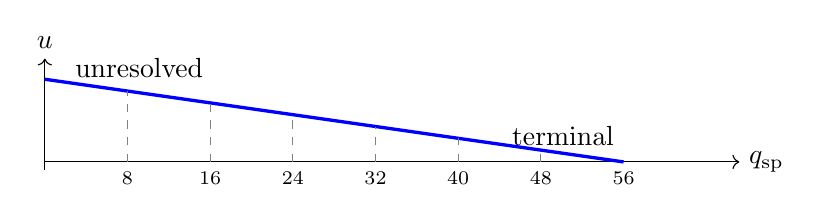
\begin{tikzpicture}[scale=1.05]
    \draw[->] (0,0) -- (8.4,0) node[right] {$q_{\rm sp}$};
    \draw[->] (0,-0.1) -- (0,1.25) node[above] {$u$};
    \draw[very thick, blue, domain=0:7, samples=120]
      plot (\x,{1-\x/7});
    \foreach \x in {1,2,3,4,5,6,7}{
      \draw[dashed, gray] (\x,0) -- (\x,{1-\x/7});
      \pgfmathtruncatemacro{\Klabel}{8*\x}
      \node[below] at (\x,0) {$\scriptstyle \Klabel$};
    }
    \node[above right] at (0.25,0.9) {unresolved};
    \node[above left] at (7,0.08) {terminal};
\end{tikzpicture}
\caption{Smooth protected visibility versus cumulative resolved rank depth.
The first six marks are finite scalar scale crossings; the seventh is the
asymptotic terminal endpoint.  They are not projector-rank events or, without
downstream predicates, named cosmological processes.}
\end{figure}

\subsection{C12 flat-gauge countermodel and exact geometric discharge target}
\label{p3e:app:c12-flat-gauge-countermodel}
This subsection records the negative and diagnostic details behind
Proposition~\ref{p3e:prop:c12-scheme-depth-closure-criterion}.  They protect
the positive response chain from treating an ordinary line-bundle
isomorphism as determinant ancestry.

On the scheme--depth base
\[
 B=I_+\times[0,7],\qquad
 \Phi(\sigma,q)=qL_\sigma,
\]
the determinant-dual and weight-$\lambda$ response sections and connections
are
\[
 \chi_1=e^{-\Phi},\qquad \nabla^{\rm sd}_1=d+d\Phi,
 \qquad
 \chi_\lambda=e^{-\lambda\Phi},\qquad
 \nabla^{\rm sd}_\lambda=d+\lambda d\Phi.
\]
Every connection is flat because $d^2\Phi=0$.  The positive gauge
\[
 g_\lambda=e^{(\lambda-1)\Phi}
\]
satisfies
\[
 d\log g_\lambda=(\lambda-1)d\Phi,
 \qquad
 \nabla^{\rm sd}_1(g_\lambda s)
 =g_\lambda\nabla^{\rm sd}_\lambda s,
 \qquad
 g_\lambda(\sigma,0)=1.
\]
Thus even a connection-preserving isomorphism normalized at the upper anchor
exists for every $\lambda>0$.  The mutation that replaces
$g_\lambda$ by the identity has residual
\[
 \nabla^{\rm sd}_1-\nabla^{\rm sd}_\lambda
 =(1-\lambda)d\Phi,
\]
which vanishes exactly at $\lambda=1$; this confirms that the calculation is
sensitive to the disputed weight.

The reason the nonconstant gauge is not the desired physical ancestry is its
dependence on an affine trivialization.  Under
$\sigma\mapsto\sigma+c$,
\[
 \frac{g_\lambda(\sigma+c,q)}{g_\lambda(\sigma,q)}
 =e^{(\lambda-1)qc}.
\]
For $\lambda\ne1$ this is a depth-dependent deformation and cannot be
absorbed into the single upper magnitude $U$.  A morphism induced by the same
fundamental associated determinant-dual representation has no such factor and
therefore has $\lambda=1$.

Independently, for every $\lambda>0$ set
\[
 \mathcal R_\lambda(q)=Ue^{-\lambda L_\sigma q},
 \qquad C_\lambda=Ue^{-7\lambda L_\sigma}.
\]
Then
\[
 0<C_\lambda<\mathcal R_\lambda(q)\le U,
 \qquad
 \frac{\log(\mathcal R_\lambda(q)/C_\lambda)}
      {\log(U/C_\lambda)}=1-\frac q7.
\]
Hence the normalized active coordinate and every descendant that factors
through it are identical throughout the counterfamily.  The family satisfies
the exact current MRESP hypotheses but changes
\(
 \lambda_{RD}=\log(U/C_\lambda)/(7L_\sigma)
\).
It is therefore a valid obstruction to deriving the weight from those
hypotheses.

A sufficient cross-role construction must generate a response transgression
directly from the fundamental determinant-dual associated line, before a
scheme origin or response trivialization is chosen, and then use its
normalized parallel section to transport the one dimensionful upper section.
The scalar-action compiler identifies the coefficient with its own density
dual. The stronger source-to-contact comparison is tested by
Theorem~\ref{p3b:thm:v2211-action-contact-certificate}. A successful
origin-certified $(\mathrm{ACD}_H)$ residual evaluation gives
$\mathcal R(q)=Ue^{-qL_\sigma}$ without a new fitted scalar. The printed
heat counterfamily proves that this success does not follow from the pairing
or common profile alone. Thus C12 is conditional on that actual evaluated
port; the neutral contact character and its roots remain unconditional within
their generated geometric owner.

\subsection{Scope witness and counterfamilies for the remaining common-owner relations}
\label{p3e:app:remaining-owner-counterfamilies}
The short positive results in the main text are premise-minimal only because
the following families preserve their current upstream hypotheses while
varying the disputed relation.

\subparagraph{Scope witness for the excluded off-diagonal extension.}
Fix \(g_x\) and the reciprocal diffeomorphism \(\beta\).  For \(c>0\), put
\[
                g_p^{(c)}:=c^{1/2}\beta_*g_x.
\]
In four dimensions a metric rescaling by \(a\) multiplies volume density by
\(a^2\), hence
\[
        \beta^*d\mu_{g_p^{(c)}}=c\,d\mu_{g_x}.
\]
Every member is smooth, nondegenerate, signature preserving, and isotropic;
the separately normalized compact Haar measures are unchanged.  Effective
density balance holds exactly at \(c=1\), proving that its Born-diagonal
derivation cannot be extended to independently parameterized effective
metrics.  Since no active theorem requests that extension, this family
delimits the theorem domain but does not define a residual premise.

\subparagraph{Response/EH section ratio.}
Fix \(\Lambda_{\rm EH}^2>0\), \(\alpha_\sigma>1\),
\(c_\sigma=\alpha_\sigma^{-7}\), and terminal data \((F_C,Z_C)=(0,1)\).
For each \(\kappa>0\), set
\[
 U_\kappa=\kappa\Lambda_{\rm EH}^2,
 \qquad C_\kappa=c_\sigma U_\kappa,
 \qquad
 u_\kappa(R)=\frac{\log(R/C_\kappa)}{\log(U_\kappa/C_\kappa)},
\]
and reconstruct
\[
 f_\kappa(R)
 =(R-C_\kappa)
 +\frac{16\sqrt{\alpha_\sigma}}{\Lambda_{\rm EH}^2}
  \int_{C_\kappa}^{R}(R-s)w_{\rm nl}(u_\kappa(s))u_\kappa(s)\,ds.
\]
Each dimensionless MRESP graph is admissible on the enlarged atlas in which
the response section is independently normalized; the terminal slope,
determinant-depth ratio, common action owner, covariance, convexity, and
terminal behavior obey the same post-response typed conditions, while
\[
 f_\kappa''(R)
 =w_{\rm nl}(u_\kappa(R))u_\kappa(R)
  \frac{16\sqrt{\alpha_\sigma}}{\Lambda_{\rm EH}^2},
 \qquad
 U_\kappa f_\kappa''(U_\kappa)
 =16\kappa\sqrt{\alpha_\sigma}.
\]
Every member therefore satisfies the algebraic PQTI relation, but
\(U_\kappa/\Lambda_{\rm EH}^2=\kappa\) is arbitrary.  For
\(\kappa\ne1\) the member fails the initial-object diagram of the
scalar-action coefficient compiler and therefore changes the frozen parent.
The family proves that common action membership and PQTI alone do not derive
\(\kappa_U=1\); it is not a countermodel to the stronger generated
identity-stage theorem.

\subparagraph{Normalized susceptibility amplitude.}
Fix \(U,C,\sigma,F_C,Z_C\) and the derived functions
\(w_{\rm nl}\) and \(u\).  For \(g>0\), define
\[
 f_g(R)=F_C+Z_C(R-C)
 +\frac gU\int_C^R(R-s)w_{\rm nl}(s)u(s)\,ds.
\]
Then
\[
 f_g(C)=F_C,
 \qquad f_g'(C)=Z_C,
 \qquad f_g''(R)=\frac gU w_{\rm nl}(R)u(R),
 \qquad Uf_g''(U)=g.
\]
All members share the metric, action owner, EH slope, tensorial Hessian
pullback, entropy coupling, convexity domain, and terminal Hessian decay.  A
positive same-action rescaling leaves \(g/Z_C\) invariant, so this parameter
is not an overall-normalization artefact.  It proves that the current grammar
without PQTI does not determine \(\widehat\gamma_\sigma\) or its horizontal
amplitude.  For generic \(g\) the family fails the normalized morphism
\(b_Q\) of Definition~\ref{p3e:def:primitive-quadratic-trace-inheritance};
it therefore proves the necessity of PQTI and is not a counterfamily within
the PQTI branch.

\subsection{Laurent endpoint counterchecks}
\label{p3e:app:laurent-endpoint-counterchecks}
For \(Q_\sigma>1\) and \(0<|\varepsilon|<1\),
\[
 D_\varepsilon(s)=Q_\sigma^{\,s+\varepsilon s(1-s)}
 \quad(0\leq s\leq1)
\]
is positive, continuous and strictly increasing, has endpoints
\(1,Q_\sigma\), and is not the multiplicative character unless
\(\varepsilon=0\).  Indeed its exponent derivative is
\(1+\varepsilon(1-2s)>0\), while its exponent is nonadditive.
This proves that endpoint data alone do not constitute a character.  It is not a countermodel to the later Paper~III-F coefficient-line representation, because for \(\varepsilon\ne0\) its logarithmic generator depends on \(s\) and it is not a one-parameter representation of the fixed generated automorphism \(A_Q\).

Treating \(-R_E+C_7\) as one complex density would require the very
same-owner identification absent between the two coefficient constructions,
so this counterroute still does not establish a cross-owner Einstein--Hilbert
normalization.  That limitation no longer leaves an independent terminal
zero-order datum: Paper~III-F derives the Euler-kernel-invariant terminal
intercept \(-C_7\) from the same Laurent--Legendre response, while the
intrinsic momentum curvature is known; its EH comparison and the
whole-action/source normalization remain actual evaluated ports.


\subsection{Born reciprocity and the affine action representative}
\label{p3e:app:born-affine-audit}
This subsection studies the bare unit-quadratic specialization only. It does
not change the protected dressing, the MRESP Hessian law, or the derived
Laurent--Legendre action branch. Set \(B=CU>0\), use \(R\) as the
scalar argument, and hold the independently typed linear coefficient fixed.
The remaining representatives are \(F_b(R)=R^2+b\).

\begin{proposition}[Centering is a section, not a physical vacuum selection]
\label{p3e:prop:born-centering-not-vacuum-selection}
The maps
\[
 s_-(F)=F-F(\sqrt B),\qquad
 s_+(F)=F-F(\sqrt B)+2B
\]
are both independent of constant shifts of \(F\). On every \(F_b\) they
return \(R^2-B\) and \(R^2+B\), respectively. Consequently the existing
reciprocal fixed point alone does not select the negative constant. Nor does
centering a component of the metric action determine the invariant
zero-order coefficient of the complete action.
\end{proposition}
\begin{proof}
A simultaneous constant in the two evaluations cancels in both maps.
Substitution proves their outputs. The selection of the zero value at the
fixed point is therefore an extra normalization condition, not a consequence
of the fixed point's existence. More generally a coefficient \(b\) in a
metric density is not an irrelevant numerical constant in the action:
\[
 \delta\!\int\!\sqrt{-g}\,b\,d^4x
 =-\frac b2\int\!\sqrt{-g}\,g_{\mu\nu}\delta g^{\mu\nu}\,d^4x.
\]
With \(Uf=UR+R^2+b\), the complete coefficient is
\[
 \overline{\mathcal F}=U(f-2\Lambda_{\rm ren})
 =UR+R^2+\beta,\qquad \beta=b-2U\Lambda_{\rm ren}.
\]
The same-action redistribution
\(b\mapsto b+\delta\),
\(\Lambda_{\rm ren}\mapsto\Lambda_{\rm ren}+\delta/(2U)\)
leaves \(\beta\) unchanged. Centering \(b\) without changing the full action
therefore cannot fix \(\beta\). This is the dimensionful form of
Paper~III-F, Theorem~\ref{p3f:thm:term-ren-zero-order-redundancy}.
\end{proof}

\subparagraph{The appropriate reconstruction retains the constant.}
Paper~I-D, Theorem~\ref{p1b:thm:born-euler-anticommutation} and
Proposition~\ref{p1b:prop:born-hessian-quotient-obstruction}, prove
\(\mathcal E\mathcal T_B=-\mathcal T_B\mathcal E\), while
\(\ker\mathcal E=\operatorname{span}\{R\}\). The full reciprocal pair is
therefore retained by Euler reconstruction but not by the Hessian quotient.
The physical comparison to test is
\(\mathcal E\overline{\mathcal F}=\mathscr Q_{C,U}\), not the Euler
remainder of an arbitrarily centered component. Paper~III-F,
Theorem~\ref{p3f:thm:born-coefficient-family-first-response} and
Theorem~\ref{p3f:thm:bare-born-potential-criterion}, now supply the stronger
bare same-action result: the generated coefficient-family connection detects
the constant affine mode, and the retained terminal value fixes the remaining
parallel Einstein section.  Hence terminal \(C^1\) is derived on that bare
branch rather than imposed.  This downstream constructor closure is not a new step inside PQTI.  In the
Paper~III-F also establishes the generated depth-two
coefficient character and its distinct inverse-Euler action
primitive. The exact structural
junction is derived as well; only occurrence of a particular physical history
remains separate under G0.


\begingroup
\small
\RaggedRight
\setlength{\emergencystretch}{3em}

\endgroup

\subsection{Native matrix tests inside the complete gravity-action comparison}
\label{p3e:sec:v226-gravity-comparison}
The coordinate-generated algebra and the degree-six chiral projectors of
Paper I-A may now be used without separately adjoining the round generators.
They provide an exact finite test for an actual native source or response
corner in the complete gravitational comparison.

\begin{corollary}[The native corner has a finite complete matching certificate]
\label{p3e:cor:v226-native-action-certificate}
After the actual two action words and their common native-corner maps are
specified, equality of that corner is equivalent to equality of its 137
dual coefficients. Every consumed metric/source jet is compared by the
same coefficient tests applied to the complete differentiated word.
\end{corollary}
\begin{proof}
Theorem~\ref{p1b:thm:v226-dual-coefficients} and
Corollary~\ref{p1b:cor:v226-source-jets} give necessity and sufficiency
on the supplied corner. A nonreducing corner map retains its actual
compression defects before the inverse is applied.
\end{proof}
This closes the availability of a complete finite test on that operator sort.
It does not assert equality of uncomputed coefficients, replace the physical
trace or metric measure, fix the normal band or boundary-datum norm, omit
tensor and source-orthogonal companions, or supply an absolute vacuum
allocation. The complete cap and Einstein/GHY matching keep their actual
operator, source, density and boundary ownership. No hierarchy or particle
normalization is recalibrated by the new operator basis.



\subsubsection{Conditional depth-two least-support comparison}
\label{p3e:subsec:complementary-laurent-action}

\begin{definition}[Positive-part Laurent data at depths two and seven]
\label{p3e:def:laur17-branch-data}
On an owner-typed ordered member
\(\mathrm{REG}_\sigma\in\mathfrak A_{\rm REG}^{+}\), put
\[
 A_\sigma:=\ln\alpha_\sigma>0,\qquad
 U:=\Lambda_{\rm EH}^2,\qquad
 C_j:=U\alpha_\sigma^{-j},\qquad j=2,7,
\]
and introduce
\[
 q(\scal):=-\frac{\ln(\scal/U)}{A_\sigma},
 \qquad K(\scal)=8q(\scal).
\]
Paper~III-D fixes the realized Laurent family.  Its mathematical identity
is Paper~I-D, Theorem~\ref{p1b:thm:laurent-family}~\cite{Kugelmann2026Paper1D},
with \(A=A_\sigma\), \(R=\scal\) and \(C=C_j\); for \(q>0\),
\begin{equation}
\label{p3e:eq:laur17-index-family}
 \boxed{
 n_j^{\rm L}(q)=
 \frac{\ln\!\cosh(jA_\sigma/2)
       -\ln\!\cosh[(j/2-q)A_\sigma]}
      {qA_\sigma},
 \qquad
 n_j^+:=\frac{n_j^{\rm L}+\sqrt{(n_j^{\rm L})^2}}2.}
\end{equation}
Thus \(n_j^+=\max(n_j^{\rm L},0)\): it agrees with the Laurent secant
where that secant is nonnegative and is exactly zero at and after \(q=j\).
It is not the mirrored continuation \(\lvert n_j^{\rm L}\rvert\).  On the
active side \(\scal\ge C_j\),
\begin{equation}
\label{p3e:eq:laur-active-response-family}
 \boxed{
 \mathcal H_j^{\rm act}(\scal)
 =\scal\left(\frac{\scal}{U}\right)^{n_j^+(\scal)}
 =\frac{\scal^2+UC_j}{U+C_j},
 \qquad
 \operatorname{ev}_{C_j}\mathcal H_j^{\rm act}=C_j.}
\end{equation}
The depth-two index dresses a coefficient only.  The rank-seven response is
the persistent nonlinear channel and alone owns the scalaron endpoint.
Consequently \(n_2^+=0\) removes the inflationary coefficient dressing but
does not terminate the nonlinear channel; \(n_7^+=0\) terminates that channel
at its attained value.  No function \(S(n)\), extra inflation monomial, or
second Einstein--Hilbert term is introduced.
On \((\mathrm{PQTI})\), define the full-support inflation amplitude
\begin{equation}
\label{p3e:eq:laur17-Q}
 \boxed{Q_\sigma:=8\sqrt{\alpha_\sigma}>1.}
\end{equation}
On the anchored octahedral member this is \(Q_0=8\sqrt\alpha\).
\end{definition}

\begin{definition}[Derived-later dressing, placement and exact interface]
\label{p3e:post:laur17-action-realization}
The active branch advertises three logically distinct outputs beyond the
Laurent family.  Their current status is
\[
\begin{array}{c|l}
 \mathrm{DCHAR}_{2}^{\rm coeff}&\text{derived positive coefficient character},\\
 \mathrm{ACT}_{2\mid7}^{\rm L}&\text{conditional on actual EXJET7 and action port},\\
 \mathrm{JUNC}_{2\mid7}^{\rm str}&\text{exact interface of the supplied response}.
\end{array}
\]
The later constructors are Paper~III-F,
Theorems~\ref{p3f:thm:v263-laurent-coefficient-character} and
\ref{p3f:thm:v263-dressed-born-legendre-descent}, together with the generic
GP exact-interface corollary of Paper~II-A.  They do not identify the
nonadditive physical secant coordinate with the additive character parameter.
The least-support theorem of Paper~III-D still selects \(j=2\) only on its
stated post-inflation turnover/disappearance role domain.  Whether an actual
solution history reaches or crosses the interface is G0 occurrence data; on
the source-free branch its local crossing germ is constrained by the
same-action field equation derived in Paper~III-F rather than by an inserted
microscopic profile.
\end{definition}

\begin{lemma}[Unique multiplicative dressing without an extra switch]
\label{p3e:lem:unique-character-dressing}
Let \(D:[0,1]\to\mathbb R_{>0}\) be continuous, satisfy
\[
 D(0)=1,\qquad D(1)=Q_\sigma,\qquad
 D(s+t)=D(s)D(t)
 \quad(0\le s,t, s+t\le1).
\]
Then
\begin{equation}
\label{p3e:eq:unique-character-dressing}
 \boxed{D(s)=Q_\sigma^{\,s}.}
\end{equation}
In particular, a replacement \(Q_\sigma^{S(s)}\) is compatible with the
same character law only when \(S(s)=s\).
\end{lemma}

\begin{proof}
The positive-character classification of Paper~I-C,
Proposition~\ref{p1b:prop:trace-coordinate}~\cite{Kugelmann2026Paper1C},
on \([0,1]\), with \(D(1)=Q_\sigma\), gives \(D(s)=Q_\sigma^s\).
Since \(Q_\sigma>1\), its exponential is injective, so any expression
\(Q_\sigma^{S(s)}\) satisfying the same character and endpoint conditions
has \(S(s)=s\).
\end{proof}

\subparagraph{Branch distinction.}
The depth-two Laurent factor is first retained here as a positive response
coefficient.  Paper~III-F later derives both its exponent-space character
and the unique same-action Legendre primitive.  The copied-response placement
is a separately conditional comparison,
not as the active physical action.

\begin{theorem}[Conditional depth-two dressed positive-response comparison]
\label{p3e:thm:raw-complementary-laurent-action}
On \((\mathrm{PQTI})\), define
\begin{equation}
\label{p3e:eq:laur17-dressing}
 \boxed{D_2(\scal):=Q_\sigma^{\,n_2^+(\scal)}.}
\end{equation}
The depth-two dressed rank-seven positive response is
\begin{equation}
\label{p3e:eq:raw-complementary-laurent-action}
 \boxed{
 \mathfrak P_{2\mid7}(\scal)
 :=D_2(\scal)\,\mathcal H_7^{\rm act}(\scal)
 =D_2(\scal)\frac{\scal^2+UC_7}{U+C_7},
 \qquad \scal\ge C_7.}
\end{equation}
Equivalently, on the positive-part strata,
\begin{equation}
\label{p3e:eq:raw-complementary-laurent-expanded}
 \mathfrak P_{2\mid7}(\scal)=
 \begin{cases}
 \dfrac{\scal^2+UC_7}{U+C_7},&C_7\le\scal\le C_2,\\[3mm]
 Q_\sigma^{n_2^{\rm L}(\scal)}
 \dfrac{\scal^2+UC_7}{U+C_7},&\scal>C_2.
 \end{cases}
\end{equation}
At the scalaron endpoint,
\begin{equation}
\label{p3e:eq:laur17-terminal-role-quotient}
 \boxed{\operatorname{ev}_{C_7}\mathfrak P_{2\mid7}=C_7.}
\end{equation}
Thus the endpoint is a zero-order attained response value, not a second
Einstein--Hilbert constituent.  In curvature-squared density normalization,
\begin{equation}
\label{p3e:eq:laur17-no-second-EH-density}
 \boxed{\mathcal I_{7,\rm nl}^{\rm term}=\Rp C_7
 =\Rp^2\alpha_\sigma^{-7}.}
\end{equation}
Paper~III-F subsequently proves that the unique terminal-normalized
\emph{physical} metric coefficient is obtained by integrating the locally
constituted fixed-depth susceptibility, not by inverse-Euler integrating
the raw Laurent secant:
\[
 \begin{aligned}
 \chi_{2\mid7}(R)&=D_2(R)\chi_7^{\rm jet}(R),\\
 f^{\rm L}_{2\mid7}(R)&=R-C_7+\int_{C_7}^R(R-x)\chi_{2\mid7}(x)\,dx,\\
 P_{2\mid7}(R)&:=Rf_R-f
 =C_7+\int_{C_7}^Rx\chi_{2\mid7}(x)\,dx.
 \end{aligned}
\]
The raw response \(\mathfrak P_{2\mid7}=D_2\mathcal H_7^{\rm act}\)
retains its Laurent readout role but is not equal to
\(P_{2\mid7}\) away from the certified endpoint.  This typing is
necessary because \(\mathfrak P'_{2\mid7}(C_7)=2C_7/(U+C_7)\),
while \(P_{2\mid7}'(C_7)=C_7\chi_{2\mid7}(C_7)=0\).
No independent \(\mathrm{ACT}_{2\mid7}\) selector remains on that retained
terminal-normalized branch.
\end{theorem}

\begin{proof}
Paper~III-D derives the positive-part Laurent exponent and its least-support
role statement.  Paper~III-F,
Theorem~\ref{p3f:thm:v263-laurent-coefficient-character}, constructs the
unique positive coefficient-line character and evaluates it on
\(n_2^+\), giving Eq.~\eqref{p3e:eq:laur17-dressing} without asserting
physical secant additivity.  The rank-seven active-response identity gives
Eq.~\eqref{p3e:eq:raw-complementary-laurent-action}; \(n_2^+=0\) at and below
\(C_2\) gives the displayed strata.  At \(C_7<C_2\), \(D_2=1\) and
\(\operatorname{ev}_{C_7}\mathcal H_7^{\rm act}=C_7\), proving the endpoint
and density statements.  The same-action action primitive is
Theorem~\ref{p3f:thm:v263-dressed-born-legendre-descent}.
\end{proof}

\begin{corollary}[Depth-two coefficient freeze and reflected label]
\label{p3e:cor:rank-one-exit-quadratic-grade}
On the active branch,
\begin{equation}
\label{p3e:eq:rank-one-exit-depth-two-scale}
 \boxed{C_2=U\alpha_\sigma^{-2},\qquad K(C_2)=16,
 \qquad n_2^+(C_2)=0,\qquad D_2(C_2)=1.}
\end{equation}
The same hierarchy value obeys the corroborating identity
\begin{equation}
\label{p3e:eq:depth-two-corroborating-identity}
 \frac{C_1^2}{U}=C_2.
\end{equation}
This equality does not select the dressing depth: tensor weight and hierarchy
depth are distinct typed coordinates unless an additional grade--depth bridge
is supplied.  At the actual coefficient freeze, the nonlinear response is
\begin{align}
\label{p3e:eq:rank-one-exit-exact-response}
 \mathfrak P_{2\mid7}(C_2)
 &=\mathcal H_7^{\rm act}(C_2)\nonumber\\
 &=\frac{C_2^2+UC_7}{U+C_7}
 =\frac{C_4+C_7}{1+\alpha_\sigma^{-7}}
 =C_4\frac{1+\alpha_\sigma^{-3}}
              {1+\alpha_\sigma^{-7}}.
\end{align}
Under the protected-octet reflection of
Theorem~\ref{p3c:thm:protected-octet-trace-reflection}, this depth-two label
has the scalar complement \(J(2)=6\).  That statement is a trace/scale
covariance only: it neither identifies the exit with the distinct crossing
\(\tau_6\) nor constructs radiation transfer, a dark-matter particle, or any
other physical event owner.
\end{corollary}

\begin{proof}
Paper~I-D, Theorem~\ref{p1b:thm:laurent-family}~\cite{Kugelmann2026Paper1D},
at \(j=2\) gives \(n_2^+(C_2)=0\), hence \(D_2(C_2)=1\).  Substitution into
Eq.~\eqref{p3e:eq:raw-complementary-laurent-expanded} yields the first two
expressions in Eq.~\eqref{p3e:eq:rank-one-exit-exact-response}.  Using
\(C_2^2/U=C_4\), \(C_7/U=\alpha_\sigma^{-7}\), and
\(C_7/C_4=\alpha_\sigma^{-3}\) gives the final two.  Separately,
\(C_1^2/U=C_2\) is direct hierarchy algebra.  The reflection statement
is Theorem~\ref{p3c:thm:protected-octet-trace-reflection}; its scope clause
proves the event-owner limitations.
\end{proof}

\begin{theorem}[Unique transverse depth-two coefficient-freeze event]
\label{p3e:thm:depth-two-transverse-event}
Let \(A_\sigma=\ln\alpha_\sigma>0\) and define, for \(q>0\),
\begin{equation}
\label{p3e:eq:depth-two-event-functional}
 F_{16}(q):=n_2^{\rm L}(q)
 =\frac{\ln\cosh A_\sigma
       -\ln\cosh[(1-q)A_\sigma]}{qA_\sigma}.
\end{equation}
On the active protected branch its unique zero is
\begin{equation}
\label{p3e:eq:depth-two-event-unique-zero}
 \boxed{F_{16}(q)=0\quad\Longleftrightarrow\quad q=2,}
\end{equation}
and that zero is transverse:
\begin{equation}
\label{p3e:eq:depth-two-event-q-derivative}
 \boxed{F_{16}'(2)=-\frac12\tanh A_\sigma\ne0.}
\end{equation}
Along the generated clock \(q_{\rm sp}(\tau)=7(1-e^{-\tau})\),
\begin{equation}
\label{p3e:eq:depth-two-event-clock-crossing}
 \boxed{\tau_{16}=\ln\frac75,\qquad
 \left.\frac{d}{d\tau}F_{16}(q_{\rm sp}(\tau))\right|_{\tau_{16}}
 =-\frac52\tanh A_\sigma\ne0.}
\end{equation}
Thus the \(K=16\) coefficient-freeze placement has an intrinsic action
readout satisfying the typed transverse-event criterion.  This theorem does
not turn the coefficient freeze into radiation transfer in physical time.
\end{theorem}

\begin{proof}
Paper~I-D, Theorem~\ref{p1b:thm:laurent-family}, gives the unique zero
\(q=2\); the endpoint calculation in
Theorem~\ref{p1b:thm:dressed-convexity}~\cite{Kugelmann2026Paper1D}
gives \((n_2^{\rm L})'(2)=-\tfrac12\tanh A_\sigma\).
For the generated clock, the common-rate formula in
Proposition~\ref{p1b:prop:trace-coordinate} applies to the visibility
semigroup constructed in Paper~III-C.  Solving
\(7(1-e^{-\tau})=2\) gives \(\tau_{16}=\ln(7/5)\), and
\(q_{\rm sp}'(\tau_{16})=5\).  The chain rule therefore gives
\(-\tfrac52\tanh A_\sigma\ne0\) on that clock.
\end{proof}

\begin{theorem}[Fixed-depth active susceptibility and convexity]
\label{p3e:prop:laur17-active-hessian}
Import Paper~III-D's fixed-depth rank-seven jet
$\chi_7^{\rm jet}(R)$ and Paper~III-F's generated depth-two coefficient
character $D_2(R)=Q_\sigma^{n_2^+(R)}$.  Because local configuration
variation does not differentiate the independent scheme/depth coefficient,
the physical local susceptibility on the diagonal background family is
\begin{equation}
\label{p3e:eq:laur17-active-hessian}
 \boxed{\chi_{2\mid7}^{\rm loc}(R)
 :=D_2(R)\chi_7^{\rm jet}(R)>0\qquad(R>C_7).}
\end{equation}
On the lower branch $C_7<R\le C_2$, $D_2=1$, so
\begin{equation}
\label{p3e:eq:global-positive-hessian-bound}
 \boxed{\chi_{2\mid7}^{\rm loc}(R)=\chi_7^{\rm jet}(R),
 \qquad 0<\chi_{2\mid7}^{\rm loc}(R)\le\frac2{U+C_7}.}
\end{equation}
The susceptibility extends continuously to zero at $C_7$.  Thus convexity is
generated while the scalaron susceptibility tends continuously to zero in the infrared;
no independent $\mathrm{CVX}_{17}$ or smoothing profile is introduced.
\end{theorem}

\begin{proof}
Paper~III-D constructs the local rank-seven jet after the hierarchy/depth
readout has been evaluated.  The depth-two object $D_2$ is independently a
coefficient character on the same frozen background member.  Local metric
variation therefore varies the configuration coordinate while holding that
coefficient fixed, so the second jet of the dressed nonlinear excess is the
scalar multiple $D_2\chi_7^{\rm jet}$.  Differentiating $D_2$ in this
operation would instead take a scheme/depth tangent and would change the
claim-complete variation space.  Positivity follows from $D_2>0$ and
Paper~III-D's positive local jet.  The lower-branch and terminal statements
use $D_2=1$ for $R\le C_2$ and
$\chi_7^{\rm jet}(C_7)=0$.
\end{proof}

\begin{proposition}[Depth-two K16 third-jet comparison]
\label{p3e:prop:v263-legendre-junction-measure}
The local susceptibility $\chi_{2\mid7}^{\rm loc}=D_2\chi_7^{\rm jet}$ is
continuous through $C_2$ because $D_2(C_2)=1$ on both sides.  Its one-sided
first background derivative has the finite step
\begin{equation}
\label{p3e:eq:v263-k16-hessian-step}
 \boxed{
 [\partial_R\chi_{2\mid7}^{\rm loc}]_{C_2}
 =D_2'(C_2^+)\chi_7^{\rm jet}(C_2)>0,}
\end{equation}
with the convention upper minus lower.  Hence the reconstructed metric action
is $C^2$ through K16 and has a finite third-jet kink there; it carries no
Delta-function atom in $dF$ or in the Hessian.  At $C_7$ the same susceptibility
vanishes continuously and the terminal Einstein one- and two-jets match.
\end{proposition}

\begin{corollary}[Smooth K16 and K48 local Hessians]
\label{p3e:cor:unique-k16-interior-action-junction}
Within $(C_7,U]$ there is no finite jump of the physical local Hessian at
K16.  The coefficient freeze appears one derivative later.  At K48,
\begin{equation}
\label{p3e:eq:k48-smooth-action-hessian}
 \boxed{
 f_{RR}(C_6)=\chi_7^{\rm jet}(C_6)
 =\frac{(1+n_7(C_6))(C_6^2-C_7^2)}{(U+C_7)C_6^2}>0,}
\end{equation}
and the action remains smooth there.  No independent microscopic width is
licensed at either event.
\end{corollary}


\section{Local Schur, source, boundary and matrix computations}
\label{p3g:sec:sources}
\subsection{Native polynomial continuation and clock comparison}
\label{p3f:app:v2190-native-continuation}

\subsubsection{A conditional complete scalar-source polynomial branch}
This is an optional domain extension of the local theorem, not a claim
that a local heat real-form germ has automatically acquired a global
physical continuation.  Adopt it only where the actual finite polynomial
action word is already licensed on its full coefficient space.

\begin{proposition}[Coercive native scalar and finite-source continuation]
\label{p3f:prop:v2190-polynomial-continuation}
Let a closed autonomous native scalar restriction have constant
\(M\succ0\), inherited kinetic form
\(L_{\rm cl}=\tfrac12v^TMv+(Cz+a_0)^Tv-U(z)\), and an injective real coefficient embedding
\(\Phi(z)=\sum_i z_iF_i\) into Hermitian fields, and retained polynomial
potential with leading term
\[
 U_4(z)=\frac1{16\pi^2}\int\operatorname{Tr}_F(\Phi(z)^4)\,d\mu.
\]
The integration measure is positive with finite volume, and the coefficient
Gram \(N_{ij}=\int\operatorname{Tr}_F(F_iF_j)d\mu\) is positive definite.
Include every remaining inherited potential term, with growth at most
quadratic, and the complete coordinate-only finite source \(H(z)\), whose
operator norm grows at most quadratically and whose coefficients are
\(C^3\) on the entire coefficient space.  Assume this entire word has the
actual full smooth polynomial coefficient chart \(\mathbb R^n\times\mathbb R^n\times
\mathcal O_{\sigma_0}\), with its constraints already discharged.
Then the joint characteristic field is complete for all real clock times.
\end{proposition}
\begin{proof}
If the fibre rank is \(r\) and the volume is \(V\), the pointwise eigenvalue
inequality and integral Cauchy--Schwarz give
\[
 \int\operatorname{Tr}\Phi^4\,d\mu
 \ge\frac1{rV}\left(\int\operatorname{Tr}\Phi^2\,d\mu\right)^2
 \ge\frac{\lambda_{\min}(N)^2}{rV}|z|^4.
\]
For a density matrix, \(|\operatorname{Tr}(\sigma H)|\le\|H\|\).
The complete action energy thus bounds the phase variables through
\(\mathcal E\ge a|P-Cz-a_0|^2+b|z|^4-c|z|^2-d\), with positive \(a,b\)
after absorbing any inherited lower-order potential terms.  Boundedness
of \(z\) and the shifted momentum gives boundedness of \(P\).
The state orbit is compact.
Conservation confines each trajectory to a compact sublevel set of the
smooth full polynomial chart.  The local continuation theorem then extends
the solution for every real time.  This proves neither a chosen vacuum nor
global gravity, nonlocal spectral action or continuum regularity.
\end{proof}

\subsubsection{Exact finite operation comparison}
On the regular joint chart of
Theorem~\ref{p3f:thm:v2190-joint-characteristic-flow}, an actual clock
operation with a licensed map to that chart equals the action-generated
one exactly when
\[
 X_{\rm op}q-v=0,\qquad
 X_{\rm op}P_i-L_{{\rm cl},q_i}
                   +\operatorname{Tr}(\sigma H_{,q_i})=0,\qquad
 X_{\rm op}\sigma+\frac{i}{\hbar}[H,\sigma]=0.
\]
These are finite coordinate versions of
\(\iota_{X_{\rm op}}(-d\alpha_{\rm tot})=0\); they introduce no threshold
or fitted coefficient.  The complete source-state tangent is tested on
its retained unitary orbit.  If the source action/quantization word already
declares this evolution target, the equalities are its constructed output,
not extra occurrence premises.  A Hopf-to-succession provenance composite
on a different vector-parent role cannot be compared without a licensed
cross-role map.  This diagnostic identifies that precise remaining arrow
without changing fixed terminal mass coefficients or choosing a vacuum.



\subsection{The separately declared native squared readout}
\label{p3f:app:native-source-square-readout}

This subsection adds the declared comparison operator
\(H_{u,\eta}=D_{u+\eta}^{\,2}\) to the native signed Dirac branch.
The squared readout is supplementary and is not used by the main signed
root or response theorems. Its conclusion is a quadratic energy root,
a quantified gap and two small offsets for an admitted positive target.
For the background notation retain
\(U=\lVert u\rVert_\infty\le1\),
\(\gamma_u=\sqrt3-3U/2\), \(g_u=\gamma_u/R\),
\(\delta_u=\gamma_u/9\), and the real inversion-odd profile and domain
of Theorem~\ref{p1b:thm:native-source-root-interval}.
If an application further requires \(\lVert u+\eta\rVert_\infty\le1\),
intersect this subsection's offset range with \(U+|\eta|\le1\).

\begin{corollary}[The declared square has a quadratic energy root]
\label{p3f:cor:native-source-square-root}
On the explicitly declared comparison branch \(H_{u,\eta}=D_{u+\eta}^2\),
and for \(|\eta|\le\delta_u=\gamma_u/9\), the ground is simple with
\[
 E_u(\eta)=\lambda_u(\eta)^2,\qquad
 \frac{\eta^2}{25R^2}\le E_u(\eta)
      \le\frac{9\eta^2}{4R^2},\qquad
 E'_u(0)=0,\qquad
 E''_u(0)=2\kappa_u^2\ge\frac{18}{25R^2}.
\]
Its gap to the rest of the squared spectrum is at least
\(2g_u^2/3\). For every supplied \(0<E<\gamma_u^2/(2025R^2)\)
there are exactly two offsets inside this interval, satisfying
\(\lambda_u(\eta)=\pm\sqrt E\).
\end{corollary}
\begin{proof}
The unique low eigenvalue has \(|\lambda|\le v\), whereas all the
other Dirac eigenvalues have absolute value at least \(g_u-v\), with
\(v\le g_u/6\). Thus its square is the unique ground and the gap
is at least \((g_u-v)^2-v^2\ge2g_u^2/3\).
The remaining claims follow from the native root interval and its
oddness. In particular a simple signed Dirac zero becomes a double
zero of this squared energy readout.
\end{proof}

The operator \(H_{u,\eta}\) in this corollary is declared in its premise.
The theorem does not identify it with the complete physical Hamiltonian,
and \(R\) remains the spatial round-metric radius. No root has been
calibrated against an electron terminal or a hierarchy scale.

For the dipole with \(|a|=1\), the exact Bessel normalization in
Proposition~\ref{p3f:prop:native-source-dipole-normalization} has the
dimensionless slope \(R\kappa_a=-1.200178363648686\ldots\).
This decimal is a supplementary numerical readout of the exact formula.

\begin{corollary}[Eighth-order energy of the declared quartic signed branch]
\label{p3f:cor:native-source-quartic-square}
Retain all hypotheses and \(\mathcal E_6(t)\) of
Theorem~\ref{p3f:thm:native-first-quartic-response}, and separately
declare the squared operator \(H(t)=(D_u+tV)^2\). If \(L_4\ne0\), its
local squared readout has
\[
 E(t)=\lambda(0,t)^2=L_4^2t^8+O(t^{10}),\qquad
 |E(t)-L_4^2t^8|\le2|L_4||t|^4|\mathcal E_6(t)|+|\mathcal E_6(t)|^2.
\]
When \(|t|\lVert V\rVert<g/2\), this is the simple ground of the full
squared operator, since all other signed eigenvalues have absolute
value at least \(g-|t|\lVert V\rVert\) and the continuing branch has
absolute value at most \(|t|\lVert V\rVert\).
\end{corollary}
\begin{proof}
Square the signed expansion and apply the triangle inequality to its two
error terms. The gap and low-branch bounds separate that square from
the rest of the squared spectrum on the stated range.
\end{proof}



\subsection{An exact native mixed fourth-order comparison}
\label{p3f:app:native-mixed-quartic-comparison}

This subsection supplies a declared bounded finite-rank insertion for the
native spatial operator. It tests the mixed fourth-order possibility and
its source visibility. The insertion is nonlocal; it is additional
comparison data, not a generated electron, gauge or complete-action term.
The construction acts on the full \(L^2\) operator with domain \(H^1\).
Its five-dimensional block is exactly reducing, rather than a truncation.

\subparagraph{Exact native reducing block.}
Write \(q=(q_0,q_1,q_2,q_3)\in S^3\), so inversion fixes \(q_0\)
and negates \(q_1,q_2,q_3\). The normalized real scalar harmonics
\[
 h_1=2q_1/\sqrt{V_R},\qquad h_2=\sqrt{24}\,q_0q_1/\sqrt{V_R},
 \qquad g_1=\sqrt3/R,\quad g_2=\sqrt8/R
\]
have \(\Delta_0h_j=g_j^2h_j\) and are inversion odd. The normalization
uses the sphere moments \(\langle q_1^2\rangle=1/4\) and
\(\langle q_0^2q_1^2\rangle=1/24\). They are orthogonal, as are their
normalized exact forms. Put
\[
 p_j=(0,dh_j/g_j),\quad m_j=(h_j,0),\qquad
 \mathcal H_5=\operatorname{span}\{s_0,p_1,m_1,p_2,m_2\}.
\]
On this orthonormal basis, \(B_Rp_j=g_jm_j\), \(B_Rm_j=g_jp_j\).
The Born signs are \((+,+,-,+,-)\); all five vectors are real.
Both \(B_R\) and the constant-offset \(J\) reduce \(\mathcal H_5\)
and its orthogonal complement.

For real dimensional constants \(a,c,d\), define on \(\mathcal H_5\)
\[
 V=i\begin{pmatrix}
 0&a&0&0&0\\-a&0&0&0&0\\0&0&0&d&c\\
 0&0&-d&0&0\\0&0&-c&0&0
 \end{pmatrix},\qquad V=0\quad\hbox{on }\mathcal H_5^\perp.
\]
It is bounded and self-adjoint, with
\(w=\max(|a|,\sqrt{c^2+d^2})\), and is reality odd. Its Born-even
part consists of the \(a,c\) links, while its Born-odd part is the
\(d\) link. The former is odd under the product antiunitary
\(\mathcal U\mathcal C\), and the latter under \(\mathcal U\).
Each separately protects a zero. For small amplitudes this also follows
from the explicit determinant below; no index value beyond the prior
protections is needed for this comparison.

\subparagraph{Calculated fourth-order shift.}
On the block at zero offset,
\[
 H_5(t)=\begin{pmatrix}
 0&iat&0&0&0\\-iat&0&g_1&0&0\\
 0&g_1&0&idt&ict\\0&0&-idt&0&g_2\\0&0&-ict&g_2&0
 \end{pmatrix}.
\]
The reduced midpoint inverse exchanges \(p_j,m_j\) with coefficient
\(1/g_j\). Directly,
\[
 \langle s_0,Vs_0\rangle=0,\qquad
 \langle s_0,VG_0Vs_0\rangle=0,\qquad
 L_4=-\frac{2a^2cd}{g_1^2g_2}.
\]
The two inner complementary links give the two equal contributions in
the last expression. Reality oddness kills all odd coefficients.
Thus \(acd\ne0\) gives an actual first fourth-order signed shift.
There is also an independent determinant calculation. Set
\[
 T_3(z)=z^3-z\{g_2^2+(c^2+d^2)t^2\}-2cdg_2t^2.
\]
Elimination of the two leaf vertices gives
\begin{equation}
 p_5(z)=\det(z-H_5)=(z^2-a^2t^2)T_3(z)
                      -zg_1^2(z^2-g_2^2).
 \label{p3f:eq:native-mixed-quartic-characteristic}
\end{equation}
Its constant term is \(2a^2cdg_2t^4\), while its unperturbed derivative
at zero is \(g_1^2g_2^2\), proving the same fourth coefficient.
The orthogonal spatial complement is unchanged at \(\eta=0\). For
\(|t|w<g_1/2\), the full spatial operator has precisely this one
eigenvalue near zero. Hence this coefficient belongs to the full operator.

For the explicit choice \(a=c=1/R\), \(d=2/R\),
\begin{equation}
 w=\sqrt5/R,\qquad
 \lambda(0,t)=-\frac{\sqrt2}{3R}t^4+O(t^6),\qquad
 \eta_*(t;0)=-\frac{2\sqrt2}{9}t^4+O(t^6).
 \label{p3f:eq:native-mixed-explicit-fourth}
\end{equation}
Here \(\kappa=-3/(2R)\). The signed remainder is certified by Theorem~\ref{p3f:thm:native-first-quartic-response} with \(r=\sqrt3/(4\sqrt5)\).
The squared operator has unique low ground for \(|t|w<g_1/2\), with
\(E(t)=2t^8/(9R^2)+O(t^{10})\).

\subparagraph{Exact offset equation and a controlled root error.}
Put \(\alpha=-3\eta/(2R)\), \(\beta=\eta/(2R)\),
\(z_\alpha=z-\alpha\), \(z_\beta=z-\beta\). The full offset block has
\[
 T_3=z_\alpha^2z_\beta-(g_2^2+d^2t^2)z_\alpha
                   -c^2t^2z_\beta-2cdg_2t^2,
\]
\[
 N_4=z_\beta T_3-g_1^2(z_\alpha z_\beta-g_2^2),\qquad
 p_5=z_\alpha N_4-a^2t^2T_3.
\]
For the explicit choice, let \(\widetilde p_5=R^5p_5(0)\) and
\(\widetilde N_4=R^4N_4(0)\). Direct expansion gives
\[
 \widetilde p_5=
 36\eta+12\eta t^2+\tfrac{11}{2}\eta t^4
 +\tfrac{99}{8}\eta^3+\tfrac{21}{4}\eta^3t^2
 +6\sqrt2\eta^2t^2+\tfrac{27}{32}\eta^5+8\sqrt2t^4,
\]
\[
 \widetilde N_4=24+\tfrac{33}{4}\eta^2+\tfrac{11}{4}\eta^2t^2
                     +4\sqrt2\eta t^2+\tfrac9{16}\eta^4.
\]
For \(\eta_{\dagger}=-(2\sqrt2/9)t^4\) and
\(|t|<t_0=\sqrt3/(90\sqrt5)\), Theorem~\ref{p3f:thm:native-shifted-signed-root}
applies to the full operator. Its scalar Schur residual is exactly
\(-p_5(0)/N_4(0)\), so
\begin{equation}
 |\eta_*-\eta_{\dagger}|\le
 5\left|\frac{\widetilde p_5(\eta_{\dagger},t)}
                  {\widetilde N_4(\eta_{\dagger},t)}\right|
 \le |t|^6.
 \label{p3f:eq:native-mixed-root-sixth-bound}
\end{equation}
For completeness, write \(k=2\sqrt2/9<1/3\). After the fourth-order
cancellation the absolute numerator is at most
\[
 |t|^6\{12k+\tfrac{11}{2}k|t|^2+6\sqrt2k^2|t|^4
 +\tfrac{99}{8}k^3|t|^6+\tfrac{21}{4}k^3|t|^8
 +\tfrac{27}{32}k^5|t|^{14}\}.
\]
Already for \(|t|\le1/2\), the braces are less than \(91/20\), and
the denominator is at least \(24-(16/9)|t|^6>23\).
Therefore the factor is less than \(5(91/20)/23<1\), proving the bound.
The next offset coefficient, obtained from the same exact equation, is
\(2\sqrt2/27\) at degree six. No numerical fit is used to assign it.

\subparagraph{Complete vector-source support.}
For source \(s_0\) at \(\eta=0\), the source resolvent is exactly
\begin{equation}
 \langle s_0,(z-H_5)^{-1}s_0\rangle=N_4(z)/p_5(z),\qquad
 N_4=zT_3-g_1^2(z^2-g_2^2).
 \label{p3f:eq:native-mixed-cyclic-resolvent}
\end{equation}
The determinant of its five-vector Krylov matrix is
\[
 \det[s_0,H_5s_0,H_5^2s_0,H_5^3s_0,H_5^4s_0]
 =-a^4g_1^3g_2(d^2-c^2)t^6.
\]
Thus \(a\ne0\), \(d^2\ne c^2\), \(t\ne0\) make the entire
\(\mathcal H_5\) cyclic: \(p_5\) is the minimal vector-source
polynomial and every one of its five distinct real roots has positive
residue \(N_4(z_j)/p_5'(z_j)\). The full orthogonal complement has
zero source weight, by exact reduction. At \(t=0\) the minimal
polynomial is \(z\), not the unreduced quintic. With offset the Krylov
factor \(g_2(d^2-c^2)\) becomes
\(g_2(d^2-c^2)+(\alpha-\beta)cd\), retaining visibility at the small
shifted root in the explicit example. Its zero residue tends to one;
more precisely it is \(1-t^2/3+O(t^4)\).

At zero offset write \(p_5=z^5-Az^3-Bz^2+Cz+D\), where
\[
 A=g_1^2+g_2^2+(a^2+c^2+d^2)t^2,\quad B=2cdg_2t^2,
\]
\[
 C=g_1^2g_2^2+a^2g_2^2t^2+a^2(c^2+d^2)t^4,
 \qquad D=2a^2cdg_2t^4.
\]
For the separately declared square, its complete source polynomial is
\begin{equation}
 p_{s_0,H_5^2}(E)=E(E^2-AE+C)^2-(D-BE)^2.
 \label{p3f:eq:native-mixed-square-polynomial}
\end{equation}
For the explicit example and nonzero sufficiently small \(t\), no
two signed roots have the same square. Indeed a pair \(z,-z\) would
require \(E=a^2t^2\) and
\(E^2-AE+C=g_1^2(g_2^2-a^2t^2)=0\), which is impossible in that
range. Thus the polynomial has five distinct source-visible energies,
with the inherited positive residues. A zero of an arbitrary sector
determinant or a tagged electron commutator is a different object.




\subsection{Coordinate capacity and the complete quantization domain}
\label{p3f:app:v2174-native-capacity-domain}
This subsection records the scope of the native coordinate bound and spherical
Legendre calculation. It assumes only their admitted action charts. It
derives no phase-space ceiling or actual electron quantum representation.

\subsubsection{What the scalar chart actually bounds}
Corollary~\ref{p3f:cor:v2174-scalar-coordinate-bound} bounds
$\operatorname{Tr}_F\Phi^2$ on $\mathscr F>0$.
Corollary~\ref{p8:cor:v2174-native-turning-momentum} instead retains the
mixed momentum $p_r^{\rm phys}/(\hbar V_3)=\alpha_\Phi w-C_0/w$ on
the supplied conditional turning member. Both are exact descendants of the
native action. A coordinate bound is not a bound on this conjugate momentum.
The lapse equation cannot be substituted into the Lagrangian before taking
the Legendre derivative: it eliminates a constraint variable only after
the independent velocity derivative has supplied the momentum. Replacing
that derivative by $2\alpha_\Phi w$ drops the scalar--metric term.

The expression does not establish that every finite $w$, or arbitrarily
large $w$, belongs to one licensed Cauchy family. All homogeneous-source,
Gauss, gauge, constraint and regularity guards remain. Nor is this chart
the stationary positive-Hessian/Gibbs domain used by C01. A complete
phase-space bound would require a same-owner theorem controlling both
coordinates and momenta on that actual domain.

\subsubsection{Finite readout bounds consume their own complete owners}
VI-A's bounded faithful metric realization
(Theorem~\ref{p8:thm:bounded-faithful-metric-realization}) gives a
family-dependent finite supremum on its occurring whole region, not a
universal numerical level or its attaining member. Its fixed-source density
maximum (Corollary~\ref{p8:cor:fixed-source-density-maximum}) consumes the
actual finite density operator and proper volume before taking a finite
spectral maximum. Similarly a ground energy, stationary response or
energy-period relation consumes its actual action, clock and state/period
domain. None of these operations by itself constructs an upstream Bose
occupation carrier. No independent energy ceiling, regulator or calibration
is added by these comparisons.

\subsubsection{The complete-member C01 route and its constructor antecedent}
Theorem~\ref{p3f:thm:v1148-finite-metric-constructor} consumes an already
licensed finite action/quantization word: actual clock, field and dual-field
embeddings, ordering, constraint and occupation projectors, and vacuum
allocation. It transports every action term consumed by that constructor and selects no
missing physical member.  This is one sufficient complete-member route to
the stationary electron response, not a universal requirement that every
entry of the total quantum representation be uniquely selected before its
source readout can be determined. A finite Bose mode rank is explicitly insufficient. The auxiliary
geometric pair presentation and coefficient dictionary supply different
output sorts; they do not exhibit this joint quantum word.

On this complete-member electron route the unexhibited compiled member is denoted
$\Gamma_e$. Its first complete expression is
\[
 [H_{\Gamma_e},q_e]P_0(H_{\Gamma_e})
 =\tfrac\pi2(Y_1+iY_2-(1+i)Y_3)P_0+[H_R,q_e]P_0,
 \quad H_R=H_{\Gamma_e}-V_W,
\]
\[
 Y_j=\sum_\alpha a_{\nu,j}^\dagger(K_\alpha j_{\rm ext})
                                    \otimes X_{\alpha,-}.
\]
The current coefficient is evaluated in V-C. The actual external,
dual-field and complete remainder matrices on $\Gamma_e$ are still
unexhibited. This is a stop at the named consumer's antecedent, not a new
occurrence, ground-state, conservation, visibility or pole obligation, and
not a proof that every future native constructor fails.
Once that complete member is supplied, reuse the licensed full Gibbs support,
all nonzero conserved-degree ground summands and both adjacent source legs.
The complete terminating tagged polynomial precedes its real visible roots,
which precede comparison with the fixed upstream $\varepsilon_e$ and any
actually source-authorized physical rest dictionary. Every contributing action term,
occupation return, weak/remainder mixed placement, contact and boundary
remains.  The metric constructor also retains its central allocation and
consumed metric/source derivatives. No actual root or terminal equality is asserted
by the auxiliary or local chart calculations here.


\subparagraph{The source-cyclic determination alternative.}
The pole-readout minimum is the actual complete source-cyclic action and
licensed exact stationary support, or a proof that their polynomial is
common throughout the independently licensed family.  Paper~IV,
Theorem~\ref{p4:thm:v2186-common-source-cyclic-polynomial}, gives the exact
cyclic-intertwiner criterion; its exact no-re-entry lemma justifies the
restriction only after the complete source action has been established.
This alternative does not require equality or uniqueness of total
Hamiltonians, total carrier dimensions or total occupation members.  It
does require every interaction and boundary contribution that can affect
that cyclic action or the physical support.  In particular the combined
$Y_j$ and $[H_R,q_e]$ returns above have not been evaluated on the actual
quotient, and their family-independence has not been proved.  No actual
electron root or terminal-to-pole equality is obtained by changing the
route description.

For a fixed chart, $H+cI$ has the same $\operatorname{ad}_H$, full ground
projector and tagged polynomial.  Consequently the unique scalar central
value is not a separate pole-location input.  This does not remove central
metric/source derivatives from the finite metric response, nor the scalar
value from absolute-energy, action-value or partition-function claims.
Residues require their actual transported state pairing; common roots
alone do not supply common weights.  Keep the fixed upstream terminal
coefficients and only the particle/rest and physical limit dictionaries
actually consumed by the claim.






\subsection{Stationary-contact formula comparisons}
\label{p3f:v2171:app:stationarychecks}
The following finite exterior-algebra examples test the general stationary
identities; their coefficients are not selected native physical data.
For one even interior with body $cu^2/2+gu^3/3$ and displacement terms
$uJ+u^2K/2$, where $J$ and $K$ have fermion degree two, $c\ne0$, and
there is no direct sixth-degree term, substitution gives
\[
 S^\partial_6=\frac{J^2K}{2c^2}-\frac{gJ^3}{3c^3}.
\]
The reproduction packet solves the interior equation in an eight-generator
exterior algebra through its entire nilpotent degree and separately checks
a two-interior inverse, mixed quartic contacts and moving-body source jets.
These verify coefficient identities rather than the uncomputed native
K16 field embedding. The complete classical stationary operation is
distinct from quantum integration and from elimination of odd particle modes.





\subsection{Exact metric-weighted quartic entry and cubature comparison}
\label{p3f:app:v1148-metric-quartic-entry}
This subsection illustrates the main-text moment evaluator. It selects a
tensor entry, not a physical source state or new scalar interaction.
Use the inherited quartic direction $(\lambda_{\rm sc}/4)h^4$ and
\[
 f_2=\sqrt{6/V_\gamma}(y_0^2-y_1^2),\qquad
 Q_3=\sqrt{8/V_\gamma}(y_0^3-3y_0y_1^2).
\]
Both have unit norm in $d\sigma_\gamma$ and eigenvalues $8$ and $15$.
Expanding their polynomial products and applying
Corollary~\ref{p3f:cor:v1148-metric-haar-coefficients} gives
\begin{align*}
 \int f_2^4&=\frac{27}{10V_\gamma},&
 \int Q_3^2f_2^4&=\frac{27}{4V_\gamma^2},\\
 \int|DQ_3|^2f_2^4&=\frac{2187}{28V_\gamma^2},&
 \int|D^2Q_3|^2f_2^4&=\frac{23895}{28V_\gamma^2}.
\end{align*}
All integrals use $d\sigma_\gamma$. In the native background-volume mode
coordinate $h=a^{-3/2}zf_2$, with that reference coordinate fixed, the
quartic contribution to the metric Hessian in order $(A,B,\psi,E)$ is
\[
 Q_{ab}^{(4)}=\frac{f_a\lambda_{\rm sc}z^4}{4a^6V_\gamma^2}
 \begin{pmatrix}
 -27/4&0&-81/4&-405/4\\
 0&2187/28&0&0\\
 -81/4&0&81/4&405/4\\
 -405/4&0&405/4&-5265/28
 \end{pmatrix}.
\]
The first metric jets vanish by parity. Quantization and compression retain
the original ordering and occupation word; this is one component of its
full vertex tensor. Its round coefficient agrees with the native round
mode action after clock conversion.

For this degree-14 second-jet product, direct fixed $2I$ cubature gives
\[
 \frac{V_\gamma}{120}\sum_{y\in2I}Q_3(y)^2f_2(y)^4
 =\frac{891}{128V_\gamma^2},\qquad
 \int Q_3^2f_2^4=\frac{864}{128V_\gamma^2}.
\]
The relative discrepancy is $1/32$. The design remains exact through
degree 11 and for the degree-8 round quartic; the discrepancy concerns
its extension to a different weighted word. Exact Haar moments supply
the coefficients for the local integral action. This comparison does not
license changing the physical momentum carrier $m_p=1$ or choosing a
new reciprocal-position resolution $m_x$.




\subsection{Angular Gram and a deformed-metric contact check}
\label{p3f:app:tt-angular-contacts}
This subsection checks the source coefficients. Its homogeneous $L=2$
directions and test masses are evaluation data, not a new physical source
selection. In the conventions of
Corollary~\ref{p3f:cor:level-one-quadrupole-incidence}, set
$K_j=2\sum_i\sigma_i\otimes J_i^{(j)}$ and
$d_A^0=-\sum_{ij}S_{A,ij}\sigma_i\otimes J_j^{(j)}$.
The relevant projectors and eigenvalues are
\[
 P_A=(K_{1/2}+3I)/4\quad(+5/2),\qquad
 P_B=(2I-K_1)/6\quad(-5/2),\qquad
 P_C=(K_1+4I)/6\quad(+7/2).
\]
Their spectator multiplicities are respectively $2,3,3$.
Direct spin-matrix multiplication gives
\[
 \operatorname{Tr}(P_Ad_A^0P_Ad_B^0)=\delta_{AB},\quad
 P_Bd_A^0P_B=0,\quad
 \operatorname{Tr}(P_Bd_A^0P_Cd_B^0)=\tfrac23\delta_{AB}.
\]
For example, $S=\operatorname{diag}(-1,-1,2)$ gives the last trace $4$
and $\operatorname{Tr}S^2=6$; rotational equivariance determines the five
normalized directions. Including spectators, the two angular response
weights are equal to $G=2(\hbar/a)^2/V_\gamma$.

An independent nonlinear geometry check uses a left-invariant metric
$\sum_i a_i^2\theta_i^2$ on $S^3$, $a_i=\sqrt{1+\epsilon y_i}$,
$\sum_i y_i=0$. Its constant-spinor Dirac eigenvalue is
\[
 c(\epsilon)=\frac{a_1^2+a_2^2+a_3^2}{2a_1a_2a_3}
  =\tfrac32+\tfrac38\epsilon^2\sum_i y_i^2+O(\epsilon^3).
\]
In the $j=1/2$ spin singlet the eigenvalue is
$c(\epsilon)-\sum_i a_i^{-1}=-3/2+O(\epsilon^3)$.
For the balanced two-branch ordinary massive energy, taking its square
root gives the averaged second derivative
\[
 \frac{(3/2)^2}{4\sqrt{m^2+(3/2)^2}}\sum_i y_i^2.
\]
Restoring $\hbar/a$, volume and harmonic normalization gives precisely
the $3/4$ pressure contact of
Theorem~\ref{p3f:thm:tt-dirac-vertex-contact}. The invariant frame has
$\Gamma_{ij}^{k}=\varepsilon_{ijk}$, so a constant symmetric tensor has
zero divergence; these are actual TT deformations. The packaged exact
matrix and nonlinear metric scripts also test the first higher band,
whose full energy curvature includes its zero-frequency induced response.



\subsection{Spatial heat response and its Cartan curvature}
\label{p3f:app:m8td-heat}
This subsection evaluates the specified spatial trace and proves its
curvature sign. It is a diagnostic of the retained operator, rather than
the stability theorem for the complete coupled effective action. The
round realization and doublet multiplicity are those of
Theorem~\ref{p3f:thm:m8td-hodge-dirac}.

\begin{proposition}[Exact trace and negative Cartan curvature]
\label{p3f:prop:m8td-heat-curvature}
Put $h=t/R^2>0$, $b_n=n(n+2)$, $c_n=(n+1)^2$ and $\delta=f-1/2$.
The uninserted spatial doublet trace is
\begin{align}
 Z(h,\delta)&=\operatorname{Tr}e^{-t\mathcal D_f^2}
 =e^{-9h\delta^2}
 +2\sum_{n\ge1}c_ne^{-h(b_n+5\delta^2)}
       \cosh(2h\delta\sqrt{b_n+4\delta^2})\nonumber\\
 &\quad+2\sum_{n\ge1}b_ne^{-h(c_n+\delta^2)}
       \cosh(2h\delta\sqrt{c_n}).
 \label{p3f:eq:m8td-heat-trace}
\end{align}
It is even in $\delta$, and for every $h>0$,
\begin{equation}
 Z_\delta(h,0)=0,\qquad
 Z_{\delta\delta}(h,0)<
 \begin{cases}-2\sqrt{\pi h},&0<h\le1,\\
 -(462/47)h,&h\ge1.
 \end{cases}
 \label{p3f:eq:m8td-heat-curvature}
\end{equation}
\end{proposition}
\begin{proof}
The exact series is Paper~I-D,
Proposition~\ref{p1b:result:exact-heat-trace-and-parameter-evolution};
its differentiated-series sign and both quantitative bounds are
Proposition~\ref{p1b:prop:heat-curvature}
\cite{Kugelmann2026Paper1D}. The definitions of \(h\), \(\delta\),
\(b_n\) and \(c_n\) coincide, and both results concern this uninserted
spatial doublet trace.
\end{proof}

A nonzero positive linear combination of these traces inherits the
negative curvature when differentiation under that combination is
justified. The different functional $-\log Z$ has positive curvature at
the same stationary point. Thus an action must be identified before a
stability interpretation is made. Clocks, finite-carrier restrictions,
odd fields, matter, metric and boundary contributions are not erased by
this spatial computation.

For smooth zero-order perturbations obeying
Theorem~\ref{p3f:thm:m8td-protected-zero}, spectral pairing also gives
\[
 \operatorname{Tr}(\mathcal Ue^{-tD^2})=1\qquad(t>0).
\]
Each nonzero graded pair cancels and the graded zero multiplicity is the
index. This supplementary inserted readout does not replace the source's
uninserted action.

\subsection{Explicit protected mode, contractions and supplied histories}
\label{p3f:app:m8td-examples}
The main dipole calculation is the cohomogeneity-one representative of the
protected family and lies in the longitudinal subclass $\Omega_h=0$; its
absence of a coexact one-form component is therefore a symmetry reduction,
not a property of a generic reciprocal-odd Cartan background. The time
evolution below additionally assumes a supplied homogeneous Lorentzian
history. Neither calculation selects a physical state or history.

The smooth dipole zero and its removable zero-amplitude limit are now
stated in the main operator chain,
Proposition~\ref{p3f:prop:m8td-explicit-nonconstant-zero};
Proposition~\ref{p3f:prop:native-source-dipole-normalization}
evaluates its exact norm and constant-offset slope. The supplementary
contractions and supplied-history evolutions below do not select a
physical state or a history.

For the pointwise unit singlet,
$\langle\xi_0,\sigma_aI_b\xi_0\rangle=-\delta_{ab}/2$.
Writing a small gauge variation as $a_a=i b_a{}^bI_b$ gives
\[
 Pc(a)P=\frac1{2V_R}\int\sum_a b_a{}^a\,d\mu.
\]
The constant Cartan variation has $b_a{}^b=-2\delta\delta_a{}^b/R$,
giving $-3\delta/R$. Its complementary coupling vanishes, so the
crossing is exact rather than just first order. A Clifford-valued odd
term requires its own contraction, as stipulated in the main theorem.

On a constant-radius Lorentzian comparison branch, choose
$\eta=c_{\rm op}t/R$, $\hbar=1$ and the Weyl sign
$i\partial_\eta\psi=R\mathcal D_{f(\eta)}\psi$. Then
\[
 a_0(\eta)=a_0(\eta_0)\exp\left(3i\int_{\eta_0}^{\eta}\delta(s)\,ds\right).
\]
With this supplied time and Weyl convention, the parameter-evolution
block of Paper~I-D,
Proposition~\ref{p1b:result:exact-heat-trace-and-parameter-evolution}
\cite{Kugelmann2026Paper1D}, gives the scalar--exact pair's Hamiltonian
\[
 H_n=-\delta I+\sqrt{n(n+2)}\,\sigma_x-2\delta\sigma_z.
\]
A continuous diagonalizing angle has
\[
 \theta_n'=\frac{2\sqrt{n(n+2)}\delta'}{n(n+2)+4\delta^2},\qquad
 |\theta_n'/2|\le|\delta'|/\sqrt{n(n+2)}.
\]
The coexact modes acquire the phases of $\delta\pm(n+1)$. These equations
do not impose adiabaticity. Reversing the Weyl sign reverses the time
Hamiltonian. The homogeneous singlet crossing has a literature precedent
\cite{GibbonsSteif1993Sphalerons}; the formulas here follow from the
explicit retained operator and the full Hodge spectrum.

For an already supplied general isospin $\iota$, the midpoint scalar
Casimir minimum follows by $j+k=\iota$ and the smallest permitted
$|j-k|$: it is $\iota/R^2$ with multiplicity $(\iota+1)^2$ for integer
$\iota$, and $(\iota+1/4)/R^2$ with multiplicity
$2(\iota+1/2)(\iota+3/2)$ for half-odd-integer $\iota$.
This supplementary formula does not generate further physical representations.

\subsection{Hermitizing-line representation note}
\label{p3f:app:v177-hermitizing-line}
The uniqueness used in
Theorem~\ref{p3f:thm:v177-local-clocked-fermion-jet} is a statement about the
irreducible four-component complex spinor factor, not about the full
spinor--internal tensor product.  If $A_{\rm h}$ hermitizes the Clifford
matrices and $T$ commutes with every Clifford matrix, then
$A_{\rm h}T$ is another hermitizing candidate only when the corresponding
adjoint condition is satisfied.  On the irreducible spinor factor the
commutant is $\CC I$ and Hermiticity reduces this to the real line.  On an
additional internal multiplicity space the commutant becomes larger; choosing
one of those positive matrices would be an extra wavefunction insertion and
is therefore excluded on the named uninserted branch.  This is why the local
compiler removes a scalar kinetic ambiguity without claiming a general
family-dependent $Z_F$ theorem.

\subsection{Coarse homogeneous entropy diagnostic}
\label{p3f:app:coarse-entropy}
\begin{corollary}[Coarse macrocell entropy on a homogeneous branch]
\label{p3:prop:thermodynamic-arrow}
For a fixed comoving reciprocal-position region with
\(V_x=V_{x,0}a^3\) and fixed compact momentum volume \(V_p\), define
\[
S_{\rm cg}=S_0+\log\frac{V_x}{V_{x,\rm cell}}
              +\log\frac{V_p}{V_{p,\rm cell}}.
\]
Then
\[
\frac{dS_{\rm cg}}{d\tilde t}=3H,
\qquad H=\frac{\dot a}{a}.
\]
Thus, on the inherited scalar-succession orientation, increasing coarse
macrocell entropy is equivalent to a solution with \(H>0\).  It neither
chooses an additional time orientation nor proves that a solution is
expanding.
\end{corollary}

\begin{proof}
The momentum volume and both primitive cell volumes are constant, while
\(d\log V_x/d\tilde t=3\dot a/a\).
\end{proof}

\subsection{Smooth-profile tolerance diagnostic}
\label{p3f:app:smooth-profile-resolution}
A full-support action profile does not define an exact finite frontier.  For
example, suppose the scalar heat weight
\[
 w_k(\widetilde t)
 :=\exp\!\left(
 -\frac{k(k+2)}
 {(\Lambda_{\rm cut}a(\widetilde t))^2}\right)
\]
is separately declared operationally active exactly when
\(w_k\ge\varepsilon\), with \(0<\varepsilon<1\).  Then the corresponding
tolerance resolution is
\[
 \boxed{
 m_{x,\varepsilon}^{\rm inst}(\widetilde t)
 =\max\!\left\{1,
 \left\lfloor
 \sqrt{1+(\Lambda_{\rm cut}a(\widetilde t))^2
 \log(1/\varepsilon)}-1
 \right\rfloor\right\}.}
\]
Indeed, \(w_k\ge\varepsilon\) is equivalent to
\[
 k(k+2)\le
 (\Lambda_{\rm cut}a)^2\log(1/\varepsilon).
\]
The tolerance \(\varepsilon\) is operational resolution data; it is not
derived from \(a\), \(\Lambda_{\rm cut}\), or the common \(\Dcl\) action
profile.  Exactly, cumulative retention takes the supremum of the displayed
integer resolutions over the past interval.  If the scale supremum \(A_*\) is
attained, one may replace \(a\) by \(A_*\); if it is not attained at an exact
tolerance threshold, the same one-level floor correction as in
Theorem~\ref{p3:thm:exact-spectral-resolution-staircase} applies.

\subsection{Born-even fixed-set diagnostic}
\label{p3f:app:born-even-fixed-set}

\begin{definition}[Optional eight-dimensional Born diagnostic]
\label{p3f:def:born-eight-dimensional-diagnostic}
On \((\mathrm{BULK}_8)\), let
\[
 Y_8=(S_x^3\times S_p^3)\times(S_t^1\times S_E^1),
 \qquad
 \mathcal B(x,p,t,E)=(p,x,E,t),
\]
with the auxiliary metrics, normalized measures, and commuting nonnegative
Laplace-type operator \(L_8\) declared in
Definition~\ref{p3:def:lat-pol-csa-gred-hypotheses}.  Then
\[
 \operatorname{Fix}(\mathcal B)
 \cong S^3_{\rm diag}\times S^1_{\rm diag},
 \qquad \dim\operatorname{Fix}(\mathcal B)=4,
 \qquad P_+=\frac{1+\mathcal B}{2}.
\]
This is an eight-dimensional comparison object.  It is not the
seven-dimensional bundle \(X_7\), and its scalar-circle metrics have no
physical status in the main reduction.
\end{definition}

\begin{lemma}[Born-even bulk projection factor]
\label{p3:lem:born-even-bulk-projection-factor}
Under \((\mathrm{BULK}_8)\), the ordinary eight-dimensional bulk
heat-kernel coefficient of \(P_+e^{-tL_8}\) carries the factor
\[
 \boxed{\beta_{\rm B}^{\rm bulk}=\frac12}.
\]
The remaining equivariant contribution is supported on the four-dimensional
Born fixed set and belongs to lower-dimensional fixed-set coefficients.  No
seven-dimensional gauge coefficient follows without
\((\mathrm{MATCH}_{8\to7})\).
\end{lemma}

\begin{proof}
For completeness, the standard projected heat trace is
\[
 \Tr(P_+e^{-tL_8})
 =\frac12\Tr(e^{-tL_8})+\frac12\Tr(\mathcal B e^{-tL_8}).
\]
Under \((\mathrm{BULK}_8)\), the first term supplies one half of each ordinary
eight-dimensional bulk coefficient.  The second term is
localized on the Born fixed set.  The standard equivariant expansion near a
fixed component of dimension \(d_F\) begins at order \(t^{-d_F/2}\)
\cite{Wang2009EquivariantHeat}.  In the auxiliary branch used here the ordinary
eight-dimensional bulk begins at \(t^{-4}\), whereas the four-dimensional Born
fixed component begins at \(t^{-2}\).  It therefore contributes to
lower-dimensional fixed-set coefficients rather than the ordinary leading
eight-dimensional bulk coefficient.  This proves
\(\beta_{\rm B}^{\rm bulk}=1/2\) on the optional diagnostic.  It does not
identify that coefficient with the seven-dimensional reduction; such use
requires \((\mathrm{MATCH}_{8\to7})\).
\end{proof}

\begin{corollary}[Typed eight-to-seven coefficient routing]
\label{p3f:cor:typed-eight-to-seven-routing}
Assume \((\mathrm{BULK}_8)+(\mathrm{MATCH}_{8\to7})\).  If
\(\mathcal C_{8,{\rm bulk}}^{\rm raw}\) is the ordinary unprojected
eight-dimensional bulk coefficient, then the routed coefficient is
\[
 \widehat{\mathcal C}_{8,{\rm bulk}}^{(+)}
 =\widehat{\mathcal R}_{8\to7}
   \left(\frac12\mathcal C_{8,{\rm bulk}}^{\rm raw}\right)
 =\mathcal C_{\rm EH},
\]
where \(\widehat{\mathcal R}_{8\to7}\) is the declared normalized-volume
reduction map.  This equality is exactly the content of the matching bridge;
it is not derived from \((\mathrm{BULK}_8)\).  Once matched, the coefficient
may be used as the \(\mathcal C_{\rm EH}\) antecedent of the
seven-dimensional theorem, with the factor \(1/2\) applied exactly once.
\end{corollary}

\subsection{Left--right normalization diagnostic}
\label{p3f:app:lr-diagnostic}
Inside \((\mathrm{GRED}_7)\), inversion exchanges the two simple isometry ideals
of the same round vector fibre.  An independent relative coefficient would
therefore require changing the invariant metric/generator normalization or
adding a left--right distinguishing projector or weight.  Such a theory lies
outside the symmetric GRED branch.  A common rescaling instead changes
\(\kappa\) in \((\mathrm{CAL}_{\rm GRED}(\kappa))\) and leaves the geometric
equality intact.  This negative diagnostic is not needed in the positive proof
of the equality.

\subsection{Optional scalar-circle metric branch}
\label{p3f:app:scalar-circle-metric}
The constitutional scalar \(U(1)\) role is dimensionless.  If a later theory
adds an explicit scalar-circle metric calibration \((\mathrm{SCAL}_{\rm fib})\)
with radius \(\rho_{\rm fib}>0\), and if the same auxiliary bulk matching is
extended to a separately declared circle connection, then one may define conditionally
\[
 g_{\rm fib}^{-2}:=\rho_{\rm fib}^2\,\mathcal C_{\rm EH}.
\]
Here \(\mathcal C_{\rm EH}=f_2\Lambda_{\rm cut}^2/48\) is the same
protected Einstein coefficient used in the vector \((\mathrm{GRED}_7)\)
branch.  Neither
\(\rho_{\rm fib}\) nor this coupling is a theorem of the main III-F
constitution.

If this optional branch is strengthened further to a flat metric on the full
scalar torus together with a constant-curvature unitary connection on an
integer-degree power of the primitive Poincar\'e line, then
Proposition~\ref{p3a:prop:v212-scalar-line-spectrum-handoff} and Paper~I-C,
Theorem~\ref{p1b:thm:g13-landau},
Proposition~\ref{p1b:prop:g13-dirac}, and
Proposition~\ref{p1b:prop:relational-scalar-line-operators}
\cite{Kugelmann2026Paper1C}, fix the corresponding scalar Landau/Dirac
spectra and heat trace.  For nonzero degree the last proposition also fixes
the typing: this is a twisted line-bundle operator sector, not the untwisted
scalar-function algebra.  This is theorem composition on the enlarged
optional metric/connection branch; it does not supply the metric, connection,
physical kinetic normalization, or an extra family multiplicity on the native
III-F branch.

\subsection{Forward realization interface}
\label{p3f:app:forward-realization}
If a later paper supplies the occurring minimal local action and proves that a
concrete macroscopic branch satisfies
\((\mathrm{VDOM}_x^{\min})+(\mathrm{QLOC})\) and the local protected
spectral/EH hypotheses used here, then
Corollary~\ref{p3:cor:d3_derived} may be instantiated on that branch.  This is ordinary theorem composition.  The cotangent target and reciprocal generator-germ physical co-realization
are already derived; only the calibrated physical-polar domain when that polar
is used, the action occurrence, and the later locality hypotheses remain to
be supplied on the concrete branch.

\subsection{The unreduced Born-curvature test}
\label{p3f:app:born-comparison-curvature-test}
\begin{proposition}[Curvature and conjugate completion]
\label{paper3g:proposition:atlas-curvature-and-conjugate-completion-bbc8aec}

For the canonical Born connection
\(\omega_B=\tfrac12(\theta_x+\theta_p)\), on anti-diagonal tangent
vectors one has
\[
 \Omega_B((X,-X),(Y,-Y))=-[X,Y].
\]
Its curvature spans \(\mathfrak{su}(2)\); the defining left and
right fibre-spin extensions are nonflat.  The unreduced right
curvature has no nonzero fixed vector and no invariant line in
\(\operatorname{Sym}^2W_R^*\).
\end{proposition}
\begin{proof}
Insert the Maurer--Cartan equations in
\(d\omega_B+\tfrac12[\omega_B,\omega_B]\).
The connection term vanishes on the anti-diagonal arguments and
the two exterior derivatives give \(-[X,Y]\).
Commutators span \(\mathfrak{su}(2)\).  The symmetric square of
the defining doublet is the irreducible three-dimensional
representation, so it has neither an invariant vector nor a
one-dimensional invariant subrepresentation.  A parallel line or
tensor must satisfy the corresponding curvature invariance.
Passing to a block-diagonal conjugate completion preserves the
curvature on each block and leaves its absent cross block zero.
\end{proof}

The flat sign-holonomy connection on \(\mathcal O\) is not a
replacement for either Born anchor.  The physical comparison
problem must retain its own base, target action and connection
intertwiner rather than deleting one of these anchors.

\begin{corollary}[Trivial bundle, nontrivial holonomy]
\label{p3f:cor:v181-trivial-bundle-nontrivial-holonomy}
The global section identified in Paper~III-B is the trivialization of
Paper~I-C, Theorem~\ref{p1b:thm:relative}
\cite{Kugelmann2026Paper1C}, for the principal
$SU(2)_{\rm diag}$ bundle $X_7^{\rm cmp}\to K_{\rm rel}$.
Paper~I-C, Theorem~\ref{p1b:thm:homogeneous}, and its generated-background
specialization in Corollary~\ref{p3f:cor:v181-full-born-holonomy} give full
restricted holonomy for its canonical connection.  Thus bundle triviality
does not imply flatness.  Moreover, on the three-dimensional $SU(2)$ factor
the curvature has no nonzero four-form square, so this canonical anchor alone
carries no second-Chern density.  No conclusion is drawn for later generated
gauge bundles on four-dimensional physical bases.
\end{corollary}




\subsection{Exceptional symmetry after kinetic normalization}
\label{p3f:app:v179-exceptional-kinetic-symmetry}

This conditional symmetry test supplements the local response compiler.
It requires both group actions to preserve one complete quadratic owner
on one background, with all its marks retained.

\begin{proposition}[Symmetry of the normalized quadratic operator]
\label{p3f:prop:v179-normalized-symmetry}
Suppose \(Z>0\), \(K=K^\dagger\), and
\[
 D(g)^\dagger ZD(g)=Z,\qquad D(g)^\dagger KD(g)=K.
\]
Then \(\widehat D(g)=Z^{1/2}D(g)Z^{-1/2}\) is unitary and commutes with
\(\widehat M^2=Z^{-1/2}KZ^{-1/2}\).
If the embedded \(2O\) and \(2I\) are both such symmetries in one
continuous \(\mathrm{SU}(2)\) representation, then
\[
 \widehat M^2=\bigoplus_j I_{V_j}\otimes B_j
 \quad\hbox{on}\quad\bigoplus_j V_j\otimes M_j .
\]
The Hermitian multiplicity operators \(B_j\) remain action data.
\end{proposition}
\begin{proof}
Conjugating the two preserved forms by \(Z^{-1/2}\) gives unitarity and
invariance of \(\widehat M^2\), hence commutation.  By
Theorem~\ref{p1:thm:2O-2I-generate-SU2}, the two embedded groups generate
a dense subgroup of \(\mathrm{SU}(2)\).  Continuity extends commutation
to the whole group.  The irreducible decomposition gives the displayed
multiplicity form.
\end{proof}

A vacuum or retained mark can reduce the symmetry; covariance of its
family does not imply invariance of each member.  In particular, the
recentered coset-plane actions in
Appendix~\ref{p1:app:v179-exceptional-two-plane} are not thereby
restrictions of one common continuous representation.


\subsection{Affine Schur criterion and reciprocal rigidity}
\label{p3f:app:v199-affine-schur}
This is a sufficient comparison class for a conditional local-\(L\)/G26-GLOBAL comparison, with its additional hypotheses
displayed explicitly.  Take a scalar boundary and an exactly affine parent
\[
 H(y)=\begin{pmatrix}a_0+ya_1&(b_0+yb_1)^\dagger\\
 b_0+yb_1&C_0+yC_1\end{pmatrix},\qquad C_0>0,
\]
on an interval containing zero on which \(C_0+yC_1>0\).
Set \(z_0=-C_0^{-1}b_0\), \(r=b_1+C_1z_0\),
\(\lambda_0=a_0-b_0^\dagger C_0^{-1}b_0\), and
\(d_0=a_1+2\operatorname{Re}(b_1^\dagger z_0)+z_0^\dagger C_1z_0\).

\begin{proposition}[All-order affine Schur remainder]
\label{p3f:prop:v199-affine-schur-remainder}
The scalar Schur complement is exactly
\[
 \lambda(y)=\lambda_0+d_0y-y^2r^\dagger(C_0+yC_1)^{-1}r.
\]
If \(\lambda_0=0\) and \(d_0=1\), then
\[
 \lambda(y)=y\text{ on the interval}
 \quad\Longleftrightarrow\quad r=0
 \quad\Longleftrightarrow\quad \lambda''(0)=0.
\]
\end{proposition}
\begin{proof}
In Paper~I-D, Theorem~\ref{p1b:thm:all-order-schur}
\cite{Kugelmann2026Paper1D}, this affine family has residual
\(R_0(y)=yr\) and fixed-lift value \(\lambda_0+d_0y\), giving the
exact identity. Moreover \(\lambda''(0)=-2r^\dagger C_0^{-1}r\);
\(C_0>0\) gives the asserted equivalences.
\end{proof}

\begin{proposition}[Concavity and physical reciprocity force linearity]
\label{p3f:prop:v199-reciprocal-concavity}
Suppose \(\lambda\) is concave on \([0,\infty)\), positive on
\((0,\infty)\), \(\lambda(0)=0\), \(\lambda'_+(0)=1\), and the
same normalized physical response obeys
\(\lambda(y)\lambda(1/y)=1\).  Then \(\lambda(y)=y\).
\end{proposition}
\begin{proof}
Apply the scalar case of Paper~I-D,
Theorem~\ref{p1b:thm:matrix-rigidity} \cite{Kugelmann2026Paper1D},
on every finite reciprocal window to obtain \(\lambda(y)=y\).
The affine parent supplies the needed concavity because its Schur response
is the infimum, over the interior displacement, of affine functions of
\(y\). If both full affine coefficients are positive, it also supplies
positivity and monotonicity on the positive source axis.
\end{proof}


\begin{theorem}[Matrix reciprocity rigidity on a bounded source window]
\label{p3f:thm:v203-matrix-reciprocal-rigidity}
On a fixed finite boundary Hilbert space, let $\mathcal K(y)$ be Hermitian
and operator-concave on $[0,Y]$, $Y\ge1$, with
$\mathcal K(0)=0$, $\mathcal K'_+(0)=I$, and $\mathcal K(y)>0$ for $y>0$.
Suppose a retained unitary $B$ obeys
\[
 \mathcal K(1/y)=B\mathcal K(y)^{-1}B^*,\qquad 1/Y\le y\le Y.
\]
Then $\mathcal K(y)=yI$ throughout that reciprocal window. A fixed positive
kinetic metric is included by $\mathcal K=G^{-1/2}KG^{-1/2}$.
\end{theorem}
\begin{proof}
This is Paper~I-D, Theorem~\ref{p1b:thm:matrix-rigidity}
\cite{Kugelmann2026Paper1D}, on the stated normalized reciprocal window.
The fixed positive kinetic metric enters by the displayed congruence.
If the hypotheses hold on every finite window, the corresponding
mathematical identity holds for all \(y>0\); this does not constitute
one unbounded physical parameter family under GP1.
\end{proof}

The matrix result is a conditional mathematical lemma. The framework's
Born exchange has not here been shown to send the physical response source
$y$ to $1/y$ or the boundary potential to its Legendre dual. Those relations
must be computed from the existing parent action and its actual boundary
variables before this lemma is used as a physical implication. They are
not additional constitutive requirements imposed by this subsection.
The G26-GLOBAL/local-\(L\) comparison calculation remains the actual normalized Schur response and its
generated Born transform, with all source/background and kinetic data kept.
If that calculation establishes reciprocal inversion and concavity, the
lemma applies; other outcomes are retained as the actual action output.

Neither theorem replaces the native moving-background Hessian
\(D^2S_\star|_{\bar q(y)}\) by a frozen one.  For example the positive affine
matrix \(\left(\begin{smallmatrix}y&y\\y&1+y\end{smallmatrix}\right)\)
has normalized first jet but Schur response \(y/(1+y)\); passivity alone
does not force the R1 law.  A potential/flux inversion is likewise insufficient
unless it also transports the source to \(1/y\), preserves normalization,
and concerns this same action owner.  Positive-return occurrence and actual
unbounded return/collar depth remain separate premises.

\subsubsection{Quartic exchange and the nonlinear remainder}
\label{p3f:app:v202-vertex-diagnostics}
For $S=au^2/2+cz^2/2+gu^2z/2+\lambda u^4/24$, $c\ne0$,
stationarity gives $z_*=-gu^2/(2c)$ and
$S_{\rm eff}=au^2/2+(\lambda-3g^2/c)u^4/24$.
This verifies the sign and factor three in
Theorem~\ref{p3f:thm:v202-boundary-higher-vertices}. For positive $c$
the relaxation lowers the quartic; for negative $c$ it raises it. A
separate exact formal-polynomial check in the packaged script compares
all mixed cubic and quartic coefficients at a rank-deficient full Hessian,
for both signs of a nonsingular interior block.

The non-affine family
$H(y)=\left(\begin{smallmatrix}y&y^2\\y^2&1\end{smallmatrix}\right)$
has $K(y)=y-y^4$, $K(0)=0$, $K'(0)=1$ and $K''(0)=0$, while $K\ne y$.
It is positive for $0<y<1$. Thus a zero second correction does not imply
the all-order R1 law outside the additional affine-Hessian class already
specified in Proposition~\ref{p3f:prop:v199-affine-schur-remainder}.


\subsection{Global incidence continuation and finite-source leakage diagnostics}
\label{p3f:app:v180-incidence-continuation-diagnostics}
The full $120$-point incidence parent is not itself a degree-two scalar
field.  Its nonconstant rank-$16$ component is the matrix-coefficient space of
the four-dimensional standard representation of $A_5$.  If $\chi_4$ is that
character and $U_k$ is the spin-$k/2$ $SU(2)$ character, direct finite
orthogonality gives
\[
 \frac1{120}\sum_{q\in2I}\chi_4(q)U_k(\operatorname{Re}q)
 =0\quad(0\le k\le5),\qquad =1\quad(k=6).
\]
Thus the global nonconstant incidence representation first occurs at round
harmonic degree six.  The degree-two profiles in the main text are the unique
low-degree interpolation after restriction to a marked $2T$ cell; they do
not erase or identify the unused information of the global rank-$17$ parent.

For the low-band Hurwitz compression, the companion leakage Gram is
$A-A^2$ and has rank six; adjoining those six directions gives the least
subspace reducing that one projector, of dimension twenty.  This projector
completion alone does not generate a continuous chiral action on the enlarged
space.  These facts bound the main comparison without entering its positive
local-action proof chain.


\subsection{Frontier-event fourth-power diagnostic}
\label{p3f:app:v191-frontier-fourth-power-diagnostic}
For any separately retained massless band whose energy density obeys the
fixed-band radiation law $\rho(a)\propto a^{-4}$, sampling only at the sharp
frontier events gives
\[
 \rho(\tau_k)\propto
 \frac{\Lambda_F^4}{[k(k+2)]^2}\sim k^{-4}.
\]
Likewise the closed spatial curvature satisfies
\[
 [{}^{(3)}R(\tau_k)]^2
 =\frac{36\Lambda_F^4}{[k(k+2)]^2}.
\]
This diagnostic concerns a fixed retained band or curvature square.  It is
not the total density of the growing sharp-frontier system and does not
identify the shell index with the protected hierarchy index.




\subsection{K16 tangent typing and G26 modality synchronization}
\label{p3f:sec:v1110-k16-g26-sync}

\subsubsection{K16 source role versus minimal action tangent}
The balanced $K=16$ cotangent/source localization imported from Paper~III-A is
an allowed source/readout role.  It does not, by itself, enlarge the minimal
configuration tangent.  A bare vector cannot create a nongauge metric
perturbation; a gauge variation requires its generated internal generator;
scalar and spinor tangent slots require their own action constructors.  The
cubic pair vertex remains the same-action object
\[
  V_{16}=\delta^3S_\star,
\]
while actual produced occupation, backreaction and thermalization remain
history/state descendants.

\subsubsection{Source-conditioned static response}
For any static boundary reduction write the physical first variation and its
Hessian as
\[
 F_{48}(x;y)=D_xS_{48}^{\partial}(x;y),\qquad
 K_{48}=D_xF_{48}.
\]
A source variable or pre-Calder\'on transport parameter that is linear in $y$
may not be silently identified with this on-shell Hessian.  On a hypothetical
critical branch one may diagnose
\[
 F_{48}=\beta_{\rm crit}^{(L)}x|x|-y+\cdots,\qquad
 K_{48}=2\beta_{\rm crit}^{(L)}|x|+\cdots,
\]
but the active local metric modality remains the separately typed massive
Yukawa/Einstein branch.  The coefficient $\beta_{\rm crit}^{(L)}$ is therefore
a local-$L$ diagnostic coefficient only; it is not the native terminal deep
coefficient.  Paper~VI-A derives the latter on the independent $S+T$ branch
and proves $\beta_{\rm deep}=1$.  Downstream terminal deep RAR is therefore
not to be proved by forcing this local metric Hessian to become the static
determinant modality, and no factor-of-two readout of
$\beta_{\rm crit}^{(L)}$ may be promoted to $\beta_{\rm deep}$.

\subsubsection{Same-action boundary reduction and optional Gaussian reclassification}
If an already constituted physical quadratic collar has Hessian
$-\partial_s^2+G^2$, stationary interior Schur reduction produces its unique
same-action boundary quadratic form.  The exact Paper-I-B formula
$M_G(\rho)$ is then a mathematical reclassification of that descendant, not a
new action owner.  This optional exact-boundary infrastructure does not serve
as a prerequisite for the native terminal $S+T$ deep-response theorem in
Paper~VI-A.


\subsection{Local versus terminal response ownership}
\label{p3f:sec:v1114-g26-g15-scope-sync}
The native terminal deep-RAR theorem is closed downstream in Paper~VI-A on
the distinct static-plus-terminal modality \(S+T\).  Therefore the distinct
Schur, reciprocal-rigidity, affine-source and local metric-\(L\) constructions
in this paper are retained only as supporting mathematics or as a possible
stronger \(\mathrm{G26\text{-}GLOBAL}\) realization; they are not premises of,
and do not reopen, \(\mathrm{G26\text{-}DEEP}\).

The separately scoped directed-source identity is
\[
 \boxed{U_Q=\Psi_u^{-1}R_u\Psi_u=X_G}
\]
(up to complete rooted reversal).  No broader \texttt{HS\_D4\_SOURCE} geometry selector is live.  This identity is
not a premise for the terminal deep response.

\subsection{Directed dagger completion and family symmetrization}
\label{p3f:app:v1126-dagger-typing}
This subsection records a typing diagnostic needed to interpret candidate
family words. Its only extra hypothesis for $A+A^\dagger$ is a specified
identification of source and target family spaces; it supplies no action origin.
\begin{proposition}[Dagger completion preserves the directed forward block]
\label{p3f:prop:v1126-directed-dagger}
For $A:G_R\to G_L$, the self-adjoint chiral completion $D[A]$ acts on
$G_L\oplus G_R$ and obeys
\[
 D[A]^2=\operatorname{diag}(AA^\dagger,A^\dagger A).
\]
Even when $G_L,G_R$ have been identified, replacing the forward block by
$W=A+A^\dagger$ produces $D[W]$ and the left return $W^2$ instead.
\end{proposition}
\begin{proof}
The adjoint occupies the reverse chiral slot. Block multiplication gives
the two diagonal Grams. In the additionally identified family coordinates,
\[
 (A+A^\dagger)^2=A^2+AA^\dagger+A^\dagger A+(A^\dagger)^2,
\]
which is a different expression. For the one-dimensional example $A=i$,
$AA^\dagger=1$ whereas $(A+A^\dagger)^2=0$.
\end{proof}
For $A=KR-itX$ with Hermitian $K$ and real $t$, the identity
$A+A^\dagger=KR+R^\dagger K+it(X^\dagger-X)$ is valid in family
coordinates. It does not turn $D[A]$ into $D[A+A^\dagger]$.


\subsubsection{Finite cut inverses, passive exteriors, and moving ports}
\label{p3f:app:v2109-quadratic-boundary-details}
\begin{proposition}[Finite inverse of the native cut relation]
\label{p3f:prop:v2109-finite-cut-inverse}
For the source-free native profile, \(f_h=q_hf_0\),
\(q_h=e^{-kh}\in(0,1)\), define \(b=f_0-f_h\).  Then
\[
 f_0=\frac b{1-q_h},\qquad J_{\rm cut}=k(1-q_h)f_0=kb,
 \qquad \pi_0=\frac{J_{\rm cut}}{1-q_h}.
\]
The inverse is the graph of a nonzero one-dimensional linear operator; no
occurring infinite sequence of returns is needed to evaluate it.
\end{proposition}
\begin{proof}
Subtract the two traces of the profile.  Since \(1-q_h\ne0\), solve the
resulting scalar equation and multiply by the native conormal coefficient
\(k\).  At the generated unit datum, \(b=1-q_h\) and
\(J_{\rm cut}=k(1-q_h)\); either inverse gives exactly \(\pi_0=k\).
\end{proof}
Thus the algebra does not generate an extra amplification after the complete
native packet is retained.  Identifying \(J_{\rm cut}\) with a Newtonian
source is an additional source-incidence claim, not the inverse theorem.

\begin{theorem}[Complete one-port scalar passive quadratic reduction]
\label{p3f:thm:v2109-passive-exterior}
Consider one native scalar collar of length \(h>0\), \(k>0\), with cell
matrix
\[
 M=k\begin{pmatrix}\coth(kh)&-\operatorname{csch}(kh)\\
 -\operatorname{csch}(kh)&\coth(kh)\end{pmatrix},
\]
and the complete passive exterior quadratic
\(S_{\rm ext}(f_h)=Zf_h^2/2-j_ef_h+c\), \(Z\ge0\).
Eliminating the interface gives
\[
 S_{\rm eff}(f_0)=\frac12K_Zf_0^2-P_Zj_ef_0
 -\frac{j_e^2}{2(k\coth(kh)+Z)}+c,
\]
\[
 K_Z=k\frac{Z+k\tanh(kh)}{k+Z\tanh(kh)},\qquad
 P_Z=\frac1{\cosh(kh)+(Z/k)\sinh(kh)}.
\]
For an additional bulk source \(j\) on the collar, set
\[
 E_{k,Z}(\xi)=
 \frac{\cosh(k(h-\xi))+(Z/k)\sinh(k(h-\xi))}
 {\cosh(kh)+(Z/k)\sinh(kh)}.
\]
The complete input flux is
\[
 \pi_0=K_Zf_0-P_Zj_e-\int_0^hE_{k,Z}(\xi)j(\xi)\,d\xi.
\]
Moreover \(k\tanh(kh)\le K_Z\le k\coth(kh)\).
\end{theorem}
\begin{proof}
The interface equation is
\((k\coth(kh)+Z)f_h=j_e+k\operatorname{csch}(kh)f_0\),
whose denominator is positive.  Completing its square gives \(K_Z,P_Z\)
and the constant.  The extension \(E_{k,Z}\) solves the homogeneous
interior equation, has \(E(0)=1\), and satisfies \(E'(h)+ZE(h)=0\).
Green's identity gives the bulk-source pairing and the exterior forcing.
Differentiating the Schur complement with respect to \(Z\) gives the
square of the interface transfer and is nonnegative.  The bounds are its
\(Z=0\) and \(Z\to\infty\) limits.
\end{proof}
For the actual transparent tail \(Z=k,j_e=0\),
\(K_Z=k\) and \(E_{k,Z}=e^{-k\xi}\), independently of the cut.
Writing \(\rho=(k-Z)/(k+Z)\) gives
\[
 K_Z=k\frac{1-\rho q_h^2}{1+\rho q_h^2},\qquad -1\le\rho\le1.
\]
This exhausts the specified one-port scalar passive quadratic class, not
all galaxy actions.  An actual exterior owner must supply \(Z,j_e\);
they cannot be fitted merely because the reduction displays them.

\begin{proposition}[Native Born-paired action--Legendre identity]
\label{p3f:prop:v2109-born-legendre-fixed-source}
On the dimensionless static product leaf \(X=R/C\), \(Y=R_b/R\),
\(XY=y^2\), the native Born exchange swaps \(X,Y\).  For the retained
coordinates \(r=X\), \(k=\sqrt r>0\), and \(v=\log(r/y)\),
\[
 y^B=y,\qquad r^B=y^2/r,\qquad k^B=y/k,\qquad v^B=-v.
\]
The transparent action \(S_k^\partial(f)=kf^2/2\) and its Legendre dual
\((S_k^\partial)^*(p)=p^2/(2k)\) therefore obey
\[
 S_{k^B}^\partial(p)=y(S_k^\partial)^*(p),\qquad kk^B=y,
\]
with both arguments in the stated normalized comparison chart.
\end{proposition}
\begin{proof}
The product fixes \(y\), so swapping its two factors sends
\(r\) to \(y^2/r\).  Taking the positive square root and maximizing
\(pf-kf^2/2\) prove the remaining identities.
\end{proof}
This is action/Legendre descent at fixed source; it does not implement a
baryonic-source inversion \(y\mapsto1/y\).

\subparagraph{Moving physical ports.}
For \(\lambda=N/G_s\), \(N=\beta^\dagger K\beta\) and a positive scalar
kinetic metric \(G_s\), differentiation gives
\[
 \dot N=\beta^\dagger\dot K\beta+
 2\operatorname{Re}(\dot\beta^\dagger K\beta),
\]
\[
 \ddot N=\beta^\dagger\ddot K\beta+
 4\operatorname{Re}(\dot\beta^\dagger\dot K\beta)
 +2\dot\beta^\dagger K\dot\beta+
 2\operatorname{Re}(\ddot\beta^\dagger K\beta),
\]
\begin{equation}
 \label{p3f:eq:v2109-moving-port-response}
 \ddot\lambda=\frac{\ddot N}{G_s}
 -\frac{2\dot N\dot G_s+N\ddot G_s}{G_s^2}
 +\frac{2N(\dot G_s)^2}{G_s^3}.
\end{equation}
A moving representation uses the induced connection.  Omitting its port or
metric derivatives changes the physical response.  Agreement of finitely
many jets is insufficient for an exact global identity; even all Taylor
jets need analyticity or another uniqueness theorem.

\subparagraph{Why blockwise extinction is not uniform continuum extinction.}
For a Fourier mode \(k\), put \(C_{\varepsilon,k}=\varepsilon^{-1}+k^2\)
and \(B_k=k\).  The return
\(B_k^*C_{\varepsilon,k}^{-1}B_k=k^2/(\varepsilon^{-1}+k^2)\)
tends to zero at every fixed mode, but is \(1/2\) at
\(k=\varepsilon^{-1/2}\) and has nonvanishing supremum.  The mixed-block
theorem requires its stated uniform norms, cutoff or relative bounds;
finite differential coefficients alone do not supply them.





\subsection{Source/current alignment branch and its exact mixed clock response}
\label{p3f:app:v2168-source-current-alignment}
This subsection adds the explicitly stated source/current alignment dictionary.
It evaluates the resulting free comparison response; it does not establish
that additional dictionary for the physical source.
\subsubsection{Exact poles and residues when source/current ranges are aligned}
This calculation is on the explicitly stated additional dictionary
\[
 P_e\iota_e=\iota_e,\qquad
 P_\mu\iota_\mu=\iota_\mu,\qquad Q_0\iota_\tau=\iota_\tau.
\]
The last equality already follows from the hierarchy. The first two must
refer to the mass-source arrows, not merely the normalized current maps.
Under this dictionary write their actual evaluated rows as
\[
 \iota_e=g_e(a h_e^\dagger+b_1h_\tau^\dagger),\qquad
 \iota_\mu=\alpha g_\mu c^\dagger,\qquad
 \iota_\tau=c(d_1h_e^\dagger+f h_\tau^\dagger).
\]
Define
\[
 A_0=\varepsilon_e^2(|a|^2+|b_1|^2),\quad
 C_0=\varepsilon_\tau^2(|d_1|^2+|f|^2),\quad
 B_0=\varepsilon_e\varepsilon_\tau
       (a\overline{d_1}+b_1\overline f),
\]
\[
 \mathscr D=\sqrt{(A_0-C_0)^2+4|B_0|^2},\qquad
 \lambda_\pm=\frac{A_0+C_0\pm\mathscr D}{2}.
\]
The actual free squared clock energies are
\[
 \boxed{\varepsilon_\mu^2|\alpha|^2,\qquad\lambda_+,\qquad\lambda_-.}
\]
In particular the muon is unmixed on this alignment branch; the only possible
role mixing in the free left return is between electron and tau. Without the
alignment dictionary the hierarchy alone does not imply an unmixed muon.

\begin{theorem}[Source-resolved two-role response]
\label{p3f:thm:v2168-aligned-mixed-poles}
On the alignment branch, in the ordered $(e,\tau)$ left-current plane,
\[
 \boxed{G_{e\tau}(z)=
 \frac{z}{(z^2-\lambda_+)(z^2-\lambda_-)}
 \begin{pmatrix}z^2-C_0&B_0\\\overline{B_0}&z^2-A_0\end{pmatrix}.}
\]
If $\lambda_\pm>0$ and $\mathscr D>0$, the electron weights on the squared
energy projectors are
\[
 w_{e,\pm}=\frac12\left(1\pm\frac{A_0-C_0}{\mathscr D}\right),
 \qquad w_{\tau,\pm}=1-w_{e,\pm}.
\]
At each clock pole $z=\pm\sqrt{\lambda_\pm}$ the corresponding diagonal
current residue is $w_{r,\pm}/2$. Retain combined projectors at degeneracy;
a zero squared energy has a $1/z$ term, not two separated half residues.
\end{theorem}
\begin{proof}
On this branch $U^\dagger RR^\dagger U$ is the direct sum of the scalar
$\varepsilon_\mu^2|\alpha|^2$ and
$H_2=\begin{psmallmatrix}A_0&B_0\\\overline{B_0}&C_0\end{psmallmatrix}$.
Its characteristic polynomial gives $\lambda_\pm$. Inverting $z^2I-H_2$
gives the displayed matrix function. The spectral projections
$\frac12[I\pm(2H_2-(A_0+C_0)I)/\mathscr D]$ give the weights. Finally
$z/(z^2-\lambda)=\frac12[(z-\sqrt\lambda)^{-1}+
(z+\sqrt\lambda)^{-1}]$ for $\lambda>0$, giving the residues.
\end{proof}

The exact matching test on this branch is just
\[
 \boxed{\begin{gathered}
 |a|^2+|b_1|^2=1,\qquad |\alpha|^2=1,\qquad
 |d_1|^2+|f|^2=1,\\
 a\overline{d_1}+b_1\overline f=0.
 \end{gathered}}
\]
These are three real norm identities and one complex cross-return identity.
They are evaluations of existing source data, not additional adjustable
mass parameters. If a separate source/relation dictionary also proves
$\iota_\tau=\beta c h_\tau^\dagger$ and
$\iota_\mu=\alpha g_\mu c^\dagger$ with $\beta\ne0$, the cross test forces
$b_1=0$, and matching reduces to
$|a|=|\alpha|=|\beta|=1$. Role-line phases need not be fixed to obtain the
free left-current poles; interactions that consume them still retain them.






\subsection{Optional reference-mode protection and complete shift coefficients}
\label{p3f:app:v2169-pole-protection}
This optional route assumes an actual reference-frequency mode already
proved from the reference action. It is not required by the direct complete
support-polynomial construction. All reference-action, source and support
hypotheses below remain explicit.\par
\subparagraph{Result and scope.}
When an actual reference action has a certified terminal-frequency source
mode, its complete interaction word generates an exact obstruction to
retaining that frequency. The first and second shift coefficients, including
all mixed action marks, are calculated below. The weak vertex has zero first
shift on the specified occupation eigenstates, but its second return is not
forced to vanish. An operator intertwinement supplies a sufficient exact
protection route. These are action calculations, not a prescription to adjust
an interaction to the terminal coefficient. The full physical root can also
be tested by Theorem~\ref{p4:v2169:b7:thm:closure} without proving an unneeded free-reference certificate.
No source occurrence, current ray, terminal energy or $m_p=1$ is changed.

\subsubsection{A generated interaction mark, rather than a new physical parameter}
Use the licensed complete same-carrier action split $H=H_0+V$ from IV.
Introduce $H(t)=H_0+tV$ only as an algebraic mark for reading this already
specified word; the physical complete word is $H(1)$. This is not a free
coupling, a new cosmological history or a mass fitting parameter. Put
\[
 \mathcal L_0=\operatorname{ad}_{H_0},\qquad \mathcal D=\operatorname{ad}_V,
 \qquad\mathcal L(t)=\mathcal L_0+t\mathcal D.
\]
These are self-adjoint for the faithful operator trace pairing of Theorem~\ref{p4:v2169:b7:thm:closure}.
Use the actual reducing charge space where its equivariance is certified.
All consumed interaction marks remain in $V$, including finite occupation,
scalar, gauge, pairing and reduction terms.

This reference-mode route consumes a separately proved
$\mathcal L_0O_0=\varepsilon O_0$ and initial overlap with the actual tag.
If the actual free exporter has not proved that statement, do not assume it;
run the complete $H(1)$ source-polynomial construction instead. The terminal
$\varepsilon$ remains the upstream coefficient being compared, not a mass
generated by diagonalizing $H_0$.

\subsubsection{The exact complete obstruction at the fixed frequency}
Let $P$ be the full spectral projection of $\mathcal L_0$ at the certified
$\varepsilon$, and $Q=I-P$ on the reducing operator space. At a real $t$ with
\[
 R_t=(\varepsilon-Q\mathcal L(t)Q)^{-1}
\]
defined on $Q$, set
\begin{equation}
 \boxed{\mathcal F_\varepsilon(t)
 =P\mathcal DP+tP\mathcal DQ R_t Q\mathcal DP.}
 \label{p3f:eq:v2169-b9-t1}
\end{equation}

\begin{theorem}[Exact dressed eigenoperator and source test]
\label{p3f:v2169:b9:thm:obstruction}
For $t\ne0$, the complete action has an eigenoperator at the fixed
$\varepsilon$ iff a nonzero $p\in\operatorname{Ran}P$ satisfies
$\mathcal F_\varepsilon(t)p=0$. Its full operator is generated by
\begin{equation}
 \boxed{O=p+tR_tQ\mathcal DPp.}
 \label{p3f:eq:v2169-b9-t2}
\end{equation}
The fixed physical tag $q_r$ sees this mode in the faithful family iff
some such $p$ has $(q_r,O)_*\ne0$. At $t=1$ this is an exact endpoint test
for the complete word. A singular complementary inverse instead uses
Theorem~\ref{p4:v2169:b7:thm:closure}'s full source polynomial or full charged rank test.
\end{theorem}
\begin{proof}
Write $O=p+y$ with $p=PO$, $y=QO$. The $Q$ component of
$\mathcal L(t)O=\varepsilon O$ gives
$y=tR_tQ\mathcal DPp$. Since $P\mathcal L_0P=\varepsilon P$, its
$P$ component is $t\mathcal F_\varepsilon(t)p=0$. An eigenoperator with
$p=0$ would have $y=0$ by complementary invertibility, so $p\ne0$.
Substitution proves the converse. The source overlap is the exact
spectral projection criterion from IV and Theorem~\ref{p4:v2169:b7:thm:closure}. For a physical
nonfaithful support use the corresponding support quotient of Theorem~\ref{p4:v2169:b10:thm:support}.
\end{proof}

No term in \eqref{p3f:eq:v2169-b9-t1} is independently supplied. The already generated $H_0,V$
fix $P,Q$ and the whole resolvent. At $t=1$ the first unproved protection
statement is its actual source-visible kernel. If that kernel fails, the
complete action's shifted root is its forward dynamical output.

If $R_0$ exists and $|t|\|Q\mathcal DQ\|\|R_0\|<1$, the exact convergent
expansion is
\begin{equation}
 \mathcal F_\varepsilon(t)=P\mathcal DP
 +tP\mathcal DQ R_0Q\mathcal DP
 +t^2P\mathcal DQ R_0Q\mathcal DQ R_0Q\mathcal DP+\cdots.
 \label{p3f:eq:v2169-b9-t3}
\end{equation}
Each coefficient is a complete marked return. Vanishing of one or two
coefficients does not prove endpoint protection. For rank-one $P$, vanishing
of the full scalar function throughout an analytic neighbourhood is equivalent
to vanishing of all its coefficients. That is stronger than a root at the
single physical endpoint. Outside this convergence interval use the exact
finite matrix, rather than an unlicensed truncation of \eqref{p3f:eq:v2169-b9-t3}.

\subsubsection{Evaluated first and second shift coefficients}
Suppose $\varepsilon$ is a simple isolated eigenvalue of the actual
$\mathcal L_0$, with normalized $O_0$. For the local eigenvalue branch
$\omega(t)$ beginning there,
\begin{equation}
 \boxed{\omega'(0)=(O_0,\mathcal DO_0)_*,\qquad
 \omega''(0)=2(Q\mathcal DO_0,R_0Q\mathcal DO_0)_*.}
 \label{p3f:eq:v2169-b9-t4}
\end{equation}
To prove the formulas, differentiate the normalized eigenvector equation
and choose its first derivative orthogonal to $O_0$.
Its complementary part is $R_0Q\mathcal DO_0$, and compression of the first
and second differentiated equations gives \eqref{p3f:eq:v2169-b9-t4}. The finite resolvent around
the isolated eigenvalue has a uniformly convergent Neumann expansion for
sufficiently small $t$, so its Riesz projection supplies the differentiable
branch used here. No unbounded perturbation theorem is needed.

For $V=\sum_\alpha V_\alpha$ and $\mathcal D_\alpha=\operatorname{ad}_{V_\alpha}$,
\begin{equation}
 \boxed{\omega''(0)=2\sum_{\alpha\beta}
 (Q\mathcal D_\alpha O_0,R_0Q\mathcal D_\beta O_0)_*.}
 \label{p3f:eq:v2169-b9-t5}
\end{equation}
The off-diagonal action marks are retained. The resolvent is generally
indefinite; a cancellation must follow from these actual returns.
If its entire nonzero receiver lies strictly below $\varepsilon$, the
second shift is positive; if strictly above, it is negative. A symmetry
that conserves charge does not set this energy shift to zero.

For nondegenerate actual $H_0$ eigenstates $|a\rangle,|b\rangle$, their
Bohr branch is $\omega=E_b-E_a$. Direct differentiation of the finite
Hamiltonian eigenpairs gives
\[
 \boxed{\omega'(0)=V_{bb}-V_{aa},}
\]
\begin{equation}
 \boxed{\omega''(0)=
 2\sum_{k\ne b}\frac{|V_{kb}|^2}{E_b-E_k}
 -2\sum_{k\ne a}\frac{|V_{ka}|^2}{E_a-E_k}.}
 \label{p3f:eq:v2169-b9-t6}
\end{equation}
The sums retain the reference-state return as well as the excited-state
return. Charge conservation only restricts each sum to its actual equal-charge
states. When two Bohr branches coincide, \eqref{p3f:eq:v2169-b9-t6} still describes the two
nondegenerate energy branches, but their combined source projector must be
retained instead of invoking the simple-$\mathcal L_0$ formula.

\subsubsection{What the native weak selection rule proves}
On an unperturbed chart whose actual eigenstates also have definite charged
and neutral fermion occupations, the generated weak vertex changes those
occupations. Hence $\langle a|V_W|a\rangle=\langle b|V_W|b\rangle=0$,
and its contribution to \eqref{p3f:eq:v2169-b9-t6}'s first derivative is exactly zero.
This uses those occupation eigenstate hypotheses; it is not an assumed zero
mean in the interacting physical state. The next weak contribution is
\begin{equation}
 \omega''_{WW}(0)/2=
 \sum_{k\ne b}\frac{|(V_W)_{kb}|^2}{E_b-E_k}
 -\sum_{k\ne a}\frac{|(V_W)_{ka}|^2}{E_a-E_k}.
 \label{p3f:eq:v2169-b9-t7}
\end{equation}
The actual mode, occupation, neutral and charged-boson words in V-C generate
each matrix element. Theorem~\ref{p5c:v2169:b8:thm:weaksecond} supplies the next density and boundary returns;
neither their norm nor the unitary current makes \eqref{p3f:eq:v2169-b9-t7} vanish. All weak--other
mixed returns in \eqref{p3f:eq:v2169-b9-t5} remain in the complete shift.

\subsubsection{A sufficient exact dynamic protection construction}
\begin{corollary}[Interaction-invariant source mode]
\label{p3f:v2169:b9:cor:intertwining}
If an independently generated source mode has
\[
 [H_0,O_0]=\varepsilon O_0,\qquad [V,O_0]=0
\]
and nonzero overlap in the actual source/state domain, then
$[H_0+tV,O_0]=\varepsilon O_0$ for every $t$. Its visible pole is protected
without proving the whole source response is free. More generally a full
action-generated invariant subspace and its actual intertwiner can supply
the same endpoint mode through \eqref{p3f:eq:v2169-b9-t1}--\eqref{p3f:eq:v2169-b9-t2}.
\end{corollary}
\begin{proof}
The commutator is linear in the complete word. Visibility follows from the
inherited positive source projection on its certified support. This proves
a forward action identity, rather than choosing $V$ to fit $\varepsilon$.
\end{proof}

The mode must be generated from the actual source/occupation word or from
its complete spectral readout, not inserted as a new particle selector.
II-A then retains that proved identity and any common physical-family pole.
The first unproved use of this route is the actual complete commutator
$[V,O_0]=0$, or the weaker full source-visible obstruction kernel.
No independent right frame, VEV or mass renormalization is introduced.


\subsubsection{A second-order weak coefficient on an additional one-excitation chart}
This diagnostic assumes a number-preserving reference branch with a Fock
unit killed by $V_W$, and actual isolated charged energies $\varepsilon_r$.
The receiver states have their generated full neutral-plus-boson energies
$\xi_j$ and common generated occupation/slot matrix element $a>0$.
It is not an assertion that the charged physical vacuum is a Fock unit, or
that terminal neutral coefficients equal $\xi_j$. Under these additional
hypotheses the coefficient of $t^2$ is
\begin{equation}
 \delta^{(2)}\varepsilon_r
 =\pi^2a\sum_j\frac{|C_{rj}|^2}{\varepsilon_r-\xi_j}.
 \label{p3f:eq:v2169-b9-t8}
\end{equation}
The reference-unit return vanishes by the stated annihilation property.
Using the native current, the three weights are respectively
$(1/4,1/4,1/2)$, $(5/12,5/12,1/6)$ and $(1/3,1/3,1/3)$.
If every receiver is above a given charged energy, its second coefficient
is strictly negative. A zero requires an actual balance of denominators or
additional complete marks. The nonzero off-diagonal action returns are not
licensed to disappear from a higher-order root calculation.

\subsubsection{Zero early shifts do not prove full protection}
On a synthetic reducing calculation block take
\[
 L_0=\diag(2,5,-1),\quad
 D=\begin{pmatrix}0&1&1\\1&u&0\\1&0&u\end{pmatrix},\quad
 P=|e_0\rangle\langle e_0|.
\]
For $u=0$, at the fixed target $2$ the two complementary returns cancel
exactly; the dressed vector is $(1,-t/3,t/3)^T$, which proves the protected
eigenvalue. For $u=1$ the first and second shifts are again zero, but
\[
 \mathcal F_2(t)=\frac{2t^2}{9-t^2},\qquad
 \omega(t)=2+\tfrac29t^3+O(t^4).
\]
Indeed the characteristic equation for $\delta=\omega-2$ is
$\delta((\delta-t)^2-9)-2t^2(\delta-t)=0$.
Its coefficient of $t^3$ gives $-9\delta_3+2=0$.
This exact finite example checks the need for full returns. It is not a
native charged Hamiltonian or a proposed cancellation mechanism.




\subsection{Supplementary exceptional response and complete-action use}
\label{p3f:app:exroot-physical-use}

This section specializes existing complete-action normalization and pole
transport. It imports the already licensed action, source, stationary
state and support on their current theorem domains. The new question is
whether a particular exceptional inverse response is consumed by that
generated observable. Root existence does not reopen those closures.

\begin{corollary}[Common uninserted source scale cancels]
\label{p3f:cor:exroot-common-scale-cancellation}
On the source-coordinate domain of
Theorem~\ref{p3f:thm:v179-normalized-scalar-hessian}, write
\[
 G=\mathcal R^*\mathcal R,\qquad
 Z=2CG,\qquad
 K=2C\mathcal R^*\mathcal M^2\mathcal R,\qquad
 W_{\mathcal R}=\mathcal R G^{-1/2}
\]
on the positive support of \(G\), with \(C>0\).
The normalized mass member is
\[
 Z^{-1/2}KZ^{-1/2}
 =W_{\mathcal R}^*\mathcal M^2W_{\mathcal R}.
\]
A common positive scale of \(\mathcal R\) at fixed image and background
cancels. On the uninserted local fermion-jet domain of
Theorem~\ref{p3f:thm:v177-local-clocked-fermion-jet},
\[
 (Z_L,D,Z_R)=c_F(I_L,D_Y,I_R),\quad c_F>0,
 \qquad Z_L^{-1/2}DZ_R^{-1/2}=D_Y.
\]
Thus a common raw root-count prefactor does not by itself supply an
additional \(N^{-1/2}\) mass divisor.
\end{corollary}
\begin{proof}
The factors \(2C\) cancel in the scalar expression.
Replacing \(\mathcal R\) by \(a\mathcal R\), \(a>0\), replaces \(G\)
by \(a^2G\), leaving \(W_{\mathcal R}\) fixed.
In the fermion expression the two kinetic square roots cancel \(c_F\).
These are the current source-coordinate polar invariance and uninserted
jet identities, applied to the exceptional presentation.
\end{proof}

This corollary does not exclude a factor inside the generated \(D_Y\),
an independently generated internal metric, a background change or an
actual quantum overlap. Those are different operations. In particular
the ordinary operator Gram of Theorem~\ref{p1b:thm:exroot-response-norms}
is not the stationary CAR source metric. The protected real rank also
does not replace a complex spinor multiplicity.

\begin{corollary}[Exact \(1/N\) pole-residue criterion]
\label{p3f:cor:exroot-residue-criterion}
On the analytic simple-pole domain of
Theorem~\ref{p3f:thm:v1140-finite-pole-source-transport}, retain its
full effective source \(j_{\rm eff}\) and derivative
\[
 a=(L_*u)^\dagger D'(z_*)(L_*u)\ne0,\qquad u^\dagger u=1.
\]
With the declared source normalization and on the positive-residue
branch, the residue equals \(1/N\) if and only if
\[
 \boxed{N|u^\dagger j_{\rm eff}|^2=a.}
\]
For the particular energy-independent Hermitian Hamiltonian
\[
 H=\begin{pmatrix}A_H&B_H^\dagger\\B_H&C_H\end{pmatrix},
 \quad D(z)=zI-H,\quad
 \lambda\notin\operatorname{spec}(C_H),
\]
and retained unit source \(j=(e_r,0)\), this criterion is
\[
 \boxed{N|e_r^\dagger u|^2
 =1+\|(\lambda-C_H)^{-1}B_Hu\|^2.}
\]
\end{corollary}
\begin{proof}
The current full-source residue is
\(|u^\dagger j_{\rm eff}|^2/a\), giving the first equivalence.
In the Hamiltonian specialization,
\(L_*u=(u,(\lambda-C_H)^{-1}B_Hu)\) and \(D'=I\).
Its squared norm is the displayed denominator and \(j_{\rm eff}=e_r\).
\end{proof}

The numerator cannot be dropped for a general retained port.
Only a single or aligned retained null channel with
\(|e_r^\dagger u|^2=1\) reduces the criterion to a return norm squared
\(N-1\). Values \(N=126,240\) are applications of this equation, not
automatic consequences of a root count.

\begin{proposition}[Scalar source amplitude preserves fixed pole positions]
\label{p3f:prop:exroot-source-scale-poles}
For a fixed inverse propagator \(D(z)\) and a fixed source \(j(z)\),
replacement by \(c\,j(z)\), \(c\ne0\), multiplies
\(j^\dagger D^{-1}j\) by \(|c|^2\). It preserves the source-visible
pole positions and multiplies their residues by \(|c|^2\).
\end{proposition}
\begin{proof}
Contract the same inverse propagator with the rescaled source on both
sides. A nonzero scalar cannot remove a previously nonzero residue.
\end{proof}

For physical use of the exceptional inverse construction one must identify
its specified map and declared metric with the generated response and
derive that the observable consumes the inverse after complete action
normalization. A particle mass further uses the actual roots of that
complete action's inverse propagator and its inherited clock.
This is a specific comparison at the new inverse-source arrow, not
a demand for duplicate source, state, support or occurrence certificates.
No physical \(126^{-1/2}\) correction or \(E_{32}/\sqrt{240}\) pole
is inferred from this subsection.






\subsection{Bare heat and positive-profile matching diagnostics}
\label{p3f:app:v2216-bare-matching}

The following are coefficient and variational tests of their declared
bare Euclidean or finite local real-form packets.  They are not a
prediction of a renormalized vacuum or a no-go for a fully executed
interacting effective action.  The native cyclic branch acquires no
independent REN0 or TERMREN parameter from these comparisons.

\begin{proposition}[The actual bare joint-Dirac vacuum coefficient]
\label{p3f:prop:v2216-bare-heat-vacuum}
On the same four-dimensional local heat branch, with the same positive
weighted spin/internal trace $T$ in both pure-metric terms,
\[
 I_{E,0+2}=\frac{T}{(4\pi)^2}\int\sqrt{g_E}
 [\Lambda_g^4-\Lambda_g^2R_E/12].
\]
Thus $\kappa_J=T\Lambda_g^2/[12(4\pi)^2]$ and
\[
 V_0^{\rm bare}=12\kappa_J\Lambda_g^2.
\]
Its licensed local Lorentzian real form is
$\kappa_JR-V_0^{\rm bare}$.  In the retained canonical scalar packet,
put $M_J^2=2\kappa_J$, $L^2=6M_J^2$,
$h=L\tanh(\psi/L)$, $z=\sinh^2(\psi/L)$ and
$B=6M_J^2\Lambda_g^2$.  The exact two-derivative Einstein potential
with retained constant $V_0$ is
\[
 W=V_0+(2V_0-B)z+(V_0+36\lambda M_J^4-B)z^2.
\]
For the actual bare $V_0=B$ and $\lambda>0$, its only finite stationary
point is $h=0$, with mass squared $2\Lambda_g^2$ and constant-curvature
candidate $R=24\Lambda_g^2=2304\pi^2U$.
That candidate is outside the controlled small-curvature expansion.
\end{proposition}
\begin{proof}
The Lichnerowicz insertion is $E|_R=-R_E/4$, so $a_0$ is the
weighted trace of $1$ and $a_2|_R$ is its $-R_E/12$ multiple.
Their identical support and weighting cancel in the ratio, proving the
constant.  The existing finite local clock real form fixes its
Lorentzian orientation along with that of the Einstein term.
Since $F/\kappa_J=1-h^2/L^2=(1+z)^{-1}$, multiplying
$V_0+\lambda h^4-\Lambda_g^2h^2$ by $(\kappa_J/F)^2$ gives the
displayed polynomial.  For $V_0=B$,
$W_z=B+72\lambda M_J^4z>0$.  Expanding
$z=\psi^2/(6M_J^2)+O(\psi^4)$ gives the mass, and
$R=4V_0/M_J^2$ gives the curvature.  Its ratio to $\Lambda_g^2$ is
$24$, invalidating an interpretation as a controlled low-curvature
solution of the full heat parent.
\end{proof}
The only finite large-$|\psi|$ plateau in this polynomial family
requires both variable coefficients to vanish, namely
$V_0=B/2$ and $\lambda=\Lambda_g^2/(12M_J^2)$; it is then constant
everywhere.  These unselected equalities do not derive a nonconstant
Starobinsky plateau.  A uniform positive action rescaling leaves
$2V_0/\kappa_J$ unchanged and therefore cannot repair the vacuum ratio.

\begin{proposition}[A lower bound on the first omitted heat potential term]
\label{p3f:prop:v2217-quartic-omitted-term}
Consider a nonzero admitted Hermitian constant ray $\Phi=rT$ in the
commuting exponential heat constituent, with the same positive trace in
its second, fourth and sixth moments. Suppose its local no-offset quartic
stationary equation is
\[
 \frac{\operatorname{Tr}\Phi^4}{\operatorname{Tr}\Phi^2}
       =\Lambda_g^2-R/12.
\]
Then
\[
 \frac{\operatorname{Tr}\Phi^6}{\Lambda_g^2\operatorname{Tr}\Phi^4}
 \ge1-\frac{R}{12\Lambda_g^2}.
\]
For $0\le R\le U$, $\Lambda_g^2=96\pi^2U$, the magnitude of the first
omitted sixth-order exponential-heat potential term divided by the
retained fourth-order term is at least
$(1-1/(1152\pi^2))/3>0.33330$.
\end{proposition}
\begin{proof}
Cauchy--Schwarz for the positive spectral weights gives
\[
 (\operatorname{Tr}\Phi^4)^2\le
 (\operatorname{Tr}\Phi^2)(\operatorname{Tr}\Phi^6).
\]
Divide by $\Lambda_g^2\operatorname{Tr}\Phi^4\operatorname{Tr}\Phi^2$
and use the assumed stationary identity. The exponential coefficients
are $1/2$ and $-1/6$, so their magnitude ratio adds a factor $1/3$.
\end{proof}
This is a limitation of the quartic expansion at that specified stationary
ray. It neither discards the actual bare vacuum term above nor replaces
the complete source-conditioned effective action by this heat constituent.

\begin{proposition}[Exact commuting heat has no nonzero stationary condensate]
\label{p3f:prop:v2216-commuting-heat-condensate}
Let $\Phi=rT$, $T=T^\dagger\ne0$, be covariantly constant on a
fixed reducing finite window for the native product Dirac operator.
Let its fixed positive localizer commute with the constant internal
factor.  If the scalar direction is visible on that localizer support,
the raw heat is strictly decreasing for $r>0$ and increasing for $r<0$.
In particular it has no finite nonzero stationary scalar on this domain.
\end{proposition}
\begin{proof}
Clifford anticommutation and covariant constancy give
$D_{A,rT}^2=D_A^2+r^2T^2$.  Therefore
\[
 \frac d{dr}\operatorname{Tr}(Le^{-D_{A,rT}^2/\Lambda_g^2})
 =-\frac{2r}{\Lambda_g^2}\operatorname{Tr}
 (LT^2e^{-D_A^2/\Lambda_g^2-r^2T^2/\Lambda_g^2}).
\]
The final trace is strictly positive on the stated visible support.
The native positive nonmetric weight preserves the sign; the
pure-metric baseline is independent of $r$.
\end{proof}
This includes all constant scalar powers.  The apparent minimum of the
quartic truncation $1-y+y^2/2$ at $y=1$ is not a stationary point of
$e^{-y}$, whose derivative there is $-e^{-1}$.  Noncommuting backgrounds,
source-conditioned states and the complete quantum effective action are
outside the proposition's hypotheses.

\begin{proposition}[Exact positive-heat homothetic scale work]
\label{p3f:prop:v2216-exact-heat-scale-work}
Consider an admitted compact Euclidean homothety $g_r=r^2g_0$, with
fixed positive cutoff $\Lambda_g$, a transported full or reducing
comoving band, and the actual parent square
\[
 A_r=\frac{D_0^2}{\Lambda_g^2r^2}+\frac{\Phi^2}{\Lambda_g^2}.
\]
The graded covariantly constant odd-field product supplies this square
by its vanishing cross anticommutator; it is not assumed for an arbitrary
additive $D+\Phi$.  Take the localizer to be $I$ on the variational
claim domain, or a fixed positive $L$ commuting with every $A_r$.
Assume the trace and its derivative converge, or use the retained finite
band.  Then the un-subtracted heat obeys
\begin{equation}
 \frac{d}{d\log r}\operatorname{Tr}(Le^{-A_r})
 =\frac{2}{\Lambda_g^2r^2}\operatorname{Tr}(LD_0^2e^{-A_r})>0
 \label{p3f:eq:v2216-exact-heat-scale-work}
\end{equation}
whenever the localizer sees a positive $D_0^2$ direction.  Consequently
there is no stationary member against this homothety when that
variation belongs to the actual Euclidean domain.  No commutation of
$D_0^2$ and $\Phi^2$ is required.
\end{proposition}
\begin{proof}
Duhamel differentiation gives
\[
 \frac{d}{d\log r}\operatorname{Tr}(Le^{-A_r})
 =-\int_0^1\operatorname{Tr}
 (Le^{-(1-s)A_r}(\partial_{\log r}A_r)e^{-sA_r})ds.
\]
Trace cyclicity and $[L,A_r]=0$ reduce this to
$-\operatorname{Tr}(Le^{-A_r}\partial_{\log r}A_r)$.
Since $\partial_{\log r}A_r=-2D_0^2/(\Lambda_g^2r^2)$,
\eqref{p3f:eq:v2216-exact-heat-scale-work} follows.  Its trace is
$\operatorname{Tr}(e^{-A_r/2}LD_0^2e^{-A_r/2})$ and equivalently the
Hilbert--Schmidt square of $D_0L^{1/2}e^{-A_r/2}$, proving positivity
and the strict visible-support criterion.  The same argument applies
on a trace-class differentiation domain by the stipulated domination.
\end{proof}
The cutoff-scale stationary candidate of the truncated $a_0+a_2$
packet in Proposition~\ref{p3f:prop:v2216-bare-heat-vacuum} is therefore
not evidence of a saddle of this exact heat parent: its omitted terms
change precisely the derivative being tested.  This proposition does
not promote a local clock real form to a global Lorentzian theorem or
vary a metric radius frozen by its actual G0 role.  Moving localizers,
frontiers, cutoffs, normalized traces, subtractions, prepared sources
and additional functionals carry their own derivatives and lie outside
the fixed un-subtracted test.  A fixed localizer not commuting with
$A_r$ retains its full Duhamel insertion; the displayed sign is not
asserted for it.

\begin{theorem}[Positive-profile lower bound on the raw vacuum ratio]
\label{p3f:thm:v2216-positive-profile-vacuum-bound}
Consider an enlarged normalized positive proper-time mixture
$F(u)=\int_0^\infty e^{-tu}\mu(dt)$, where
$\mu\ge0$, $\mu((0,\infty))=1$, and
$M_1=\int t^{-1}\mu(dt)$, $M_2=\int t^{-2}\mu(dt)$ are finite.
The same heat coefficient extraction gives
\[
 U=\frac{\Lambda_g^2M_1}{96\pi^2},\quad
 \kappa_J=\frac{\Lambda_g^2M_1}{8\pi^2}=12U,\quad
 \frac{V_{0,J}}{\kappa_J}=12\Lambda_g^2\frac{M_2}{M_1}.
\]
Its raw terminal intercept $C_{\rm raw}=V_{0,J}/\kappa_J$ obeys
\begin{equation}
 \boxed{\frac{C_{\rm raw}}U
 =1152\pi^2\frac{M_2}{M_1^2}\ge1152\pi^2.}
 \label{p3f:eq:v2216-positive-profile-vacuum-bound}
\end{equation}
Equality holds exactly when $t^{-1}$ is constant $\mu$-almost
everywhere.  More generally, if $0\le F\le B<\infty$ and
$M_1=\int_0^\infty F(u)du$, $M_2=\int_0^\infty uF(u)du$,
then $M_2\ge M_1^2/(2B)$ and
$C_{\rm raw}/U\ge576\pi^2/B$.
\end{theorem}
\begin{proof}
Integrate the $a_0$ and $a_2$ heat powers against the supplied measure.
Cauchy--Schwarz on the probability measure gives $M_1^2\le M_2$,
with equality exactly for constant $t^{-1}$.  For the bounded-profile
claim set $b=M_1/B$.  Pointwise
$(u-b)[F(u)-B\mathbf1_{[0,b]}(u)]\ge0$.
Its integral gives $M_2-Bb^2/2\ge0$, proving the result.
\end{proof}
The native atomic heat already minimizes the ratio in its normalized
positive-mixture class.  For comparison, $C_7/U\simeq
4.21611931092\times10^{-121}$; even a general nonnegative bounded
profile would need $B\ge576\pi^2U/C_7\simeq
1.34837079214\times10^{124}$.  This peak is not generated by the native
heat-rate orbit.  A separately calculated effective action, actual
signed cancellation or different licensed variational domain can evade
the stated hypotheses; the inequality neither supplies nor excludes
such a completion.

\subsubsection{All constant-scalar powers at first curvature order}
As a coefficient comparison, extend the printed invariant-type split
to its convergent covariantly constant scalar sum and define
$F_\Phi=48^{-1}\operatorname{Tr}_F e^{-\Phi^2/\Lambda_g^2}$.
The pure-metric baseline has weight $1/8$ and its nonmetric difference
weight $1/2$.  Thus the same spin-four heat extraction gives
\[
 \kappa(\Phi)=\kappa_J(4F_\Phi-3),\qquad
 V(\Phi)=12\Lambda_g^2\kappa(\Phi).
\]
Indeed the unweighted coefficient is
$4\Lambda_g^4(4\pi)^{-2}\operatorname{Tr}_F
e^{-\Phi^2/\Lambda_g^2}[1-R_E/(12\Lambda_g^2)]$;
the weight ratio is four.  Expanding recovers the printed
$\kappa_J-h^2/12$ and
$V_{0,J}-\Lambda_g^2h^2+(16\pi^2)^{-1}\operatorname{Tr}_F\Phi^4$.
This is not an independently licensed global action.
For a nonzero constant ray its scalar equation requires
$R=12\Lambda_g^2$, whereas the source-free metric equation on
$\kappa>0$ requires $R=2V/\kappa=24\Lambda_g^2$.
The two diagnostics disagree and are both outside low-curvature control.
Even ignoring stationarity, matching $\nu=U/8=\kappa_J/96$ forces
$F_\Phi=289/384$ while leaving
$C_{\rm required}=12\Lambda_g^2=1152\pi^2U$.
Consequently scalar attenuation alone cannot supply both Newton and
terminal-vacuum matching.

\subsection{A reference-centered matching example with explicit matter}
\label{p3f:app:v2216-reference-centered-matching}
This subsection is an exact algebraic architecture for an enlarged matched
effective packet.  The reference $v$ and potential $V$ are supplied
comparison data, not a generated new vacuum, scalar field, or independent
native cyclic subtraction.  On the marked terminal role $f_g=R-C$,
\[
 S_B=\int\sqrt{-g}[\kappa_BR-V_{0B}
 -\tfrac12(\nabla h)^2-h^2R/12-V(h)
 +\nu\{f_g(R)-(R-C)\}]
\]
equals identically
\[
 S_{\rm ref}=\int\sqrt{-g}[\nu f_g(R)-\tfrac12(\nabla h)^2
 -(h^2-v^2)R/12-\{V(h)-V(v)\}]
\]
if and only if
\begin{equation}
 \kappa_B=\nu+v^2/12,\qquad V_{0B}=\nu C-V(v).
 \label{p3f:eq:v2216-reference-matching}
\end{equation}
This follows by equating the residual coefficient of $R$ and the
constant outside $\nu f_g$.  It is an identity of all jets only when
the same complete boundary and source data are retained.  Subtracting
the displayed reference terms without transferring them into the
actual $\kappa_B,V_{0B}$ changes the action.

At $h=v$, $F(h)=\kappa_B-h^2/12=\nu$, the constant metric equation
gives $R_0=2C$.  The scalar equation additionally requires
$V'(v)=-Cv/3$.  The Einstein radial residue and physical pole are
\[
 Z_*={\kappa_B}/{\nu}>0,\qquad
 m_{\rm rad}^2=
 \frac{\nu\{V''(v)+C/3\}-Cv^2/18}{\kappa_B}.
\]
To check the metric mixing, transform $g_E=(F/\nu)g$.
The exact radial metric is
$Z_E=\nu(F^{-1}+3F_h^2/F^2)=\nu\kappa_B/F^2$ and the
potential is $W=(\nu/F)^2[\nu C+V(h)-V(v)]$.
At its stationary reference $W''/Z_E$ is the printed pole.
For a quartic $V=\lambda h^4-\Lambda_g^2h^2$, a nonzero reference
has $v^2=(\Lambda_g^2-C/6)/(2\lambda)$ and
$m_{\rm rad}^2=v^2(8\nu\lambda-C/18)/\kappa_B$.
These formulas are matching and stability tests, rather than selections
of $v$ or $\lambda$.

On an active interval $f_{g,RR}>0$, the two retained coordinates are
$p=f_{g,R}$ and $h$, with
$A=\nu p-(h^2-v^2)/12$.  Conformal transport on $A>0$ gives
\[
 G_{pp}=3\nu^3/A^2,\quad
 G_{ph}=-\nu^2h/(2A^2),\quad
 G_{hh}=\nu/A+\nu h^2/(12A^2),\quad
 \det G=3\nu^4/A^3>0.
\]
Indeed $G_{IJ}=\nu\delta_{Ih}\delta_{Jh}/A+
3\nu A_{,I}A_{,J}/A^2$; its positive leading minor and determinant
prove positive scalar kinetic and gradient forms.  In coordinates
$\sigma=\sqrt{3\nu}\log(A/\nu),h$ this metric is
$d\sigma^2+e^{-\sigma/\sqrt{3\nu}}dh^2$, of Gaussian curvature
$-1/(12\nu)$.  At the terminal role only the independent $p$ tangent
is removed.  The matter coordinate and its finite pole remain.
None of these exact rewritings evaluates the microscopic matching
conditions \eqref{p3f:eq:v2216-reference-matching}.


\subsubsection{The centered primitive scalar, metric and vector vertices}
\label{p3g:sec:v3041-centered-radial}
The preceding example classified enlarged packets at a supplied reference.
The adopted local prescription specializes that identity by normalizing the
pure metric term on the stationary material configuration.  For the
following calculation take the flat reference \(C=0\), the affine Einstein
representative, canonical gauge and matter pairings, and the no-offset
primitive Dirac--Yukawa member of
Proposition~\ref{p3f:prop:v251-primitive-canonical-scalar-packet}.
This is the tree-level, two-derivative, degree-at-most-four scalar packet.
It requires the same metric, clock and source normalization throughout.
Use an interior chart with compactly supported variations, or a compatible
non-null Dirichlet completion with boundary density
\(2F(h)K_{\partial}\) with the corresponding orientation sign.

Write \(H_c^\dagger H_c=h^2/2\), \(L=\Lambda_g^2=96\pi^2U\),
\(\nu=U/8\), and \(\lambda_H=\pi^2/3\).
Here \(\lambda_H\) multiplies \((H_c^\dagger H_c)^2\), so the quartic
in the earlier real-coordinate convention is \(\lambda_H h^4/4\).
The native scalar potential \(V=-Lh^2+\lambda_H h^4/4\) has a nonzero
flat stationary orbit \(v^2=2L/\lambda_H=4608\nu\).
Equation~\eqref{p3f:eq:v2216-reference-matching} at that orbit gives
\[
 \kappa_B=\nu+v^2/12=385\nu,\qquad V_{0B}=-V(v)=L^2/\lambda_H .
\]
In particular \(\kappa_J=96\nu\) remains the ordinary uncentered trace
coefficient. The coefficient change relative to it at \(h=0\) is
\(289\nu\). The centered packet at the adopted reference is
\[
 S_{\rm c}=\int\sqrt{-g}\left[
 F(h)R-\tfrac12(\partial h)^2
 -\tfrac{\lambda_H}{4}(h^2-v^2)^2\right],\qquad
 F(h)=\nu-(h^2-v^2)/12 .
\]
The radial display suppresses the other components of the gauge-covariant
doublet and the native gauge and fermion terms. The two reference
conditions give \(F(v)=\nu\) and vanishing total potential. Flat metric,
zero background gauge field and \(h=v\) solve both local field equations.

\begin{proposition}[Coupled radial pole and conditional vector coupling]
\label{p3g:prop:v3041-centered-radial-pole}
In a neighborhood of this reference with \(F>0\), put
\(g_E=(F/\nu)g\), \(\sigma=h-v\) and \(f=F'(v)=-v/6\).
Then the linear normal coordinate is \(s=\sqrt{385}\,\sigma\), and the
free coupled radial pole has
\[
 Z_* = 1+\frac{3f^2}{\nu}=385,\qquad
 m_s^2=\frac{V''(v)}{Z_*}=\frac{4L}{385}.
\]
For two conserved material sources, take the Jordan-frame insertion
\(\delta S_m=\tfrac12\int h^J_{\mu\nu}T^{\mu\nu}+\int j\sigma\)
on the common flat reference, and let \(T={T^\mu}_\mu\).
Up to one common propagator sign and causal prescription, the tensor and
radial contributions to the cross exchange are
\[
 \mathcal A_{12}(k)=
 \frac{T_1:T_2-T_1T_2/2}{2\nu k^2}
 +\frac{(j_1-fT_1/(2\nu))(j_2-fT_2/(2\nu))}
 {385\,[k^2+4L/385]} .
\]
This formula assumes no additional leading tensor or scalar singularity
from the omitted sectors. Independent gauge exchange carries its own
source and kinetic normalization.

Suppose a canonically normalized massive vector has Jordan-frame mass
\(m_V^2(h)=m_V^2(v)h^2/v^2\) from the minimal doublet kinetic term,
with no additional field-dependent gauge kinetic term.
In fixed Jordan metric its direct mass vertex per radial quantum obeys
\[
 \left.\partial_s m_V^2(h)\right|_{v,g}
     =\frac{2m_V^2(v)}{v\sqrt{385}}.
\]
The complete coupling to the propagating radial eigenmode at fixed
Einstein metric is
\[
 \left.\partial_s m_{V,E}^2\right|_{v,g_E}
 =\frac{m_V^2(v)}{\sqrt{385}}\left(\frac{2}{v}-\frac f\nu\right)
 =\sqrt{385}\,\frac{2m_V^2(v)}{v}.
\]
Both expressions give the coefficient in the derivative of the squared
mass, with the same factor \(1/2\) in a real-vector mass Lagrangian.
\end{proposition}
\begin{proof}
The exact radial metric stated above gives \(Z_E(v)=\kappa_B/\nu\).
The Einstein potential is
\(W=(\nu/F)^2\lambda_H(h^2-v^2)^2/4\).
Its value and slope vanish at \(v\), so \(W''(v)=2\lambda_Hv^2=4L\).
The linear metric perturbations satisfy
\(h^J_{\mu\nu}=h^E_{\mu\nu}-(f/\nu)\eta_{\mu\nu}\sigma\), giving the
displayed source and exchange. In four dimensions the vector kinetic
density is Weyl invariant. The Jordan mass density transforms to the
Einstein-frame mass \(m_{V,E}^2=\nu m_V^2(h)/F(h)\). Differentiating
and using \(-vf/(2\nu)=384\) yields the stated full coupling.
\end{proof}

The tensor pole governs the long-distance gravitational response of this
tree-level branch for momenta small compared with \(m_s\) and inside its
effective domain. The radial term is finite at zero momentum and has a
positive kinetic residue. A physical measurement of that massive pole
also requires the approximation to hold through \(k^2=-4L/385\), or
a calculation of its finite-width or mixed continuation. For a minimal
vector with \(m_W^2=g_2^2v^2/4\), the conditional tree-level ratio
\(m_s^2/m_W^2=8\lambda_H/(385g_2^2)\) is \(4/1155\) at the native
common-heat value \(g_2^2=2\pi^2\). In fact \(m_W^2=3L\);
with \(g_Y^2=6\pi^2/5\) the minimal neutral massive vector has
\(m_Z^2=24L/5\), and the primitive minimal Dirac value
\(y_c^2=\lambda_H\) gives \(m_f^2=y_c^2v^2/2=L\).
These are local mass parameters. Their on-shell momenta are outside
the low-derivative domain \(|k^2|\ll L\); extrapolating the vector
vertex there needs further dynamical control. A physical Higgs or vector mass,
a width, or a low-energy Higgs--vector coupling additionally consumes
the actual particle/source identification, evolution and threshold
matching. Paper~V's terminal masses and independently normalized
gauge and fermion couplings remain on their own source domains.

There is a separate large-field check. On the minimally twisted,
unlocalized parallel-scalar Euclidean heat domain of
Theorem~\ref{p3f:thm:v250-exact-parallel-scalar-heat}, with zero
added gauge curvature and the same no-offset primitive ray,
\(\Phi^2=y I\), \(y=\lambda_H h^2/2\).
The field-dependent trace is proportional to \(e^{-y/L}\) with positive
prefactor. At this reference \(y(v)/L=1\); the exact scalar derivative
is nonzero there and the exact positive heat decreases as \(y\) increases.
Adding a functional of the metric alone leaves that scalar derivative
unchanged. The polynomial's locally stable radial mode is therefore an
effective branch result. Continuation as a stationary physical state of
the full theory needs an actual scalar-dependent response or another
admitted history. These calculations do not turn the centered
prescription into a derivation from the ordinary trace.

\paragraph{Source-specific scope of the stationary radial example.}
In the quartic calculation above, $v$ is the stationary radial value
of the specified local potential. In the adopted reference action of
Definition~\ref{p3f:def:v3041-adopted-metric-assembly}, $i_v$
instead denotes the full material reference section, including its
metric, boundary and source transport. The electroweak solder of
Paper~V-A consumes an occurring nonzero odd source; the Paper~V-B
finite Higgs coordinate is constructed on its $E_{32}$ Hurwitz carrier.
Identifying this local radial pole with that finite Higgs coordinate
requires a separate same-branch identification of the two scalar
sources and their normalized responses. The exact-heat stationarity
failure tested here excludes the displayed quartic realization, not
the independently proved geometric carrier and mass-coordinate results.
No physical Higgs pole is inferred solely from the finite matrix coordinate.



\subsubsection{Round spatial consequences of the canonical connection}
\label{p3f:sec:m8td-spatial-operators}

Restrict the generated connection and joint operator to the retained smooth
round spatial realization $S_R^3$, with its unique spin structure, the
labelled-factor gauge $A_f=f\Theta$, and vanishing odd field at the
background. Here $R$ is the spatial metric representative. This restriction
does not enlarge the fixed physical momentum carrier or identify $R$ with a
hierarchy response coordinate. Operators below use their self-adjoint
elliptic realizations on the compact boundaryless sphere. A constant $f$
is required only for the harmonic spectral formulas. The underlying family
is the smooth basic family of Theorem~\ref{p3b:thm:v199-cartan-deformation}.

\begin{theorem}[Covariant Casimir and the adjoint Gauss inverse]
\label{p3f:thm:m8td-covariant-casimir}
Choose $de^a=-\epsilon_{abc}e^b\wedge e^c$ on the unit sphere and
$\Theta=-2iI_ae^a$, where $[I_a,I_b]=i\epsilon_{abc}I_c$ in an
already occurring isospin-$\iota$ representation. With $J_a=iL_a/2$,
\begin{equation}
 \Delta_{f,\iota}=\frac4{R^2}(J+fI)^2,\qquad
 R^2\lambda_{j,k}=4\bigl[(1-f)j(j+1)+fk(k+1)
                      +(f^2-f)\iota(\iota+1)\bigr].
 \label{p3f:eq:m8td-casimir}
\end{equation}
Here $j=0,\tfrac12,\ldots$, $k=|j-\iota|,\ldots,j+\iota$, and the
labelled multiplicity is $(2j+1)(2k+1)$; coincident eigenvalues add.
For the represented $SU(3)$ embedding $\mathbf2\oplus\mathbf1$ and
$0<f<1$, the adjoint zero-form Laplacian has precisely the constant
centralizer kernel $\mathbb C\,i\operatorname{diag}(1,1,-2)$, and
\begin{equation}
 \lambda_{*,f}=\frac{3\min\{f^2,(1-f)^2\}}{R^2},\qquad
 G_f=(\Delta_{f,\mathrm{ad}})^+,\qquad
 \|G_{1/2}\|=\frac{4R^2}{3}.
 \label{p3f:eq:m8td-adjoint-gap}
\end{equation}
The real adjoint kernel is the corresponding real line. For
$\varepsilon\le f\le1-\varepsilon$, $0<\varepsilon\le1/2$,
$\|G_f\|\le R^2/(3\varepsilon^2)$.
\end{theorem}
\begin{proof}
Paper~I-C, Theorem~\ref{p1b:thm:covariant-spectrum} and
Corollary~\ref{p1b:cor:adjoint-gap} \cite{Kugelmann2026Paper1C}, give
respectively the Casimir spectrum and the adjoint kernel, gap and inverse.
The coframe, radius \(R\), and embedding \(\mathbf2\oplus\mathbf1\)
are identical. Restricting \(f\) to the stated compact subinterval gives
the uniform inverse bound. The invariant positive trace form \(Q_\rho\)
is parallel and preserves the orthogonal isospin decomposition, so these
spectral conclusions apply in the action's trace pairing.
\end{proof}

\begin{corollary}[Determined longitudinal response]
\label{p3f:cor:m8td-gauss-response}
Let $P_c$ project onto the centralizer kernel and $d_f=d_{A_f}$. Then
\[
 P_T=1-d_fG_fd_f^\dagger
\]
is the orthogonal projection of adjoint one-forms onto $\ker d_f^\dagger$.
In the Gauss convention $\Pi=*Q_\rho^\flat E$,
$d_f\Pi+\rho_3=0$, put $j=Q_\rho^\sharp *\rho_3$. The constraint is
solvable exactly when $P_cj=0$, and all solutions and their least
longitudinal electric energy are
\begin{equation}
 E=d_fG_fj+E_T,\quad d_f^\dagger E_T=0,\qquad
 H_{\mathrm{long}}=\frac{c_{\rm op}}2\langle j,G_fj\rangle_{Q_\rho}.
 \label{p3f:eq:m8td-gauss-energy}
\end{equation}
On $\varepsilon\le f\le1-\varepsilon$ the longitudinal field obeys
$\|d_fG_fj\|^2\le R^2\|j\|^2/(3\varepsilon^2)$.
For the bilinear scalar moment-map charge of
Corollary~\ref{p3f:cor:v176-coupled-gauge-scalar-moment-map}, this is a
determined nonnegative quartic functional of $(\Phi,p_\Phi)$ at fixed
background, with the coefficient inherited from the same action.
\end{corollary}
\begin{proof}
With the action's convention \(d_f^\dagger=-*d_f*\) on one-forms,
\(d_f\Pi+\rho_3=0\) and \(\Pi=*Q_\rho^\flat E\) give
\(d_f^\dagger E=Q_\rho^\sharp*\rho_3=j\).
Apply Paper~I-C, Corollary~\ref{p1b:cor:adjoint-gap}
\cite{Kugelmann2026Paper1C}, for solvability, the orthogonal transverse
projection and the minimal squared norm. Multiplication by the same-action
electric coefficient \(c_{\rm op}/2\) gives
\eqref{p3f:eq:m8td-gauss-energy}; the bilinear moment-map source makes this
energy quartic in \((\Phi,p_\Phi)\). No use of \(d_f^2=0\) is made.
\end{proof}

\begin{corollary}[Physical projected nonconstant Cartan mode]
\label{p3f:cor:v2217-cartan-transverse-mode}
On the static round unbroken weak Yang--Mills branch with its actual
positive kinetic coefficient, the Cartan tangent from a scalar harmonic of
degree $n\ge2$ has transverse norm fraction
$1-n(n+2)/(3[n(n+2)-2])$ and physical linear frequency
$\omega_n^2=[n(n+2)-2]/R^2$. For $h=q_1^2-1/4$ the fraction is $5/9$
and $\omega_2^2=6/R^2$.
\end{corollary}
\begin{proof}
Apply the orthogonal Gauss projection of the preceding corollary and
Paper~I-C, Theorem~\ref{p1b:thm:v2217-nonconstant-cartan-dirac}.
The reduced kinetic norm is precisely the transverse norm. In the same
normalization the magnetic quadratic coefficient is
$[n(n+2)-3]\langle h_n^2\rangle/6$ and the unreduced electric coefficient
is $R^2\langle h_n^2\rangle/4$. The frequency ratio is consequently
$2[n(n+2)-3]/(3R^2\|P_Ta_n\|^2/\|a_n\|^2)$, the stated value.
\end{proof}
This is the linear frequency after the actual Gauss constraint, not a
nonlinear invariant one-mode truncation or a cosmological mass assignment.


\begin{proposition}[Local background-gauge inverse]
\label{p3f:prop:m8td-local-gauge-inverse}
At $f=1/2$, let $A=A_{\rm B}+a$ with smooth $a$, set $Q_c=1-P_c$,
$\lambda_*=3/(4R^2)$, and let $\beta$ be the essential supremum of the
fiber operator norm of $[a,\cdot]:\operatorname{ad}P\to
T^*S_R^3\otimes\operatorname{ad}P$. If $\beta<\sqrt{\lambda_*}$, then
\begin{equation}
 M_a=d_{\rm B}^\dagger d_{A_{\rm B}+a}:H^2\cap Q_cL^2\longrightarrow Q_cL^2,
 \qquad \|M_a^{-1}\|_{L^2\to L^2}
 \le(\lambda_*-\beta\sqrt{\lambda_*})^{-1}.
 \label{p3f:eq:m8td-gauge-inverse-bound}
\end{equation}
This is a local gauge-fixing estimate with the residual centralizer action
retained.
\end{proposition}
\begin{proof}
Apply Paper~I-C,
Proposition~\ref{p1b:result:a-controlled-local-gauge-slice}
\cite{Kugelmann2026Paper1C}, on \(Q_cL^2\), with
\(\lambda_*=3/(4R^2)\) and the displayed multiplier bound \(\beta\).
The range of \(d_{\rm B}^\dagger\) is already orthogonal to
\(\ker d_{\rm B}\), so its projected operator is the \(M_a\) above.
The smooth coefficients give the stated \(H^2\)-to-\(L^2\) domain.
\end{proof}

\begin{theorem}[Spin connection, Hodge operator and Born reflection]
\label{p3f:thm:m8td-hodge-dirac}
For one fundamental twisting doublet $E$, the represented connection
$A_{\rm B}=\Theta/2$ on $S_R^3$ is the Levi--Civita spin connection.
There is a unitary identification
$\mathbb S\otimes E\simeq(\Lambda^0\oplus\Lambda^1)_{\mathbb C}$ under which
\begin{equation}
 B_R:=\mathcal D_{1/2}=
 \begin{pmatrix}0&d^\dagger\\d&-*d\end{pmatrix},\qquad
 B_R^2=\Delta_0\oplus\Delta_1,
 \qquad\ker B_R=\mathbb C(1,0).
 \label{p3f:eq:m8td-hodge-dirac}
\end{equation}
For smooth real $u(q)$, with $f=(1+u)/2$ in this gauge,
\begin{equation}
 \mathcal D_u=B_R+\frac{u(q)}{2R}\operatorname{diag}(-3,1,1,1).
 \label{p3f:eq:m8td-variable-cartan-dirac}
\end{equation}
If $\iota(q)=q^{-1}$ and
$\mathcal U(\phi,\alpha)=(\iota^*\phi,-\iota^*\alpha)$, then
$\mathcal U^2=1$, $\mathcal UB_R\mathcal U^{-1}=-B_R$. For constant $f$,
$\mathcal U\mathcal D_f\mathcal U^{-1}=-\mathcal D_{1-f}$.
\end{theorem}
\begin{proof}
In the physical Clifford convention \(c(e_R^a)=i\sigma_a\),
\(S_a=\sigma_a/2\), the spin derivative is \((L_a-iS_a)/R\),
equal to the associated doublet derivative at \(f=1/2\). Thus the
coupled operator has
\(R\mathcal D_f=4S\cdot J+4fS\cdot I+3/2\).
Paper~I-C, Theorem~\ref{p1b:thm:dirac-spectrum}
\cite{Kugelmann2026Paper1C}, identifies this midpoint with the displayed
Hodge operator and its kernel. The unitary map in the present convention is
\((\phi,\alpha)\mapsto(\phi I+c(\alpha))/\sqrt2\) in Hilbert--Schmidt norm.
The connection change
\(4(f-1/2)S\cdot I/R\) has singlet/triplet eigenvalues
\(-3(f-1/2)/R\) and \((f-1/2)/R\); as a multiplication operator this
also gives \eqref{p3f:eq:m8td-variable-cartan-dirac} for nonconstant \(u\).
The reflection identities are Paper~I-C,
Theorem~\ref{p1b:thm:dirac-reciprocity}. The unitary identification
preserves operator types and does not change fermion statistics.
\end{proof}

\begin{corollary}[Complete constant-profile spectrum and crossing]
\label{p3f:cor:m8td-dirac-spectrum}
Put $\delta=f-1/2$. The dimensionless eigenvalues $R\lambda$ of one
doublet block, for real constant $f$, are
\begin{equation}
 \begin{array}{c|c}
 R\lambda&\text{multiplicity}\\\hline
 -3\delta&1\\
 -\delta\pm\sqrt{n(n+2)+4\delta^2},\ n\ge1&(n+1)^2\text{ per sign}\\
 \delta\pm(n+1),\ n\ge1&n(n+2)\text{ per sign}.
 \end{array}
 \label{p3f:eq:m8td-dirac-spectrum}
\end{equation}
At $f=1/2$ the nonzero gap is $g=\sqrt3/R$. On $0\le f\le1$ the only
crossing is $\lambda_0=(3/2-3f)/R$, so the upward-positive spectral flow
from $f=0$ to $f=1$ is $-1$. At the anchor
$\eta(B_R)=0$ and $\bar\eta(B_R)=1/2$ in the standard reduced eta convention.
The $SU(3)$ fundamental spectator adds the free gap $3/(2R)$ without a
zero. For $(W_L\oplus W_R)\otimes K$ with identity spectator connection,
the spatial anchor has $2\dim K$ zeros before further physical operators
are included.
\end{corollary}
\begin{proof}
The doublet table, midpoint gap, crossing and eta invariants are
Paper~I-C, Theorem~\ref{p1b:thm:dirac-spectrum}
\cite{Kugelmann2026Paper1C}, with the same \(R\) and \(\delta\).
The \(SU(3)\) singlet is untwisted, so Paper~I-A,
Theorem~\ref{p1:thm:representation-harmonic-package}, gives its free spinor
gap \(3/(2R)\) and no zero. Each of \(W_L,W_R\) supplies one
doublet zero; tensoring their direct sum by the identity spectator \(K\)
therefore gives \(2\dim K\) zeros before further physical operators.
\end{proof}

\begin{theorem}[Canonical low-mode contraction and complementary elimination]
\label{p3f:thm:m8td-low-mode}
Let $V_R=2\pi^2R^3$ and let $\xi_0$ be the pointwise unit parallel
spin--isospin singlet. Per doublet with identity spectator $K$, the zero
projector is
\[
 (P\psi)(q)=V_R^{-1}\xi_0\otimes
 \int_{S_R^3}(\langle\xi_0|\otimes1_K)\psi(q')\,d\mu(q').
\]
For a spin-scalar internal multiplication $V=1_{\mathbb S}\otimes M(q)$,
\begin{equation}
 PVP\simeq\frac1{2V_R}\int_{S_R^3}\operatorname{tr}_E M(q)\,d\mu.
 \label{p3f:eq:m8td-partial-trace}
\end{equation}
For a general bounded self-adjoint $V$, let $Q=1-P$, let $g$ be the
nonzero gap of the specified full background $D_0$, and assume
$v=\|V\|<g/2$. On $|z|\le v$, the exact low eigenvalue equation is
\begin{equation}
 K(z)=PVP-zP-PVQ(QD_0Q+QVQ-z)^{-1}QVP,
 \label{p3f:eq:m8td-feshbach}
\end{equation}
acting on a low cluster of the same rank as $P$. With
$G_D=Q(D_0|_Q)^{-1}Q$,
\[
 K(z)=PVP-zP-PVG_DVP+\mathcal R(z),\qquad
 \|\mathcal R(z)\|\le\frac{v^2(v+|z|)}{g(g-v-|z|)}
 \le\frac{2v^3}{g(g-2v)}.
\]
The actual Clifford, chiral and spectator blocks must be retained when
this formula is used for an odd field; the partial trace formula applies
only to its stated spin-scalar input.
\end{theorem}
\begin{proof}
Paper~I-D, Proposition~\ref{p1b:prop:feshbach}
\cite{Kugelmann2026Paper1D}, gives the singlet contraction and the
complementary resolvent calculation. Tensoring the singlet density
\(I_E/2\) by \(1_K\) gives the displayed operator-valued partial trace.
For the specified full background, the same block elimination applies to
its finite-rank kernel: \(\|(QD_0Q+QVQ-z)^{-1}\|\le(g-v-|z|)^{-1}\),
and the resolvent identity gives exactly the stated remainder.
The gapped contour at radius \(g/2\) preserves the low-cluster rank.
The actual Clifford and spectator contractions remain those of the supplied
\(V\); since \(G_D\) is indefinite, its second-order term has no universal sign.
\end{proof}

\begin{theorem}[Born-protected zero and a quantitative gap]
\label{p3f:thm:m8td-protected-zero}
Let $V$ be bounded self-adjoint on the doublet Hilbert space and satisfy
$\mathcal UV\mathcal U^{-1}=-V$. For $D=B_R+V$, its block
$D_+:H^1\cap\mathcal H_+\to\mathcal H_-$ has index one; hence
$\dim\ker D\ge1$. If $v=\|V\|<g=\sqrt3/R$, then
\begin{equation}
 \dim\ker D=1,\qquad\operatorname{gap}_{\ker^\perp}D\ge g-v.
 \label{p3f:eq:m8td-protected-gap}
\end{equation}
In particular every smooth Cartan profile with
$u(q^{-1})=-u(q)$ and $\|u\|_\infty\le1$ has exactly one zero and
\begin{equation}
 \operatorname{gap}_{\ker^\perp}\mathcal D_u
 \ge R^{-1}\bigl(\sqrt3-\tfrac32\|u\|_\infty\bigr)>0.
 \label{p3f:eq:m8td-nonhomogeneous-gap}
\end{equation}
No derivative bound on this smooth profile is needed. The symmetry
condition is retained; arbitrary physical fluctuations are not assumed
to satisfy it.
\end{theorem}
\begin{proof}
Apply Paper~I-C, Theorem~\ref{p1b:thm:dirac-reciprocity}
\cite{Kugelmann2026Paper1C}, with the same \(\mathcal U\), doublet
Hilbert space and bounded self-adjoint perturbation \(V\). It gives the
odd Fredholm index, simple kernel and quantitative gap on this domain.
For \eqref{p3f:eq:m8td-variable-cartan-dirac},
\(\|V\|=3\|u\|_\infty/(2R)\), and the stated inversion-odd profile
is exactly the symmetry required for that specialization.
\end{proof}

\begin{corollary}[Constructive represented protected zero]
\label{p3f:cor:m8td-constructive-protected-zero}
In the Cartan family
\[
 \mathcal D_u=B_R+M_u,\qquad
 M_u=\frac{u(q)}{2R}\operatorname{diag}(-3,1,1,1),
\]
let \(\psi_0=(1,0)\), let \(P_0\) be the orthogonal projector onto
\(\mathbb C\psi_0=\ker B_R\), put \(Q_0=1-P_0\), and define
\[
 G_B=Q_0(B_R|_{\operatorname{ran}Q_0})^{-1}Q_0.
\]
If \(u(q^{-1})=-u(q)\) and
\[
 \rho:=\frac{\sqrt3}{2}\|u\|_\infty<1,
\]
then the unique protected zero normalized by \(P_0\Psi_u=\psi_0\) is
\begin{equation}
 \boxed{\Psi_u=(1+G_BM_u)^{-1}\psi_0
 =\sum_{n=0}^{\infty}(-G_BM_u)^n\psi_0.}
 \label{p3f:eq:m8td-constructive-zero}
\end{equation}
Moreover,
\begin{equation}
 \left\|\Psi_u-\sum_{n=0}^{N}(-G_BM_u)^n\psi_0\right\|
 \le \frac{\rho^{N+1}}{1-\rho}\|\psi_0\|.
 \label{p3f:eq:m8td-zero-truncation}
\end{equation}
Hence on the physical domain \(\|u\|_\infty\le1\) of
Theorem~\ref{p3f:thm:m8td-protected-zero}, the represented reciprocal-odd
Cartan background determines the protected zero line constructively; the
zero-mode profile is not an additional datum.
\end{corollary}
\begin{proof}
This is Paper~I-C, Theorem~\ref{p1b:thm:dirac-zero-resolvent}
\cite{Kugelmann2026Paper1C}, with the same midpoint operator, reciprocal
involution and Cartan multiplier. Since \(\|G_B\|\le R/\sqrt3\) and
\(\|M_u\|=3\|u\|_\infty/(2R)\), the Neumann norm is bounded by \(\rho\).
\end{proof}


\subsubsection{Constructing the inverse on the moving protected complement}
\label{p3f:sec:native-shift-complement}

Retain one fundamental block on the round \(S_R^3\), with Hilbert space
\(\mathcal H=L^2((\Lambda^0\oplus\Lambda^1)_{\mathbb C})\) and
domain \(H^1\). Let \(u\) be supplied, smooth, real and inversion odd,
\(U_0=\lVert u\rVert_\infty\le1\). Put
\[
\begin{gathered}
 D_u=B_R+M_u,\quad M_u=\frac{u}{2R}\operatorname{diag}(-3,1,1,1),\\
 g_0=\frac{\sqrt3}{R},\quad m=\frac{3U_0}{2R},\quad
 \rho=\frac{m}{g_0}<1,\quad g=g_0-m.
\end{gathered}
\]
Use the normalized midpoint singlet \(s_0=V_R^{-1/2}(1,0)\),
\(P_0=|s_0\rangle\langle s_0|\), \(Q_0=1-P_0\), and the existing
\(G_0=Q_0(B_R|_{Q_0\mathcal H})^{-1}Q_0\). The constructive zero is
\[
 L=(1+G_0M_u)^{-1},\qquad \psi=Ls_0,\qquad
 s=\psi/\lVert\psi\rVert,\quad P=|s\rangle\langle s|,\quad Q=1-P.
\]

\begin{theorem}[Exact complementary inverse from the midpoint inverse]
\label{p3f:thm:native-shift-complement-inverse}
The reduced inverse of the actual \(D_u\) is
\begin{equation}
 G_u=QLG_0Q=QG_0(1+M_uG_0)^{-1}Q.
 \label{p3f:eq:native-shift-complement-inverse}
\end{equation}
It is bounded and self-adjoint, maps \(\mathcal H\) to \(H^1\), and obeys
\[
 D_uG_u=Q\quad\hbox{on }\mathcal H,\qquad
 G_uD_u=Q\quad\hbox{on }H^1,\qquad G_uP=PG_u=0,
 \qquad \lVert G_u\rVert\le\frac1g.
\]
The moving projection in this formula is essential. For exact \(Q\),
\[
 G_{u,N}=Q\sum_{n=0}^N(-G_0M_u)^nG_0Q,\qquad
 \lVert G_u-G_{u,N}\rVert
 \le\frac1{g_0}\frac{\rho^{N+1}}{1-\rho}.
\]
Thus complementary responses \(G_uf\) are constructive with a
norm-certified truncation, once the supplied profile and source are fixed.
\end{theorem}
\begin{proof}
Theorem~\ref{p3f:thm:m8td-protected-zero} and
Corollary~\ref{p3f:cor:m8td-constructive-protected-zero} give \(D_u\psi=0\), while
\(P_0\psi=s_0\). Neumann convergence gives \(\lVert L\rVert\le(1-\rho)^{-1}\).
The push-through identity gives \(LG_0=G_0(1+M_uG_0)^{-1}\), so it is
self-adjoint and has range in \(H^1\). Indeed
\(LG_0=G_0-G_0M_uLG_0\); no claim that \(L\) alone is smoothing is needed.
From \((1+G_0M_u)L=1\),
\[
 D_uL=B_R+P_0M_uL\quad\hbox{when applied to }G_0\mathcal H.
\]
Hence for \(f\in Q\mathcal H\),
\(D_uLG_0f=f+s_0 c_f\), with a scalar \(c_f\). Its inner product with
\(\psi\) is zero by self-adjointness and \(D_u\psi=0\); the inner product
with \(f\) is zero as well, while \(\langle\psi,s_0\rangle=1\).
Thus \(c_f=0\). Since \(D_uQ=D_u\) on \(H^1\), this proves
\(D_uQLG_0Q=Q\). Taking adjoints proves the other inverse identity on
the stated domain. The norm estimate follows from
\(\lVert G_0\rVert\le g_0^{-1}\) and Neumann convergence; the same
geometric tail gives the truncation bound. There is no change of carrier,
connection, grading or operator domain.
\end{proof}

For a fully computable projection, let
\(\psi_N=\sum_{n=0}^N(-G_0M_u)^ns_0\) and
\(Q_N=1-|\psi_N/\lVert\psi_N\rVert\rangle
\langle\psi_N/\lVert\psi_N\rVert|\). With
\(\epsilon_N=\rho^{N+1}/(1-\rho)\), both raw norms are at least one,
so \(\lVert Q_N-Q\rVert\le2\epsilon_N\). Replacing the exact \(Q\)'s
in \(G_{u,N}\) by \(Q_N\)'s adds at most
\(4\epsilon_N/[g_0(1-\rho)]\) to the preceding inverse-error bound.

This inverse belongs to the supplied native spatial operator. Identifying
it with a physical complete-action complement requires that action's
carrier, operator, support and domain identification.




\begin{corollary}[Transverse dressing and complete reciprocal-odd shell response]
\label{p3f:cor:m8td-transverse-zero-response}
Let \(u=\epsilon h\) with real \(h\circ\iota=-h\), and use the
normalization of Corollary~\ref{p3f:cor:m8td-constructive-protected-zero}.
Write
\[
 \Psi_{\epsilon h}=(1,0)+\sum_{n\ge1}\epsilon^n(\phi_n,\alpha_n),
 \qquad C=*d.
\]
With \(\Delta_0^{-1}\) the inverse scalar Laplacian on mean-zero
functions and \(\Delta_1^{-1}\) the inverse one-form Laplacian, the first
one-form responses are
\begin{equation}
 \alpha_1=\frac{3}{2R}d\Delta_0^{-1}h,
 \qquad
 \boxed{\alpha_2=\frac{3}{4R^2}
 C\Delta_1^{-1}\!\left(h\,d\Delta_0^{-1}h\right).}
 \label{p3f:eq:m8td-transverse-response}
\end{equation}
Thus, for
\[
 \Omega_h:=dh\wedge d\Delta_0^{-1}h,
\]
one has
\begin{equation}
 \boxed{\alpha_2=0\quad\Longleftrightarrow\quad\Omega_h=0.}
 \label{p3f:eq:m8td-transverse-onset}
\end{equation}
Let \(E_k^-\) denote the reciprocal-odd part of the degree-\(k\) scalar
harmonic shell and \(\mathcal C_k^-\) the reciprocal-odd part of the full
coexact one-form shell with Laplacian eigenvalue \((k+1)^2/R^2\). Then
for every \(k\ge1\),
\begin{equation}
 \boxed{\operatorname{span}\{*(df\wedge dg):
 f\in E_1^-,\ g\in E_k^-\}=\mathcal C_k^-.}
 \label{p3f:eq:m8td-shell-generation}
\end{equation}
For \(k\ge2\), if \(h=af+bg\), the coefficient of
\(ab\epsilon^2\) in the protected one-form is
\begin{equation}
 \boxed{\alpha_{2,\times}(f,g)=
 -\frac{R^2(k-1)(k+3)}{4k(k+2)(k+1)^2}*(df\wedge dg).}
 \label{p3f:eq:m8td-shell-cross-response}
\end{equation}
Hence dipole--shell mixing spans every reciprocal-odd coexact mode at the
same vector level. Here \(\alpha\) is the one-form component of the
represented twisted-fermion zero state under the Hodge identification;
it is not thereby a gauge-connection fluctuation, photon, weak-boson or
gluon mode.
\end{corollary}
\begin{proof}
Paper~I-D, Theorem~\ref{p1b:thm:dirac-transverse-generation}
\cite{Kugelmann2026Paper1D}, gives all displayed formulas and the
surjectivity statement on the same round spatial restriction. The final
sentence is a type statement: the Hodge identification represents the
fermionic operator; it does not change the statistics or physical owner of
its zero state.
\end{proof}

\begin{remark}[Reciprocal helicity balance]
\label{p3f:rem:m8td-helicity-balance}
In the simple-kernel domain, write the coexact part of the protected
one-form as
\[
 \alpha^\perp=\sum_{L\ge1}(\alpha_{L,+}+\alpha_{L,-}),\qquad
 *d\alpha_{L,\pm}=\pm\frac{L+1}{R}\alpha_{L,\pm}.
\]
Paper~I-D, Corollary~\ref{p1b:cor:dirac-helicity-balance}, gives
\begin{equation}
 \boxed{\|\alpha_{L,+}\|=\|\alpha_{L,-}\|\quad\text{for every }L,
 \qquad \int_{S_R^3}\alpha\wedge d\alpha=0.}
 \label{p3f:eq:m8td-helicity-balance}
\end{equation}
Thus a nonzero protected one-form is neither a single Beltrami branch nor
a global contact form. In particular it is not the one-handed Hopf
contact/Beltrami field, and representation overlap with a physical
coexact gauge mode does not identify their field ownership.
\end{remark}

\begin{corollary}[Even Cartan insertions have cubic low-mode error]
\label{p3f:cor:cartan-even-source-cubic-error}
In the printed Cartan family
\(\mathcal D_u=B_R+\frac{u(q)}{2R}\operatorname{diag}(-3,1,1,1)\),
take a smooth inversion-odd background \(u_o\) with
\(\|u_o\|_\infty\le1\) and a bounded real inversion-even insertion
\(u_e\). Put
\[
 D_0=\mathcal D_{u_o},\quad
 M=\frac{u_e(q)}{2R}\operatorname{diag}(-3,1,1,1),\quad
 D_\eta=D_0+\eta M .
\]
The preceding theorem gives a positive-graded simple kernel \(P\) and
gap \(g>0\). With \(G_D=Q(D_0|_Q)^{-1}Q\), one has
\[
 PMG_DMP=0,\qquad
 \|K(\eta,z)-(\eta PMP-zP)\|
 \le\frac{2v^3}{g(g-2v)},\quad
 v=|\eta|\|M\|<g/2,\quad |z|\le v.
\]
The simple analytic eigenvalue is odd in \(\eta\). With \(G_B\) from
Corollary~\ref{p3f:cor:m8td-constructive-protected-zero},
\[
 \Psi_o=(1+G_BM_{u_o})^{-1}\psi_0,\qquad
 \xi_o=\Psi_o/\|\Psi_o\|,
\]
its leading coefficient is constructively fixed by
\begin{equation}
 \boxed{\lambda_\eta'(0)=
 \frac{\langle\Psi_o,M\Psi_o\rangle}
 {\langle\Psi_o,\Psi_o\rangle}.}
 \label{p3f:eq:m8td-even-source-linear-coefficient}
\end{equation}
Thus, once the reciprocal-odd Cartan background \(u_o\) and the even
insertion \(u_e\) are supplied, no additional zero-mode profile enters
the linear low-mode coefficient.
\end{corollary}
\begin{proof}
The supplied \(\mathcal U(\phi,\alpha)
=(\iota^*\phi,-\iota^*\alpha)\) anticommutes with \(D_0\).
Its index-one kernel is entirely positive. The diagonal multiplier
commutes with the form grading and \(u_e\circ\iota=u_e\), hence
\(\mathcal UM\mathcal U=M\). Paper~I-C,
Theorem~\ref{p1b:thm:graded-feshbach-selection}, gives the cancellation,
bound and spectral parity. The norm is
\(\|M\|=3\|u_e\|_\infty/(2R)\).
\end{proof}
This improves the error for the specified even insertion. A general
physical fluctuation retains the full second-order term in
Theorem~\ref{p3f:thm:m8td-low-mode}. No numerical flavor source or
four-dimensional chiral assignment is selected by this spatial grading.



\subsubsection{A real antiunitary protection and mixed insertion selection}
\label{p3f:sec:native-source-antiunitary-response}

On one native fundamental block let \(\mathcal C\) be conjugation of
the Hodge coefficients. It is the intrinsic spin-times-twist real
structure, \(\mathcal C^2=1\), commuting with \(D_u\) for real \(u\).
It commutes with the real Born involution \(\mathcal U\).
Take the protected odd background of
Theorem~\ref{p3f:thm:m8td-protected-zero}, its real positive-graded
unit zero \(s_u\), and the complementary inverse \(G_u\) of
Theorem~\ref{p3f:thm:native-shift-complement-inverse}.
Thus \(\mathcal UG_u\mathcal U=-G_u\) and
\(\mathcal CG_u\mathcal C=G_u\).

\begin{theorem}[Protection by the product antiunitary]
\label{p3f:thm:native-source-product-protection}
The antiunitary \(\mathcal S=\mathcal U\mathcal C\) satisfies
\(\mathcal S^2=1\), \(\mathcal SD_u\mathcal S^{-1}=-D_u\).
For every bounded self-adjoint \(V\) with
\(\mathcal SV\mathcal S^{-1}=-V\), and every real \(t\),
\begin{equation}
 \dim_{\mathbb C}\ker(D_u+tV)=1\pmod2.
 \label{p3f:eq:native-source-product-mod2}
\end{equation}
In particular a zero persists at every finite amplitude. Here \(g_u=(\sqrt3-3\lVert u\rVert_\infty/2)/R>0\). If
\(|t|\|V\|<g_u\), it is unique, with nonzero gap at least
\(g_u-|t|\|V\|\). This includes Born-even, \(\mathcal C\)-odd
insertions as well as Born-odd, \(\mathcal C\)-even insertions.
\end{theorem}
\begin{proof}
On the \(\mathcal S\)-fixed real Hilbert space the bounded transform
\[
 i(D_u+tV)(1+(D_u+tV)^2)^{-1/2}
\]
is real, skew-adjoint and Fredholm. Compact resolvent is retained under
bounded perturbation, and the transforms are norm-continuous along
each finite parameter interval. Their real kernel dimension equals the
complex kernel dimension of the original operator. The real
skew-adjoint mod-two index is constant on this path
\cite{NativeSourceAtiyahSinger1969}; its value at zero is one.
Equivalently, finite spectral windows centered at zero have eigenvalues
paired by \(\mathcal S\), so zero multiplicity changes by an even number.
The second singular value is at least \(g_u-|t|\|V\|\), by the
variational bound for a bounded perturbation. This gives simplicity
and the stated gap when it is positive.
\end{proof}

\begin{theorem}[Joint Born and reality selection through second order]
\label{p3f:thm:native-source-joint-selection}
For a bounded self-adjoint insertion \(W\), define its four components
by the real-linear decomposition
\begin{equation}
 W_{\epsilon,\chi}=\tfrac14
   (W+\epsilon\mathcal UW\mathcal U+\chi\mathcal CW\mathcal C
       +\epsilon\chi\mathcal U\mathcal CW\mathcal C\mathcal U),
 \quad \epsilon,\chi\in\{+1,-1\}.
 \label{p3f:eq:native-source-four-components}
\end{equation}
For the simple branch of \(D_u+tW\),
\[
 \lambda(t)=t\lambda_1+t^2\lambda_2+O(t^3),\qquad
 \lambda_1=\langle s_u,W_{+,+}s_u\rangle,
\]
and
\begin{equation}
 \lambda_2=-2\operatorname{Re}
   \left(\langle W_{+,+}s_u,G_uW_{-,+}s_u\rangle
       +\langle W_{+,-}s_u,G_uW_{-,-}s_u\rangle\right).
 \label{p3f:eq:native-source-second-selection}
\end{equation}
No single pure component has a quadratic self-term. The two entire
protected insertion spaces are
\[
 \{W_{-,+}+W_{-,-}\}\quad\hbox{(Born index)},\qquad
 \{W_{-,+}+W_{+,-}\}\quad\hbox{(product mod-two index)}.
\]
Their arbitrary sum need not be protected: the second cross-term
above is allowed. If the whole insertion is \(\mathcal C\)-odd,
the branch is even in \(t\), and its leading error after the quadratic
coefficient is \(O(t^4)\). If it is Born-even, the branch is odd in
\(t\); if it is both, the branch is identically zero while it is simple.
\end{theorem}
\begin{proof}
The commuting conjugation actions give the decomposition. The unit
zero is fixed by both involutions. Its real first expectation vanishes
for a negative parity under either of them. The usual complementary
elimination gives \(\lambda_2=-\langle Ws_u,G_uWs_u\rangle\).
Born parity requires opposite signs of the two insertions because
\(G_u\) is odd. Reality requires equal \(\mathcal C\) signs in the
real symmetric cross-term; opposite signs make that cross-term purely
imaginary. These are exactly the two displayed pairs. The first
protected space anticommutes with \(\mathcal U\), the second with
\(\mathcal S\). Finally
\(\mathcal C(D_u+tW)\mathcal C=D_u-tW\) for a reality-odd
insertion and \(\mathcal U(D_u+tW)\mathcal U=-(D_u-tW)\)
for a Born-even insertion. Uniqueness of the local low branch gives
the two parameter parities and their intersection.
\end{proof}

This assertion concerns one simple fundamental block. For \(m\) initial
zero copies, a perturbation preserving only \(\mathcal S\) protects
the parity \(m\pmod2\); it need not retain all \(m\) zeros. A whole
two-half-spin or even-spectator system therefore requires its actual
interactions and multiplicities before applying this protection.



\subsubsection{Curl-resolved nonlinear response of traceless internal insertions}
\label{p3f:sec:native-source-helicity-response}

At the midpoint \(B_R\) take a supplied self-adjoint spin-scalar
twist-traceless multiplier
\[
 W_b=1_{\mathbb S}\otimes\sum_{a=1}^3 b^a(x)\sigma_E^a,
 \qquad b^a\ \hbox{real},\qquad s_0=V_R^{-1/2}(1,0).
\]
In the fixed Hodge frame put \(\beta=b^ae_R^a\). The singlet identity
\((\sigma_{\mathbb S}^a+\sigma_E^a)\xi_0=0\), with
\(c(e_R^a)=i\sigma_{\mathbb S}^a\), gives
\(W_bs_0=V_R^{-1/2}(0,i\beta)\).
The resulting \(\beta\) represents an insertion into the fermionic
Hodge model; it is not a newly identified gauge-connection field.

\begin{theorem}[Explicit quadratic coefficient and quartic remainder]
\label{p3f:thm:native-source-helicity-coefficient}
For the simple branch of \(B_R+tW_b\), one has
\begin{equation}
 \lambda(t)=t^2\mathcal H(\beta)+O(t^4),\qquad
 \mathcal H(\beta)=\frac1{V_R}
    \langle\beta,*d\Delta_1^{-1}\beta\rangle
 =\frac R{V_R}\sum_{L\ge1}
     \frac{\|\beta_{L,+}\|^2-\|\beta_{L,-}\|^2}{L+1}.
 \label{p3f:eq:native-source-helicity-coefficient}
\end{equation}
Here \(\beta_{L,\pm}\) are its coexact curl components with
\(*d\beta_{L,\pm}=\pm(L+1)\beta_{L,\pm}/R\).
Its exact part contributes zero, and
\begin{equation}
 |\mathcal H(\beta)|\le\frac R{2V_R}\|\beta^\perp\|^2
            \le\frac R2\|b\|_\infty^2.
 \label{p3f:eq:native-source-helicity-bound}
\end{equation}
For \(w=\|W_b\|>0\), \(g=\sqrt3/R\), \(r=g/(4w)\), the
remainder has the explicit bound, for real \(|t|<r\),
\begin{equation}
 |\lambda(t)-t^2\mathcal H(\beta)|
 \le\frac g4\frac{(|t|/r)^4}{1-(|t|/r)^2}.
 \label{p3f:eq:native-source-quartic-error}
\end{equation}
\end{theorem}
\begin{proof}
The complementary inverse is
\[
 G_B(0,\beta)=(d^\dagger\Delta_1^{-1}\beta,
                         -*d\Delta_1^{-1}\beta).
\]
Inserting this into
\(-\langle W_bs_0,G_BW_bs_0\rangle\) proves the first equality,
including its sign and normalization. Curl vanishes on exact forms;
on a coexact component \(*d\Delta_1^{-1}\) has eigenvalue
\(\pm R/(L+1)\). This gives the series and its norm bound.
The intrinsic twist quaternionic structure sends each Hermitian
traceless Pauli matrix to its negative. Hence \(W_b\) is
\(\mathcal C\)-odd and
Theorem~\ref{p3f:thm:native-source-joint-selection} makes the branch even.
For complex \(|t|\le r\), the Riesz contour at \(g/2\) has rank one.
The resolvent Neumann series for the self-adjoint unperturbed operator
confines its low eigenvalue to \(|\lambda(t)|\le|t|w\le g/4\).
The branch is holomorphic on a neighborhood of this closed disk.
Cauchy's coefficient bound is \(|a_n|\le(g/4)r^{-n}\).
The constant, linear and every odd coefficient vanish. Summing the
remaining even coefficients starting at four proves the remainder bound.
\end{proof}

The zero linear contraction alone does not imply a zero nonlinear
response. Pure Born parity balances the signed curl contributions,
whereas mixed Born parities can generate the second cross-term of
Theorem~\ref{p3f:thm:native-source-joint-selection}. A constant
left-invariant \(b\) supplies a direct nonzero instance:
\(*d\beta=-2\beta/R\) and
\(\mathcal H(\beta)=-R|b|^2/2\). The corresponding constant-insertion source has exactly two visible
signed roots, with positive residues, while its other two constant-sector
roots are invisible; Paper~IV,
Appendix~\ref{p4:sec:native-source-comparison-support}, gives the complete
cyclic polynomial and the source-invisible determinant-zero comparison.



\subsubsection{Calculating a first fourth-order signed response}
\label{p3f:sec:native-quartic-response}

\begin{theorem}[Fourth coefficient after exact lower-order cancellation]
\label{p3f:thm:native-first-quartic-response}
Retain the real native odd-profile \(D_u\), normalized real zero \(s\),
gap bound \(g>0\), and reduced inverse \(G_u\) of
Theorem~\ref{p3f:thm:native-shift-complement-inverse}, with
\(\lambda(\eta,t)\) as in Theorem~\ref{p3f:thm:native-shifted-signed-root}. Supply bounded
self-adjoint \(V\), \(w=\lVert V\rVert>0\), with
\(\mathcal CV\mathcal C=-V\). The simple signed branch of \(D_u+tV\)
is even, and
\[
 L_2=-\langle s,VG_uVs\rangle,\qquad
 L_4=-\langle s,VG_uVG_uVG_uVs\rangle
       +\langle s,VG_uVs\rangle\langle s,VG_u^2Vs\rangle.
\]
If \(L_2=0\), then
\begin{equation}
 \lambda(0,t)=L_4t^4+\mathcal E_6(t),\qquad
 L_4=-\langle s,VG_uVG_uVG_uVs\rangle,
 \label{p3f:eq:native-first-quartic-coefficient}
\end{equation}
and for \(r=g/(4w)\), \(|t|<r\),
\begin{equation}
 |\mathcal E_6(t)|\le\frac g4
 \frac{(|t|/r)^6}{1-(|t|/r)^2},\qquad |L_4|\le w^4/g^3.
 \label{p3f:eq:native-quartic-sixth-remainder}
\end{equation}
The separately declared square has its first energy motion at degree
eight when \(L_4\ne0\); Section~\ref{p3f:app:native-source-square-readout}
retains this optional squared readout and its explicit error estimate.
\end{theorem}
\begin{proof}
Choose the analytic eigenvector with \(\langle s,\psi(t)\rangle=1\),
write \(\psi=s+\sum_{n\ge1}t^n\psi_n\) with \(P\psi_n=0\), and
\(\lambda=\sum_{n\ge1}t^nL_n\). Comparing coefficients gives
\[
 \psi_n=-G_uV\psi_{n-1}
       +\sum_{k=1}^{n-1}L_kG_u\psi_{n-k},\qquad
 L_n=\langle s,V\psi_{n-1}\rangle.
\]
Reality oddness gives \(L_{2k+1}=0\). In particular
\(\psi_1=-G_uVs\), \(\psi_2=G_uVG_uVs\), and
\(\psi_3=-G_uVG_uVG_uVs-L_2G_u^2Vs\).
The displayed coefficients follow, including the subtraction needed
when \(L_2\ne0\). This is a coefficient calculation, not an inference
from an \(O(t^4)\) error estimate.
For complex \(t\) with \(|t|\le r\), the resolvent contour
\(|z|=g/2\) retains rank one. Normal-resolvent inclusion gives
\(|\lambda(t)|\le w|t|\le g/4\); the resolvent remains invertible on
that contour in a neighborhood of the closed parameter disk.
Cauchy estimates therefore bound every Taylor coefficient by
\((g/4)r^{-n}\). Summing the even tail from degree six proves the
explicit remainder. The coefficient norm bound follows directly from
\(\lVert G_u\rVert\le g^{-1}\).
\end{proof}

\begin{corollary}[Reality-odd fourth-order displacement]
\label{p3f:cor:native-shift-fourth-displacement}
Retain the domain, whole supplied insertion and local offset branch of
Theorem~\ref{p3f:thm:native-shifted-signed-root}.
Let \(\mathcal C\) be conjugation of Hodge coefficients and suppose
\(\mathcal CV\mathcal C=-V\). Then \(\eta_*(t;0)\) is even in \(t\),
\(a_0=d_0=0\). If also \(c_0=0\), and
\(L_4=-\langle s,VG_uVG_uVG_uVs\rangle\), then
\[
 \eta_*(t;0)=-\frac{L_4}{\kappa}t^4+O(t^6).
\]
Theorem~\ref{p3f:thm:native-first-quartic-response} computes \(L_4\) and its signed
readout remainder; Section~\ref{p3f:app:native-mixed-quartic-comparison} gives an exact
nonzero example and a root-remainder bound.
\end{corollary}
\begin{proof}
Conjugation sends \(D(\eta,t)\) to \(D(\eta,-t)\), so uniqueness
makes both the eigenvalue and offset root even. A real vector and an
imaginary vector have purely imaginary inner product; this proves
\(a_0=d_0=0\). With \(c_0=0\), the first nonzero fixed-offset term
is \(L_4t^4\); the nonzero offset derivative then gives the result.
\end{proof}

Two separately protected insertions can have \(L_2=0\) and
\(L_4\ne0\) when their full sum has neither protection. Appendix
\ref{p3f:app:native-mixed-quartic-comparison} constructs such a supplied
finite-rank insertion from exact native harmonics on the full spatial
Hilbert space. The comparison does not select a term of the physical action.




\section{Independent benchmarks, normalizations, and exact certificates}
\label{p3g:sec:verification}
\paragraph{Verification scope.} The mathematical hypotheses and conclusions
in Sections~\ref{p3g:sec:constitution}--\ref{p3g:sec:sources} delimit the exact comparisons below.
Finite checks do not independently certify physical incidence,
action ownership, or an observed source response.

\subsection{Determinants for the rooted conormal cap comparison}
\label{p3g:sec:v241-rooted-determinants}
\begin{proposition}[Conditional determinant gluing and whole scaling]
\label{p3f:prop:v229-determinant-scope}
For $-\partial_y^2+k^2$ on an interval, the fixed-unit zeta determinants
are $2\sinh(kL)/k$ for $DD$, $2\cosh(kL)$ for $DN$ or $ND$, and
$2k\sinh(kL)$ for $NN$. Under $k\mapsto Gk$, $L\mapsto L/G$ their
ratios are $G^{-1},1,G$, respectively. Boundary integration restores
the appropriate impedance factor, for example
$\det(DN)\,k\tanh(kL)=\det(NN)$.
For a positive full elliptic family $F_R=G^2UF_0U^\dagger$,
\[
 \log(\det_\zeta F_R/\det_\zeta F_0)=2\zeta_{F_0}(0)\log G
\]
in a fixed spectral unit.
\end{proposition}
\begin{proof}
The separated interval spectra, or the fundamental solutions with their
specified endpoints, give the stated determinants and gluing product.
For the full family $\zeta_{F_R}(s)=G^{-2s}\zeta_{F_0}(s)$;
differentiate at zero. A modewise conditional product and this whole
spectral regularization need not be interchangeable.
\end{proof}

\begin{proposition}[Raw fourth coefficient of the matched rooted product]
\label{p3f:prop:v229-rooted-product-zeta}
For the frozen round $[0,L]\times S^3_a$ rooted Dirac square, constant
$m$, represented midpoint connection, explicit parent matching and
compatible product $DN/ND$ bag square, let $N=4$ before identity
spectators or $N=48$ with them. External spin rank four is included.
With no zero modes on this normal domain, its unweighted operator zeta
function obeys
\[
 \zeta_F(0)=\frac{NLa^3}{8}
 (2m^4+5m^2/a^2+a^{-4})>0.
\]
\end{proposition}
\begin{proof}
The normalized internal contractions are
$\operatorname{Tr}(D\Phi)^2/N=3m^2/(2a^2)$,
$\operatorname{Tr}\Phi^4/N=m^4$ and
$\operatorname{Tr}F_{ab}F^{ab}/N=-3/(2a^4)$.
They follow from the midpoint quaternionic commutators, retaining the
actual vector weight $3/4$. The unweighted scalar fourth coefficient
is $(4\pi)^{-2}\operatorname{Tr}[2(D\Phi)^2+2\Phi^4+
R\Phi^2/3-2\Box\Phi^2/3]$ and its gauge term is
$-(4\pi)^{-2}(2/3)\operatorname{Tr}F_{ab}F^{ab}$.
On the product $R=6/a^2$, $|\mathrm{Ric}|^2=|\mathrm{Riem}|^2=12/a^4$,
so $5R^2-8|\mathrm{Ric}|^2-7|\mathrm{Riem}|^2=0$.
Extrinsic curvature and normal coefficient derivatives vanish, as does
the fourth boundary term. Multiply the remaining constant density by
$2\pi^2a^3L$ to obtain the formula. The product $DN/ND$ gap removes
zero-mode subtraction even at $m=0$.
\end{proof}
The native nonmetric half weight is an allocation in the action, not
a silent factor in this unweighted operator zeta function. Physical
determinant powers, other fields and the actual measure require their
own complete action. This product result asserts no vacuum cancellation.



\subsection{Rooted phase source Gram and common-interior quotient order}
\label{p3g:sec:v244-rooted-phase-schur}
This is a finite geometric/Hessian diagnostic, not a derived physical
metric or particle propagator.  In particular the rooted quartet in
Paper~I-A and the separate trimer/register in Paper~I-C cannot be
identified with one physical common-action source without a typed,
metric-preserving source-incidence map.  The parameter \(t\) below
is an external source comparison variable, not Ricci curvature.

\begin{proposition}[Exact positive rooted singlet--plane Schur quotient]
\label{p3g:prop:v244-rooted-phase-schur-proof}
Put
\[
 D_f=\operatorname{diag}(0,1,-1),\quad
 G_f(t)=g(t)I_3+4tD_f,\quad g(t)=3(1+t^2),\quad
 c=\frac1{\sqrt3}(1,1,1)^T,
\]
and choose the orthonormal plane frame
\[
 v_1=\frac1{\sqrt2}(0,1,-1)^T,\qquad
 v_2=\frac1{\sqrt6}(-2,1,1)^T,\qquad V=(v_1,v_2).
\]
For all \(t\in\mathbb R\), \(G_f(t)>0\), and its scalar Schur
quotient across the plane has
\[
 \boxed{K_c(t)=
 c^TG_fc-c^TG_fV(V^TG_fV)^{-1}V^TG_fc
 =\frac{3g(t)(g(t)^2-16t^2)}{3g(t)^2-16t^2}}
\]
\[
 \boxed{\phantom{K_c(t)}=
 \frac{9(1+t^2)(9t^4+2t^2+9)}{27t^4+38t^2+27},\qquad
 \Delta_c(t)=g(t)-K_c(t)
 =\frac{96t^2(1+t^2)}{27t^4+38t^2+27}.}
\]
At the reference,
\[
 \boxed{K_c''(0)=-\frac{10}{9},\qquad
 \|R_{\rm load}(0)\|^2=\frac{32}{3},\qquad
 V^TG_f(0)V=3I_2.}
\]
\end{proposition}
\begin{proof}
The eigenvalues are \(g,g+4t,g-4t\); the least is
\(3(1+t^2)-4|t|=3(|t|-2/3)^2+5/3>0\).
For a positive matrix and unit source vector, the Schur scalar is
\((c^TG_f^{-1}c)^{-1}\).  Here
\[
 c^TG_f^{-1}c=\frac13\left(\frac1g+
 \frac1{g+4t}+\frac1{g-4t}\right)
 =\frac{3g^2-16t^2}{3g(g^2-16t^2)}.
\]
This gives the two displayed rational expressions.  At \(t=0\),
\(G_f'=4D_f\), the stationary lift is simply \(c\), and the
plane source load is \(R_{\rm load}=4V^TD_fc\).  Since
\(c^TD_fc=0\) and \(\|D_fc\|^2=2/3\),
\(\|R_{\rm load}\|^2=16(2/3)=32/3\).  The direct scalar
second derivative is \(c^TG_f''c=6\), so the exact second-jet
formula of Theorem~\ref{p3f:thm:v199-second-schur-jet} gives
\(K_c''(0)=6-2(32/3)/3=-10/9\).
\end{proof}

\begin{corollary}[Cyclic averaging and finite nonlinear moments have distinct orders]
\label{p3g:cor:v244-cyclic-quotient-order}
Let \(C_3\) cyclically permute the three family labels.  Then
\(\operatorname{Avg}_{C_3}D_f=0\), so the average of \(G_f\)
before reducing is \(gI_3\) and its scalar quotient is \(g\).
The scalar quotient before averaging is \(K_c=g-\Delta_c\)
and differs for every \(t\ne0\).  This linear source cancellation
does not cancel the distinct rooted finite cubic
\(\tau_{\rm root}(f_a^3)=-6a_0a_1a_2/25\): its monomial is
cyclically invariant.  For the same unnormalized rooted functional,
\[
 \boxed{\tau_{\rm root}(f_a^4)
 -\frac{24}{25}\tau_{2I}(f_a^4)
 =\frac7{250}\|a\|^4.}
\]
For the \emph{conditional} scalar pullback of
Proposition~\ref{p3f:prop:v243-rooted-native-quartic-test}, if only
\(a_{\rm can}=\sqrt{24/25}\,a\) is canonically rescaled, its
potential is exactly
\[
\begin{aligned}
\alpha_\Phi^{-1}V_{\rm root}(v,a_{\rm can})={}&
\frac{24}{25}(v^4-2\Lambda_g^2v^2)
 +(6v^2-2\Lambda_g^2)\|a_{\rm can}\|^2\\
&-\sqrt{25/24}\,v\prod_{j=0}^2a_{{\rm can},j}
 +\frac{3275}{1152}\|a_{\rm can}\|^4.
\end{aligned}
\]
Neither source-orbit averaging nor this canonical rescaling is a
physical action prescription unless its actual owner selects it.
\end{corollary}
\begin{proof}
The three cyclic conjugates of \(D_f\) have zero sum.
The rooted moments are those of
Theorem~\ref{p1b:thm:v243-four-atom-family-law}.  Their third
monomial is invariant under the cycle, and
\(131/50-(24/25)(27/10)=7/250\).
Substitute \(a=\sqrt{25/24}\,a_{\rm can}\) into
Equation~\eqref{p3f:eq:v243-rooted-quartic-pullback}; no rescaling
of the independent scalar singlet \(v\) is assumed.
\end{proof}

\begin{remark}[Finite design and whole-action status]
The first possible difference between the \(2I\) sum and the
Haar integral for the degree-two diagnostic \(f_a\) occurs at its
sixth power; for \(a=(1,-1,0)\) it is \(47/112\), by
Theorem~\ref{p1b:thm:v243-icosian-h12-origin}.  Thus the leading
difference in the corresponding \(e^{zf_a}\) comparison is
\(47z^6/80640\), with higher-order terms retained.
This is a finite diagnostic, not an identification of that function
with the occurring physical heat source.  Likewise the phase Schur
term above is \emph{not} a measured scalaron Hessian or an additional
term to be inserted into the already counted physical four-port action.
The necessary physical test remains the actual, normalized
\(H,C,L,R_{\rm load}\) of
Theorem~\ref{p3f:thm:v199-second-schur-jet}, with source/domain,
localizer, measure, gauge and boundary variation carried together.
\end{remark}

\begin{corollary}[Uniform positivity obstructs direct terminal susceptibility identification]
\label{p3g:cor:v245-rooted-schur-terminal-positivity}
For the rooted finite singlet--plane Schur kernel of
Proposition~\ref{p3g:prop:v244-rooted-phase-schur-proof},
\[
 \boxed{G_f(t)\succeq\frac53I_3,\qquad
 K_c(t)=(c^TG_f(t)^{-1}c)^{-1}\ge\frac53
 \quad(t\in\mathbb R).}
\]
Therefore $K_c(t(R))$, even with an arbitrary real phase profile and
fixed positive multiplicative normalization, cannot itself equal the
restored rank-seven susceptibility on a collar whose endpoint value
is $\chi_{2\mid7}(C_7)=0$. This compares the \emph{raw positive
kernels} only; an actual baseline subtraction, signed source/constraint
Schur term, or different retained physical coefficient is a distinct
operator claim not excluded by the present comparison.
\end{corollary}
\begin{proof}
The least eigenvalue of $G_f(t)$ is
$3(1+t^2)-4|t|=3(|t|-2/3)^2+5/3$.
For a unit $c$, $c^TG_f^{-1}c\le3/5$, proving the Schur lower bound.
The rank-seven endpoint zero is
Eq.~\eqref{p3f:eq:v263-n7-local-jet}.
\end{proof}

\begin{proposition}[Cosine half-angle comparison matches the endpoint slope but fails at order two]
\label{p3g:prop:v245-cosine-half-angle-mismatch}
Fix $C=C_7$, $U>C$, $D=U+C$ on the lower dressed
terminal collar $D_2=1$. As a \emph{mathematical comparison only}, put
$\cos\theta(R)=C/R$ and $t=\tan(\theta/2)$, so
$t^2=(R-C)/(R+C)$. Then
\[
 \boxed{\Delta_c(t(R))=\frac{48R(R-C)}{23R^2+4C^2}.}
\]
Matching the first right endpoint derivative of $\chi_7(R)$
fixes the comparison scale $\mathcal N=9/(8D)$, but
\begin{align*}
 \chi_7(R)-\mathcal N\Delta_c(t(R))
 ={}&-\frac{2(R-C)^2}{C^2D}
 \left[\frac{43}{54}-\frac{U-C}{(U+C)\log(U/C)}\right]\\
 &+O((R-C)^3),
\end{align*}
with strictly positive bracket. In particular the native Laurent
susceptibility and the direct cosine-half-angle Schur load are \emph{not}
equal through the next endpoint jet. No physical $t(R)$ or
curvature-to-source incidence is claimed here.
\end{proposition}
\begin{proof}
Substitute $t^2=(R-C)/(R+C)$ into the rational $\Delta_c$.
The Laurent exponent
$n_7(R)=\log(\mathscr H_7(R)/R)/\log(R/U)$ with
$\mathscr H_7=(R^2+UC)/(U+C)$ obeys
\[
 n_7(C)=0,\qquad
 n_7'(C^+)=\frac{U-C}{C(U+C)\log(U/C)}.
\]
Expand
$\chi_7=(1+n_7)(R^2-C^2)/((U+C)R^2)$
and the displayed rational load through second order.
For $q=U/C>1$,
$(q-1)/((q+1)\log q)
=\tanh(\tfrac12\log q)/\log q<1/2<43/54$, proving the sign.
\end{proof}

\begin{proposition}[Hurwitz twenty-four-cell four-port moment realization]
\label{p3g:prop:v245-hurwitz-four-port-moment-comparison}
Let $2T\subset\mathbb R^4$ be the 24 unit Hurwitz quaternion vectors,
$H$ the $4\times24$ real matrix having these vectors as columns, and
$R_s>0$. Form the \emph{candidate} four-port source
$J_H=R_s[H\ H\ H\ H]$ and $W_H=J_HJ_H^T$. Then
\[
 \boxed{\sum_{h\in2T}hh^T=6I_4,\qquad
 W_H=24R_s^2I_4,\qquad \Tr W_H=96R_s^2.}
\]
For $X=\left(\begin{smallmatrix}0&1\\1&0\end{smallmatrix}\right)$,
$\mathsf A=X\otimes I_2$, $\mathsf B=I_2\otimes X$, one has
\[
 \boxed{\Tr[W_H(\mathsf B-\mathsf A)]=0,\qquad
 \Tr(W_H\mathsf A\mathsf B)=0.}
\]
Thus this explicit quaternionic frame satisfies the three abstract
cap moment equalities of the four-port comparison. The fourfold copy,
source normalization, normal operator and physical boundary port are
\emph{not} thereby selected or consumed by the common action;
$96=4\cdot24$ is not a proof of the physical $1/96$ transport.
\end{proposition}
\begin{proof}
The eight signed coordinate unit quaternions contribute $2I_4$
to $HH^T$. The sixteen half-unit sign vectors contribute $4I_4$
and zero off-diagonal entries, proving $HH^T=6I_4$.
Four identical orbit blocks give $W_H=4R_s^2HH^T$.
The three $4\times4$ matrices
$\mathsf A,\mathsf B,\mathsf A\mathsf B$ are traceless,
so contraction with the scalar $W_H$ gives both vanishing moments.
\end{proof}


\subsection{Shell--frame return and a conditional \texorpdfstring{\(1/96\)}{1/96} source weight}
\label{p3g:sec:v252-shell-frame-96}
This section records an exact finite geometric contraction and an optional
Gaussian boundary-weight realization. It supplies a possible explanation of
the repeated numerical coefficient \(1/96\), not a new physical action term
or a proof that this contraction is the Newton observable. The raw
joint/scalar EH transport and its whole-action qualification remain those
of Eq.~\eqref{p3e:eq:conditional-newton-matching} and
Proposition~\ref{p3e:prop:v2211-whole-action-newton-certificate}.

\begin{proposition}[Pointwise two-role shell--frame contraction]
\label{p3g:prop:v252-pointwise-shell-frame}
Use the round octahedral nearest shell of
Theorem~\ref{p1:thm:2O-nearest-shell-tangent-frame} and the uniform atom of
Definition~\ref{p1:def:exceptional-shell-scalar-atom}. Write
\[
 S_{2O}=\left\{\frac{1\pm e_i}{\sqrt2}:i=1,2,3\right\},\qquad
 \delta_O:=\omega_{2O}=\frac1{6\sqrt2},\qquad
 \frac{s}{6}=\delta_O+u_s,\quad u_s=\pm\delta_Oe_i.
\]
For the four unoriented tetrahedral axes, take unit representatives
\(v_a=(1,\pm1,\pm1)/\sqrt3\) and their frame sum
\begin{equation}
\label{p3g:eq:v252-four-axis-frame}
 F_4:=\sum_{a=1}^4v_av_a^{\mathsf T}=\frac43I_3,
 \qquad F_4^{-1}=\frac34I_3.
\end{equation}
On two round reciprocal copies \(V_x\oplus V_p\), define, for every shell
pair \((s,t)\),
\[
 Z_{s,t}:=u_s\oplus u_t,\qquad
 C_\oplus:=F_{4,x}\oplus F_{4,p}.
\]
Then the norm and half inverse-frame contraction are pointwise constant:
\begin{equation}
\label{p3g:eq:v252-pointwise-96}
 \boxed{N:=\|Z_{s,t}\|^2=2\delta_O^2=\frac1{36},\qquad
 \frac12\langle Z_{s,t},C_\oplus^{-1}Z_{s,t}\rangle
       =\frac34\delta_O^2=\frac1{96}.}
\end{equation}
No probability law, statistical independence, preferred shell pair or mixed
\(V_x\)--\(V_p\) intertwiner is required.
\end{proposition}
\begin{proof}
Each \(u_s\) has squared norm \(\delta_O^2\). The four axis outer products
have diagonal sum \(4/3\) and zero off-diagonal sum; this is also the local
four-axis identity in
Theorem~\ref{p1:thm:v285-ten-axis-quadrupole-exact-sequence} on its stated
mobile-core domain. The direct-sum squared norm is therefore
\(2\delta_O^2\), while \(C_\oplus^{-1}=3I_6/4\). Its half contraction is
\((1/2)(3/4)(2\delta_O^2)=1/96\). These equalities hold for all 36 pairs,
so also under every fixed normalized nonnegative pair weighting. Only the scalar norms of the
two roles are added; no cross-role inner product is taken.
\end{proof}

\begin{corollary}[Positive retained-source Gaussian realization]
\label{p3g:cor:v252-gaussian-boundary-weight}
For the comparison coefficient
\(a:=4\pi^2+\Re(s/6)+\Re(t/6)=4\pi^2+2\delta_O\), retain a real scalar
source \(x\) and integrate \(y\in V_x\oplus V_p\). Define
\begin{equation}
\label{p3g:eq:v252-comparison-parent}
 W_{s,t}(x,y):=\frac a2x^2+x\langle Z_{s,t},y\rangle
              +\frac12\langle y,C_\oplus y\rangle,\qquad
 I_{s,t}(x):=\int_{\mathbb R^6}e^{-W_{s,t}(x,y)}\,d^6y.
\end{equation}
The parent is positive definite and its retained Schur coefficient is
\begin{equation}
\label{p3g:eq:v252-scalar-schur-96}
 k=a-\langle Z_{s,t},C_\oplus^{-1}Z_{s,t}\rangle
   =4\pi^2+2\delta_O-\frac32\delta_O^2>0.
\end{equation}
Consequently the dimensionless normalized boundary weight is
\begin{equation}
\label{p3g:eq:v252-gaussian-weight-96}
 \boxed{\mathcal W_{96}:=N\frac{I_{s,t}(1)}{I_{s,t}(0)}
 =2\delta_O^2\exp\!\left(-2\pi^2-\delta_O+
                                      \frac34\delta_O^2\right).}
\end{equation}
\end{corollary}
\begin{proof}
Completing the square gives
\[
 W_{s,t}(x,y)=\frac12\langle y+xC_\oplus^{-1}Z_{s,t},
             C_\oplus(y+xC_\oplus^{-1}Z_{s,t})\rangle
             +\frac12kx^2.
\]
Since \(C_\oplus>0\) and \(k>0\), the real Gaussian converges and the full
parent is positive. Translation of \(y\) shows
\(I_{s,t}(x)/I_{s,t}(0)=e^{-kx^2/2}\); its determinant and constant measure
normalization cancel. Insert \(N=2\delta_O^2\). The result is pointwise in
\((s,t)\), so fixed nonnegative pair weights with nonzero total cancel as well. Source-dependent weights,
measures or moving sections would have to be retained.
\end{proof}

The native normalized Gaussian schema
Eq.~\eqref{p4:eq:finite-gaussian-generating-functional} realizes this
comparison with covariance \(C_N=C_\oplus^{-1}\) and source
\(J=-xZ_{s,t}\):
\[
 \frac{I_{s,t}(x)}{I_{s,t}(0)}=e^{-ax^2/2}Z_N[-xZ_{s,t}],\qquad
 \log Z_N[-Z_{s,t}]=\frac1{96}.
\]
Thus the positive exponent correction follows from an ordinary normalized
source contraction, rather than from identifying the Gaussian determinant
of a Hessian with the determinant of its exponential. If \(x\) is also
integrated, its retained covariance is \(1/k\), not \(e^{-k/2}\). The
boundary weight and the inverse quadratic response are different observables.

\begin{remark}[Possible explanation and exact physical boundary]
\label{p3g:rem:v252-96-physical-boundary}
The shell number \(\delta_O\) equals the normalized primitive anomaly
\(\delta=1/(6\sqrt2)\) as a scalar; this equality does not identify their
source or action origins. At that matching scalar input, writing
\(\alpha=e^{4\pi^2+\delta_O}\) rewrites the comparison weight as
\begin{equation}
\label{p3g:eq:v252-alpha-96-rewrite}
 \mathcal W_{96}=\frac{\alpha^{-1/2}}{96}
       \left(\frac83e^{-\delta_O/2+1/96}\right).
\end{equation}
This is a possible geometric source-return explanation of the coefficient,
not a theorem identifying \(\mathcal W_{96}\) with a numerical or physical
Newton constant. The exponent return \(1/96\), this algebraic prefactor,
and the raw/scalar EH coordinate ratio have distinct owners until their
actual comparison maps are proved.

The comparison uses the frame \emph{sum} \(F_4\), the unweighted two-role
norm, the bare coefficient \(a\), and a retained unit source \(x=1\).
An actual action must supply those weights and source arrows. In particular
the normalized reciprocal scalarizer of
Eq.~\eqref{p3:eq:born-central-state} is an average with weight \(1/2\) per
role; the direct-sum identity above does not override it. Under an invertible
field change \(y'=Ty\), both
\(C'=T^{-\mathsf T}CT^{-1}\) and \(Z'=T^{-\mathsf T}Z\) transform, preserving
\(Z^{\mathsf T}C^{-1}Z\); changing the frame alone is a different comparison. The norm \(N\) retains
its transported native source metric.

By the observable-minimal certificate of
Corollary~\ref{p2a:cor:v239-observable-minimal-action}, a physical explanation
could be established without reconstructing the entire matrix: prove from
the actual licensed source functional that \(N=1/36\),
\(a=4\pi^2+2\delta\), and \(\log Z_{\rm actual}[-Z]=1/96\), then prove
its designated EH/Newton readout and calibration. A matching source two-jet
alone is insufficient at unit source unless Gaussianity is established or
all higher contributing cumulants are controlled. The present calculation
supplies no such action identification and changes no main-paper physical
claim.
\end{remark}


\subsection{Exact Petersen--action certificates and reproducibility}
\label{p3g:sec:v319-petersen-certificate}
The finite source is an embedded $2I$ packet in
$\operatorname{Im}\mathbb H$, not an inserted field on an unmarked
$M_8$.  Write $\phi=(1+\sqrt5)/2$ and use the ten unit axes
\[
 \begin{gathered}
 (1,1,\pm1),\quad(1,-1,\pm1),\\
 (\phi^{-1},\pm\phi,0),\quad
 (\phi,0,\pm\phi^{-1}),\quad
 (0,\phi^{-1},\pm\phi),
 \end{gathered}
\]
all divided by $\sqrt3$, up to independent axis signs and a common
orthogonal change of frame.  These are the ten representatives of
Paper~I-A's threefold Hopf axes; the sign choices do not affect even
moments.  Let $r^2=x^2+y^2+z^2$.  Expansion in
$\mathbb Q(\sqrt5)[x,y,z]$ verifies exactly
\[
 \sum_a(u_a\cdot v)^2=\frac{10}{3}r^2,\qquad
 \sum_a(u_a\cdot v)^4=2r^4,
\]
\[
 H_6(v):=\sum_a(u_a\cdot v)^6-\frac{10}{7}r^6,\qquad
 \Delta H_6=0,\qquad H_6(u_a)=\frac{160}{1701}.
\]
The first two identities can alternatively be obtained from the
absence of nonconstant $A_5$-invariant harmonic polynomials through
degree five.  The sixth harmonic is not identically zero.

For all ten two-core pairs, with $T=J_i+J_j$ and
$B=\mathcal B(Q_{ij})$, exact matrix multiplication gives
\[
 T^{\mathsf T}T=4uu^{\mathsf T}+\tfrac14(I_3-uu^{\mathsf T}),
\quad T^{\mathsf T}B=\tfrac13(uu^{\mathsf T}-I_3/3),
\quad \det T=\tfrac12.
\]
The same certificate tests the 15-edge orthogonal projectors and
$A_5$-commutant trace multiplicities, and verifies the off-diagonal
$E_{36}$ congruence on every pair axis.  An exact polynomial verification of the axis moments is supplied as
\texttt{Paper3G-PetersenMoments-v1\_1-verify.py} in the
technical supplement. The separate two-core matrix checks require their declared operators and are not a consequence of the moment script alone. No physical Hessian, normalization, beta function or
observable pole is inferred from these finite tests.


\subsection{Detailed Born-connection and vacuum verification ledger}
\label{p3g:sec:v346-technical-ledger}
\subsubsection{Chern--Simons, meron stationarity, spectral flow}
\label{p3g:sec:v346-meron-proof}
Use $SU(2)$ with the bi-invariant round metric and Maurer--Cartan
$\theta=r^{-1}dr$, $d\theta=-\theta\wedge\theta$.  For
$A_\lambda=\lambda\theta$ and the right-diagonal connection inherited
from Paper~III-B, direct multiplication yields
\[
 F_\lambda=\lambda(\lambda-1)\theta^2,
 \qquad \star\theta^2=k\theta
 \quad(k\ne0),\qquad
 D_{A_\lambda}\star F_\lambda
 =k\lambda(\lambda-1)(2\lambda-1)\theta^2.
\]
This checks the stationary values and the negative homogeneous second
variation of Theorem~\ref{p3b:thm:v346-born-meron-ym} without invoking an
independent four-dimensional gauge occurrence.  With the winding-one
normalization $\operatorname{CS}(\theta)=1$, direct substitution into
$\operatorname{tr}(A\,dA+\tfrac23A^3)$ yields
$\operatorname{CS}(A_\lambda)=3\lambda^2-2\lambda^3$.  The
fundamental Wilson loop $r(\varphi)=e^{i\varphi\sigma_3}$ gives
$\operatorname{Pexp}(-\oint A_B)=-I_2$.  The $\,SU(2)$-representation
of spin $j$ maps this central group element to $(-1)^{2j}I$.

\begin{proposition}[Unit relative-family Chern class and twisted spectral flow]
\label{p3g:prop:v346-connection-spectral-flow}
Let $A_{\lambda(t)}$ be any smooth path from $A_0=0$ to $A_1=\theta$
on $[0,1]\times S^3$, and glue its two endpoint restrictions using
the winding-one gauge transformation.  Under the standard closed
spin-domain and fundamental $SU(2)$-twisted Dirac hypotheses, the
resulting bundle over $S^1\times S^3$ satisfies
\[
 \boxed{|c_2|=1,\qquad |\operatorname{index}D_4|=1,
 \qquad |\operatorname{SF}\{D_{A_{\lambda(t)}}\}|=1.}
\]
These are indices of a mathematical interpolating family, not an
assertion that an actual field follows the interpolation or that its
zero modes determine observed fermion masses.
\end{proposition}
\begin{proof}
The transgression identity
$d\operatorname{CS}(A)=\operatorname{tr}(F\wedge F)$ gives the
normalized integral of the second Chern form as
$\operatorname{CS}(A_1)-\operatorname{CS}(A_0)=1$, up to orientation.
Gluing by the degree-one transition function yields $|c_2|=1$.
The four-dimensional Dirac index is the pairing of
$\widehat A(T(S^1\times S^3))\operatorname{ch}(E)$ with the
fundamental class; the degree-four component of $\widehat A$ vanishes
and $c_1(E)=0$, so the absolute index is one.  The standard
index/spectral-flow identity on a smooth closed spin family with
gauge-equivalent endpoints gives the final equality.
\end{proof}

\subsubsection{Clifford heat trace and determinant amplitude}
\label{p3g:sec:v346-clifford-verification}
The actual four-step support orbit of Paper~III-C has projector
multiplicities $4,1,2,1$ and depths $0,4,5,7$; therefore its real
finite-rank Laplace trace is
\[
 \operatorname{Tr}e^{-t(7I-\mathcal Q_{\rm act})}
 =4e^{-7t}+e^{-3t}+2e^{-2t}+1.
\]
The rank-three plane is $\mathbb R1\oplus u^\perp$; a false plane
$\mathbb R1\oplus\mathbb Ru\oplus\mathbb R\omega$ would violate the
prior grade projection.  Full $2T$ conjugation on the \emph{unprojected}
$\mathrm{Cl}(0,3)$ leaves a scalar and a central pseudoscalar, of rank
two; rank-one terminal averaging requires the grade-even step.
The determinant exponent family
$\delta_a=a/(3\sqrt2)$, $a=1/2$ for the formal compiler and $a=1$
for a complex Gaussian field, is already proved by
Proposition~\ref{p3c:prop:v2211-determinant-amplitude-measure}; its
physical measure exponent is not determined by a Chern class.

\subsubsection{Direct check of the near-terminal trace residual}
\label{p3g:sec:v346-vacuum-verification}
The source-free restored metric coefficient on $C<R<C_2$ is
\[
 f(R)=R-C+\int_C^R(R-x)\chi_7(x)\,dx,\qquad
 \chi_7(R)=\frac{(1+n_7(R))(R^2-C^2)}{(U+C)R^2}.
\]
The constant-curvature metric trace operator reduces to
$T(R)=Rf_R-2f=2C-R+\int_C^R(2x-R)\chi_7(x)\,dx$.
On $[2C,3C]$, the inequalities
\[
 \frac{(2-2\log2)C^2}{U+C}\le T(2C)
 \le\frac{2C^2}{U+C},\quad
 -1-\frac{4C}{U+C}\le T'(R)
 \le-1+\frac{6C}{U+C}<0
\]
and $T(3C)<0$ certify precisely one active root, with the
quantitative bounds of
Theorem~\ref{p3f:thm:v346-near-terminal-active-vacuum}.
The scalaron Hessian is positive at that root.  It is zero at the
affine terminal boundary $C$, where the source-free trace residual is
$T(C)=C\ne0$.  Consequently the terminal Hessian-decoupling point
and the source-free vacuum point are distinct mathematical notions.

\subsubsection{Strict closure and open physical ports}
\label{p3g:sec:v346-remaining-ports}
The cutoff ratio $\Lambda_gR_{\rm mom}$ has the one-parameter
pre-port counterfamily of
Theorem~\ref{p3e:thm:v346-cell-scale-independence}.  A common action
comparison is needed to actualize $\Lambda_gR_{\rm mom}=24\sqrt{3\pi}$.
The formal $a=1/2$ determinant amplitude does not select the measure of
an actual complex field, and $U_J^{\rm raw}=96U$ does not establish a
whole-action source/metric-jet factor $1/96$.  Finally, the
four-dimensional physical realization of the meron and its Wilson loop,
the full higher-derivative spectrum and the relevant field couplings
remain output-specific tests.  None is promoted by the finite or
geometric calculations collected here.

\clearpage
\subsection{Direct meron spectral-flow and spectral-zeta continuation checks}
\label{p3g:sec:v349-meron-hodge-analytic}
\begin{proposition}[Exactly one crossing of the fundamental connection path]
\label{p3g:prop:v349-meron-one-crossing}
For the round relative sphere and fundamental test twist, set
$A_\lambda=\lambda g^{-1}dg$, $0\leq\lambda\leq1$.
In a Peter--Weyl orbital sector $l\in\{0,\tfrac12,1,\ldots\}$,
with physical spin $S$ and twisting isospin $T$, each $1/2$,
\[
 -rD_\lambda=4\mathbf L\cdot\mathbf S
 +4\lambda\mathbf S\cdot\mathbf T+\frac32.
\]
At $l=0$ the singlet branch is $3/2-3\lambda$
and the triplet branch is $3/2+\lambda$.  At $l\ge1/2$
the $K=l$ branches are
\[
 \mu_l^\pm=\frac12-\lambda
 \pm\sqrt{(1-2\lambda)^2+4l(l+1)},
\]
and the edge branches are $2l+3/2+\lambda$
(for $K=l+1$) and $\lambda-2l-1/2$
(for $K=l-1$, $l\ge1$).  Only the $l=0$ singlet crosses
zero, at $\lambda=1/2$, so the absolute spectral flow is one.
\end{proposition}
\begin{proof}
Use the angular-momentum recoupling $K=L+S+T$.
At $K=l$, the finite matrix is
\[
 \begin{pmatrix}
 3/2-3\lambda&2\sqrt{l(l+1)}\\
 2\sqrt{l(l+1)}&-1/2+\lambda
 \end{pmatrix}.
\]
Its eigenvalues are the two stated branches.  For
$l\ge1/2$ their product is strictly negative, so one
remains positive and one negative throughout the path.
The edge branches have fixed signs on $[0,1]$.
Only $3/2-3\lambda$ changes sign.  This supplies an
independent direct spectral check of the earlier four-dimensional
index-based result, not a physical interpolation law.
\end{proof}

\begin{proposition}[Closed analytic continuation of the meron determinant]
\label{p3g:prop:v349-meron-zeta-certificate}
For the positive-spectrum zeta function of
Theorem~\ref{p3b:thm:v349-meron-zeta-heat},
\[
 \sum_{n=2}^\infty n^2(n^2-1)^{-s}
 =\sum_{k=0}^\infty\frac{(s)_k}{k!}
  [\zeta_{\mathrm R}(2s+2k-2)-1].
\]
The $k\ge2$ derivative tail at zero is
\[
 \sum_{k=2}^\infty\frac{\zeta_{\mathrm R}(2k-2)-1}{k}
 =\sum_{n=2}^\infty[-n^2\log(1-n^{-2})-1]
 =\frac32-\log\pi.
\]
This yields the exact determinant and $\zeta_B(0)=-1$
without numerical cutoff extrapolation.  Poisson resummation of
the previously established theta trace gives the all-order
heat expansion. Finite checks of its initial coefficients

provide independent corroboration; the analytic theta identity
proves the expansion to all orders.
\end{proposition}
\begin{proof}
Binomially expand $(1-n^{-2})^{-s}$ for $n\ge2$.
The $k\ge2$ tail is absolutely summable in a neighborhood of
$s=0$, so derivative and summation may be exchanged there.
Writing partial products using
$(1-n^{-2})=(n-1)(n+1)/n^2$ gives a finite factorial
identity, whose Stirling limit is $3/2-\log\pi$.
Differentiate the remaining Riemann zeta terms and use
Poisson's theta formula to complete the proof.
\end{proof}

\subsection{Conditional round-\texorpdfstring{$S^3$}{S3} static Maxwell benchmark}
\label{p3g:sec:v340-s3lit-maxwell-benchmark}
\begin{proposition}[Mean-zero static round-three-sphere local Maxwell Green kernel]
\label{p3g:prop:v340-s3lit-round-coulomb}
Suppose the locally generated Abelian two-derivative Maxwell sector
admits a global stationary round spatial $S^3_x(R_x)$ extension
with constant positive kinetic coefficient, and restrict to the
net-neutral charge sector.  The positive scalar Laplacian
$\Delta_0=-\nabla^2$ then has the unique normalized mean-zero
Green function
\[
 \Delta_0G(x,y)=\delta_y(x)-\frac1{2\pi^2R_x^3},
 \quad\int_{S^3}G(x,y)\,dV_x=0,
\]
\[
 \boxed{G(\chi)=\frac{(\pi-\chi)\cot\chi-\frac12}{4\pi^2R_x}},
 \qquad\chi=\frac{d(x,y)}{R_x}\in(0,\pi].
\]
Its near-source singularity is $G\sim1/(4\pi r)$ for $r=R_x\chi$;
thus the round local Maxwell branch by itself does \emph{not}
regularize a point-charge Coulomb core.  Global Gauss neutrality
is required, and no compensator charge or nonlocal physical
form factor is thereby constituted.
\end{proposition}
\begin{proof}
For radial $G$ the positive Laplacian is
$-(G''+2\cot\chi G')/R_x^2$.  The stated expression obeys the
constant right-hand side away from its pole, has $1/(4\pi r)$
singularity to normalize the delta distribution, and has zero
spatial average.  The zero-mode condition makes the inverse unique.
\end{proof}

\begin{corollary}[Source-and-response ultraviolet finiteness threshold]
\label{p3g:cor:v340-s3lit-uv-criterion}
On that spatial $S^3$ spectral chart, assume the positive static
inverse response has $K(\lambda_k)\sim C\lambda_k^p$ with $C>0$
and $\lambda_k\asymp k^2$, and that each of two identical physical
charged-source legs has magnitude $|w_k|\sim c\,k^{-a}$ with $c>0$.
Assume an isotropic positive spectral summand with no cancellations
or exceptional degeneracy reduction.  Since the scalar harmonic
degeneracy is $(k+1)^2$, the coincident source-smeared response
converges if and only if
\[
 \sum_k k^{2-2p-2a}<\infty
 \quad\Longleftrightarrow\quad p+a>\frac32.
\]
For a Maxwell principal symbol ($p=1$), this particular mechanism
requires $a>\tfrac12$.  Neither $K$ nor $w_k$ is selected by this
conditional convergence test: their actual values must be obtained
from the same action and physical source packet.
\end{corollary}
\begin{proof}
The assumed two-sided asymptotics compare each positive summand
to a nonzero constant times $k^{2-2p-2a}$; the $p$-series test
proves the equivalence.
\end{proof}

\begin{remark}[Literature comparison and physical type firewall]
\label{p3g:rem:v340-s3lit-literature-firewall}
The Bessel integral obtained by inserting a \emph{trial} ordinary
Fourier phase and free $1/p^2$ propagator into one hemisphere of
compact momentum space matches a characteristic special function
in Born's 1938 reciprocity proposal but is not the action-generated
Coulomb force of this framework.  The separate compact-momentum
Hamiltonian of Kupriyanov--Kurkov--Sharapov yields orbit effects
which do not follow merely from the Born--Hopf scalar dispersion.
These comparison mechanisms are not additional principles or
replacement source actions.
\end{remark}


\subsection{Conclusions and mathematical scope}
The exact certificates collected here are mathematical results on their stated
representation, geometric, spectral, and source/action domains. Conditional
lower-ideal selectors, finite comparison matrices, scalar normalization factors,
and optional interpolation families do not by themselves select physical events,
whole-action couplings, decay processes, or detector outcomes. Actual occurrence
and quantitative observable claims require the corresponding constituted source,
common marked action, and measurement interface in the owning paper. The
negative results, countermodels, and regularity qualifications above are part
of the scope of the results and are not discarded by this technical compilation.

\printbibliography
\end{document}
